\RequirePackage{fix-cm}
\documentclass[pdflatex,sn-nature]{sn-jnl}

% Standard packages required by sn-jnl.cls (mathrsfs removed to prevent U/rsfs font warnings)
\usepackage{graphicx}%
\usepackage{multirow}%
\usepackage{amsmath,amssymb,amsfonts}%
\usepackage{amsthm}%
\usepackage[title]{appendix}%
\usepackage{xcolor}%
\usepackage{textcomp}%
\usepackage{manyfoot}%
\usepackage{booktabs}%

% Additional packages used in your manuscript
\usepackage{bm}%
\usepackage{microtype}%
\usepackage{lineno}%

\emergencystretch=1.5em

% Load project-wide exact numerical result macros
% Auto-generated by utils.metrics_logger. DO NOT EDIT DIRECTLY.
% Generated at: 2026-11-02T06:46:38.383180+00:00

\newcommand{\ARotorUmtwo}{0.0049}
\newcommand{\CfourDisengagedBaseElapsedSeconds}{84.4529}
\newcommand{\CfourDisengagedBaseFNetN}{-2.22e-12}
\newcommand{\CfourDisengagedBaseFNetFn}{-2222.74}
\newcommand{\CfourDisengagedBaseFNetPn}{-2.22274}
\newcommand{\CfourDisengagedBaseNPanelsTotal}{1488}
\newcommand{\FTwopass}{1128.33}
\newcommand{\FBoth}{-49030.6}
\newcommand{\FNet}{-2212.73}
\newcommand{\FRotor}{-50159}
\newcommand{\FSelf}{-50159}
\newcommand{\FStator}{-55771.7}
\newcommand{\FStatorOnly}{3341.06}
\newcommand{\FVac}{-59112.7}
\newcommand{\HNeedleNm}{250}
\newcommand{\LFractalNm}{1050}
\newcommand{\LUm}{2}
\newcommand{\N}{3}
\newcommand{\NBot}{3}
\newcommand{\NBottom}{3}
\newcommand{\NFractal}{1}
\newcommand{\NTop}{3}
\newcommand{\NaturemeeptaskzerozerooneSigma}{33.3333}
\newcommand{\NaturemeeptaskzerozerooneTRun}{3}
\newcommand{\NaturemeeptaskzerozerooneDEffUm}{0.015}
\newcommand{\NaturemeeptaskzerozerooneDxNm}{20}
\newcommand{\NaturemeeptaskzerozerooneMomentsPerConfig}{36}
\newcommand{\NaturemeeptaskzerozerooneResolution}{50}
\newcommand{\NaturemeeptaskzerozerooneTotalMoments}{144}
\newcommand{\NaturemeeptaskzerozerotwoSigma}{33.3333}
\newcommand{\NaturemeeptaskzerozerotwoTRun}{3}
\newcommand{\NaturemeeptaskzerozerotwoDEffUm}{0.015}
\newcommand{\NaturemeeptaskzerozerotwoDxNm}{20}
\newcommand{\NaturemeeptaskzerozerotwoMomentsPerConfig}{36}
\newcommand{\NaturemeeptaskzerozerotwoResolution}{50}
\newcommand{\NaturemeeptaskzerozerotwoTotalMoments}{144}
\newcommand{\NaturemeeptaskzerozerothreeSigma}{8.33333}
\newcommand{\NaturemeeptaskzerozerothreeTRun}{10.3616}
\newcommand{\NaturemeeptaskzerozerothreeDEffUm}{0.06}
\newcommand{\NaturemeeptaskzerozerothreeDxNm}{20}
\newcommand{\NaturemeeptaskzerozerothreeMomentsPerConfig}{36}
\newcommand{\NaturemeeptaskzerozerothreeResolution}{50}
\newcommand{\NaturemeeptaskzerozerothreeTotalMoments}{144}
\newcommand{\NaturemeeptaskzerozerofourSigma}{33.3333}
\newcommand{\NaturemeeptaskzerozerofourTRun}{3}
\newcommand{\NaturemeeptaskzerozerofourDEffUm}{0.015}
\newcommand{\NaturemeeptaskzerozerofourDxNm}{20}
\newcommand{\NaturemeeptaskzerozerofourMomentsPerConfig}{108}
\newcommand{\NaturemeeptaskzerozerofourResolution}{50}
\newcommand{\NaturemeeptaskzerozerofourTotalMoments}{432}
\newcommand{\NaturemeeptaskzerozerofiveSigma}{33.3333}
\newcommand{\NaturemeeptaskzerozerofiveTRun}{3}
\newcommand{\NaturemeeptaskzerozerofiveDEffUm}{0.015}
\newcommand{\NaturemeeptaskzerozerofiveDxNm}{20}
\newcommand{\NaturemeeptaskzerozerofiveMomentsPerConfig}{108}
\newcommand{\NaturemeeptaskzerozerofiveResolution}{50}
\newcommand{\NaturemeeptaskzerozerofiveTotalMoments}{432}
\newcommand{\NaturemeeptaskzerozerosixSigma}{33.3333}
\newcommand{\NaturemeeptaskzerozerosixTRun}{3}
\newcommand{\NaturemeeptaskzerozerosixDEffUm}{0.015}
\newcommand{\NaturemeeptaskzerozerosixDxNm}{20}
\newcommand{\NaturemeeptaskzerozerosixMomentsPerConfig}{108}
\newcommand{\NaturemeeptaskzerozerosixResolution}{50}
\newcommand{\NaturemeeptaskzerozerosixTotalMoments}{432}
\newcommand{\NaturemeeptaskzerozerosevenSigma}{33.3333}
\newcommand{\NaturemeeptaskzerozerosevenTRun}{3}
\newcommand{\NaturemeeptaskzerozerosevenDEffUm}{0.015}
\newcommand{\NaturemeeptaskzerozerosevenDxNm}{20}
\newcommand{\NaturemeeptaskzerozerosevenMomentsPerConfig}{108}
\newcommand{\NaturemeeptaskzerozerosevenResolution}{50}
\newcommand{\NaturemeeptaskzerozerosevenTotalMoments}{432}
\newcommand{\NaturemeeptaskzerozeroeightSigma}{33.3333}
\newcommand{\NaturemeeptaskzerozeroeightTRun}{3}
\newcommand{\NaturemeeptaskzerozeroeightDEffUm}{0.015}
\newcommand{\NaturemeeptaskzerozeroeightDxNm}{20}
\newcommand{\NaturemeeptaskzerozeroeightMomentsPerConfig}{108}
\newcommand{\NaturemeeptaskzerozeroeightResolution}{50}
\newcommand{\NaturemeeptaskzerozeroeightTotalMoments}{432}
\newcommand{\NaturemeeptaskzerozeronineSigma}{33.3333}
\newcommand{\NaturemeeptaskzerozeronineTRun}{3}
\newcommand{\NaturemeeptaskzerozeronineDEffUm}{0.015}
\newcommand{\NaturemeeptaskzerozeronineDxNm}{20}
\newcommand{\NaturemeeptaskzerozeronineMomentsPerConfig}{108}
\newcommand{\NaturemeeptaskzerozeronineResolution}{50}
\newcommand{\NaturemeeptaskzerozeronineTotalMoments}{432}
\newcommand{\NaturemeeptaskzeroonezeroSigma}{33.3333}
\newcommand{\NaturemeeptaskzeroonezeroTRun}{3}
\newcommand{\NaturemeeptaskzeroonezeroDEffUm}{0.015}
\newcommand{\NaturemeeptaskzeroonezeroDxNm}{20}
\newcommand{\NaturemeeptaskzeroonezeroMomentsPerConfig}{108}
\newcommand{\NaturemeeptaskzeroonezeroResolution}{50}
\newcommand{\NaturemeeptaskzeroonezeroTotalMoments}{432}
\newcommand{\NaturemeeptaskzerooneoneSigma}{33.3333}
\newcommand{\NaturemeeptaskzerooneoneTRun}{3}
\newcommand{\NaturemeeptaskzerooneoneDEffUm}{0.015}
\newcommand{\NaturemeeptaskzerooneoneDxNm}{25}
\newcommand{\NaturemeeptaskzerooneoneMomentsPerConfig}{108}
\newcommand{\NaturemeeptaskzerooneoneResolution}{40}
\newcommand{\NaturemeeptaskzerooneoneTotalMoments}{432}
\newcommand{\NaturemeeptaskzeroonetwoSigma}{33.3333}
\newcommand{\NaturemeeptaskzeroonetwoTRun}{3}
\newcommand{\NaturemeeptaskzeroonetwoDEffUm}{0.015}
\newcommand{\NaturemeeptaskzeroonetwoDxNm}{16.6667}
\newcommand{\NaturemeeptaskzeroonetwoMomentsPerConfig}{108}
\newcommand{\NaturemeeptaskzeroonetwoResolution}{60}
\newcommand{\NaturemeeptaskzeroonetwoTotalMoments}{432}
\newcommand{\RotConezeroFractalNthreeHighThetaZerozerothreepzeroAllThreeSignAgreement}{0}
\newcommand{\RotConezeroFractalNthreeHighThetaZerozerothreepzeroBemSignAgreement}{1}
\newcommand{\RotConezeroFractalNthreeHighThetaZerozerothreepzeroLifshitzPfaFZPn}{-0}
\newcommand{\RotConezeroFractalNthreeHighThetaZerozerothreepzeroLifshitzPfaRuntimeS}{5.27e-05}
\newcommand{\RotConezeroFractalNthreeHighThetaZerozerothreepzeroPanelCount}{6576}
\newcommand{\RotConezeroFractalNthreeHighThetaZerozerothreepzeroPolarOverlapUmtwo}{0}
\newcommand{\RotConezeroFractalNthreeHighThetaZerozerothreepzeroScalarDofs}{6576}
\newcommand{\RotConezeroFractalNthreeHighThetaZerozerothreepzeroScalarYukawaFZPn}{11.4146}
\newcommand{\RotConezeroFractalNthreeHighThetaZerozerothreepzeroScalarYukawaRuntimeS}{628.885}
\newcommand{\RotConezeroFractalNthreeHighThetaZerozerothreepzeroVectorDofs}{13152}
\newcommand{\RotConezeroFractalNthreeHighThetaZerozerothreepzeroVectorDyadicFZPn}{6.15893}
\newcommand{\RotConezeroFractalNthreeHighThetaZerozerothreepzeroVectorDyadicRuntimeS}{1772.43}
\newcommand{\RotConezeroFractalNthreeHighThetaZerotwoonepzeroAllThreeSignAgreement}{1}
\newcommand{\RotConezeroFractalNthreeHighThetaZerotwoonepzeroBemSignAgreement}{1}
\newcommand{\RotConezeroFractalNthreeHighThetaZerotwoonepzeroLifshitzPfaFZPn}{-447.029}
\newcommand{\RotConezeroFractalNthreeHighThetaZerotwoonepzeroLifshitzPfaRuntimeS}{5.46e-05}
\newcommand{\RotConezeroFractalNthreeHighThetaZerotwoonepzeroPanelCount}{6576}
\newcommand{\RotConezeroFractalNthreeHighThetaZerotwoonepzeroPolarOverlapUmtwo}{0.155195}
\newcommand{\RotConezeroFractalNthreeHighThetaZerotwoonepzeroScalarDofs}{6576}
\newcommand{\RotConezeroFractalNthreeHighThetaZerotwoonepzeroScalarYukawaFZPn}{-27.2039}
\newcommand{\RotConezeroFractalNthreeHighThetaZerotwoonepzeroScalarYukawaRuntimeS}{587.655}
\newcommand{\RotConezeroFractalNthreeHighThetaZerotwoonepzeroVectorDofs}{13152}
\newcommand{\RotConezeroFractalNthreeHighThetaZerotwoonepzeroVectorDyadicFZPn}{-9.93974}
\newcommand{\RotConezeroFractalNthreeHighThetaZerotwoonepzeroVectorDyadicRuntimeS}{1821.79}
\newcommand{\RotConezeroFractalNthreeHighThetaZerofoureightpzeroAllThreeSignAgreement}{1}
\newcommand{\RotConezeroFractalNthreeHighThetaZerofoureightpzeroBemSignAgreement}{1}
\newcommand{\RotConezeroFractalNthreeHighThetaZerofoureightpzeroLifshitzPfaFZPn}{-894.058}
\newcommand{\RotConezeroFractalNthreeHighThetaZerofoureightpzeroLifshitzPfaRuntimeS}{6.49e-05}
\newcommand{\RotConezeroFractalNthreeHighThetaZerofoureightpzeroPanelCount}{6576}
\newcommand{\RotConezeroFractalNthreeHighThetaZerofoureightpzeroPolarOverlapUmtwo}{0.310389}
\newcommand{\RotConezeroFractalNthreeHighThetaZerofoureightpzeroScalarDofs}{6576}
\newcommand{\RotConezeroFractalNthreeHighThetaZerofoureightpzeroScalarYukawaFZPn}{-49.1218}
\newcommand{\RotConezeroFractalNthreeHighThetaZerofoureightpzeroScalarYukawaRuntimeS}{577.144}
\newcommand{\RotConezeroFractalNthreeHighThetaZerofoureightpzeroVectorDofs}{13152}
\newcommand{\RotConezeroFractalNthreeHighThetaZerofoureightpzeroVectorDyadicFZPn}{-19.1797}
\newcommand{\RotConezeroFractalNthreeHighThetaZerofoureightpzeroVectorDyadicRuntimeS}{1784.89}
\newcommand{\RotConezeroFractalNthreeSigma}{33.3333}
\newcommand{\RotConezeroFractalNthreeStandardThetaZerozerothreepzeroAllThreeSignAgreement}{0}
\newcommand{\RotConezeroFractalNthreeStandardThetaZerozerothreepzeroBemSignAgreement}{1}
\newcommand{\RotConezeroFractalNthreeStandardThetaZerozerothreepzeroLifshitzPfaFZPn}{-0}
\newcommand{\RotConezeroFractalNthreeStandardThetaZerozerothreepzeroLifshitzPfaRuntimeS}{5.64e-05}
\newcommand{\RotConezeroFractalNthreeStandardThetaZerozerothreepzeroPanelCount}{3168}
\newcommand{\RotConezeroFractalNthreeStandardThetaZerozerothreepzeroPolarOverlapUmtwo}{0}
\newcommand{\RotConezeroFractalNthreeStandardThetaZerozerothreepzeroScalarDofs}{3168}
\newcommand{\RotConezeroFractalNthreeStandardThetaZerozerothreepzeroScalarYukawaFZPn}{7.32223}
\newcommand{\RotConezeroFractalNthreeStandardThetaZerozerothreepzeroScalarYukawaRuntimeS}{140.05}
\newcommand{\RotConezeroFractalNthreeStandardThetaZerozerothreepzeroVectorDofs}{6336}
\newcommand{\RotConezeroFractalNthreeStandardThetaZerozerothreepzeroVectorDyadicFZPn}{3.17743}
\newcommand{\RotConezeroFractalNthreeStandardThetaZerozerothreepzeroVectorDyadicRuntimeS}{348.396}
\newcommand{\RotConezeroFractalNthreeStandardThetaZerotwoonepzeroAllThreeSignAgreement}{1}
\newcommand{\RotConezeroFractalNthreeStandardThetaZerotwoonepzeroBemSignAgreement}{1}
\newcommand{\RotConezeroFractalNthreeStandardThetaZerotwoonepzeroLifshitzPfaFZPn}{-447.029}
\newcommand{\RotConezeroFractalNthreeStandardThetaZerotwoonepzeroLifshitzPfaRuntimeS}{5.19e-05}
\newcommand{\RotConezeroFractalNthreeStandardThetaZerotwoonepzeroPanelCount}{3168}
\newcommand{\RotConezeroFractalNthreeStandardThetaZerotwoonepzeroPolarOverlapUmtwo}{0.155195}
\newcommand{\RotConezeroFractalNthreeStandardThetaZerotwoonepzeroScalarDofs}{3168}
\newcommand{\RotConezeroFractalNthreeStandardThetaZerotwoonepzeroScalarYukawaFZPn}{-18.5413}
\newcommand{\RotConezeroFractalNthreeStandardThetaZerotwoonepzeroScalarYukawaRuntimeS}{136.909}
\newcommand{\RotConezeroFractalNthreeStandardThetaZerotwoonepzeroVectorDofs}{6336}
\newcommand{\RotConezeroFractalNthreeStandardThetaZerotwoonepzeroVectorDyadicFZPn}{-4.49122}
\newcommand{\RotConezeroFractalNthreeStandardThetaZerotwoonepzeroVectorDyadicRuntimeS}{352.053}
\newcommand{\RotConezeroFractalNthreeStandardThetaZerofoureightpzeroAllThreeSignAgreement}{1}
\newcommand{\RotConezeroFractalNthreeStandardThetaZerofoureightpzeroBemSignAgreement}{1}
\newcommand{\RotConezeroFractalNthreeStandardThetaZerofoureightpzeroLifshitzPfaFZPn}{-894.058}
\newcommand{\RotConezeroFractalNthreeStandardThetaZerofoureightpzeroLifshitzPfaRuntimeS}{4.60e-05}
\newcommand{\RotConezeroFractalNthreeStandardThetaZerofoureightpzeroPanelCount}{3168}
\newcommand{\RotConezeroFractalNthreeStandardThetaZerofoureightpzeroPolarOverlapUmtwo}{0.310389}
\newcommand{\RotConezeroFractalNthreeStandardThetaZerofoureightpzeroScalarDofs}{3168}
\newcommand{\RotConezeroFractalNthreeStandardThetaZerofoureightpzeroScalarYukawaFZPn}{-44.4879}
\newcommand{\RotConezeroFractalNthreeStandardThetaZerofoureightpzeroScalarYukawaRuntimeS}{136.873}
\newcommand{\RotConezeroFractalNthreeStandardThetaZerofoureightpzeroVectorDofs}{6336}
\newcommand{\RotConezeroFractalNthreeStandardThetaZerofoureightpzeroVectorDyadicFZPn}{-14.0388}
\newcommand{\RotConezeroFractalNthreeStandardThetaZerofoureightpzeroVectorDyadicRuntimeS}{342.693}
\newcommand{\RotConezeroFractalNthreeTRun}{3}
\newcommand{\RotConezeroFractalNthreeDEffUm}{0.015}
\newcommand{\RotConezeroFractalNthreeThetaTwooneStepOnenineFNetPn}{-4.49122}
\newcommand{\RotConezeroFractalNthreeThetaThreeStepOneeightFNetPn}{3.17743}
\newcommand{\RotConezeroFractalNthreeThetaFoureightStepTwozeroFNetPn}{-14.0388}
\newcommand{\RotCfourTightslotNtwoHighThetaZerozerosixpzeroAllThreeSignAgreement}{0}
\newcommand{\RotCfourTightslotNtwoHighThetaZerozerosixpzeroBemSignAgreement}{1}
\newcommand{\RotCfourTightslotNtwoHighThetaZerozerosixpzeroLifshitzPfaFZPn}{-0}
\newcommand{\RotCfourTightslotNtwoHighThetaZerozerosixpzeroLifshitzPfaRuntimeS}{6.46e-05}
\newcommand{\RotCfourTightslotNtwoHighThetaZerozerosixpzeroPanelCount}{3120}
\newcommand{\RotCfourTightslotNtwoHighThetaZerozerosixpzeroPolarOverlapUmtwo}{0}
\newcommand{\RotCfourTightslotNtwoHighThetaZerozerosixpzeroScalarDofs}{3120}
\newcommand{\RotCfourTightslotNtwoHighThetaZerozerosixpzeroScalarYukawaFZPn}{5.21008}
\newcommand{\RotCfourTightslotNtwoHighThetaZerozerosixpzeroScalarYukawaRuntimeS}{280.07}
\newcommand{\RotCfourTightslotNtwoHighThetaZerozerosixpzeroVectorDofs}{6240}
\newcommand{\RotCfourTightslotNtwoHighThetaZerozerosixpzeroVectorDyadicFZPn}{2.56719}
\newcommand{\RotCfourTightslotNtwoHighThetaZerozerosixpzeroVectorDyadicRuntimeS}{723.487}
\newcommand{\RotCfourTightslotNtwoHighThetaZerooneeightpzeroAllThreeSignAgreement}{1}
\newcommand{\RotCfourTightslotNtwoHighThetaZerooneeightpzeroBemSignAgreement}{1}
\newcommand{\RotCfourTightslotNtwoHighThetaZerooneeightpzeroLifshitzPfaFZPn}{-283.069}
\newcommand{\RotCfourTightslotNtwoHighThetaZerooneeightpzeroLifshitzPfaRuntimeS}{6.59e-05}
\newcommand{\RotCfourTightslotNtwoHighThetaZerooneeightpzeroPanelCount}{3120}
\newcommand{\RotCfourTightslotNtwoHighThetaZerooneeightpzeroPolarOverlapUmtwo}{0.0982729}
\newcommand{\RotCfourTightslotNtwoHighThetaZerooneeightpzeroScalarDofs}{3120}
\newcommand{\RotCfourTightslotNtwoHighThetaZerooneeightpzeroScalarYukawaFZPn}{-19.3352}
\newcommand{\RotCfourTightslotNtwoHighThetaZerooneeightpzeroScalarYukawaRuntimeS}{278.466}
\newcommand{\RotCfourTightslotNtwoHighThetaZerooneeightpzeroVectorDofs}{6240}
\newcommand{\RotCfourTightslotNtwoHighThetaZerooneeightpzeroVectorDyadicFZPn}{-3.48586}
\newcommand{\RotCfourTightslotNtwoHighThetaZerooneeightpzeroVectorDyadicRuntimeS}{722.157}
\newcommand{\RotCfourTightslotNtwoHighThetaZerofoureightpzeroAllThreeSignAgreement}{1}
\newcommand{\RotCfourTightslotNtwoHighThetaZerofoureightpzeroBemSignAgreement}{1}
\newcommand{\RotCfourTightslotNtwoHighThetaZerofoureightpzeroLifshitzPfaFZPn}{-943.564}
\newcommand{\RotCfourTightslotNtwoHighThetaZerofoureightpzeroLifshitzPfaRuntimeS}{6.46e-05}
\newcommand{\RotCfourTightslotNtwoHighThetaZerofoureightpzeroPanelCount}{3120}
\newcommand{\RotCfourTightslotNtwoHighThetaZerofoureightpzeroPolarOverlapUmtwo}{0.327576}
\newcommand{\RotCfourTightslotNtwoHighThetaZerofoureightpzeroScalarDofs}{3120}
\newcommand{\RotCfourTightslotNtwoHighThetaZerofoureightpzeroScalarYukawaFZPn}{-39.7276}
\newcommand{\RotCfourTightslotNtwoHighThetaZerofoureightpzeroScalarYukawaRuntimeS}{281.957}
\newcommand{\RotCfourTightslotNtwoHighThetaZerofoureightpzeroVectorDofs}{6240}
\newcommand{\RotCfourTightslotNtwoHighThetaZerofoureightpzeroVectorDyadicFZPn}{-9.65166}
\newcommand{\RotCfourTightslotNtwoHighThetaZerofoureightpzeroVectorDyadicRuntimeS}{720.834}
\newcommand{\RotCfourTightslotNtwoSigma}{33.3333}
\newcommand{\RotCfourTightslotNtwoStandardThetaZerozerosixpzeroAllThreeSignAgreement}{0}
\newcommand{\RotCfourTightslotNtwoStandardThetaZerozerosixpzeroBemSignAgreement}{1}
\newcommand{\RotCfourTightslotNtwoStandardThetaZerozerosixpzeroLifshitzPfaFZPn}{-0}
\newcommand{\RotCfourTightslotNtwoStandardThetaZerozerosixpzeroLifshitzPfaRuntimeS}{4.24e-05}
\newcommand{\RotCfourTightslotNtwoStandardThetaZerozerosixpzeroPanelCount}{1504}
\newcommand{\RotCfourTightslotNtwoStandardThetaZerozerosixpzeroPolarOverlapUmtwo}{0}
\newcommand{\RotCfourTightslotNtwoStandardThetaZerozerosixpzeroScalarDofs}{1504}
\newcommand{\RotCfourTightslotNtwoStandardThetaZerozerosixpzeroScalarYukawaFZPn}{3.80386}
\newcommand{\RotCfourTightslotNtwoStandardThetaZerozerosixpzeroScalarYukawaRuntimeS}{74.185}
\newcommand{\RotCfourTightslotNtwoStandardThetaZerozerosixpzeroVectorDofs}{3008}
\newcommand{\RotCfourTightslotNtwoStandardThetaZerozerosixpzeroVectorDyadicFZPn}{1.46882}
\newcommand{\RotCfourTightslotNtwoStandardThetaZerozerosixpzeroVectorDyadicRuntimeS}{167.343}
\newcommand{\RotCfourTightslotNtwoTRun}{3}
\newcommand{\RotCfourTightslotNtwoUltraHighThetaZerozerosixpzeroAllThreeSignAgreement}{0}
\newcommand{\RotCfourTightslotNtwoUltraHighThetaZerozerosixpzeroBemSignAgreement}{1}
\newcommand{\RotCfourTightslotNtwoUltraHighThetaZerozerosixpzeroLifshitzPfaFZPn}{-0}
\newcommand{\RotCfourTightslotNtwoUltraHighThetaZerozerosixpzeroLifshitzPfaRuntimeS}{6.49e-05}
\newcommand{\RotCfourTightslotNtwoUltraHighThetaZerozerosixpzeroPanelCount}{6016}
\newcommand{\RotCfourTightslotNtwoUltraHighThetaZerozerosixpzeroPolarOverlapUmtwo}{0}
\newcommand{\RotCfourTightslotNtwoUltraHighThetaZerozerosixpzeroScalarDofs}{6016}
\newcommand{\RotCfourTightslotNtwoUltraHighThetaZerozerosixpzeroScalarYukawaFZPn}{7.56789}
\newcommand{\RotCfourTightslotNtwoUltraHighThetaZerozerosixpzeroScalarYukawaRuntimeS}{598.849}
\newcommand{\RotCfourTightslotNtwoUltraHighThetaZerozerosixpzeroVectorDofs}{12032}
\newcommand{\RotCfourTightslotNtwoUltraHighThetaZerozerosixpzeroVectorDyadicFZPn}{4.33499}
\newcommand{\RotCfourTightslotNtwoUltraHighThetaZerozerosixpzeroVectorDyadicRuntimeS}{2243.72}
\newcommand{\RotCfourTightslotNtwoUltraHighThetaZerooneeightpzeroAllThreeSignAgreement}{1}
\newcommand{\RotCfourTightslotNtwoUltraHighThetaZerooneeightpzeroBemSignAgreement}{1}
\newcommand{\RotCfourTightslotNtwoUltraHighThetaZerooneeightpzeroLifshitzPfaFZPn}{-283.069}
\newcommand{\RotCfourTightslotNtwoUltraHighThetaZerooneeightpzeroLifshitzPfaRuntimeS}{4.91e-05}
\newcommand{\RotCfourTightslotNtwoUltraHighThetaZerooneeightpzeroPanelCount}{6016}
\newcommand{\RotCfourTightslotNtwoUltraHighThetaZerooneeightpzeroPolarOverlapUmtwo}{0.0982729}
\newcommand{\RotCfourTightslotNtwoUltraHighThetaZerooneeightpzeroScalarDofs}{6016}
\newcommand{\RotCfourTightslotNtwoUltraHighThetaZerooneeightpzeroScalarYukawaFZPn}{-30.2135}
\newcommand{\RotCfourTightslotNtwoUltraHighThetaZerooneeightpzeroScalarYukawaRuntimeS}{612.069}
\newcommand{\RotCfourTightslotNtwoUltraHighThetaZerooneeightpzeroVectorDofs}{12032}
\newcommand{\RotCfourTightslotNtwoUltraHighThetaZerooneeightpzeroVectorDyadicFZPn}{-7.91019}
\newcommand{\RotCfourTightslotNtwoUltraHighThetaZerooneeightpzeroVectorDyadicRuntimeS}{1833.67}
\newcommand{\RotCfourTightslotNtwoUltraHighThetaZerofoureightpzeroAllThreeSignAgreement}{1}
\newcommand{\RotCfourTightslotNtwoUltraHighThetaZerofoureightpzeroBemSignAgreement}{1}
\newcommand{\RotCfourTightslotNtwoUltraHighThetaZerofoureightpzeroLifshitzPfaFZPn}{-943.564}
\newcommand{\RotCfourTightslotNtwoUltraHighThetaZerofoureightpzeroLifshitzPfaRuntimeS}{4.32e-05}
\newcommand{\RotCfourTightslotNtwoUltraHighThetaZerofoureightpzeroPanelCount}{6016}
\newcommand{\RotCfourTightslotNtwoUltraHighThetaZerofoureightpzeroPolarOverlapUmtwo}{0.327576}
\newcommand{\RotCfourTightslotNtwoUltraHighThetaZerofoureightpzeroScalarDofs}{6016}
\newcommand{\RotCfourTightslotNtwoUltraHighThetaZerofoureightpzeroScalarYukawaFZPn}{-95.0094}
\newcommand{\RotCfourTightslotNtwoUltraHighThetaZerofoureightpzeroScalarYukawaRuntimeS}{609.087}
\newcommand{\RotCfourTightslotNtwoUltraHighThetaZerofoureightpzeroVectorDofs}{12032}
\newcommand{\RotCfourTightslotNtwoUltraHighThetaZerofoureightpzeroVectorDyadicFZPn}{-25.234}
\newcommand{\RotCfourTightslotNtwoUltraHighThetaZerofoureightpzeroVectorDyadicRuntimeS}{1795.91}
\newcommand{\RotCfourTightslotNtwoDEffUm}{0.015}
\newcommand{\RotCfourTightslotNtwoThetaZeroStepZeroFNetPn}{1.46882}
\newcommand{\RotCfourTightslotNtwoThetaOnetwoStepTwoFNetPn}{0.800706}
\newcommand{\RotCfourTightslotNtwoThetaOneeightStepThreeFNetPn}{-2.34437}
\newcommand{\RotCfourTightslotNtwoThetaTwofourStepFourFNetPn}{-2.55804}
\newcommand{\RotCfourTightslotNtwoThetaThreezeroStepFiveFNetPn}{-3.32156}
\newcommand{\RotCfourTightslotNtwoThetaThreesixStepSixFNetPn}{-4.51132}
\newcommand{\RotCfourTightslotNtwoThetaFourtwoStepSevenFNetPn}{-4.47451}
\newcommand{\RotCfourTightslotNtwoThetaFoureightStepEightFNetPn}{-3.10446}
\newcommand{\RotCfourTightslotNtwoThetaSixStepOneFNetPn}{1.46882}
\newcommand{\RotCeightCompactNtwoHighThetaZerozerosixpzeroAllThreeSignAgreement}{0}
\newcommand{\RotCeightCompactNtwoHighThetaZerozerosixpzeroBemSignAgreement}{1}
\newcommand{\RotCeightCompactNtwoHighThetaZerozerosixpzeroLifshitzPfaFZPn}{-0}
\newcommand{\RotCeightCompactNtwoHighThetaZerozerosixpzeroLifshitzPfaRuntimeS}{4.11e-05}
\newcommand{\RotCeightCompactNtwoHighThetaZerozerosixpzeroPanelCount}{3120}
\newcommand{\RotCeightCompactNtwoHighThetaZerozerosixpzeroPolarOverlapUmtwo}{0}
\newcommand{\RotCeightCompactNtwoHighThetaZerozerosixpzeroScalarDofs}{3120}
\newcommand{\RotCeightCompactNtwoHighThetaZerozerosixpzeroScalarYukawaFZPn}{4.45566}
\newcommand{\RotCeightCompactNtwoHighThetaZerozerosixpzeroScalarYukawaRuntimeS}{182.009}
\newcommand{\RotCeightCompactNtwoHighThetaZerozerosixpzeroVectorDofs}{6240}
\newcommand{\RotCeightCompactNtwoHighThetaZerozerosixpzeroVectorDyadicFZPn}{2.62332}
\newcommand{\RotCeightCompactNtwoHighThetaZerozerosixpzeroVectorDyadicRuntimeS}{426.958}
\newcommand{\RotCeightCompactNtwoHighThetaZerooneeightpzeroAllThreeSignAgreement}{1}
\newcommand{\RotCeightCompactNtwoHighThetaZerooneeightpzeroBemSignAgreement}{1}
\newcommand{\RotCeightCompactNtwoHighThetaZerooneeightpzeroLifshitzPfaFZPn}{-87.0982}
\newcommand{\RotCeightCompactNtwoHighThetaZerooneeightpzeroLifshitzPfaRuntimeS}{4.01e-05}
\newcommand{\RotCeightCompactNtwoHighThetaZerooneeightpzeroPanelCount}{3120}
\newcommand{\RotCeightCompactNtwoHighThetaZerooneeightpzeroPolarOverlapUmtwo}{0.0302378}
\newcommand{\RotCeightCompactNtwoHighThetaZerooneeightpzeroScalarDofs}{3120}
\newcommand{\RotCeightCompactNtwoHighThetaZerooneeightpzeroScalarYukawaFZPn}{-15.4404}
\newcommand{\RotCeightCompactNtwoHighThetaZerooneeightpzeroScalarYukawaRuntimeS}{177.769}
\newcommand{\RotCeightCompactNtwoHighThetaZerooneeightpzeroVectorDofs}{6240}
\newcommand{\RotCeightCompactNtwoHighThetaZerooneeightpzeroVectorDyadicFZPn}{-3.74006}
\newcommand{\RotCeightCompactNtwoHighThetaZerooneeightpzeroVectorDyadicRuntimeS}{441.5}
\newcommand{\RotCeightCompactNtwoHighThetaZerofoureightpzeroAllThreeSignAgreement}{1}
\newcommand{\RotCeightCompactNtwoHighThetaZerofoureightpzeroBemSignAgreement}{1}
\newcommand{\RotCeightCompactNtwoHighThetaZerofoureightpzeroLifshitzPfaFZPn}{-290.327}
\newcommand{\RotCeightCompactNtwoHighThetaZerofoureightpzeroLifshitzPfaRuntimeS}{4.76e-05}
\newcommand{\RotCeightCompactNtwoHighThetaZerofoureightpzeroPanelCount}{3120}
\newcommand{\RotCeightCompactNtwoHighThetaZerofoureightpzeroPolarOverlapUmtwo}{0.100793}
\newcommand{\RotCeightCompactNtwoHighThetaZerofoureightpzeroScalarDofs}{3120}
\newcommand{\RotCeightCompactNtwoHighThetaZerofoureightpzeroScalarYukawaFZPn}{-34.0588}
\newcommand{\RotCeightCompactNtwoHighThetaZerofoureightpzeroScalarYukawaRuntimeS}{165.3}
\newcommand{\RotCeightCompactNtwoHighThetaZerofoureightpzeroVectorDofs}{6240}
\newcommand{\RotCeightCompactNtwoHighThetaZerofoureightpzeroVectorDyadicFZPn}{-9.62894}
\newcommand{\RotCeightCompactNtwoHighThetaZerofoureightpzeroVectorDyadicRuntimeS}{427.258}
\newcommand{\RotCeightCompactNtwoSigma}{33.3333}
\newcommand{\RotCeightCompactNtwoStandardThetaZerozerosixpzeroAllThreeSignAgreement}{0}
\newcommand{\RotCeightCompactNtwoStandardThetaZerozerosixpzeroBemSignAgreement}{1}
\newcommand{\RotCeightCompactNtwoStandardThetaZerozerosixpzeroLifshitzPfaFZPn}{-0}
\newcommand{\RotCeightCompactNtwoStandardThetaZerozerosixpzeroLifshitzPfaRuntimeS}{3.90e-05}
\newcommand{\RotCeightCompactNtwoStandardThetaZerozerosixpzeroPanelCount}{1504}
\newcommand{\RotCeightCompactNtwoStandardThetaZerozerosixpzeroPolarOverlapUmtwo}{0}
\newcommand{\RotCeightCompactNtwoStandardThetaZerozerosixpzeroScalarDofs}{1504}
\newcommand{\RotCeightCompactNtwoStandardThetaZerozerosixpzeroScalarYukawaFZPn}{3.32286}
\newcommand{\RotCeightCompactNtwoStandardThetaZerozerosixpzeroScalarYukawaRuntimeS}{47.4502}
\newcommand{\RotCeightCompactNtwoStandardThetaZerozerosixpzeroVectorDofs}{3008}
\newcommand{\RotCeightCompactNtwoStandardThetaZerozerosixpzeroVectorDyadicFZPn}{1.49136}
\newcommand{\RotCeightCompactNtwoStandardThetaZerozerosixpzeroVectorDyadicRuntimeS}{99.8699}
\newcommand{\RotCeightCompactNtwoStandardThetaZerooneeightpzeroAllThreeSignAgreement}{1}
\newcommand{\RotCeightCompactNtwoStandardThetaZerooneeightpzeroBemSignAgreement}{1}
\newcommand{\RotCeightCompactNtwoStandardThetaZerooneeightpzeroLifshitzPfaFZPn}{-87.0982}
\newcommand{\RotCeightCompactNtwoStandardThetaZerooneeightpzeroLifshitzPfaRuntimeS}{3.54e-05}
\newcommand{\RotCeightCompactNtwoStandardThetaZerooneeightpzeroPanelCount}{1504}
\newcommand{\RotCeightCompactNtwoStandardThetaZerooneeightpzeroPolarOverlapUmtwo}{0.0302378}
\newcommand{\RotCeightCompactNtwoStandardThetaZerooneeightpzeroScalarDofs}{1504}
\newcommand{\RotCeightCompactNtwoStandardThetaZerooneeightpzeroScalarYukawaFZPn}{-9.51769}
\newcommand{\RotCeightCompactNtwoStandardThetaZerooneeightpzeroScalarYukawaRuntimeS}{47.9081}
\newcommand{\RotCeightCompactNtwoStandardThetaZerooneeightpzeroVectorDofs}{3008}
\newcommand{\RotCeightCompactNtwoStandardThetaZerooneeightpzeroVectorDyadicFZPn}{-2.33471}
\newcommand{\RotCeightCompactNtwoStandardThetaZerooneeightpzeroVectorDyadicRuntimeS}{102.795}
\newcommand{\RotCeightCompactNtwoStandardThetaZerofoureightpzeroAllThreeSignAgreement}{1}
\newcommand{\RotCeightCompactNtwoStandardThetaZerofoureightpzeroBemSignAgreement}{1}
\newcommand{\RotCeightCompactNtwoStandardThetaZerofoureightpzeroLifshitzPfaFZPn}{-290.327}
\newcommand{\RotCeightCompactNtwoStandardThetaZerofoureightpzeroLifshitzPfaRuntimeS}{3.45e-05}
\newcommand{\RotCeightCompactNtwoStandardThetaZerofoureightpzeroPanelCount}{1504}
\newcommand{\RotCeightCompactNtwoStandardThetaZerofoureightpzeroPolarOverlapUmtwo}{0.100793}
\newcommand{\RotCeightCompactNtwoStandardThetaZerofoureightpzeroScalarDofs}{1504}
\newcommand{\RotCeightCompactNtwoStandardThetaZerofoureightpzeroScalarYukawaFZPn}{-20.8721}
\newcommand{\RotCeightCompactNtwoStandardThetaZerofoureightpzeroScalarYukawaRuntimeS}{47.5261}
\newcommand{\RotCeightCompactNtwoStandardThetaZerofoureightpzeroVectorDofs}{3008}
\newcommand{\RotCeightCompactNtwoStandardThetaZerofoureightpzeroVectorDyadicFZPn}{-4.29188}
\newcommand{\RotCeightCompactNtwoStandardThetaZerofoureightpzeroVectorDyadicRuntimeS}{100.101}
\newcommand{\RotCeightCompactNtwoTRun}{3}
\newcommand{\RotCeightCompactNtwoUltraHighThetaZerozerosixpzeroAllThreeSignAgreement}{0}
\newcommand{\RotCeightCompactNtwoUltraHighThetaZerozerosixpzeroBemSignAgreement}{1}
\newcommand{\RotCeightCompactNtwoUltraHighThetaZerozerosixpzeroLifshitzPfaFZPn}{-0}
\newcommand{\RotCeightCompactNtwoUltraHighThetaZerozerosixpzeroLifshitzPfaRuntimeS}{4.93e-05}
\newcommand{\RotCeightCompactNtwoUltraHighThetaZerozerosixpzeroPanelCount}{6016}
\newcommand{\RotCeightCompactNtwoUltraHighThetaZerozerosixpzeroPolarOverlapUmtwo}{0}
\newcommand{\RotCeightCompactNtwoUltraHighThetaZerozerosixpzeroScalarDofs}{6016}
\newcommand{\RotCeightCompactNtwoUltraHighThetaZerozerosixpzeroScalarYukawaFZPn}{6.08886}
\newcommand{\RotCeightCompactNtwoUltraHighThetaZerozerosixpzeroScalarYukawaRuntimeS}{599.276}
\newcommand{\RotCeightCompactNtwoUltraHighThetaZerozerosixpzeroVectorDofs}{12032}
\newcommand{\RotCeightCompactNtwoUltraHighThetaZerozerosixpzeroVectorDyadicFZPn}{4.12271}
\newcommand{\RotCeightCompactNtwoUltraHighThetaZerozerosixpzeroVectorDyadicRuntimeS}{1777.28}
\newcommand{\RotCeightCompactNtwoUltraHighThetaZerooneeightpzeroAllThreeSignAgreement}{1}
\newcommand{\RotCeightCompactNtwoUltraHighThetaZerooneeightpzeroBemSignAgreement}{1}
\newcommand{\RotCeightCompactNtwoUltraHighThetaZerooneeightpzeroLifshitzPfaFZPn}{-87.0982}
\newcommand{\RotCeightCompactNtwoUltraHighThetaZerooneeightpzeroLifshitzPfaRuntimeS}{4.21e-05}
\newcommand{\RotCeightCompactNtwoUltraHighThetaZerooneeightpzeroPanelCount}{6016}
\newcommand{\RotCeightCompactNtwoUltraHighThetaZerooneeightpzeroPolarOverlapUmtwo}{0.0302378}
\newcommand{\RotCeightCompactNtwoUltraHighThetaZerooneeightpzeroScalarDofs}{6016}
\newcommand{\RotCeightCompactNtwoUltraHighThetaZerooneeightpzeroScalarYukawaFZPn}{-22.3063}
\newcommand{\RotCeightCompactNtwoUltraHighThetaZerooneeightpzeroScalarYukawaRuntimeS}{605.465}
\newcommand{\RotCeightCompactNtwoUltraHighThetaZerooneeightpzeroVectorDofs}{12032}
\newcommand{\RotCeightCompactNtwoUltraHighThetaZerooneeightpzeroVectorDyadicFZPn}{-7.1484}
\newcommand{\RotCeightCompactNtwoUltraHighThetaZerooneeightpzeroVectorDyadicRuntimeS}{1771.92}
\newcommand{\RotCeightCompactNtwoUltraHighThetaZerofoureightpzeroAllThreeSignAgreement}{1}
\newcommand{\RotCeightCompactNtwoUltraHighThetaZerofoureightpzeroBemSignAgreement}{1}
\newcommand{\RotCeightCompactNtwoUltraHighThetaZerofoureightpzeroLifshitzPfaFZPn}{-290.327}
\newcommand{\RotCeightCompactNtwoUltraHighThetaZerofoureightpzeroLifshitzPfaRuntimeS}{4.71e-05}
\newcommand{\RotCeightCompactNtwoUltraHighThetaZerofoureightpzeroPanelCount}{6016}
\newcommand{\RotCeightCompactNtwoUltraHighThetaZerofoureightpzeroPolarOverlapUmtwo}{0.100793}
\newcommand{\RotCeightCompactNtwoUltraHighThetaZerofoureightpzeroScalarDofs}{6016}
\newcommand{\RotCeightCompactNtwoUltraHighThetaZerofoureightpzeroScalarYukawaFZPn}{-67.3552}
\newcommand{\RotCeightCompactNtwoUltraHighThetaZerofoureightpzeroScalarYukawaRuntimeS}{622.282}
\newcommand{\RotCeightCompactNtwoUltraHighThetaZerofoureightpzeroVectorDofs}{12032}
\newcommand{\RotCeightCompactNtwoUltraHighThetaZerofoureightpzeroVectorDyadicFZPn}{-22.3163}
\newcommand{\RotCeightCompactNtwoUltraHighThetaZerofoureightpzeroVectorDyadicRuntimeS}{1802.15}
\newcommand{\RotCeightCompactNtwoDEffUm}{0.015}
\newcommand{\RotCeightCompactNtwoThetaZeroStepNineFNetPn}{1.49136}
\newcommand{\RotCeightCompactNtwoThetaOnetwoStepOneoneFNetPn}{0.748525}
\newcommand{\RotCeightCompactNtwoThetaOneeightStepOnetwoFNetPn}{-2.33471}
\newcommand{\RotCeightCompactNtwoThetaTwofourStepOnethreeFNetPn}{-3.03052}
\newcommand{\RotCeightCompactNtwoThetaThreezeroStepOnefourFNetPn}{-4.29697}
\newcommand{\RotCeightCompactNtwoThetaThreesixStepOnefiveFNetPn}{-5.20055}
\newcommand{\RotCeightCompactNtwoThetaFourtwoStepOnesixFNetPn}{-5.18711}
\newcommand{\RotCeightCompactNtwoThetaFoureightStepOnesevenFNetPn}{-4.29188}
\newcommand{\RotCeightCompactNtwoThetaSixStepOnezeroFNetPn}{1.49136}
\newcommand{\TK}{0}
\newcommand{\WoneApertureNm}{250}
\newcommand{\WApertureNm}{350}
\newcommand{\WOverFourNm}{87.5}
\newcommand{\AlphaDeg}{75}
\newcommand{\Architecture}{Levin_Johnson_geometric_repulsion}
\newcommand{\AreaFraction}{0.297668}
\newcommand{\AsymmetricCavityAEff}{3.16049}
\newcommand{\AsymmetricCavityFBoth}{-0.583529}
\newcommand{\AsymmetricCavityFNet}{-0.045175}
\newcommand{\AsymmetricCavityFSelf}{-0.538354}
\newcommand{\AsymmetricCavityPressure}{-0.014294}
\newcommand{\AsymmetricCavityPressurePa}{-0.000452}
\newcommand{\AsymmetricCavitySuppressionFactor}{8.25}
\newcommand{\AtomicCqedCpBaseEv}{2.51e-09}
\newcommand{\AtomicCqedCpShift}{2.51e-10}
\newcommand{\AtomicCqedCpShiftKhz}{60.77}
\newcommand{\AtomicCqedLambShiftDeltaE}{9.93e-12}
\newcommand{\AtomicCqedLambShiftDeltaNu}{2.4}
\newcommand{\AtomicCqedPurcellLifetimeVariationMax}{50}
\newcommand{\AtomicCqedPurcellLifetimeVariationMin}{10}
\newcommand{\AtomicCqedScatteringDeviation}{3.00e-19}
\newcommand{\AverageDistanceErrorUm}{0}
\newcommand{\Backend}{numpy_micro_probe}
\newcommand{\BemFNet}{-444.052}
\newcommand{\BemElapsedSeconds}{465.427}
\newcommand{\BemFNetN}{-1.40e-11}
\newcommand{\BemFNetFn}{-14038.8}
\newcommand{\BemFNetPn}{-14.0388}
\newcommand{\CantorNtwoFlatzBemThetathreeFZPn}{1.49316}
\newcommand{\CantorNtwoFlatzBemThetafoureightFZPn}{-3.10446}
\newcommand{\CantorNtwoFlatzMeepThetathreeFZPn}{1.25344}
\newcommand{\CantorNtwoFlatzMeepThetafoureightFZPn}{-55.4822}
\newcommand{\CantorNtwoFlatzVsUniformBemStdPct}{24.9}
\newcommand{\CantorNtwoFlatzVsUniformBemStdRatio}{1.25}
\newcommand{\CantorNtwoFlatzVsUniformMeepRfivezeroRatio}{28.5}
\newcommand{\CantorNtwoHybridrzBemHighFZPn}{2.59171}
\newcommand{\CantorNtwoHybridrzBemMonolithicThetathreeFZPn}{1.60239}
\newcommand{\CantorNtwoHybridrzBemMonolithicThetafoureightFZPn}{-3.05729}
\newcommand{\CantorNtwoHybridrzBemScalarStdThetathreeFZPn}{3.98887}
\newcommand{\CantorNtwoHybridrzBemScalarStdThetafoureightFZPn}{-14.9002}
\newcommand{\CantorNtwoHybridrzBemStdFZPn}{1.65704}
\newcommand{\CantorNtwoHybridrzBemThetafoureightFZPn}{-3.01001}
\newcommand{\CantorNtwoHybridrzBemUltraFZPn}{4.73868}
\newcommand{\CantorNtwoHybridrzHGenoneNm}{100}
\newcommand{\CantorNtwoHybridrzHGentwoNm}{90}
\newcommand{\CantorNtwoHybridrzMeepRfourzeroFZPn}{3.42006}
\newcommand{\CantorNtwoHybridrzMeepRfivezeroFZPn}{1.42448}
\newcommand{\CantorNtwoHybridrzMeepRsixzeroFZPn}{0.840054}
\newcommand{\CantorNtwoHybridrzMeepRichardsonFZPn}{0.153487}
\newcommand{\CantorNtwoHybridrzMeepThetathreeFTwopassPn}{2.8004}
\newcommand{\CantorNtwoHybridrzMeepThetafoureightFTwopassPn}{60.4457}
\newcommand{\CantorNtwoHybridrzMeepThetafoureightFStatorOnlyPn}{130.29}
\newcommand{\CantorNtwoHybridrzMeepThetafoureightFZPn}{-69.8448}
\newcommand{\CantorNtwoHybridrzVsMonotonicBemStdPct}{7.2}
\newcommand{\CantorNtwoHybridrzVsUniformBemStdPct}{38.6}
\newcommand{\CantorNtwoHybridrzVsUniformBemStdRatio}{1.39}
\newcommand{\CantorNtwoHybridrzVsUniformMeepRfivezeroRatio}{32.4}
\newcommand{\CantorNtwoHybridrzZTipGenoneNm}{-100}
\newcommand{\CantorNtwoHybridrzZTipGentwoNm}{-90}
\newcommand{\ClutchOnOffContrastRatio}{1.50445}
\newcommand{\ClutchPilotBemTaskOneFNet}{-15.0462}
\newcommand{\ClutchPilotBemTaskOneElapsedSeconds}{26.0022}
\newcommand{\ClutchPilotBemTaskOneFNetN}{-4.76e-13}
\newcommand{\ClutchPilotBemTaskOneFNetFn}{-475.691}
\newcommand{\ClutchPilotBemTaskOneFNetPn}{-0.475691}
\newcommand{\ClutchPilotBemTaskTwoFNet}{46.4138}
\newcommand{\ClutchPilotBemTaskTwoElapsedSeconds}{26.0593}
\newcommand{\ClutchPilotBemTaskTwoFNetN}{1.47e-12}
\newcommand{\ClutchPilotBemTaskTwoFNetFn}{1467.38}
\newcommand{\ClutchPilotBemTaskTwoFNetPn}{1.46738}
\newcommand{\ClutchPilotBemTaskCfourDisengagedBaseFNet}{-70.3059}
\newcommand{\ClutchPilotBemTaskCfourDisengagedBaseElapsedSeconds}{84.4529}
\newcommand{\ClutchPilotBemTaskCfourDisengagedBaseFNetN}{-2.22e-12}
\newcommand{\ClutchPilotBemTaskCfourDisengagedBaseFNetFn}{-2222.74}
\newcommand{\ClutchPilotBemTaskCfourDisengagedBaseFNetPn}{-2.22274}
\newcommand{\ClutchPilotBemTaskRotConezeroFractalNthreeHighThetaZerozerothreepzeroScalarYukawaFNet}{361.047}
\newcommand{\ClutchPilotBemTaskRotConezeroFractalNthreeHighThetaZerozerothreepzeroScalarYukawaElapsedSeconds}{604.144}
\newcommand{\ClutchPilotBemTaskRotConezeroFractalNthreeHighThetaZerozerothreepzeroScalarYukawaFNetN}{1.14e-11}
\newcommand{\ClutchPilotBemTaskRotConezeroFractalNthreeHighThetaZerozerothreepzeroScalarYukawaFNetFn}{11414.6}
\newcommand{\ClutchPilotBemTaskRotConezeroFractalNthreeHighThetaZerozerothreepzeroScalarYukawaFNetPn}{11.4146}
\newcommand{\ClutchPilotBemTaskRotConezeroFractalNthreeHighThetaZerozerothreepzeroVectorDyadicFNet}{194.809}
\newcommand{\ClutchPilotBemTaskRotConezeroFractalNthreeHighThetaZerozerothreepzeroVectorDyadicElapsedSeconds}{1748.48}
\newcommand{\ClutchPilotBemTaskRotConezeroFractalNthreeHighThetaZerozerothreepzeroVectorDyadicFNetN}{6.16e-12}
\newcommand{\ClutchPilotBemTaskRotConezeroFractalNthreeHighThetaZerozerothreepzeroVectorDyadicFNetFn}{6158.93}
\newcommand{\ClutchPilotBemTaskRotConezeroFractalNthreeHighThetaZerozerothreepzeroVectorDyadicFNetPn}{6.15893}
\newcommand{\ClutchPilotBemTaskRotConezeroFractalNthreeHighThetaZerotwoonepzeroScalarYukawaFNet}{-860.467}
\newcommand{\ClutchPilotBemTaskRotConezeroFractalNthreeHighThetaZerotwoonepzeroScalarYukawaElapsedSeconds}{563.192}
\newcommand{\ClutchPilotBemTaskRotConezeroFractalNthreeHighThetaZerotwoonepzeroScalarYukawaFNetN}{-2.72e-11}
\newcommand{\ClutchPilotBemTaskRotConezeroFractalNthreeHighThetaZerotwoonepzeroScalarYukawaFNetFn}{-27203.9}
\newcommand{\ClutchPilotBemTaskRotConezeroFractalNthreeHighThetaZerotwoonepzeroScalarYukawaFNetPn}{-27.2039}
\newcommand{\ClutchPilotBemTaskRotConezeroFractalNthreeHighThetaZerotwoonepzeroVectorDyadicFNet}{-314.397}
\newcommand{\ClutchPilotBemTaskRotConezeroFractalNthreeHighThetaZerotwoonepzeroVectorDyadicElapsedSeconds}{1797.69}
\newcommand{\ClutchPilotBemTaskRotConezeroFractalNthreeHighThetaZerotwoonepzeroVectorDyadicFNetN}{-9.94e-12}
\newcommand{\ClutchPilotBemTaskRotConezeroFractalNthreeHighThetaZerotwoonepzeroVectorDyadicFNetFn}{-9939.74}
\newcommand{\ClutchPilotBemTaskRotConezeroFractalNthreeHighThetaZerotwoonepzeroVectorDyadicFNetPn}{-9.93974}
\newcommand{\ClutchPilotBemTaskRotConezeroFractalNthreeHighThetaZerofoureightpzeroScalarYukawaFNet}{-1553.74}
\newcommand{\ClutchPilotBemTaskRotConezeroFractalNthreeHighThetaZerofoureightpzeroScalarYukawaElapsedSeconds}{551.306}
\newcommand{\ClutchPilotBemTaskRotConezeroFractalNthreeHighThetaZerofoureightpzeroScalarYukawaFNetN}{-4.91e-11}
\newcommand{\ClutchPilotBemTaskRotConezeroFractalNthreeHighThetaZerofoureightpzeroScalarYukawaFNetFn}{-49121.8}
\newcommand{\ClutchPilotBemTaskRotConezeroFractalNthreeHighThetaZerofoureightpzeroScalarYukawaFNetPn}{-49.1218}
\newcommand{\ClutchPilotBemTaskRotConezeroFractalNthreeHighThetaZerofoureightpzeroVectorDyadicFNet}{-606.661}
\newcommand{\ClutchPilotBemTaskRotConezeroFractalNthreeHighThetaZerofoureightpzeroVectorDyadicElapsedSeconds}{1760.15}
\newcommand{\ClutchPilotBemTaskRotConezeroFractalNthreeHighThetaZerofoureightpzeroVectorDyadicFNetN}{-1.92e-11}
\newcommand{\ClutchPilotBemTaskRotConezeroFractalNthreeHighThetaZerofoureightpzeroVectorDyadicFNetFn}{-19179.7}
\newcommand{\ClutchPilotBemTaskRotConezeroFractalNthreeHighThetaZerofoureightpzeroVectorDyadicFNetPn}{-19.1797}
\newcommand{\ClutchPilotBemTaskRotConezeroFractalNthreeStandardThetaZerozerothreepzeroScalarYukawaFNet}{231.604}
\newcommand{\ClutchPilotBemTaskRotConezeroFractalNthreeStandardThetaZerozerothreepzeroScalarYukawaElapsedSeconds}{116.427}
\newcommand{\ClutchPilotBemTaskRotConezeroFractalNthreeStandardThetaZerozerothreepzeroScalarYukawaFNetN}{7.32e-12}
\newcommand{\ClutchPilotBemTaskRotConezeroFractalNthreeStandardThetaZerozerothreepzeroScalarYukawaFNetFn}{7322.23}
\newcommand{\ClutchPilotBemTaskRotConezeroFractalNthreeStandardThetaZerozerothreepzeroScalarYukawaFNetPn}{7.32223}
\newcommand{\ClutchPilotBemTaskRotConezeroFractalNthreeStandardThetaZerozerothreepzeroVectorDyadicFNet}{100.503}
\newcommand{\ClutchPilotBemTaskRotConezeroFractalNthreeStandardThetaZerozerothreepzeroVectorDyadicElapsedSeconds}{324.906}
\newcommand{\ClutchPilotBemTaskRotConezeroFractalNthreeStandardThetaZerozerothreepzeroVectorDyadicFNetN}{3.18e-12}
\newcommand{\ClutchPilotBemTaskRotConezeroFractalNthreeStandardThetaZerozerothreepzeroVectorDyadicFNetFn}{3177.43}
\newcommand{\ClutchPilotBemTaskRotConezeroFractalNthreeStandardThetaZerozerothreepzeroVectorDyadicFNetPn}{3.17743}
\newcommand{\ClutchPilotBemTaskRotConezeroFractalNthreeStandardThetaZerotwoonepzeroScalarYukawaFNet}{-586.468}
\newcommand{\ClutchPilotBemTaskRotConezeroFractalNthreeStandardThetaZerotwoonepzeroScalarYukawaElapsedSeconds}{113.115}
\newcommand{\ClutchPilotBemTaskRotConezeroFractalNthreeStandardThetaZerotwoonepzeroScalarYukawaFNetN}{-1.85e-11}
\newcommand{\ClutchPilotBemTaskRotConezeroFractalNthreeStandardThetaZerotwoonepzeroScalarYukawaFNetFn}{-18541.3}
\newcommand{\ClutchPilotBemTaskRotConezeroFractalNthreeStandardThetaZerotwoonepzeroScalarYukawaFNetPn}{-18.5413}
\newcommand{\ClutchPilotBemTaskRotConezeroFractalNthreeStandardThetaZerotwoonepzeroVectorDyadicFNet}{-142.058}
\newcommand{\ClutchPilotBemTaskRotConezeroFractalNthreeStandardThetaZerotwoonepzeroVectorDyadicElapsedSeconds}{328.363}
\newcommand{\ClutchPilotBemTaskRotConezeroFractalNthreeStandardThetaZerotwoonepzeroVectorDyadicFNetN}{-4.49e-12}
\newcommand{\ClutchPilotBemTaskRotConezeroFractalNthreeStandardThetaZerotwoonepzeroVectorDyadicFNetFn}{-4491.22}
\newcommand{\ClutchPilotBemTaskRotConezeroFractalNthreeStandardThetaZerotwoonepzeroVectorDyadicFNetPn}{-4.49122}
\newcommand{\ClutchPilotBemTaskRotConezeroFractalNthreeStandardThetaZerofoureightpzeroScalarYukawaFNet}{-1407.17}
\newcommand{\ClutchPilotBemTaskRotConezeroFractalNthreeStandardThetaZerofoureightpzeroScalarYukawaElapsedSeconds}{112.677}
\newcommand{\ClutchPilotBemTaskRotConezeroFractalNthreeStandardThetaZerofoureightpzeroScalarYukawaFNetN}{-4.45e-11}
\newcommand{\ClutchPilotBemTaskRotConezeroFractalNthreeStandardThetaZerofoureightpzeroScalarYukawaFNetFn}{-44487.9}
\newcommand{\ClutchPilotBemTaskRotConezeroFractalNthreeStandardThetaZerofoureightpzeroScalarYukawaFNetPn}{-44.4879}
\newcommand{\ClutchPilotBemTaskRotConezeroFractalNthreeStandardThetaZerofoureightpzeroVectorDyadicFNet}{-444.052}
\newcommand{\ClutchPilotBemTaskRotConezeroFractalNthreeStandardThetaZerofoureightpzeroVectorDyadicElapsedSeconds}{318.864}
\newcommand{\ClutchPilotBemTaskRotConezeroFractalNthreeStandardThetaZerofoureightpzeroVectorDyadicFNetN}{-1.40e-11}
\newcommand{\ClutchPilotBemTaskRotConezeroFractalNthreeStandardThetaZerofoureightpzeroVectorDyadicFNetFn}{-14038.8}
\newcommand{\ClutchPilotBemTaskRotConezeroFractalNthreeStandardThetaZerofoureightpzeroVectorDyadicFNetPn}{-14.0388}
\newcommand{\ClutchPilotBemTaskRotConezeroFractalNthreeThetaTwooneStepOnenineFNet}{-142.058}
\newcommand{\ClutchPilotBemTaskRotConezeroFractalNthreeThetaTwooneStepOnenineElapsedSeconds}{486.267}
\newcommand{\ClutchPilotBemTaskRotConezeroFractalNthreeThetaTwooneStepOnenineFNetN}{-4.49e-12}
\newcommand{\ClutchPilotBemTaskRotConezeroFractalNthreeThetaTwooneStepOnenineFNetFn}{-4491.22}
\newcommand{\ClutchPilotBemTaskRotConezeroFractalNthreeThetaTwooneStepOnenineFNetPn}{-4.49122}
\newcommand{\ClutchPilotBemTaskRotConezeroFractalNthreeThetaThreeStepOneeightFNet}{100.503}
\newcommand{\ClutchPilotBemTaskRotConezeroFractalNthreeThetaThreeStepOneeightElapsedSeconds}{567.795}
\newcommand{\ClutchPilotBemTaskRotConezeroFractalNthreeThetaThreeStepOneeightFNetN}{3.18e-12}
\newcommand{\ClutchPilotBemTaskRotConezeroFractalNthreeThetaThreeStepOneeightFNetFn}{3177.43}
\newcommand{\ClutchPilotBemTaskRotConezeroFractalNthreeThetaThreeStepOneeightFNetPn}{3.17743}
\newcommand{\ClutchPilotBemTaskRotConezeroFractalNthreeThetaFoureightStepTwozeroFNet}{-444.052}
\newcommand{\ClutchPilotBemTaskRotConezeroFractalNthreeThetaFoureightStepTwozeroElapsedSeconds}{465.427}
\newcommand{\ClutchPilotBemTaskRotConezeroFractalNthreeThetaFoureightStepTwozeroFNetN}{-1.40e-11}
\newcommand{\ClutchPilotBemTaskRotConezeroFractalNthreeThetaFoureightStepTwozeroFNetFn}{-14038.8}
\newcommand{\ClutchPilotBemTaskRotConezeroFractalNthreeThetaFoureightStepTwozeroFNetPn}{-14.0388}
\newcommand{\ClutchPilotBemTaskRotCfourTightslotNtwoHighThetaZerozerosixpzeroScalarYukawaFNet}{164.796}
\newcommand{\ClutchPilotBemTaskRotCfourTightslotNtwoHighThetaZerozerosixpzeroScalarYukawaElapsedSeconds}{247.103}
\newcommand{\ClutchPilotBemTaskRotCfourTightslotNtwoHighThetaZerozerosixpzeroScalarYukawaFNetN}{5.21e-12}
\newcommand{\ClutchPilotBemTaskRotCfourTightslotNtwoHighThetaZerozerosixpzeroScalarYukawaFNetFn}{5210.08}
\newcommand{\ClutchPilotBemTaskRotCfourTightslotNtwoHighThetaZerozerosixpzeroScalarYukawaFNetPn}{5.21008}
\newcommand{\ClutchPilotBemTaskRotCfourTightslotNtwoHighThetaZerooneeightpzeroScalarYukawaFNet}{-611.579}
\newcommand{\ClutchPilotBemTaskRotCfourTightslotNtwoHighThetaZerooneeightpzeroScalarYukawaElapsedSeconds}{244.944}
\newcommand{\ClutchPilotBemTaskRotCfourTightslotNtwoHighThetaZerooneeightpzeroScalarYukawaFNetN}{-1.93e-11}
\newcommand{\ClutchPilotBemTaskRotCfourTightslotNtwoHighThetaZerooneeightpzeroScalarYukawaFNetFn}{-19335.2}
\newcommand{\ClutchPilotBemTaskRotCfourTightslotNtwoHighThetaZerooneeightpzeroScalarYukawaFNetPn}{-19.3352}
\newcommand{\ClutchPilotBemTaskRotCfourTightslotNtwoHighThetaZerooneeightpzeroVectorDyadicFNet}{-110.259}
\newcommand{\ClutchPilotBemTaskRotCfourTightslotNtwoHighThetaZerooneeightpzeroVectorDyadicElapsedSeconds}{688.528}
\newcommand{\ClutchPilotBemTaskRotCfourTightslotNtwoHighThetaZerooneeightpzeroVectorDyadicFNetN}{-3.49e-12}
\newcommand{\ClutchPilotBemTaskRotCfourTightslotNtwoHighThetaZerooneeightpzeroVectorDyadicFNetFn}{-3485.86}
\newcommand{\ClutchPilotBemTaskRotCfourTightslotNtwoHighThetaZerooneeightpzeroVectorDyadicFNetPn}{-3.48586}
\newcommand{\ClutchPilotBemTaskRotCfourTightslotNtwoHighThetaZerofoureightpzeroScalarYukawaFNet}{-1256.6}
\newcommand{\ClutchPilotBemTaskRotCfourTightslotNtwoHighThetaZerofoureightpzeroScalarYukawaElapsedSeconds}{247.704}
\newcommand{\ClutchPilotBemTaskRotCfourTightslotNtwoHighThetaZerofoureightpzeroScalarYukawaFNetN}{-3.97e-11}
\newcommand{\ClutchPilotBemTaskRotCfourTightslotNtwoHighThetaZerofoureightpzeroScalarYukawaFNetFn}{-39727.6}
\newcommand{\ClutchPilotBemTaskRotCfourTightslotNtwoHighThetaZerofoureightpzeroScalarYukawaFNetPn}{-39.7276}
\newcommand{\ClutchPilotBemTaskRotCfourTightslotNtwoHighThetaZerofoureightpzeroVectorDyadicFNet}{-305.285}
\newcommand{\ClutchPilotBemTaskRotCfourTightslotNtwoHighThetaZerofoureightpzeroVectorDyadicElapsedSeconds}{686.623}
\newcommand{\ClutchPilotBemTaskRotCfourTightslotNtwoHighThetaZerofoureightpzeroVectorDyadicFNetN}{-9.65e-12}
\newcommand{\ClutchPilotBemTaskRotCfourTightslotNtwoHighThetaZerofoureightpzeroVectorDyadicFNetFn}{-9651.66}
\newcommand{\ClutchPilotBemTaskRotCfourTightslotNtwoHighThetaZerofoureightpzeroVectorDyadicFNetPn}{-9.65166}
\newcommand{\ClutchPilotBemTaskRotCfourTightslotNtwoStandardThetaZerozerosixpzeroScalarYukawaFNet}{120.317}
\newcommand{\ClutchPilotBemTaskRotCfourTightslotNtwoStandardThetaZerozerosixpzeroScalarYukawaElapsedSeconds}{42.388}
\newcommand{\ClutchPilotBemTaskRotCfourTightslotNtwoStandardThetaZerozerosixpzeroScalarYukawaFNetN}{3.80e-12}
\newcommand{\ClutchPilotBemTaskRotCfourTightslotNtwoStandardThetaZerozerosixpzeroScalarYukawaFNetFn}{3803.86}
\newcommand{\ClutchPilotBemTaskRotCfourTightslotNtwoStandardThetaZerozerosixpzeroScalarYukawaFNetPn}{3.80386}
\newcommand{\ClutchPilotBemTaskRotCfourTightslotNtwoStandardThetaZerozerosixpzeroVectorDyadicFNet}{46.4593}
\newcommand{\ClutchPilotBemTaskRotCfourTightslotNtwoStandardThetaZerozerosixpzeroVectorDyadicElapsedSeconds}{135.391}
\newcommand{\ClutchPilotBemTaskRotCfourTightslotNtwoStandardThetaZerozerosixpzeroVectorDyadicFNetN}{1.47e-12}
\newcommand{\ClutchPilotBemTaskRotCfourTightslotNtwoStandardThetaZerozerosixpzeroVectorDyadicFNetFn}{1468.82}
\newcommand{\ClutchPilotBemTaskRotCfourTightslotNtwoStandardThetaZerozerosixpzeroVectorDyadicFNetPn}{1.46882}
\newcommand{\ClutchPilotBemTaskRotCfourTightslotNtwoUltraHighThetaZerozerosixpzeroScalarYukawaFNet}{239.375}
\newcommand{\ClutchPilotBemTaskRotCfourTightslotNtwoUltraHighThetaZerozerosixpzeroScalarYukawaElapsedSeconds}{578.976}
\newcommand{\ClutchPilotBemTaskRotCfourTightslotNtwoUltraHighThetaZerozerosixpzeroScalarYukawaFNetN}{7.57e-12}
\newcommand{\ClutchPilotBemTaskRotCfourTightslotNtwoUltraHighThetaZerozerosixpzeroScalarYukawaFNetFn}{7567.89}
\newcommand{\ClutchPilotBemTaskRotCfourTightslotNtwoUltraHighThetaZerozerosixpzeroScalarYukawaFNetPn}{7.56789}
\newcommand{\ClutchPilotBemTaskRotCfourTightslotNtwoUltraHighThetaZerozerosixpzeroVectorDyadicFNet}{137.117}
\newcommand{\ClutchPilotBemTaskRotCfourTightslotNtwoUltraHighThetaZerozerosixpzeroVectorDyadicElapsedSeconds}{2224.64}
\newcommand{\ClutchPilotBemTaskRotCfourTightslotNtwoUltraHighThetaZerozerosixpzeroVectorDyadicFNetN}{4.33e-12}
\newcommand{\ClutchPilotBemTaskRotCfourTightslotNtwoUltraHighThetaZerozerosixpzeroVectorDyadicFNetFn}{4334.99}
\newcommand{\ClutchPilotBemTaskRotCfourTightslotNtwoUltraHighThetaZerozerosixpzeroVectorDyadicFNetPn}{4.33499}
\newcommand{\ClutchPilotBemTaskRotCfourTightslotNtwoUltraHighThetaZerooneeightpzeroScalarYukawaFNet}{-955.663}
\newcommand{\ClutchPilotBemTaskRotCfourTightslotNtwoUltraHighThetaZerooneeightpzeroScalarYukawaElapsedSeconds}{591.835}
\newcommand{\ClutchPilotBemTaskRotCfourTightslotNtwoUltraHighThetaZerooneeightpzeroScalarYukawaFNetN}{-3.02e-11}
\newcommand{\ClutchPilotBemTaskRotCfourTightslotNtwoUltraHighThetaZerooneeightpzeroScalarYukawaFNetFn}{-30213.5}
\newcommand{\ClutchPilotBemTaskRotCfourTightslotNtwoUltraHighThetaZerooneeightpzeroScalarYukawaFNetPn}{-30.2135}
\newcommand{\ClutchPilotBemTaskRotCfourTightslotNtwoUltraHighThetaZerooneeightpzeroVectorDyadicFNet}{-250.202}
\newcommand{\ClutchPilotBemTaskRotCfourTightslotNtwoUltraHighThetaZerooneeightpzeroVectorDyadicElapsedSeconds}{1813.78}
\newcommand{\ClutchPilotBemTaskRotCfourTightslotNtwoUltraHighThetaZerooneeightpzeroVectorDyadicFNetN}{-7.91e-12}
\newcommand{\ClutchPilotBemTaskRotCfourTightslotNtwoUltraHighThetaZerooneeightpzeroVectorDyadicFNetFn}{-7910.19}
\newcommand{\ClutchPilotBemTaskRotCfourTightslotNtwoUltraHighThetaZerooneeightpzeroVectorDyadicFNetPn}{-7.91019}
\newcommand{\ClutchPilotBemTaskRotCfourTightslotNtwoUltraHighThetaZerofoureightpzeroScalarYukawaFNet}{-3005.17}
\newcommand{\ClutchPilotBemTaskRotCfourTightslotNtwoUltraHighThetaZerofoureightpzeroScalarYukawaElapsedSeconds}{588.472}
\newcommand{\ClutchPilotBemTaskRotCfourTightslotNtwoUltraHighThetaZerofoureightpzeroScalarYukawaFNetN}{-9.50e-11}
\newcommand{\ClutchPilotBemTaskRotCfourTightslotNtwoUltraHighThetaZerofoureightpzeroScalarYukawaFNetFn}{-95009.4}
\newcommand{\ClutchPilotBemTaskRotCfourTightslotNtwoUltraHighThetaZerofoureightpzeroScalarYukawaFNetPn}{-95.0094}
\newcommand{\ClutchPilotBemTaskRotCfourTightslotNtwoUltraHighThetaZerofoureightpzeroVectorDyadicFNet}{-798.159}
\newcommand{\ClutchPilotBemTaskRotCfourTightslotNtwoUltraHighThetaZerofoureightpzeroVectorDyadicElapsedSeconds}{1775.96}
\newcommand{\ClutchPilotBemTaskRotCfourTightslotNtwoUltraHighThetaZerofoureightpzeroVectorDyadicFNetN}{-2.52e-11}
\newcommand{\ClutchPilotBemTaskRotCfourTightslotNtwoUltraHighThetaZerofoureightpzeroVectorDyadicFNetFn}{-25234}
\newcommand{\ClutchPilotBemTaskRotCfourTightslotNtwoUltraHighThetaZerofoureightpzeroVectorDyadicFNetPn}{-25.234}
\newcommand{\ClutchPilotBemTaskRotCfourTightslotNtwoThetaZeroStepZeroFNet}{46.4593}
\newcommand{\ClutchPilotBemTaskRotCfourTightslotNtwoThetaZeroStepZeroElapsedSeconds}{113.179}
\newcommand{\ClutchPilotBemTaskRotCfourTightslotNtwoThetaZeroStepZeroFNetN}{1.47e-12}
\newcommand{\ClutchPilotBemTaskRotCfourTightslotNtwoThetaZeroStepZeroFNetFn}{1468.82}
\newcommand{\ClutchPilotBemTaskRotCfourTightslotNtwoThetaZeroStepZeroFNetPn}{1.46882}
\newcommand{\ClutchPilotBemTaskRotCfourTightslotNtwoThetaOnetwoStepTwoFNet}{25.3266}
\newcommand{\ClutchPilotBemTaskRotCfourTightslotNtwoThetaOnetwoStepTwoElapsedSeconds}{146.689}
\newcommand{\ClutchPilotBemTaskRotCfourTightslotNtwoThetaOnetwoStepTwoFNetN}{8.01e-13}
\newcommand{\ClutchPilotBemTaskRotCfourTightslotNtwoThetaOnetwoStepTwoFNetFn}{800.706}
\newcommand{\ClutchPilotBemTaskRotCfourTightslotNtwoThetaOnetwoStepTwoFNetPn}{0.800706}
\newcommand{\ClutchPilotBemTaskRotCfourTightslotNtwoThetaOneeightStepThreeFNet}{-74.153}
\newcommand{\ClutchPilotBemTaskRotCfourTightslotNtwoThetaOneeightStepThreeElapsedSeconds}{94.11}
\newcommand{\ClutchPilotBemTaskRotCfourTightslotNtwoThetaOneeightStepThreeFNetN}{-2.34e-12}
\newcommand{\ClutchPilotBemTaskRotCfourTightslotNtwoThetaOneeightStepThreeFNetFn}{-2344.37}
\newcommand{\ClutchPilotBemTaskRotCfourTightslotNtwoThetaOneeightStepThreeFNetPn}{-2.34437}
\newcommand{\ClutchPilotBemTaskRotCfourTightslotNtwoThetaTwofourStepFourFNet}{-80.9114}
\newcommand{\ClutchPilotBemTaskRotCfourTightslotNtwoThetaTwofourStepFourElapsedSeconds}{90.0531}
\newcommand{\ClutchPilotBemTaskRotCfourTightslotNtwoThetaTwofourStepFourFNetN}{-2.56e-12}
\newcommand{\ClutchPilotBemTaskRotCfourTightslotNtwoThetaTwofourStepFourFNetFn}{-2558.04}
\newcommand{\ClutchPilotBemTaskRotCfourTightslotNtwoThetaTwofourStepFourFNetPn}{-2.55804}
\newcommand{\ClutchPilotBemTaskRotCfourTightslotNtwoThetaThreezeroStepFiveFNet}{-105.062}
\newcommand{\ClutchPilotBemTaskRotCfourTightslotNtwoThetaThreezeroStepFiveElapsedSeconds}{92.5672}
\newcommand{\ClutchPilotBemTaskRotCfourTightslotNtwoThetaThreezeroStepFiveFNetN}{-3.32e-12}
\newcommand{\ClutchPilotBemTaskRotCfourTightslotNtwoThetaThreezeroStepFiveFNetFn}{-3321.56}
\newcommand{\ClutchPilotBemTaskRotCfourTightslotNtwoThetaThreezeroStepFiveFNetPn}{-3.32156}
\newcommand{\ClutchPilotBemTaskRotCfourTightslotNtwoThetaThreesixStepSixFNet}{-142.694}
\newcommand{\ClutchPilotBemTaskRotCfourTightslotNtwoThetaThreesixStepSixElapsedSeconds}{101.135}
\newcommand{\ClutchPilotBemTaskRotCfourTightslotNtwoThetaThreesixStepSixFNetN}{-4.51e-12}
\newcommand{\ClutchPilotBemTaskRotCfourTightslotNtwoThetaThreesixStepSixFNetFn}{-4511.32}
\newcommand{\ClutchPilotBemTaskRotCfourTightslotNtwoThetaThreesixStepSixFNetPn}{-4.51132}
\newcommand{\ClutchPilotBemTaskRotCfourTightslotNtwoThetaFourtwoStepSevenFNet}{-141.53}
\newcommand{\ClutchPilotBemTaskRotCfourTightslotNtwoThetaFourtwoStepSevenElapsedSeconds}{98.3342}
\newcommand{\ClutchPilotBemTaskRotCfourTightslotNtwoThetaFourtwoStepSevenFNetN}{-4.47e-12}
\newcommand{\ClutchPilotBemTaskRotCfourTightslotNtwoThetaFourtwoStepSevenFNetFn}{-4474.51}
\newcommand{\ClutchPilotBemTaskRotCfourTightslotNtwoThetaFourtwoStepSevenFNetPn}{-4.47451}
\newcommand{\ClutchPilotBemTaskRotCfourTightslotNtwoThetaFoureightStepEightFNet}{-98.1949}
\newcommand{\ClutchPilotBemTaskRotCfourTightslotNtwoThetaFoureightStepEightElapsedSeconds}{91.4173}
\newcommand{\ClutchPilotBemTaskRotCfourTightslotNtwoThetaFoureightStepEightFNetN}{-3.10e-12}
\newcommand{\ClutchPilotBemTaskRotCfourTightslotNtwoThetaFoureightStepEightFNetFn}{-3104.46}
\newcommand{\ClutchPilotBemTaskRotCfourTightslotNtwoThetaFoureightStepEightFNetPn}{-3.10446}
\newcommand{\ClutchPilotBemTaskRotCfourTightslotNtwoThetaSixStepOneFNet}{46.4593}
\newcommand{\ClutchPilotBemTaskRotCfourTightslotNtwoThetaSixStepOneElapsedSeconds}{113.2}
\newcommand{\ClutchPilotBemTaskRotCfourTightslotNtwoThetaSixStepOneFNetN}{1.47e-12}
\newcommand{\ClutchPilotBemTaskRotCfourTightslotNtwoThetaSixStepOneFNetFn}{1468.82}
\newcommand{\ClutchPilotBemTaskRotCfourTightslotNtwoThetaSixStepOneFNetPn}{1.46882}
\newcommand{\ClutchPilotBemTaskRotCeightCompactNtwoHighThetaZerozerosixpzeroScalarYukawaFNet}{140.934}
\newcommand{\ClutchPilotBemTaskRotCeightCompactNtwoHighThetaZerozerosixpzeroScalarYukawaElapsedSeconds}{159.266}
\newcommand{\ClutchPilotBemTaskRotCeightCompactNtwoHighThetaZerozerosixpzeroScalarYukawaFNetN}{4.46e-12}
\newcommand{\ClutchPilotBemTaskRotCeightCompactNtwoHighThetaZerozerosixpzeroScalarYukawaFNetFn}{4455.66}
\newcommand{\ClutchPilotBemTaskRotCeightCompactNtwoHighThetaZerozerosixpzeroScalarYukawaFNetPn}{4.45566}
\newcommand{\ClutchPilotBemTaskRotCeightCompactNtwoHighThetaZerozerosixpzeroVectorDyadicFNet}{82.9764}
\newcommand{\ClutchPilotBemTaskRotCeightCompactNtwoHighThetaZerozerosixpzeroVectorDyadicElapsedSeconds}{405.284}
\newcommand{\ClutchPilotBemTaskRotCeightCompactNtwoHighThetaZerozerosixpzeroVectorDyadicFNetN}{2.62e-12}
\newcommand{\ClutchPilotBemTaskRotCeightCompactNtwoHighThetaZerozerosixpzeroVectorDyadicFNetFn}{2623.32}
\newcommand{\ClutchPilotBemTaskRotCeightCompactNtwoHighThetaZerozerosixpzeroVectorDyadicFNetPn}{2.62332}
\newcommand{\ClutchPilotBemTaskRotCeightCompactNtwoHighThetaZerooneeightpzeroScalarYukawaFNet}{-488.384}
\newcommand{\ClutchPilotBemTaskRotCeightCompactNtwoHighThetaZerooneeightpzeroScalarYukawaElapsedSeconds}{155.698}
\newcommand{\ClutchPilotBemTaskRotCeightCompactNtwoHighThetaZerooneeightpzeroScalarYukawaFNetN}{-1.54e-11}
\newcommand{\ClutchPilotBemTaskRotCeightCompactNtwoHighThetaZerooneeightpzeroScalarYukawaFNetFn}{-15440.4}
\newcommand{\ClutchPilotBemTaskRotCeightCompactNtwoHighThetaZerooneeightpzeroScalarYukawaFNetPn}{-15.4404}
\newcommand{\ClutchPilotBemTaskRotCeightCompactNtwoHighThetaZerooneeightpzeroVectorDyadicFNet}{-118.299}
\newcommand{\ClutchPilotBemTaskRotCeightCompactNtwoHighThetaZerooneeightpzeroVectorDyadicElapsedSeconds}{419.502}
\newcommand{\ClutchPilotBemTaskRotCeightCompactNtwoHighThetaZerooneeightpzeroVectorDyadicFNetN}{-3.74e-12}
\newcommand{\ClutchPilotBemTaskRotCeightCompactNtwoHighThetaZerooneeightpzeroVectorDyadicFNetFn}{-3740.06}
\newcommand{\ClutchPilotBemTaskRotCeightCompactNtwoHighThetaZerooneeightpzeroVectorDyadicFNetPn}{-3.74006}
\newcommand{\ClutchPilotBemTaskRotCeightCompactNtwoHighThetaZerofoureightpzeroScalarYukawaFNet}{-1077.29}
\newcommand{\ClutchPilotBemTaskRotCeightCompactNtwoHighThetaZerofoureightpzeroScalarYukawaElapsedSeconds}{142.941}
\newcommand{\ClutchPilotBemTaskRotCeightCompactNtwoHighThetaZerofoureightpzeroScalarYukawaFNetN}{-3.41e-11}
\newcommand{\ClutchPilotBemTaskRotCeightCompactNtwoHighThetaZerofoureightpzeroScalarYukawaFNetFn}{-34058.8}
\newcommand{\ClutchPilotBemTaskRotCeightCompactNtwoHighThetaZerofoureightpzeroScalarYukawaFNetPn}{-34.0588}
\newcommand{\ClutchPilotBemTaskRotCeightCompactNtwoHighThetaZerofoureightpzeroVectorDyadicFNet}{-304.566}
\newcommand{\ClutchPilotBemTaskRotCeightCompactNtwoHighThetaZerofoureightpzeroVectorDyadicElapsedSeconds}{405.066}
\newcommand{\ClutchPilotBemTaskRotCeightCompactNtwoHighThetaZerofoureightpzeroVectorDyadicFNetN}{-9.63e-12}
\newcommand{\ClutchPilotBemTaskRotCeightCompactNtwoHighThetaZerofoureightpzeroVectorDyadicFNetFn}{-9628.94}
\newcommand{\ClutchPilotBemTaskRotCeightCompactNtwoHighThetaZerofoureightpzeroVectorDyadicFNetPn}{-9.62894}
\newcommand{\ClutchPilotBemTaskRotCeightCompactNtwoStandardThetaZerozerosixpzeroScalarYukawaFNet}{105.103}
\newcommand{\ClutchPilotBemTaskRotCeightCompactNtwoStandardThetaZerozerosixpzeroScalarYukawaElapsedSeconds}{26.6603}
\newcommand{\ClutchPilotBemTaskRotCeightCompactNtwoStandardThetaZerozerosixpzeroScalarYukawaFNetN}{3.32e-12}
\newcommand{\ClutchPilotBemTaskRotCeightCompactNtwoStandardThetaZerozerosixpzeroScalarYukawaFNetFn}{3322.86}
\newcommand{\ClutchPilotBemTaskRotCeightCompactNtwoStandardThetaZerozerosixpzeroScalarYukawaFNetPn}{3.32286}
\newcommand{\ClutchPilotBemTaskRotCeightCompactNtwoStandardThetaZerozerosixpzeroVectorDyadicFNet}{47.172}
\newcommand{\ClutchPilotBemTaskRotCeightCompactNtwoStandardThetaZerozerosixpzeroVectorDyadicElapsedSeconds}{79.2704}
\newcommand{\ClutchPilotBemTaskRotCeightCompactNtwoStandardThetaZerozerosixpzeroVectorDyadicFNetN}{1.49e-12}
\newcommand{\ClutchPilotBemTaskRotCeightCompactNtwoStandardThetaZerozerosixpzeroVectorDyadicFNetFn}{1491.36}
\newcommand{\ClutchPilotBemTaskRotCeightCompactNtwoStandardThetaZerozerosixpzeroVectorDyadicFNetPn}{1.49136}
\newcommand{\ClutchPilotBemTaskRotCeightCompactNtwoStandardThetaZerooneeightpzeroScalarYukawaFNet}{-301.047}
\newcommand{\ClutchPilotBemTaskRotCeightCompactNtwoStandardThetaZerooneeightpzeroScalarYukawaElapsedSeconds}{27.0782}
\newcommand{\ClutchPilotBemTaskRotCeightCompactNtwoStandardThetaZerooneeightpzeroScalarYukawaFNetN}{-9.52e-12}
\newcommand{\ClutchPilotBemTaskRotCeightCompactNtwoStandardThetaZerooneeightpzeroScalarYukawaFNetFn}{-9517.69}
\newcommand{\ClutchPilotBemTaskRotCeightCompactNtwoStandardThetaZerooneeightpzeroScalarYukawaFNetPn}{-9.51769}
\newcommand{\ClutchPilotBemTaskRotCeightCompactNtwoStandardThetaZerooneeightpzeroVectorDyadicFNet}{-73.8475}
\newcommand{\ClutchPilotBemTaskRotCeightCompactNtwoStandardThetaZerooneeightpzeroVectorDyadicElapsedSeconds}{82.196}
\newcommand{\ClutchPilotBemTaskRotCeightCompactNtwoStandardThetaZerooneeightpzeroVectorDyadicFNetN}{-2.33e-12}
\newcommand{\ClutchPilotBemTaskRotCeightCompactNtwoStandardThetaZerooneeightpzeroVectorDyadicFNetFn}{-2334.71}
\newcommand{\ClutchPilotBemTaskRotCeightCompactNtwoStandardThetaZerooneeightpzeroVectorDyadicFNetPn}{-2.33471}
\newcommand{\ClutchPilotBemTaskRotCeightCompactNtwoStandardThetaZerofoureightpzeroScalarYukawaFNet}{-660.19}
\newcommand{\ClutchPilotBemTaskRotCeightCompactNtwoStandardThetaZerofoureightpzeroScalarYukawaElapsedSeconds}{26.5801}
\newcommand{\ClutchPilotBemTaskRotCeightCompactNtwoStandardThetaZerofoureightpzeroScalarYukawaFNetN}{-2.09e-11}
\newcommand{\ClutchPilotBemTaskRotCeightCompactNtwoStandardThetaZerofoureightpzeroScalarYukawaFNetFn}{-20872.1}
\newcommand{\ClutchPilotBemTaskRotCeightCompactNtwoStandardThetaZerofoureightpzeroScalarYukawaFNetPn}{-20.8721}
\newcommand{\ClutchPilotBemTaskRotCeightCompactNtwoStandardThetaZerofoureightpzeroVectorDyadicFNet}{-135.753}
\newcommand{\ClutchPilotBemTaskRotCeightCompactNtwoStandardThetaZerofoureightpzeroVectorDyadicElapsedSeconds}{79.0901}
\newcommand{\ClutchPilotBemTaskRotCeightCompactNtwoStandardThetaZerofoureightpzeroVectorDyadicFNetN}{-4.29e-12}
\newcommand{\ClutchPilotBemTaskRotCeightCompactNtwoStandardThetaZerofoureightpzeroVectorDyadicFNetFn}{-4291.88}
\newcommand{\ClutchPilotBemTaskRotCeightCompactNtwoStandardThetaZerofoureightpzeroVectorDyadicFNetPn}{-4.29188}
\newcommand{\ClutchPilotBemTaskRotCeightCompactNtwoUltraHighThetaZerozerosixpzeroScalarYukawaFNet}{192.592}
\newcommand{\ClutchPilotBemTaskRotCeightCompactNtwoUltraHighThetaZerozerosixpzeroScalarYukawaElapsedSeconds}{576.579}
\newcommand{\ClutchPilotBemTaskRotCeightCompactNtwoUltraHighThetaZerozerosixpzeroScalarYukawaFNetN}{6.09e-12}
\newcommand{\ClutchPilotBemTaskRotCeightCompactNtwoUltraHighThetaZerozerosixpzeroScalarYukawaFNetFn}{6088.86}
\newcommand{\ClutchPilotBemTaskRotCeightCompactNtwoUltraHighThetaZerozerosixpzeroScalarYukawaFNetPn}{6.08886}
\newcommand{\ClutchPilotBemTaskRotCeightCompactNtwoUltraHighThetaZerozerosixpzeroVectorDyadicFNet}{130.403}
\newcommand{\ClutchPilotBemTaskRotCeightCompactNtwoUltraHighThetaZerozerosixpzeroVectorDyadicElapsedSeconds}{1755.35}
\newcommand{\ClutchPilotBemTaskRotCeightCompactNtwoUltraHighThetaZerozerosixpzeroVectorDyadicFNetN}{4.12e-12}
\newcommand{\ClutchPilotBemTaskRotCeightCompactNtwoUltraHighThetaZerozerosixpzeroVectorDyadicFNetFn}{4122.71}
\newcommand{\ClutchPilotBemTaskRotCeightCompactNtwoUltraHighThetaZerozerosixpzeroVectorDyadicFNetPn}{4.12271}
\newcommand{\ClutchPilotBemTaskRotCeightCompactNtwoUltraHighThetaZerooneeightpzeroScalarYukawaFNet}{-705.553}
\newcommand{\ClutchPilotBemTaskRotCeightCompactNtwoUltraHighThetaZerooneeightpzeroScalarYukawaElapsedSeconds}{582.425}
\newcommand{\ClutchPilotBemTaskRotCeightCompactNtwoUltraHighThetaZerooneeightpzeroScalarYukawaFNetN}{-2.23e-11}
\newcommand{\ClutchPilotBemTaskRotCeightCompactNtwoUltraHighThetaZerooneeightpzeroScalarYukawaFNetFn}{-22306.3}
\newcommand{\ClutchPilotBemTaskRotCeightCompactNtwoUltraHighThetaZerooneeightpzeroScalarYukawaFNetPn}{-22.3063}
\newcommand{\ClutchPilotBemTaskRotCeightCompactNtwoUltraHighThetaZerooneeightpzeroVectorDyadicFNet}{-226.106}
\newcommand{\ClutchPilotBemTaskRotCeightCompactNtwoUltraHighThetaZerooneeightpzeroVectorDyadicElapsedSeconds}{1749.35}
\newcommand{\ClutchPilotBemTaskRotCeightCompactNtwoUltraHighThetaZerooneeightpzeroVectorDyadicFNetN}{-7.15e-12}
\newcommand{\ClutchPilotBemTaskRotCeightCompactNtwoUltraHighThetaZerooneeightpzeroVectorDyadicFNetFn}{-7148.4}
\newcommand{\ClutchPilotBemTaskRotCeightCompactNtwoUltraHighThetaZerooneeightpzeroVectorDyadicFNetPn}{-7.1484}
\newcommand{\ClutchPilotBemTaskRotCeightCompactNtwoUltraHighThetaZerofoureightpzeroScalarYukawaFNet}{-2130.46}
\newcommand{\ClutchPilotBemTaskRotCeightCompactNtwoUltraHighThetaZerofoureightpzeroScalarYukawaElapsedSeconds}{598.894}
\newcommand{\ClutchPilotBemTaskRotCeightCompactNtwoUltraHighThetaZerofoureightpzeroScalarYukawaFNetN}{-6.74e-11}
\newcommand{\ClutchPilotBemTaskRotCeightCompactNtwoUltraHighThetaZerofoureightpzeroScalarYukawaFNetFn}{-67355.2}
\newcommand{\ClutchPilotBemTaskRotCeightCompactNtwoUltraHighThetaZerofoureightpzeroScalarYukawaFNetPn}{-67.3552}
\newcommand{\ClutchPilotBemTaskRotCeightCompactNtwoUltraHighThetaZerofoureightpzeroVectorDyadicFNet}{-705.871}
\newcommand{\ClutchPilotBemTaskRotCeightCompactNtwoUltraHighThetaZerofoureightpzeroVectorDyadicElapsedSeconds}{1779.04}
\newcommand{\ClutchPilotBemTaskRotCeightCompactNtwoUltraHighThetaZerofoureightpzeroVectorDyadicFNetN}{-2.23e-11}
\newcommand{\ClutchPilotBemTaskRotCeightCompactNtwoUltraHighThetaZerofoureightpzeroVectorDyadicFNetFn}{-22316.3}
\newcommand{\ClutchPilotBemTaskRotCeightCompactNtwoUltraHighThetaZerofoureightpzeroVectorDyadicFNetPn}{-22.3163}
\newcommand{\ClutchPilotBemTaskRotCeightCompactNtwoThetaZeroStepNineFNet}{47.172}
\newcommand{\ClutchPilotBemTaskRotCeightCompactNtwoThetaZeroStepNineElapsedSeconds}{89.6018}
\newcommand{\ClutchPilotBemTaskRotCeightCompactNtwoThetaZeroStepNineFNetN}{1.49e-12}
\newcommand{\ClutchPilotBemTaskRotCeightCompactNtwoThetaZeroStepNineFNetFn}{1491.36}
\newcommand{\ClutchPilotBemTaskRotCeightCompactNtwoThetaZeroStepNineFNetPn}{1.49136}
\newcommand{\ClutchPilotBemTaskRotCeightCompactNtwoThetaOnetwoStepOneoneFNet}{23.6761}
\newcommand{\ClutchPilotBemTaskRotCeightCompactNtwoThetaOnetwoStepOneoneElapsedSeconds}{118.037}
\newcommand{\ClutchPilotBemTaskRotCeightCompactNtwoThetaOnetwoStepOneoneFNetN}{7.49e-13}
\newcommand{\ClutchPilotBemTaskRotCeightCompactNtwoThetaOnetwoStepOneoneFNetFn}{748.525}
\newcommand{\ClutchPilotBemTaskRotCeightCompactNtwoThetaOnetwoStepOneoneFNetPn}{0.748525}
\newcommand{\ClutchPilotBemTaskRotCeightCompactNtwoThetaOneeightStepOnetwoFNet}{-73.8475}
\newcommand{\ClutchPilotBemTaskRotCeightCompactNtwoThetaOneeightStepOnetwoElapsedSeconds}{99.2316}
\newcommand{\ClutchPilotBemTaskRotCeightCompactNtwoThetaOneeightStepOnetwoFNetN}{-2.33e-12}
\newcommand{\ClutchPilotBemTaskRotCeightCompactNtwoThetaOneeightStepOnetwoFNetFn}{-2334.71}
\newcommand{\ClutchPilotBemTaskRotCeightCompactNtwoThetaOneeightStepOnetwoFNetPn}{-2.33471}
\newcommand{\ClutchPilotBemTaskRotCeightCompactNtwoThetaTwofourStepOnethreeFNet}{-95.8562}
\newcommand{\ClutchPilotBemTaskRotCeightCompactNtwoThetaTwofourStepOnethreeElapsedSeconds}{115.116}
\newcommand{\ClutchPilotBemTaskRotCeightCompactNtwoThetaTwofourStepOnethreeFNetN}{-3.03e-12}
\newcommand{\ClutchPilotBemTaskRotCeightCompactNtwoThetaTwofourStepOnethreeFNetFn}{-3030.52}
\newcommand{\ClutchPilotBemTaskRotCeightCompactNtwoThetaTwofourStepOnethreeFNetPn}{-3.03052}
\newcommand{\ClutchPilotBemTaskRotCeightCompactNtwoThetaThreezeroStepOnefourFNet}{-135.914}
\newcommand{\ClutchPilotBemTaskRotCeightCompactNtwoThetaThreezeroStepOnefourElapsedSeconds}{276.602}
\newcommand{\ClutchPilotBemTaskRotCeightCompactNtwoThetaThreezeroStepOnefourFNetN}{-4.30e-12}
\newcommand{\ClutchPilotBemTaskRotCeightCompactNtwoThetaThreezeroStepOnefourFNetFn}{-4296.97}
\newcommand{\ClutchPilotBemTaskRotCeightCompactNtwoThetaThreezeroStepOnefourFNetPn}{-4.29697}
\newcommand{\ClutchPilotBemTaskRotCeightCompactNtwoThetaThreesixStepOnefiveFNet}{-164.495}
\newcommand{\ClutchPilotBemTaskRotCeightCompactNtwoThetaThreesixStepOnefiveElapsedSeconds}{2032.99}
\newcommand{\ClutchPilotBemTaskRotCeightCompactNtwoThetaThreesixStepOnefiveFNetN}{-5.20e-12}
\newcommand{\ClutchPilotBemTaskRotCeightCompactNtwoThetaThreesixStepOnefiveFNetFn}{-5200.55}
\newcommand{\ClutchPilotBemTaskRotCeightCompactNtwoThetaThreesixStepOnefiveFNetPn}{-5.20055}
\newcommand{\ClutchPilotBemTaskRotCeightCompactNtwoThetaFourtwoStepOnesixFNet}{-164.07}
\newcommand{\ClutchPilotBemTaskRotCeightCompactNtwoThetaFourtwoStepOnesixElapsedSeconds}{185.06}
\newcommand{\ClutchPilotBemTaskRotCeightCompactNtwoThetaFourtwoStepOnesixFNetN}{-5.19e-12}
\newcommand{\ClutchPilotBemTaskRotCeightCompactNtwoThetaFourtwoStepOnesixFNetFn}{-5187.11}
\newcommand{\ClutchPilotBemTaskRotCeightCompactNtwoThetaFourtwoStepOnesixFNetPn}{-5.18711}
\newcommand{\ClutchPilotBemTaskRotCeightCompactNtwoThetaSixStepOnezeroFNet}{47.172}
\newcommand{\ClutchPilotBemTaskRotCeightCompactNtwoThetaSixStepOnezeroElapsedSeconds}{127.267}
\newcommand{\ClutchPilotBemTaskRotCeightCompactNtwoThetaSixStepOnezeroFNetN}{1.49e-12}
\newcommand{\ClutchPilotBemTaskRotCeightCompactNtwoThetaSixStepOnezeroFNetFn}{1491.36}
\newcommand{\ClutchPilotBemTaskRotCeightCompactNtwoThetaSixStepOnezeroFNetPn}{1.49136}
\newcommand{\ClutchPilotBemTaskFractalCantorFlatzAOneFNet}{6.46437}
\newcommand{\ClutchPilotBemTaskFractalCantorFlatzAOneElapsedSeconds}{15.3983}
\newcommand{\ClutchPilotBemTaskFractalCantorFlatzAOneFNetN}{2.04e-13}
\newcommand{\ClutchPilotBemTaskFractalCantorFlatzAOneFNetFn}{204.373}
\newcommand{\ClutchPilotBemTaskFractalCantorFlatzAOneFNetPn}{0.204373}
\newcommand{\ClutchPilotBemTaskFractalCantorFlatzATwoFNet}{-11.0788}
\newcommand{\ClutchPilotBemTaskFractalCantorFlatzATwoElapsedSeconds}{15.9401}
\newcommand{\ClutchPilotBemTaskFractalCantorFlatzATwoFNetN}{-3.50e-13}
\newcommand{\ClutchPilotBemTaskFractalCantorFlatzATwoFNetFn}{-350.259}
\newcommand{\ClutchPilotBemTaskFractalCantorFlatzATwoFNetPn}{-0.350259}
\newcommand{\ClutchPilotBemTaskFractalCantorRzScalematchedAThreeFNet}{6.24078}
\newcommand{\ClutchPilotBemTaskFractalCantorRzScalematchedAThreeElapsedSeconds}{15.605}
\newcommand{\ClutchPilotBemTaskFractalCantorRzScalematchedAThreeFNetN}{1.97e-13}
\newcommand{\ClutchPilotBemTaskFractalCantorRzScalematchedAThreeFNetFn}{197.304}
\newcommand{\ClutchPilotBemTaskFractalCantorRzScalematchedAThreeFNetPn}{0.197304}
\newcommand{\ClutchPilotBemTaskFractalCantorRzScalematchedAFourFNet}{-10.546}
\newcommand{\ClutchPilotBemTaskFractalCantorRzScalematchedAFourElapsedSeconds}{23.8701}
\newcommand{\ClutchPilotBemTaskFractalCantorRzScalematchedAFourFNetN}{-3.33e-13}
\newcommand{\ClutchPilotBemTaskFractalCantorRzScalematchedAFourFNetFn}{-333.413}
\newcommand{\ClutchPilotBemTaskFractalCantorRzScalematchedAFourFNetPn}{-0.333413}
\newcommand{\ClutchPilotBemTaskFractalCantorZStaircaseAFiveFNet}{7.31117}
\newcommand{\ClutchPilotBemTaskFractalCantorZStaircaseAFiveElapsedSeconds}{106.216}
\newcommand{\ClutchPilotBemTaskFractalCantorZStaircaseAFiveFNetN}{2.31e-13}
\newcommand{\ClutchPilotBemTaskFractalCantorZStaircaseAFiveFNetFn}{231.145}
\newcommand{\ClutchPilotBemTaskFractalCantorZStaircaseAFiveFNetPn}{0.231145}
\newcommand{\ClutchPilotBemTaskFractalCantorZStaircaseASixFNet}{-9.31444}
\newcommand{\ClutchPilotBemTaskFractalCantorZStaircaseASixElapsedSeconds}{110.545}
\newcommand{\ClutchPilotBemTaskFractalCantorZStaircaseASixFNetN}{-2.94e-13}
\newcommand{\ClutchPilotBemTaskFractalCantorZStaircaseASixFNetFn}{-294.478}
\newcommand{\ClutchPilotBemTaskFractalCantorZStaircaseASixFNetPn}{-0.294478}
\newcommand{\ClutchPilotBemTaskFractalCtrlSinglewideASevenFNet}{-0.183605}
\newcommand{\ClutchPilotBemTaskFractalCtrlSinglewideASevenElapsedSeconds}{17.4054}
\newcommand{\ClutchPilotBemTaskFractalCtrlSinglewideASevenFNetN}{-5.80e-15}
\newcommand{\ClutchPilotBemTaskFractalCtrlSinglewideASevenFNetFn}{-5.80473}
\newcommand{\ClutchPilotBemTaskFractalCtrlSinglewideASevenFNetPn}{-0.00580473}
\newcommand{\ClutchPilotBemTaskFractalCtrlSinglewideAEightFNet}{-1.44469}
\newcommand{\ClutchPilotBemTaskFractalCtrlSinglewideAEightElapsedSeconds}{0.31937}
\newcommand{\ClutchPilotBemTaskFractalCtrlSinglewideAEightFNetN}{-4.57e-14}
\newcommand{\ClutchPilotBemTaskFractalCtrlSinglewideAEightFNetFn}{-45.6744}
\newcommand{\ClutchPilotBemTaskFractalCtrlSinglewideAEightFNetPn}{-0.0690018}
\newcommand{\ClutchPilotBemTaskFractalCtrlSizematchedMonotonicAOneoneFNet}{13.2897}
\newcommand{\ClutchPilotBemTaskFractalCtrlSizematchedMonotonicAOneoneElapsedSeconds}{14.366}
\newcommand{\ClutchPilotBemTaskFractalCtrlSizematchedMonotonicAOneoneFNetN}{4.20e-13}
\newcommand{\ClutchPilotBemTaskFractalCtrlSizematchedMonotonicAOneoneFNetFn}{420.157}
\newcommand{\ClutchPilotBemTaskFractalCtrlSizematchedMonotonicAOneoneFNetPn}{0.420157}
\newcommand{\ClutchPilotBemTaskFractalCtrlSizematchedMonotonicAOnetwoFNet}{-13.2303}
\newcommand{\ClutchPilotBemTaskFractalCtrlSizematchedMonotonicAOnetwoElapsedSeconds}{3.2392}
\newcommand{\ClutchPilotBemTaskFractalCtrlSizematchedMonotonicAOnetwoFNetN}{-4.18e-13}
\newcommand{\ClutchPilotBemTaskFractalCtrlSizematchedMonotonicAOnetwoFNetFn}{-418.279}
\newcommand{\ClutchPilotBemTaskFractalCtrlSizematchedMonotonicAOnetwoFNetPn}{-0.418279}
\newcommand{\ClutchPilotBemTaskFractalCtrlUniformperiodicAOnezeroFNet}{-12.3462}
\newcommand{\ClutchPilotBemTaskFractalCtrlUniformperiodicAOnezeroElapsedSeconds}{14.7308}
\newcommand{\ClutchPilotBemTaskFractalCtrlUniformperiodicAOnezeroFNetN}{-3.90e-13}
\newcommand{\ClutchPilotBemTaskFractalCtrlUniformperiodicAOnezeroFNetFn}{-390.328}
\newcommand{\ClutchPilotBemTaskFractalCtrlUniformperiodicAOnezeroFNetPn}{-0.390328}
\newcommand{\ClutchPilotBemTaskFractalCtrlUniformperiodicANineFNet}{7.38688}
\newcommand{\ClutchPilotBemTaskFractalCtrlUniformperiodicANineElapsedSeconds}{8.49015}
\newcommand{\ClutchPilotBemTaskFractalCtrlUniformperiodicANineFNetN}{2.34e-13}
\newcommand{\ClutchPilotBemTaskFractalCtrlUniformperiodicANineFNetFn}{233.538}
\newcommand{\ClutchPilotBemTaskFractalCtrlUniformperiodicANineFNetPn}{0.233538}
\newcommand{\ClutchPilotBemTaskFractalCtrlUniformperiodicBOnethreeFNet}{5.46072}
\newcommand{\ClutchPilotBemTaskFractalCtrlUniformperiodicBOnethreeElapsedSeconds}{8.46993}
\newcommand{\ClutchPilotBemTaskFractalCtrlUniformperiodicBOnethreeFNetN}{1.73e-13}
\newcommand{\ClutchPilotBemTaskFractalCtrlUniformperiodicBOnethreeFNetFn}{172.642}
\newcommand{\ClutchPilotBemTaskFractalCtrlUniformperiodicBOnethreeFNetPn}{0.172642}
\newcommand{\ClutchPilotBemTaskFractalCtrlUniformperiodicBOnefourFNet}{7.48194}
\newcommand{\ClutchPilotBemTaskFractalCtrlUniformperiodicBOnefourElapsedSeconds}{17.861}
\newcommand{\ClutchPilotBemTaskFractalCtrlUniformperiodicBOnefourFNetN}{2.37e-13}
\newcommand{\ClutchPilotBemTaskFractalCtrlUniformperiodicBOnefourFNetFn}{236.543}
\newcommand{\ClutchPilotBemTaskFractalCtrlUniformperiodicBOnefourFNetPn}{0.236543}
\newcommand{\ClutchPilotBemTaskFractalCtrlUniformperiodicBOnefiveFNet}{7.38688}
\newcommand{\ClutchPilotBemTaskFractalCtrlUniformperiodicBOnefiveElapsedSeconds}{20.1856}
\newcommand{\ClutchPilotBemTaskFractalCtrlUniformperiodicBOnefiveFNetN}{2.34e-13}
\newcommand{\ClutchPilotBemTaskFractalCtrlUniformperiodicBOnefiveFNetFn}{233.538}
\newcommand{\ClutchPilotBemTaskFractalCtrlUniformperiodicBOnefiveFNetPn}{0.233538}
\newcommand{\ClutchPilotBemTaskFractalCtrlUniformperiodicBOnesixFNet}{3.68057}
\newcommand{\ClutchPilotBemTaskFractalCtrlUniformperiodicBOnesixFNetN}{1.16e-13}
\newcommand{\ClutchPilotTaskOnezeroFTwopass}{63.0435}
\newcommand{\ClutchPilotTaskOnezeroFBoth}{-24575.3}
\newcommand{\ClutchPilotTaskOnezeroFNet}{-2.794}
\newcommand{\ClutchPilotTaskOnezeroFRotor}{-24669.5}
\newcommand{\ClutchPilotTaskOnezeroFSelf}{-24669.5}
\newcommand{\ClutchPilotTaskOnezeroFStator}{-30178.2}
\newcommand{\ClutchPilotTaskOnezeroFStatorOnly}{65.8376}
\newcommand{\ClutchPilotTaskOnezeroFVac}{-27141.3}
\newcommand{\ClutchPilotTaskOnezeroCompletedMoments}{432}
\newcommand{\ClutchPilotTaskOnezeroElapsedSeconds}{1646.94}
\newcommand{\ClutchPilotTaskOnezeroFNetFn}{-88.3332}
\newcommand{\ClutchPilotTaskOnezeroFNetPn}{-0.0883332}
\newcommand{\ClutchPilotTaskOneoneFTwopass}{128.041}
\newcommand{\ClutchPilotTaskOneoneFBoth}{-9521.69}
\newcommand{\ClutchPilotTaskOneoneFNet}{108.177}
\newcommand{\ClutchPilotTaskOneoneFRotor}{-9649.73}
\newcommand{\ClutchPilotTaskOneoneFSelf}{-9649.73}
\newcommand{\ClutchPilotTaskOneoneFStator}{-14711.6}
\newcommand{\ClutchPilotTaskOneoneFStatorOnly}{19.8639}
\newcommand{\ClutchPilotTaskOneoneFVac}{-14731.4}
\newcommand{\ClutchPilotTaskOneoneCompletedMoments}{432}
\newcommand{\ClutchPilotTaskOneoneElapsedSeconds}{1386.13}
\newcommand{\ClutchPilotTaskOneoneFNetFn}{3420.06}
\newcommand{\ClutchPilotTaskOneoneFNetPn}{3.42006}
\newcommand{\ClutchPilotTaskOneoneMicroProbeDctChecksum}{0.0496523}
\newcommand{\ClutchPilotTaskOneoneMicroProbeStepSeconds}{0.118446}
\newcommand{\ClutchPilotTaskOneoneMicroProbeSteps}{5}
\newcommand{\ClutchPilotTaskOnetwoFTwopass}{81.5408}
\newcommand{\ClutchPilotTaskOnetwoFBoth}{-41657.2}
\newcommand{\ClutchPilotTaskOnetwoFNet}{26.5712}
\newcommand{\ClutchPilotTaskOnetwoFRotor}{-41738.8}
\newcommand{\ClutchPilotTaskOnetwoFSelf}{-41738.8}
\newcommand{\ClutchPilotTaskOnetwoFStator}{-42336.8}
\newcommand{\ClutchPilotTaskOnetwoFStatorOnly}{54.9696}
\newcommand{\ClutchPilotTaskOnetwoFVac}{-42391.7}
\newcommand{\ClutchPilotTaskOnetwoCompletedMoments}{432}
\newcommand{\ClutchPilotTaskOnetwoElapsedSeconds}{6395.52}
\newcommand{\ClutchPilotTaskOnetwoFNetFn}{840.054}
\newcommand{\ClutchPilotTaskOnetwoFNetPn}{0.840054}
\newcommand{\ClutchPilotTaskOnetwoMicroProbeDctChecksum}{0.0566786}
\newcommand{\ClutchPilotTaskOnetwoMicroProbeStepSeconds}{0.161662}
\newcommand{\ClutchPilotTaskOnetwoMicroProbeSteps}{5}
\newcommand{\ClutchPilotTaskOnethreeFTwopass}{94.2165}
\newcommand{\ClutchPilotTaskOnethreeFBoth}{-24575.3}
\newcommand{\ClutchPilotTaskOnethreeFNet}{58.8978}
\newcommand{\ClutchPilotTaskOnethreeFRotor}{-24669.5}
\newcommand{\ClutchPilotTaskOnethreeFSelf}{-24669.5}
\newcommand{\ClutchPilotTaskOnethreeFStator}{-30178.2}
\newcommand{\ClutchPilotTaskOnethreeFStatorOnly}{35.3187}
\newcommand{\ClutchPilotTaskOnethreeFVac}{-30213.5}
\newcommand{\ClutchPilotTaskOnethreeCompletedMoments}{432}
\newcommand{\ClutchPilotTaskOnethreeElapsedSeconds}{3207.97}
\newcommand{\ClutchPilotTaskOnethreeFNetFn}{1862.07}
\newcommand{\ClutchPilotTaskOnethreeFNetPn}{1.86207}
\newcommand{\ClutchPilotTaskOnefourFTwopass}{88.777}
\newcommand{\ClutchPilotTaskOnefourFBoth}{-24580.7}
\newcommand{\ClutchPilotTaskOnefourFRotor}{-24669.5}
\newcommand{\ClutchPilotTaskOnefourFSelf}{-24669.5}
\newcommand{\ClutchPilotTaskOnefourFStator}{-30138.1}
\newcommand{\ClutchPilotTaskOnefourFVac}{-30213.5}
\newcommand{\ClutchPilotTaskOnefiveFTwopass}{-133.782}
\newcommand{\ClutchPilotTaskOnefiveFBoth}{-24803.3}
\newcommand{\ClutchPilotTaskOnefiveFNet}{-1318.57}
\newcommand{\ClutchPilotTaskOnefiveFRotor}{-24669.5}
\newcommand{\ClutchPilotTaskOnefiveFSelf}{-24669.5}
\newcommand{\ClutchPilotTaskOnefiveFStator}{-29028.7}
\newcommand{\ClutchPilotTaskOnefiveFStatorOnly}{1184.79}
\newcommand{\ClutchPilotTaskOnefiveFVac}{-30213.5}
\newcommand{\ClutchPilotTaskOnefiveCompletedMoments}{432}
\newcommand{\ClutchPilotTaskOnefiveElapsedSeconds}{3198.19}
\newcommand{\ClutchPilotTaskOnefiveFNetFn}{-41687.1}
\newcommand{\ClutchPilotTaskOnefiveFNetPn}{-41.6871}
\newcommand{\ClutchPilotTaskOnesixFTwopass}{116.571}
\newcommand{\ClutchPilotTaskOnesixFBoth}{-24552.9}
\newcommand{\ClutchPilotTaskOnesixFNet}{-1747.75}
\newcommand{\ClutchPilotTaskOnesixFRotor}{-24669.5}
\newcommand{\ClutchPilotTaskOnesixFSelf}{-24669.5}
\newcommand{\ClutchPilotTaskOnesixFStator}{-28349.2}
\newcommand{\ClutchPilotTaskOnesixFStatorOnly}{1864.32}
\newcommand{\ClutchPilotTaskOnesixFVac}{-30213.5}
\newcommand{\ClutchPilotTaskOnesixCompletedMoments}{432}
\newcommand{\ClutchPilotTaskOnesixElapsedSeconds}{3204.58}
\newcommand{\ClutchPilotTaskOnesixFNetFn}{-55255.4}
\newcommand{\ClutchPilotTaskOnesixFNetPn}{-55.2554}
\newcommand{\ClutchPilotTaskOnesevenFTwopass}{164.889}
\newcommand{\ClutchPilotTaskOnesevenFBoth}{-24504.6}
\newcommand{\ClutchPilotTaskOnesevenFNet}{-1752.18}
\newcommand{\ClutchPilotTaskOnesevenFRotor}{-24669.5}
\newcommand{\ClutchPilotTaskOnesevenFSelf}{-24669.5}
\newcommand{\ClutchPilotTaskOnesevenFStator}{-28296.4}
\newcommand{\ClutchPilotTaskOnesevenFStatorOnly}{1917.07}
\newcommand{\ClutchPilotTaskOnesevenFVac}{-30213.5}
\newcommand{\ClutchPilotTaskOnesevenCompletedMoments}{432}
\newcommand{\ClutchPilotTaskOnesevenElapsedSeconds}{3199.19}
\newcommand{\ClutchPilotTaskOnesevenFNetFn}{-55395.5}
\newcommand{\ClutchPilotTaskOnesevenFNetPn}{-55.3955}
\newcommand{\ClutchPilotTaskOneeightFTwopass}{167.962}
\newcommand{\ClutchPilotTaskOneeightFBoth}{-24501.5}
\newcommand{\ClutchPilotTaskOneeightFNet}{-1747.82}
\newcommand{\ClutchPilotTaskOneeightFRotor}{-24669.5}
\newcommand{\ClutchPilotTaskOneeightFSelf}{-24669.5}
\newcommand{\ClutchPilotTaskOneeightFStator}{-28297.7}
\newcommand{\ClutchPilotTaskOneeightFStatorOnly}{1915.78}
\newcommand{\ClutchPilotTaskOneeightFVac}{-30213.5}
\newcommand{\ClutchPilotTaskOneeightCompletedMoments}{432}
\newcommand{\ClutchPilotTaskOneeightElapsedSeconds}{3205.48}
\newcommand{\ClutchPilotTaskOneeightFNetFn}{-55257.8}
\newcommand{\ClutchPilotTaskOneeightFNetPn}{-55.2578}
\newcommand{\ClutchPilotTaskOnenineFBoth}{-49978.3}
\newcommand{\ClutchPilotTaskOnenineFRotor}{-50159}
\newcommand{\ClutchPilotTaskOneFTwopass}{12.3951}
\newcommand{\ClutchPilotTaskOneFBoth}{-9143.57}
\newcommand{\ClutchPilotTaskOneFNet}{9.80321}
\newcommand{\ClutchPilotTaskOneFRotor}{-9155.96}
\newcommand{\ClutchPilotTaskOneFSelf}{-9155.96}
\newcommand{\ClutchPilotTaskOneFStator}{-10810.7}
\newcommand{\ClutchPilotTaskOneFStatorOnly}{52.8189}
\newcommand{\ClutchPilotTaskOneFVac}{-10825.7}
\newcommand{\ClutchPilotTaskOneCompletedMoments}{0}
\newcommand{\ClutchPilotTaskOneElapsedSeconds}{0.520828}
\newcommand{\ClutchPilotTaskOneFNetFn}{309.931}
\newcommand{\ClutchPilotTaskOneFNetPn}{0.309931}
\newcommand{\ClutchPilotTaskOneMicroProbeDctChecksum}{0.0373358}
\newcommand{\ClutchPilotTaskOneMicroProbeStepSeconds}{0.0888552}
\newcommand{\ClutchPilotTaskOneMicroProbeSteps}{5}
\newcommand{\ClutchPilotTaskTwozeroFTwopass}{597.939}
\newcommand{\ClutchPilotTaskTwozeroFBoth}{-49561}
\newcommand{\ClutchPilotTaskTwozeroFNet}{-1171.01}
\newcommand{\ClutchPilotTaskTwozeroFRotor}{-50159}
\newcommand{\ClutchPilotTaskTwozeroFSelf}{-50159}
\newcommand{\ClutchPilotTaskTwozeroFStator}{-57343.8}
\newcommand{\ClutchPilotTaskTwozeroFStatorOnly}{1768.95}
\newcommand{\ClutchPilotTaskTwozeroFVac}{-59112.7}
\newcommand{\ClutchPilotTaskTwozeroCompletedMoments}{1008}
\newcommand{\ClutchPilotTaskTwozeroElapsedSeconds}{9675.81}
\newcommand{\ClutchPilotTaskTwozeroFNetFn}{-37021.9}
\newcommand{\ClutchPilotTaskTwozeroFNetPn}{-37.0219}
\newcommand{\ClutchPilotTaskTwooneFTwopass}{1128.33}
\newcommand{\ClutchPilotTaskTwooneFBoth}{-49030.6}
\newcommand{\ClutchPilotTaskTwooneFNet}{-2212.73}
\newcommand{\ClutchPilotTaskTwooneFRotor}{-50159}
\newcommand{\ClutchPilotTaskTwooneFSelf}{-50159}
\newcommand{\ClutchPilotTaskTwooneFStator}{-55771.7}
\newcommand{\ClutchPilotTaskTwooneFStatorOnly}{3341.06}
\newcommand{\ClutchPilotTaskTwooneFVac}{-59112.7}
\newcommand{\ClutchPilotTaskTwooneCompletedMoments}{1008}
\newcommand{\ClutchPilotTaskTwooneElapsedSeconds}{9641.09}
\newcommand{\ClutchPilotTaskTwooneFNetFn}{-69955.9}
\newcommand{\ClutchPilotTaskTwooneFNetPn}{-69.9559}
\newcommand{\ClutchPilotTaskTwoFTwopass}{225.455}
\newcommand{\ClutchPilotTaskTwoFNet}{-432.519}
\newcommand{\ClutchPilotTaskTwoFSelf}{-22514.6}
\newcommand{\ClutchPilotTaskTwoFStator}{-26483.3}
\newcommand{\ClutchPilotTaskTwoFStatorOnly}{657.974}
\newcommand{\ClutchPilotTaskTwoFVac}{-27141.3}
\newcommand{\ClutchPilotTaskThreeFTwopass}{-4.92635}
\newcommand{\ClutchPilotTaskThreeFBoth}{-9.4373}
\newcommand{\ClutchPilotTaskThreeFNet}{-3.89699}
\newcommand{\ClutchPilotTaskThreeFRotor}{-4.51095}
\newcommand{\ClutchPilotTaskThreeFSelf}{-4.51095}
\newcommand{\ClutchPilotTaskThreeFStator}{-1.02935}
\newcommand{\ClutchPilotTaskThreeFStatorOnly}{-1.02935}
\newcommand{\ClutchPilotTaskThreeFVac}{-1.81e-09}
\newcommand{\ClutchPilotTaskThreeCompletedMoments}{144}
\newcommand{\ClutchPilotTaskThreeElapsedSeconds}{3544.01}
\newcommand{\ClutchPilotTaskThreeFNetFn}{-123.204}
\newcommand{\ClutchPilotTaskThreeFNetPn}{-0.123204}
\newcommand{\ClutchPilotTaskFourFTwopass}{51.8367}
\newcommand{\ClutchPilotTaskFourFBoth}{-25269}
\newcommand{\ClutchPilotTaskFourFNet}{1.39122}
\newcommand{\ClutchPilotTaskFourFRotor}{-25320.8}
\newcommand{\ClutchPilotTaskFourFSelf}{-25320.8}
\newcommand{\ClutchPilotTaskFourFStator}{-30930.2}
\newcommand{\ClutchPilotTaskFourFStatorOnly}{50.4454}
\newcommand{\ClutchPilotTaskFourFVac}{-30980.6}
\newcommand{\ClutchPilotTaskFourCompletedMoments}{0}
\newcommand{\ClutchPilotTaskFourElapsedSeconds}{0.673355}
\newcommand{\ClutchPilotTaskFourFNetFn}{43.9838}
\newcommand{\ClutchPilotTaskFourFNetPn}{0.0439838}
\newcommand{\ClutchPilotTaskFourMicroProbeDctChecksum}{0.0911612}
\newcommand{\ClutchPilotTaskFourMicroProbeStepSeconds}{0.116545}
\newcommand{\ClutchPilotTaskFourMicroProbeSteps}{5}
\newcommand{\ClutchPilotTaskFiveFTwopass}{99.1709}
\newcommand{\ClutchPilotTaskFiveFBoth}{-25142.5}
\newcommand{\ClutchPilotTaskFiveFNet}{-1795.39}
\newcommand{\ClutchPilotTaskFiveFRotor}{-25320.8}
\newcommand{\ClutchPilotTaskFiveFSelf}{-22514.6}
\newcommand{\ClutchPilotTaskFiveFStator}{-26988.8}
\newcommand{\ClutchPilotTaskFiveFStatorOnly}{152.485}
\newcommand{\ClutchPilotTaskFiveFVac}{-27141.3}
\newcommand{\ClutchPilotTaskFiveCompletedMoments}{432}
\newcommand{\ClutchPilotTaskFiveElapsedSeconds}{3196.45}
\newcommand{\ClutchPilotTaskFiveFNetFn}{-56761.6}
\newcommand{\ClutchPilotTaskFiveFNetPn}{-56.7616}
\newcommand{\ClutchPilotTaskSixFTwopass}{79.7884}
\newcommand{\ClutchPilotTaskSixFBoth}{-24589.7}
\newcommand{\ClutchPilotTaskSixFNet}{39.6466}
\newcommand{\ClutchPilotTaskSixFRotor}{-24669.5}
\newcommand{\ClutchPilotTaskSixFSelf}{-24669.5}
\newcommand{\ClutchPilotTaskSixFStator}{-30173.4}
\newcommand{\ClutchPilotTaskSixFStatorOnly}{40.1418}
\newcommand{\ClutchPilotTaskSixFVac}{-30213.5}
\newcommand{\ClutchPilotTaskSixCompletedMoments}{432}
\newcommand{\ClutchPilotTaskSixElapsedSeconds}{3204.04}
\newcommand{\ClutchPilotTaskSixFNetFn}{1253.44}
\newcommand{\ClutchPilotTaskSixFNetPn}{1.25344}
\newcommand{\ClutchPilotTaskSevenFTwopass}{160.468}
\newcommand{\ClutchPilotTaskSevenFBoth}{-24509}
\newcommand{\ClutchPilotTaskSevenFNet}{-1754.92}
\newcommand{\ClutchPilotTaskSevenFRotor}{-24669.5}
\newcommand{\ClutchPilotTaskSevenFSelf}{-24669.5}
\newcommand{\ClutchPilotTaskSevenFStator}{-28298.1}
\newcommand{\ClutchPilotTaskSevenFStatorOnly}{1915.39}
\newcommand{\ClutchPilotTaskSevenFVac}{-30213.5}
\newcommand{\ClutchPilotTaskSevenCompletedMoments}{432}
\newcommand{\ClutchPilotTaskSevenElapsedSeconds}{4067.58}
\newcommand{\ClutchPilotTaskSevenFNetFn}{-55482.2}
\newcommand{\ClutchPilotTaskSevenFNetPn}{-55.4822}
\newcommand{\ClutchPilotTaskEightFTwopass}{88.5776}
\newcommand{\ClutchPilotTaskEightFBoth}{-25147}
\newcommand{\ClutchPilotTaskEightFNet}{45.0568}
\newcommand{\ClutchPilotTaskEightFRotor}{-25235.5}
\newcommand{\ClutchPilotTaskEightFSelf}{-25235.5}
\newcommand{\ClutchPilotTaskEightFStator}{-26636.5}
\newcommand{\ClutchPilotTaskEightFStatorOnly}{43.5208}
\newcommand{\ClutchPilotTaskEightFVac}{-26680.1}
\newcommand{\ClutchPilotTaskEightCompletedMoments}{432}
\newcommand{\ClutchPilotTaskEightElapsedSeconds}{4080.48}
\newcommand{\ClutchPilotTaskEightFNetFn}{1424.48}
\newcommand{\ClutchPilotTaskEightFNetPn}{1.42448}
\newcommand{\ClutchPilotTaskEightMicroProbeDctChecksum}{0.155544}
\newcommand{\ClutchPilotTaskEightMicroProbeStepSeconds}{0.120893}
\newcommand{\ClutchPilotTaskEightMicroProbeSteps}{5}
\newcommand{\ClutchPilotTaskNineFTwopass}{1911.91}
\newcommand{\ClutchPilotTaskNineFBoth}{-23323.6}
\newcommand{\ClutchPilotTaskNineFNet}{-2209.21}
\newcommand{\ClutchPilotTaskNineFRotor}{-25235.5}
\newcommand{\ClutchPilotTaskNineFSelf}{-25235.5}
\newcommand{\ClutchPilotTaskNineFStator}{-22558.9}
\newcommand{\ClutchPilotTaskNineFStatorOnly}{4121.13}
\newcommand{\ClutchPilotTaskNineFVac}{-26680.1}
\newcommand{\ClutchPilotTaskNineCompletedMoments}{0}
\newcommand{\ClutchPilotTaskNineElapsedSeconds}{0.53894}
\newcommand{\ClutchPilotTaskNineFNetFn}{-69844.8}
\newcommand{\ClutchPilotTaskNineFNetPn}{-69.8448}
\newcommand{\ClutchPilotTaskNineMicroProbeDctChecksum}{0.0932046}
\newcommand{\ClutchPilotTaskNineMicroProbeStepSeconds}{0.102983}
\newcommand{\ClutchPilotTaskNineMicroProbeSteps}{5}
\newcommand{\CompletedMoments}{0}
\newcommand{\Config}{all}
\newcommand{\ConfigurationsGenerated}{16}
\newcommand{\ConvertedPressurePoints}{0}
\newcommand{\Cores}{128}
\newcommand{\CtrlMonotonicVsFlatzBemStdPct}{3.6}
\newcommand{\CtrlSinglewideBemThetathreeFZPn}{-0.0164534}
\newcommand{\CtrlSinglewideBemThetafoureightFZPn}{-0.429605}
\newcommand{\CtrlSizematchedMonotonicBemThetathreeFZPn}{1.54632}
\newcommand{\CtrlSizematchedMonotonicBemThetafoureightFZPn}{-3.36795}
\newcommand{\CtrlUniformperiodicBemThetathreeFZPn}{1.19524}
\newcommand{\CtrlUniformperiodicBemThetafoureightFZPn}{-2.54079}
\newcommand{\CtrlUniformperiodicMeepThetathreeFZPn}{0.0439838}
\newcommand{\CtrlUniformperiodicMeepThetafoureightFZPn}{-56.7616}
\newcommand{\DAverageNm}{21.6724}
\newcommand{\DAverageUm}{0.1}
\newcommand{\DMinUm}{0.0851166}
\newcommand{\DUm}{0.15}
\newcommand{\Dataset}{thermal_matsubara_dsi}
\newcommand{\DeltaSNm}{30}
\newcommand{\Device}{cpu}
\newcommand{\EffectiveAreaUmtwo}{3.16049}
\newcommand{\ElapsedSeconds}{0.53894}
\newcommand{\EpsBg}{2.1}
\newcommand{\EquilibriumPoints}{22}
\newcommand{\EquilibriumTable}{Papers\Fractal_Casimir_Nature_EM\tables\table_levitation_equilibria.tex}
\newcommand{\ExecutedAt}{2026-10-19T03:45:57.543492+00:00}
\newcommand{\ExecutionMode}{micro_probe}
\newcommand{\FNetFn}{-69955.9}
\newcommand{\FNetPn}{-69.9559}
\newcommand{\FdtdInclusionExclusionPasses}{4}
\newcommand{\FdtdMomentsPerToothPerPass}{9}
\newcommand{\FeatureDepthUm}{0.05}
\newcommand{\FilesDeleted}{0}
\newcommand{\FilesSkipped}{0}
\newcommand{\FilesUnchanged}{66}
\newcommand{\FilesUpdated}{0}
\newcommand{\ForceBoth}{6792.73}
\newcommand{\ForceSelf}{6793.42}
\newcommand{\ForceSubtracted}{-0.691383}
\newcommand{\FractalCantorFlatzAOneFZPn}{1.49316}
\newcommand{\FractalCantorFlatzAOneFZPnPerUm}{0.181717}
\newcommand{\FractalCantorFlatzAOneFZPnPerUmtwo}{4.5582}
\newcommand{\FractalCantorFlatzAOneActiveToothAreaUmtwo}{0.327576}
\newcommand{\FractalCantorFlatzAOneEdgePerimeterUm}{8.21696}
\newcommand{\FractalCantorFlatzAOneElapsedSeconds}{119.372}
\newcommand{\FractalCantorFlatzATwoFZPn}{-3.10446}
\newcommand{\FractalCantorFlatzATwoFZPnPerUm}{-0.377811}
\newcommand{\FractalCantorFlatzATwoFZPnPerUmtwo}{-9.47705}
\newcommand{\FractalCantorFlatzATwoActiveToothAreaUmtwo}{0.327576}
\newcommand{\FractalCantorFlatzATwoEdgePerimeterUm}{8.21696}
\newcommand{\FractalCantorFlatzATwoElapsedSeconds}{118.984}
\newcommand{\FractalCantorFlatzBTwothreeFZPn}{0.95811}
\newcommand{\FractalCantorFlatzBTwothreeFZPnPerUm}{0.116601}
\newcommand{\FractalCantorFlatzBTwothreeFZPnPerUmtwo}{2.92484}
\newcommand{\FractalCantorFlatzBTwothreeActiveToothAreaUmtwo}{0.327576}
\newcommand{\FractalCantorFlatzBTwothreeEdgePerimeterUm}{8.21696}
\newcommand{\FractalCantorFlatzBTwothreeElapsedSeconds}{127.14}
\newcommand{\FractalCantorFlatzBTwofourFZPn}{1.57903}
\newcommand{\FractalCantorFlatzBTwofourFZPnPerUm}{0.192167}
\newcommand{\FractalCantorFlatzBTwofourFZPnPerUmtwo}{4.82033}
\newcommand{\FractalCantorFlatzBTwofourActiveToothAreaUmtwo}{0.327576}
\newcommand{\FractalCantorFlatzBTwofourEdgePerimeterUm}{8.21696}
\newcommand{\FractalCantorFlatzBTwofourElapsedSeconds}{128.961}
\newcommand{\FractalCantorFlatzBTwofiveFZPn}{1.49316}
\newcommand{\FractalCantorFlatzBTwofiveFZPnPerUm}{0.181717}
\newcommand{\FractalCantorFlatzBTwofiveFZPnPerUmtwo}{4.5582}
\newcommand{\FractalCantorFlatzBTwofiveActiveToothAreaUmtwo}{0.327576}
\newcommand{\FractalCantorFlatzBTwofiveEdgePerimeterUm}{8.21696}
\newcommand{\FractalCantorFlatzBTwofiveElapsedSeconds}{1.01e-05}
\newcommand{\FractalCantorFlatzBTwosixFZPn}{0.361758}
\newcommand{\FractalCantorFlatzBTwosixFZPnPerUm}{0.0440257}
\newcommand{\FractalCantorFlatzBTwosixFZPnPerUmtwo}{1.10435}
\newcommand{\FractalCantorFlatzBTwosixActiveToothAreaUmtwo}{0.327576}
\newcommand{\FractalCantorFlatzBTwosixEdgePerimeterUm}{8.21696}
\newcommand{\FractalCantorFlatzBTwosixElapsedSeconds}{122.732}
\newcommand{\FractalCantorFlatzBTwosevenFZPn}{-0.562451}
\newcommand{\FractalCantorFlatzBTwosevenFZPnPerUm}{-0.06845}
\newcommand{\FractalCantorFlatzBTwosevenFZPnPerUmtwo}{-1.71701}
\newcommand{\FractalCantorFlatzBTwosevenActiveToothAreaUmtwo}{0.327576}
\newcommand{\FractalCantorFlatzBTwosevenEdgePerimeterUm}{8.21696}
\newcommand{\FractalCantorFlatzBTwosevenElapsedSeconds}{122.686}
\newcommand{\FractalCantorFlatzDeltaFPn}{4.59762}
\newcommand{\FractalCantorFlatzDeltaFPnPerUm}{0.559528}
\newcommand{\FractalCantorFlatzDeltaFPnPerUmtwo}{14.0353}
\newcommand{\FractalCantorFlatzFAttPn}{-3.10446}
\newcommand{\FractalCantorFlatzFAttPnPerUm}{-0.377811}
\newcommand{\FractalCantorFlatzFAttPnPerUmtwo}{-9.47705}
\newcommand{\FractalCantorFlatzFRepPn}{1.49316}
\newcommand{\FractalCantorFlatzFRepPnPerUm}{0.181717}
\newcommand{\FractalCantorFlatzFRepPnPerUmtwo}{4.5582}
\newcommand{\FractalCantorFlatzActiveToothAreaUmtwo}{0.327576}
\newcommand{\FractalCantorFlatzEdgePerimeterUm}{8.21696}
\newcommand{\FractalCantorFlatzPeakRepulsiveForcePn}{1.57903}
\newcommand{\FractalCantorFlatzRepulsiveWindowWidthUm}{0.0878285}
\newcommand{\FractalCantorFlatzRepulsiveWorkFnUm}{104.105}
\newcommand{\FractalCantorFlatzSwitchingRatio}{2.07912}
\newcommand{\FractalCantorRzScalematchedAThreeFZPn}{1.65704}
\newcommand{\FractalCantorRzScalematchedAThreeFZPnPerUm}{0.20166}
\newcommand{\FractalCantorRzScalematchedAThreeFZPnPerUmtwo}{5.05847}
\newcommand{\FractalCantorRzScalematchedAThreeActiveToothAreaUmtwo}{0.327576}
\newcommand{\FractalCantorRzScalematchedAThreeEdgePerimeterUm}{8.21696}
\newcommand{\FractalCantorRzScalematchedAThreeElapsedSeconds}{116.779}
\newcommand{\FractalCantorRzScalematchedAFourFZPn}{-3.01001}
\newcommand{\FractalCantorRzScalematchedAFourFZPnPerUm}{-0.366316}
\newcommand{\FractalCantorRzScalematchedAFourFZPnPerUmtwo}{-9.18871}
\newcommand{\FractalCantorRzScalematchedAFourActiveToothAreaUmtwo}{0.327576}
\newcommand{\FractalCantorRzScalematchedAFourEdgePerimeterUm}{8.21696}
\newcommand{\FractalCantorRzScalematchedAFourElapsedSeconds}{119.072}
\newcommand{\FractalCantorRzScalematchedBTwoeightFZPn}{0.963869}
\newcommand{\FractalCantorRzScalematchedBTwoeightFZPnPerUm}{0.117302}
\newcommand{\FractalCantorRzScalematchedBTwoeightFZPnPerUmtwo}{2.94243}
\newcommand{\FractalCantorRzScalematchedBTwoeightActiveToothAreaUmtwo}{0.327576}
\newcommand{\FractalCantorRzScalematchedBTwoeightEdgePerimeterUm}{8.21696}
\newcommand{\FractalCantorRzScalematchedBTwoeightElapsedSeconds}{120.09}
\newcommand{\FractalCantorRzScalematchedBTwonineFZPn}{1.66762}
\newcommand{\FractalCantorRzScalematchedBTwonineFZPnPerUm}{0.202948}
\newcommand{\FractalCantorRzScalematchedBTwonineFZPnPerUmtwo}{5.09078}
\newcommand{\FractalCantorRzScalematchedBTwonineActiveToothAreaUmtwo}{0.327576}
\newcommand{\FractalCantorRzScalematchedBTwonineEdgePerimeterUm}{8.21696}
\newcommand{\FractalCantorRzScalematchedBTwonineElapsedSeconds}{120.779}
\newcommand{\FractalCantorRzScalematchedBThreezeroFZPn}{1.65704}
\newcommand{\FractalCantorRzScalematchedBThreezeroFZPnPerUm}{0.20166}
\newcommand{\FractalCantorRzScalematchedBThreezeroFZPnPerUmtwo}{5.05847}
\newcommand{\FractalCantorRzScalematchedBThreezeroActiveToothAreaUmtwo}{0.327576}
\newcommand{\FractalCantorRzScalematchedBThreezeroEdgePerimeterUm}{8.21696}
\newcommand{\FractalCantorRzScalematchedBThreezeroElapsedSeconds}{1.17e-05}
\newcommand{\FractalCantorRzScalematchedBThreeoneFZPn}{0.31994}
\newcommand{\FractalCantorRzScalematchedBThreeoneFZPnPerUm}{0.0389365}
\newcommand{\FractalCantorRzScalematchedBThreeoneFZPnPerUmtwo}{0.976687}
\newcommand{\FractalCantorRzScalematchedBThreeoneActiveToothAreaUmtwo}{0.327576}
\newcommand{\FractalCantorRzScalematchedBThreeoneEdgePerimeterUm}{8.21696}
\newcommand{\FractalCantorRzScalematchedBThreeoneElapsedSeconds}{118.951}
\newcommand{\FractalCantorRzScalematchedBThreetwoFZPn}{-0.839057}
\newcommand{\FractalCantorRzScalematchedBThreetwoFZPnPerUm}{-0.102113}
\newcommand{\FractalCantorRzScalematchedBThreetwoFZPnPerUmtwo}{-2.56141}
\newcommand{\FractalCantorRzScalematchedBThreetwoActiveToothAreaUmtwo}{0.327576}
\newcommand{\FractalCantorRzScalematchedBThreetwoEdgePerimeterUm}{8.21696}
\newcommand{\FractalCantorRzScalematchedBThreetwoElapsedSeconds}{120.472}
\newcommand{\FractalCantorRzScalematchedDeltaFPn}{4.66704}
\newcommand{\FractalCantorRzScalematchedDeltaFPnPerUm}{0.567977}
\newcommand{\FractalCantorRzScalematchedDeltaFPnPerUmtwo}{14.2472}
\newcommand{\FractalCantorRzScalematchedFAttPn}{-3.01001}
\newcommand{\FractalCantorRzScalematchedFAttPnPerUm}{-0.366316}
\newcommand{\FractalCantorRzScalematchedFAttPnPerUmtwo}{-9.18871}
\newcommand{\FractalCantorRzScalematchedFRepPn}{1.65704}
\newcommand{\FractalCantorRzScalematchedFRepPnPerUm}{0.20166}
\newcommand{\FractalCantorRzScalematchedFRepPnPerUmtwo}{5.05847}
\newcommand{\FractalCantorRzScalematchedActiveToothAreaUmtwo}{0.327576}
\newcommand{\FractalCantorRzScalematchedEdgePerimeterUm}{8.21696}
\newcommand{\FractalCantorRzScalematchedPeakRepulsiveForcePn}{1.66762}
\newcommand{\FractalCantorRzScalematchedRepulsiveWindowWidthUm}{0.085521}
\newcommand{\FractalCantorRzScalematchedRepulsiveWorkFnUm}{109.995}
\newcommand{\FractalCantorRzScalematchedSwitchingRatio}{1.8165}
\newcommand{\FractalCantorZStaircaseAFiveFZPn}{2.26483}
\newcommand{\FractalCantorZStaircaseAFiveFZPnPerUm}{0.275629}
\newcommand{\FractalCantorZStaircaseAFiveFZPnPerUmtwo}{6.91391}
\newcommand{\FractalCantorZStaircaseAFiveActiveToothAreaUmtwo}{0.327576}
\newcommand{\FractalCantorZStaircaseAFiveEdgePerimeterUm}{8.21696}
\newcommand{\FractalCantorZStaircaseAFiveElapsedSeconds}{119.646}
\newcommand{\FractalCantorZStaircaseASixFZPn}{-2.19022}
\newcommand{\FractalCantorZStaircaseASixFZPnPerUm}{-0.266548}
\newcommand{\FractalCantorZStaircaseASixFZPnPerUmtwo}{-6.68613}
\newcommand{\FractalCantorZStaircaseASixActiveToothAreaUmtwo}{0.327576}
\newcommand{\FractalCantorZStaircaseASixEdgePerimeterUm}{8.21696}
\newcommand{\FractalCantorZStaircaseASixElapsedSeconds}{118.708}
\newcommand{\FractalCantorZStaircaseBThreethreeFZPn}{0.878539}
\newcommand{\FractalCantorZStaircaseBThreethreeFZPnPerUm}{0.106918}
\newcommand{\FractalCantorZStaircaseBThreethreeFZPnPerUmtwo}{2.68194}
\newcommand{\FractalCantorZStaircaseBThreethreeActiveToothAreaUmtwo}{0.327576}
\newcommand{\FractalCantorZStaircaseBThreethreeEdgePerimeterUm}{8.21696}
\newcommand{\FractalCantorZStaircaseBThreethreeElapsedSeconds}{119.221}
\newcommand{\FractalCantorZStaircaseBThreefourFZPn}{1.47512}
\newcommand{\FractalCantorZStaircaseBThreefourFZPnPerUm}{0.179521}
\newcommand{\FractalCantorZStaircaseBThreefourFZPnPerUmtwo}{4.50312}
\newcommand{\FractalCantorZStaircaseBThreefourActiveToothAreaUmtwo}{0.327576}
\newcommand{\FractalCantorZStaircaseBThreefourEdgePerimeterUm}{8.21696}
\newcommand{\FractalCantorZStaircaseBThreefourElapsedSeconds}{115.372}
\newcommand{\FractalCantorZStaircaseBThreefiveFZPn}{2.26483}
\newcommand{\FractalCantorZStaircaseBThreefiveFZPnPerUm}{0.275629}
\newcommand{\FractalCantorZStaircaseBThreefiveFZPnPerUmtwo}{6.91391}
\newcommand{\FractalCantorZStaircaseBThreefiveActiveToothAreaUmtwo}{0.327576}
\newcommand{\FractalCantorZStaircaseBThreefiveEdgePerimeterUm}{8.21696}
\newcommand{\FractalCantorZStaircaseBThreefiveElapsedSeconds}{1.36e-05}
\newcommand{\FractalCantorZStaircaseBThreesixFZPn}{0.816027}
\newcommand{\FractalCantorZStaircaseBThreesixFZPnPerUm}{0.0993101}
\newcommand{\FractalCantorZStaircaseBThreesixFZPnPerUmtwo}{2.4911}
\newcommand{\FractalCantorZStaircaseBThreesixActiveToothAreaUmtwo}{0.327576}
\newcommand{\FractalCantorZStaircaseBThreesixEdgePerimeterUm}{8.21696}
\newcommand{\FractalCantorZStaircaseBThreesixElapsedSeconds}{118.661}
\newcommand{\FractalCantorZStaircaseBThreesevenFZPn}{0.0332842}
\newcommand{\FractalCantorZStaircaseBThreesevenFZPnPerUm}{0.00405068}
\newcommand{\FractalCantorZStaircaseBThreesevenFZPnPerUmtwo}{0.101608}
\newcommand{\FractalCantorZStaircaseBThreesevenActiveToothAreaUmtwo}{0.327576}
\newcommand{\FractalCantorZStaircaseBThreesevenEdgePerimeterUm}{8.21696}
\newcommand{\FractalCantorZStaircaseBThreesevenElapsedSeconds}{121.42}
\newcommand{\FractalCantorZStaircaseDeltaFPn}{4.45505}
\newcommand{\FractalCantorZStaircaseDeltaFPnPerUm}{0.542178}
\newcommand{\FractalCantorZStaircaseDeltaFPnPerUmtwo}{13.6}
\newcommand{\FractalCantorZStaircaseFAttPn}{-2.19022}
\newcommand{\FractalCantorZStaircaseFAttPnPerUm}{-0.266548}
\newcommand{\FractalCantorZStaircaseFAttPnPerUmtwo}{-6.68613}
\newcommand{\FractalCantorZStaircaseFRepPn}{2.26483}
\newcommand{\FractalCantorZStaircaseFRepPnPerUm}{0.275629}
\newcommand{\FractalCantorZStaircaseFRepPnPerUmtwo}{6.91391}
\newcommand{\FractalCantorZStaircaseActiveToothAreaUmtwo}{0.327576}
\newcommand{\FractalCantorZStaircaseEdgePerimeterUm}{8.21696}
\newcommand{\FractalCantorZStaircasePeakRepulsiveForcePn}{2.26483}
\newcommand{\FractalCantorZStaircaseRepulsiveWindowWidthUm}{0.1}
\newcommand{\FractalCantorZStaircaseRepulsiveWorkFnUm}{130.706}
\newcommand{\FractalCantorZStaircaseSwitchingRatio}{0.967055}
\newcommand{\FractalCtrlSinglewideASevenFZPn}{-0.0164534}
\newcommand{\FractalCtrlSinglewideASevenFZPnPerUm}{-0.00345573}
\newcommand{\FractalCtrlSinglewideASevenFZPnPerUmtwo}{-0.0502278}
\newcommand{\FractalCtrlSinglewideASevenActiveToothAreaUmtwo}{0.327576}
\newcommand{\FractalCtrlSinglewideASevenEdgePerimeterUm}{4.76121}
\newcommand{\FractalCtrlSinglewideASevenElapsedSeconds}{23.6959}
\newcommand{\FractalCtrlSinglewideAEightFZPn}{-0.429605}
\newcommand{\FractalCtrlSinglewideAEightFZPnPerUm}{-0.0902303}
\newcommand{\FractalCtrlSinglewideAEightFZPnPerUmtwo}{-1.31147}
\newcommand{\FractalCtrlSinglewideAEightActiveToothAreaUmtwo}{0.327576}
\newcommand{\FractalCtrlSinglewideAEightEdgePerimeterUm}{4.76121}
\newcommand{\FractalCtrlSinglewideAEightElapsedSeconds}{24.4433}
\newcommand{\FractalCtrlSinglewideDeltaFPn}{0.413152}
\newcommand{\FractalCtrlSinglewideDeltaFPnPerUm}{0.0867745}
\newcommand{\FractalCtrlSinglewideDeltaFPnPerUmtwo}{1.26124}
\newcommand{\FractalCtrlSinglewideFAttPn}{-0.429605}
\newcommand{\FractalCtrlSinglewideFAttPnPerUm}{-0.0902303}
\newcommand{\FractalCtrlSinglewideFAttPnPerUmtwo}{-1.31147}
\newcommand{\FractalCtrlSinglewideFRepPn}{-0.0164534}
\newcommand{\FractalCtrlSinglewideFRepPnPerUm}{-0.00345573}
\newcommand{\FractalCtrlSinglewideFRepPnPerUmtwo}{-0.0502278}
\newcommand{\FractalCtrlSinglewideActiveToothAreaUmtwo}{0.327576}
\newcommand{\FractalCtrlSinglewideEdgePerimeterUm}{4.76121}
\newcommand{\FractalCtrlSinglewideSwitchingRatio}{4.30e+08}
\newcommand{\FractalCtrlSizematchedMonotonicAOneoneFZPn}{1.54632}
\newcommand{\FractalCtrlSizematchedMonotonicAOneoneFZPnPerUm}{0.200086}
\newcommand{\FractalCtrlSizematchedMonotonicAOneoneFZPnPerUmtwo}{4.46776}
\newcommand{\FractalCtrlSizematchedMonotonicAOneoneActiveToothAreaUmtwo}{0.346106}
\newcommand{\FractalCtrlSizematchedMonotonicAOneoneEdgePerimeterUm}{7.72827}
\newcommand{\FractalCtrlSizematchedMonotonicAOneoneElapsedSeconds}{129.588}
\newcommand{\FractalCtrlSizematchedMonotonicAOnetwoFZPn}{-3.36795}
\newcommand{\FractalCtrlSizematchedMonotonicAOnetwoFZPnPerUm}{-0.435796}
\newcommand{\FractalCtrlSizematchedMonotonicAOnetwoFZPnPerUmtwo}{-9.73097}
\newcommand{\FractalCtrlSizematchedMonotonicAOnetwoActiveToothAreaUmtwo}{0.346106}
\newcommand{\FractalCtrlSizematchedMonotonicAOnetwoEdgePerimeterUm}{7.72827}
\newcommand{\FractalCtrlSizematchedMonotonicAOnetwoElapsedSeconds}{127.029}
\newcommand{\FractalCtrlSizematchedMonotonicBOneeightFZPn}{1.06861}
\newcommand{\FractalCtrlSizematchedMonotonicBOneeightFZPnPerUm}{0.138272}
\newcommand{\FractalCtrlSizematchedMonotonicBOneeightFZPnPerUmtwo}{3.08751}
\newcommand{\FractalCtrlSizematchedMonotonicBOneeightActiveToothAreaUmtwo}{0.346106}
\newcommand{\FractalCtrlSizematchedMonotonicBOneeightEdgePerimeterUm}{7.72827}
\newcommand{\FractalCtrlSizematchedMonotonicBOneeightElapsedSeconds}{128.403}
\newcommand{\FractalCtrlSizematchedMonotonicBOnenineFZPn}{1.64485}
\newcommand{\FractalCtrlSizematchedMonotonicBOnenineFZPnPerUm}{0.212835}
\newcommand{\FractalCtrlSizematchedMonotonicBOnenineFZPnPerUmtwo}{4.75244}
\newcommand{\FractalCtrlSizematchedMonotonicBOnenineActiveToothAreaUmtwo}{0.346106}
\newcommand{\FractalCtrlSizematchedMonotonicBOnenineEdgePerimeterUm}{7.72827}
\newcommand{\FractalCtrlSizematchedMonotonicBOnenineElapsedSeconds}{124.4}
\newcommand{\FractalCtrlSizematchedMonotonicBTwozeroFZPn}{1.54632}
\newcommand{\FractalCtrlSizematchedMonotonicBTwozeroFZPnPerUm}{0.200086}
\newcommand{\FractalCtrlSizematchedMonotonicBTwozeroFZPnPerUmtwo}{4.46776}
\newcommand{\FractalCtrlSizematchedMonotonicBTwozeroActiveToothAreaUmtwo}{0.346106}
\newcommand{\FractalCtrlSizematchedMonotonicBTwozeroEdgePerimeterUm}{7.72827}
\newcommand{\FractalCtrlSizematchedMonotonicBTwozeroElapsedSeconds}{1.26e-05}
\newcommand{\FractalCtrlSizematchedMonotonicBTwooneFZPn}{0.389145}
\newcommand{\FractalCtrlSizematchedMonotonicBTwooneFZPnPerUm}{0.0503534}
\newcommand{\FractalCtrlSizematchedMonotonicBTwooneFZPnPerUmtwo}{1.12435}
\newcommand{\FractalCtrlSizematchedMonotonicBTwooneActiveToothAreaUmtwo}{0.346106}
\newcommand{\FractalCtrlSizematchedMonotonicBTwooneEdgePerimeterUm}{7.72827}
\newcommand{\FractalCtrlSizematchedMonotonicBTwooneElapsedSeconds}{121.044}
\newcommand{\FractalCtrlSizematchedMonotonicBTwotwoFZPn}{-0.458585}
\newcommand{\FractalCtrlSizematchedMonotonicBTwotwoFZPnPerUm}{-0.0593387}
\newcommand{\FractalCtrlSizematchedMonotonicBTwotwoFZPnPerUmtwo}{-1.32499}
\newcommand{\FractalCtrlSizematchedMonotonicBTwotwoActiveToothAreaUmtwo}{0.346106}
\newcommand{\FractalCtrlSizematchedMonotonicBTwotwoEdgePerimeterUm}{7.72827}
\newcommand{\FractalCtrlSizematchedMonotonicBTwotwoElapsedSeconds}{122.067}
\newcommand{\FractalCtrlSizematchedMonotonicDeltaFPn}{4.91426}
\newcommand{\FractalCtrlSizematchedMonotonicDeltaFPnPerUm}{0.635882}
\newcommand{\FractalCtrlSizematchedMonotonicDeltaFPnPerUmtwo}{14.1987}
\newcommand{\FractalCtrlSizematchedMonotonicFAttPn}{-3.36795}
\newcommand{\FractalCtrlSizematchedMonotonicFAttPnPerUm}{-0.435796}
\newcommand{\FractalCtrlSizematchedMonotonicFAttPnPerUmtwo}{-9.73097}
\newcommand{\FractalCtrlSizematchedMonotonicFRepPn}{1.54632}
\newcommand{\FractalCtrlSizematchedMonotonicFRepPnPerUm}{0.200086}
\newcommand{\FractalCtrlSizematchedMonotonicFRepPnPerUmtwo}{4.46776}
\newcommand{\FractalCtrlSizematchedMonotonicActiveToothAreaUmtwo}{0.346106}
\newcommand{\FractalCtrlSizematchedMonotonicEdgePerimeterUm}{7.72827}
\newcommand{\FractalCtrlSizematchedMonotonicPeakRepulsiveForcePn}{1.64485}
\newcommand{\FractalCtrlSizematchedMonotonicRepulsiveWindowWidthUm}{0.0891809}
\newcommand{\FractalCtrlSizematchedMonotonicRepulsiveWorkFnUm}{109.71}
\newcommand{\FractalCtrlSizematchedMonotonicSwitchingRatio}{2.17804}
\newcommand{\FractalCtrlUniformperiodicAOnezeroFZPn}{-2.54079}
\newcommand{\FractalCtrlUniformperiodicAOnezeroFZPnPerUm}{-0.309213}
\newcommand{\FractalCtrlUniformperiodicAOnezeroFZPnPerUmtwo}{-7.75634}
\newcommand{\FractalCtrlUniformperiodicAOnezeroActiveToothAreaUmtwo}{0.327576}
\newcommand{\FractalCtrlUniformperiodicAOnezeroEdgePerimeterUm}{8.21696}
\newcommand{\FractalCtrlUniformperiodicAOnezeroElapsedSeconds}{119.457}
\newcommand{\FractalCtrlUniformperiodicANineFZPn}{1.19524}
\newcommand{\FractalCtrlUniformperiodicANineFZPnPerUm}{0.14546}
\newcommand{\FractalCtrlUniformperiodicANineFZPnPerUmtwo}{3.64872}
\newcommand{\FractalCtrlUniformperiodicANineActiveToothAreaUmtwo}{0.327576}
\newcommand{\FractalCtrlUniformperiodicANineEdgePerimeterUm}{8.21696}
\newcommand{\FractalCtrlUniformperiodicANineElapsedSeconds}{120.085}
\newcommand{\FractalCtrlUniformperiodicBOnethreeFZPn}{0.791204}
\newcommand{\FractalCtrlUniformperiodicBOnethreeFZPnPerUm}{0.0962891}
\newcommand{\FractalCtrlUniformperiodicBOnethreeFZPnPerUmtwo}{2.41533}
\newcommand{\FractalCtrlUniformperiodicBOnethreeActiveToothAreaUmtwo}{0.327576}
\newcommand{\FractalCtrlUniformperiodicBOnethreeEdgePerimeterUm}{8.21696}
\newcommand{\FractalCtrlUniformperiodicBOnethreeElapsedSeconds}{118.65}
\newcommand{\FractalCtrlUniformperiodicBOnefourFZPn}{1.24396}
\newcommand{\FractalCtrlUniformperiodicBOnefourFZPnPerUm}{0.151389}
\newcommand{\FractalCtrlUniformperiodicBOnefourFZPnPerUmtwo}{3.79746}
\newcommand{\FractalCtrlUniformperiodicBOnefourActiveToothAreaUmtwo}{0.327576}
\newcommand{\FractalCtrlUniformperiodicBOnefourEdgePerimeterUm}{8.21696}
\newcommand{\FractalCtrlUniformperiodicBOnefourElapsedSeconds}{121.183}
\newcommand{\FractalCtrlUniformperiodicBOnefiveFZPn}{1.19524}
\newcommand{\FractalCtrlUniformperiodicBOnefiveFZPnPerUm}{0.14546}
\newcommand{\FractalCtrlUniformperiodicBOnefiveFZPnPerUmtwo}{3.64872}
\newcommand{\FractalCtrlUniformperiodicBOnefiveActiveToothAreaUmtwo}{0.327576}
\newcommand{\FractalCtrlUniformperiodicBOnefiveEdgePerimeterUm}{8.21696}
\newcommand{\FractalCtrlUniformperiodicBOnefiveElapsedSeconds}{1.28e-05}
\newcommand{\FractalCtrlUniformperiodicBOnesixFZPn}{0.199498}
\newcommand{\FractalCtrlUniformperiodicBOnesixFZPnPerUm}{0.0242788}
\newcommand{\FractalCtrlUniformperiodicBOnesixFZPnPerUmtwo}{0.609011}
\newcommand{\FractalCtrlUniformperiodicBOnesixActiveToothAreaUmtwo}{0.327576}
\newcommand{\FractalCtrlUniformperiodicBOnesixEdgePerimeterUm}{8.21696}
\newcommand{\FractalCtrlUniformperiodicBOnesixElapsedSeconds}{121.278}
\newcommand{\FractalCtrlUniformperiodicBOnesevenFZPn}{-0.211132}
\newcommand{\FractalCtrlUniformperiodicBOnesevenFZPnPerUm}{-0.0256947}
\newcommand{\FractalCtrlUniformperiodicBOnesevenFZPnPerUmtwo}{-0.644529}
\newcommand{\FractalCtrlUniformperiodicBOnesevenActiveToothAreaUmtwo}{0.327576}
\newcommand{\FractalCtrlUniformperiodicBOnesevenEdgePerimeterUm}{8.21696}
\newcommand{\FractalCtrlUniformperiodicBOnesevenElapsedSeconds}{128.798}
\newcommand{\FractalCtrlUniformperiodicDeltaFPn}{3.73603}
\newcommand{\FractalCtrlUniformperiodicDeltaFPnPerUm}{0.454673}
\newcommand{\FractalCtrlUniformperiodicDeltaFPnPerUmtwo}{11.4051}
\newcommand{\FractalCtrlUniformperiodicFAttPn}{-2.54079}
\newcommand{\FractalCtrlUniformperiodicFAttPnPerUm}{-0.309213}
\newcommand{\FractalCtrlUniformperiodicFAttPnPerUmtwo}{-7.75634}
\newcommand{\FractalCtrlUniformperiodicFRepPn}{1.19524}
\newcommand{\FractalCtrlUniformperiodicFRepPnPerUm}{0.14546}
\newcommand{\FractalCtrlUniformperiodicFRepPnPerUmtwo}{3.64872}
\newcommand{\FractalCtrlUniformperiodicActiveToothAreaUmtwo}{0.327576}
\newcommand{\FractalCtrlUniformperiodicEdgePerimeterUm}{8.21696}
\newcommand{\FractalCtrlUniformperiodicPeakRepulsiveForcePn}{1.24396}
\newcommand{\FractalCtrlUniformperiodicRepulsiveWindowWidthUm}{0.0897167}
\newcommand{\FractalCtrlUniformperiodicRepulsiveWorkFnUm}{82.032}
\newcommand{\FractalCtrlUniformperiodicSwitchingRatio}{2.12577}
\newcommand{\FractalNoneFundringBemThetathreeFZPn}{0.347365}
\newcommand{\FractalNoneFundringBemThetafoureightFZPn}{-0.983826}
\newcommand{\FractalNoneFundringGRNm}{31.5}
\newcommand{\FractalNoneFundringRInUm}{0.3}
\newcommand{\FractalNoneFundringROutUm}{1.35}
\newcommand{\FractalNoneFundringSlotRInUm}{0.65}
\newcommand{\FractalNoneFundringSlotROutUm}{1}
\newcommand{\FractalNoneFundringWSlotNm}{350}
\newcommand{\FractalNoneFundringWToothNm}{287}
\newcommand{\FractalNthreeCantorseventrackBemMonolithicThetathreeFZPn}{3.12468}
\newcommand{\FractalNthreeCantorseventrackBemMonolithicThetafoureightFZPn}{-14.0856}
\newcommand{\FractalNthreeCantorseventrackBemThetatwooneFZPn}{-4.49122}
\newcommand{\FractalNthreeCantorseventrackBemThetathreeFZPn}{3.17743}
\newcommand{\FractalNthreeCantorseventrackBemThetafoureightFZPn}{-14.0388}
\newcommand{\FractalNthreeCantorseventrackGRGenthreeNm}{15}
\newcommand{\FractalNthreeCantorseventrackRInUm}{0.3}
\newcommand{\FractalNthreeCantorseventrackROutUm}{1.65}
\newcommand{\FractalNthreeCantorseventrackWSlotGenthreeNm}{50}
\newcommand{\FractalNthreeCantorseventrackWToothGenthreeNm}{20}
\newcommand{\FractalNthreeVsNzeroBemStdRatio}{4.5}
\newcommand{\FractalNthreeVsUniformBemStdRatio}{2.66}
\newcommand{\FrontierOnePressure}{-0.218758}
\newcommand{\FrontierOnePressurePa}{-0.006916}
\newcommand{\FrontierTwoFBoth}{4838.04}
\newcommand{\FrontierTwoFNet}{-0.021291}
\newcommand{\FrontierTwoFSelf}{4838.07}
\newcommand{\FrontierTwoCancellationPercent}{94.3}
\newcommand{\FrontierTwoPressure}{-0.006736}
\newcommand{\FrontierTwoPressurePa}{-0.000213}
\newcommand{\FrontierTwoReductionRatio}{17.52}
\newcommand{\IsPhysicalSimulation}{False}
\newcommand{\IsRepulsive}{False}
\newcommand{\IsUnconditionallyStableSixdof}{False}
\newcommand{\LevitationEquilibriaCount}{22}
\newcommand{\LevitationEquilibriaMaxDEq}{323.36}
\newcommand{\LevitationEquilibriaMinDEq}{100}
\newcommand{\LevitationEquilibriumZerooneDEq}{135.16}
\newcommand{\LevitationEquilibriumZerotwoDEq}{248.82}
\newcommand{\LevitationEquilibriumZerothreeDEq}{199.84}
\newcommand{\LevitationEquilibriumZerofourDEq}{149.22}
\newcommand{\LevitationEquilibriumZerofiveDEq}{323.36}
\newcommand{\LevitationEquilibriumZerosixDEq}{130.57}
\newcommand{\LevitationEquilibriumZerosevenDEq}{130.32}
\newcommand{\LevitationEquilibriumZeroeightDEq}{300.04}
\newcommand{\LevitationEquilibriumZeronineDEq}{130.57}
\newcommand{\LevitationEquilibriumOnezeroDEq}{250.14}
\newcommand{\LevitationEquilibriumOneoneDEq}{294.23}
\newcommand{\LevitationEquilibriumOnetwoDEq}{189.92}
\newcommand{\LevitationEquilibriumOnethreeDEq}{200.13}
\newcommand{\LevitationEquilibriumOnefourDEq}{110.74}
\newcommand{\LevitationEquilibriumOnefiveDEq}{252.06}
\newcommand{\LevitationEquilibriumOnesixDEq}{201.49}
\newcommand{\LevitationEquilibriumOnesevenDEq}{300.12}
\newcommand{\LevitationEquilibriumOneeightDEq}{152.18}
\newcommand{\LevitationEquilibriumOnenineDEq}{250.11}
\newcommand{\LevitationEquilibriumTwozeroDEq}{199.9}
\newcommand{\LevitationEquilibriumTwooneDEq}{149.93}
\newcommand{\LevitationEquilibriumTwotwoDEq}{100}
\newcommand{\LifshitzDOnezerozeroPressure}{-0.00395}
\newcommand{\LifshitzDOnefivezeroPressure}{0.0034}
\newcommand{\LifshitzDTwozerozeroPressure}{0.00376}
\newcommand{\LifshitzDTwofivezeroPressure}{0.00305}
\newcommand{\LifshitzDThreezerozeroPressure}{0.00231}
\newcommand{\LifshitzDFourzerozeroPressure}{0.00129}
\newcommand{\LifshitzDFivezerozeroPressure}{0.000748}
\newcommand{\Material}{Phosphorene_tuned}
\newcommand{\MaterialBot}{BlackPhosphorus}
\newcommand{\MaterialTop}{BlackPhosphorus}
\newcommand{\MaxSteps}{400}
\newcommand{\MeanThermalVisibility}{1.00112}
\newcommand{\Medium}{Teflon_AF}
\newcommand{\MeepAvailable}{False}
\newcommand{\MeepFreshDataAvailable}{False}
\newcommand{\MeepReferenceMemoryGib}{448.218}
\newcommand{\MeepToPa}{0.0316153}
\newcommand{\MicroProbeDctChecksum}{0.0932046}
\newcommand{\MicroProbeStepSeconds}{0.102983}
\newcommand{\MicroProbeSteps}{5}
\newcommand{\MinEigenvalue}{-3.11027}
\newcommand{\Mode}{micro_probe}
\newcommand{\Model}{finite_temperature_lifshitz_dsi}
\newcommand{\ModelOneA}{0.641077}
\newcommand{\ModelOneAlpha}{0.652603}
\newcommand{\ModelOneB}{0.241057}
\newcommand{\ModelOnePredLZeropthreezero}{-1.16545}
\newcommand{\ModelOnePredLZeropfourzero}{-0.924698}
\newcommand{\ModelOnePredLZeropfivezero}{-0.766718}
\newcommand{\ModelOnePredLZeropsixzero}{-0.653668}
\newcommand{\ModelOnePredLTwopzerozero}{-0.166753}
\newcommand{\ModelOnePredLThreepzerozero}{-0.07194}
\newcommand{\ModelOnePredLFourpzerozero}{-0.018364}
\newcommand{\ModelOnePredLFourpfivezero}{0.000829}
\newcommand{\ModelOneSsr}{0.00928379}
\newcommand{\ModelOneToModelFourSsrRatio}{2.1}
\newcommand{\ModelTwoA}{0.357367}
\newcommand{\ModelTwoAlpha}{1.01624}
\newcommand{\ModelTwoPredLZeropthreezero}{-1.21474}
\newcommand{\ModelTwoPredLZeropfourzero}{-0.906809}
\newcommand{\ModelTwoPredLZeropfivezero}{-0.722824}
\newcommand{\ModelTwoPredLZeropsixzero}{-0.600573}
\newcommand{\ModelTwoPredLTwopzerozero}{-0.176684}
\newcommand{\ModelTwoPredLThreepzerozero}{-0.117017}
\newcommand{\ModelTwoPredLFourpzerozero}{-0.087354}
\newcommand{\ModelTwoPredLFourpfivezero}{-0.077499}
\newcommand{\ModelTwoSsr}{0.031485}
\newcommand{\ModelTwoToModelFourSsrRatio}{7.1}
\newcommand{\ModelThreeAone}{0.310783}
\newcommand{\ModelThreeAtwo}{0.046584}
\newcommand{\ModelThreeAlphaone}{1.01625}
\newcommand{\ModelThreeAlphatwo}{1.01619}
\newcommand{\ModelThreePredLZeropthreezero}{-1.21474}
\newcommand{\ModelThreePredLZeropfourzero}{-0.906809}
\newcommand{\ModelThreePredLZeropfivezero}{-0.722824}
\newcommand{\ModelThreePredLZeropsixzero}{-0.600573}
\newcommand{\ModelThreePredLTwopzerozero}{-0.176684}
\newcommand{\ModelThreePredLThreepzerozero}{-0.117016}
\newcommand{\ModelThreePredLFourpzerozero}{-0.087353}
\newcommand{\ModelThreePredLFourpfivezero}{-0.077499}
\newcommand{\ModelThreeSsr}{0.031485}
\newcommand{\ModelFourA}{0.87666}
\newcommand{\ModelFourAlpha}{0.426889}
\newcommand{\ModelFourLambda}{1.22309}
\newcommand{\ModelFourPredLZeropthreezero}{-1.14688}
\newcommand{\ModelFourPredLZeropfourzero}{-0.934706}
\newcommand{\ModelFourPredLZeropfivezero}{-0.783064}
\newcommand{\ModelFourPredLZeropsixzero}{-0.667556}
\newcommand{\ModelFourPredLTwopzerozero}{-0.127105}
\newcommand{\ModelFourPredLThreepzerozero}{-0.047197}
\newcommand{\ModelFourPredLFourpzerozero}{-0.018429}
\newcommand{\ModelFourPredLFourpfivezero}{-0.011644}
\newcommand{\ModelFourSsr}{0.00440022}
\newcommand{\MomentChecksum}{3}
\newcommand{\NMax}{2}
\newcommand{\NatureCantorNtwoFlatzDeltaFPn}{4.59762}
\newcommand{\NatureCantorNtwoFlatzDeltaFPnPerTooth}{0.383135}
\newcommand{\NatureCantorNtwoFlatzDeltaFPnPerToothAreaUmtwo}{14.0353}
\newcommand{\NatureCantorNtwoFlatzDeltaFPnPerUmtwo}{0.844714}
\newcommand{\NatureCantorNtwoFlatzFAttPn}{-3.10446}
\newcommand{\NatureCantorNtwoFlatzFAttPnPerTooth}{-0.258705}
\newcommand{\NatureCantorNtwoFlatzFAttPnPerToothAreaUmtwo}{-9.47705}
\newcommand{\NatureCantorNtwoFlatzFAttPnPerUmtwo}{-0.570378}
\newcommand{\NatureCantorNtwoFlatzFRepPn}{1.49316}
\newcommand{\NatureCantorNtwoFlatzFRepPnPerTooth}{0.12443}
\newcommand{\NatureCantorNtwoFlatzFRepPnPerToothAreaUmtwo}{4.5582}
\newcommand{\NatureCantorNtwoFlatzFRepPnPerUmtwo}{0.274336}
\newcommand{\NatureCantorNtwoHybridrzDeltaFPn}{4.66704}
\newcommand{\NatureCantorNtwoHybridrzDeltaFPnPerTooth}{0.38892}
\newcommand{\NatureCantorNtwoHybridrzDeltaFPnPerToothAreaUmtwo}{14.2472}
\newcommand{\NatureCantorNtwoHybridrzDeltaFPnPerUmtwo}{0.85747}
\newcommand{\NatureCantorNtwoHybridrzFAttPn}{-3.01001}
\newcommand{\NatureCantorNtwoHybridrzFAttPnPerTooth}{-0.250834}
\newcommand{\NatureCantorNtwoHybridrzFAttPnPerToothAreaUmtwo}{-9.18871}
\newcommand{\NatureCantorNtwoHybridrzFAttPnPerUmtwo}{-0.553024}
\newcommand{\NatureCantorNtwoHybridrzFRepPn}{1.65704}
\newcommand{\NatureCantorNtwoHybridrzFRepPnPerTooth}{0.138086}
\newcommand{\NatureCantorNtwoHybridrzFRepPnPerToothAreaUmtwo}{5.05847}
\newcommand{\NatureCantorNtwoHybridrzFRepPnPerUmtwo}{0.304445}
\newcommand{\NatureCantorNtwoHybridrzCdToleranceTemperatureK}{300}
\newcommand{\NatureCantorNtwoHybridrzLateralStabilityEYPa}{1.69e+11}
\newcommand{\NatureCantorNtwoHybridrzLateralStabilityLSpokeUm}{15}
\newcommand{\NatureCantorNtwoHybridrzLateralStabilityCombinedRadialStiffnessPnPerNm}{1030.6}
\newcommand{\NatureCantorNtwoHybridrzLateralStabilityCompactClutchLSpokeUm}{60}
\newcommand{\NatureCantorNtwoHybridrzLateralStabilityCompactClutchBasinEqLiftNm}{4.11069}
\newcommand{\NatureCantorNtwoHybridrzLateralStabilityCompactClutchKRMechPnPerNm}{6.70914}
\newcommand{\NatureCantorNtwoHybridrzLateralStabilityCompactClutchKZMechPnPerNm}{0.136921}
\newcommand{\NatureCantorNtwoHybridrzLateralStabilityCompactClutchLateralSafetyFactor}{90.1543}
\newcommand{\NatureCantorNtwoHybridrzLateralStabilityCompactClutchLinearLiftNm}{5.53194}
\newcommand{\NatureCantorNtwoHybridrzLateralStabilityCompactClutchTSpokeUm}{0.05}
\newcommand{\NatureCantorNtwoHybridrzLateralStabilityCompactClutchWSpokeUm}{0.35}
\newcommand{\NatureCantorNtwoHybridrzLateralStabilityEngagedLinearAxialDeflectionAbsPm}{14.7863}
\newcommand{\NatureCantorNtwoHybridrzLateralStabilityEngagedLinearAxialDeflectionNm}{-0.0147863}
\newcommand{\NatureCantorNtwoHybridrzLateralStabilityEquilibriumAxialRepulsiveLiftNm}{0.00625265}
\newcommand{\NatureCantorNtwoHybridrzLateralStabilityEquilibriumAxialRepulsiveLiftPm}{6.25265}
\newcommand{\NatureCantorNtwoHybridrzLateralStabilityFiniteDifferenceCenterUm}{0.004}
\newcommand{\NatureCantorNtwoHybridrzLateralStabilityKRCasimirNPerM}{7.44e-05}
\newcommand{\NatureCantorNtwoHybridrzLateralStabilityKRCasimirPnPerNm}{0.0744184}
\newcommand{\NatureCantorNtwoHybridrzLateralStabilityKRCasimirPnPerUm}{74.4184}
\newcommand{\NatureCantorNtwoHybridrzLateralStabilityKRMechPnPerNm}{1030.52}
\newcommand{\NatureCantorNtwoHybridrzLateralStabilityKZCasimirRepBasinPnPerNm}{0.0473401}
\newcommand{\NatureCantorNtwoHybridrzLateralStabilityKZCritPullInPnPerNm}{1.29501}
\newcommand{\NatureCantorNtwoHybridrzLateralStabilityKZMechPnPerNm}{121.139}
\newcommand{\NatureCantorNtwoHybridrzLateralStabilityLateralStabilitySafetyFactor}{13847.7}
\newcommand{\NatureCantorNtwoHybridrzLateralStabilityNmActuatorLSpokeUm}{65}
\newcommand{\NatureCantorNtwoHybridrzLateralStabilityNmActuatorBasinEqLiftNm}{1.63692}
\newcommand{\NatureCantorNtwoHybridrzLateralStabilityNmActuatorEngagedDeflectionNm}{-4.31216}
\newcommand{\NatureCantorNtwoHybridrzLateralStabilityNmActuatorKRMechPnPerNm}{11.8154}
\newcommand{\NatureCantorNtwoHybridrzLateralStabilityNmActuatorKZMechPnPerNm}{0.415385}
\newcommand{\NatureCantorNtwoHybridrzLateralStabilityNmActuatorLateralSafetyFactor}{158.77}
\newcommand{\NatureCantorNtwoHybridrzLateralStabilityNmActuatorLinearLiftNm}{1.82347}
\newcommand{\NatureCantorNtwoHybridrzLateralStabilityNmActuatorPeakToPeakStrokeNm}{6.13563}
\newcommand{\NatureCantorNtwoHybridrzLateralStabilityNmActuatorTSpokeUm}{0.075}
\newcommand{\NatureCantorNtwoHybridrzLateralStabilityNmActuatorVerticalPullInSafetyFactor}{0.320758}
\newcommand{\NatureCantorNtwoHybridrzLateralStabilityNmActuatorWSpokeUm}{0.4}
\newcommand{\NatureCantorNtwoHybridrzLateralStabilityOriginEvenEnergyEstimatePnPerNm}{-0.0389092}
\newcommand{\NatureCantorNtwoHybridrzLateralStabilityOriginEvenEnergyEstimatePnPerUm}{-38.9092}
\newcommand{\NatureCantorNtwoHybridrzLateralStabilityPeakToPeakLinearStrokePm}{21.039}
\newcommand{\NatureCantorNtwoHybridrzLateralStabilitySelfConsistentBasinRepulsiveLiftNm}{0.00625021}
\newcommand{\NatureCantorNtwoHybridrzLateralStabilitySoftClutchLSpokeUm}{150}
\newcommand{\NatureCantorNtwoHybridrzLateralStabilitySoftClutchBasinEqLiftNm}{4.49575}
\newcommand{\NatureCantorNtwoHybridrzLateralStabilitySoftClutchKRMechPnPerNm}{1.03052}
\newcommand{\NatureCantorNtwoHybridrzLateralStabilitySoftClutchKZMechPnPerNm}{0.121139}
\newcommand{\NatureCantorNtwoHybridrzLateralStabilitySoftClutchLateralSafetyFactor}{13.8477}
\newcommand{\NatureCantorNtwoHybridrzLateralStabilitySoftClutchLinearLiftNm}{6.25265}
\newcommand{\NatureCantorNtwoHybridrzLateralStabilitySoftClutchTSpokeUm}{0.12}
\newcommand{\NatureCantorNtwoHybridrzLateralStabilitySoftClutchWSpokeUm}{0.35}
\newcommand{\NatureCantorNtwoHybridrzLateralStabilitySpokeCount}{4}
\newcommand{\NatureCantorNtwoHybridrzLateralStabilityTSpokeUm}{0.12}
\newcommand{\NatureCantorNtwoHybridrzLateralStabilityTemperatureK}{300}
\newcommand{\NatureCantorNtwoHybridrzLateralStabilityVerticalPullInSafetyFactor}{93.5432}
\newcommand{\NatureCantorNtwoHybridrzLateralStabilityWSpokeUm}{0.35}
\newcommand{\NatureCantorNtwoHybridrzPatchPotentialFCasimirGoldThreezerozerokPn}{0.757441}
\newcommand{\NatureCantorNtwoHybridrzPatchPotentialVCritMv}{61.0091}
\newcommand{\NatureCantorNtwoHybridrzPatchPotentialAbsDcDzPnPerMvtwo}{0.000406995}
\newcommand{\NatureCantorNtwoHybridrzPatchPotentialDcDzFPerM}{4.07e-10}
\newcommand{\NatureCantorNtwoHybridrzPatchPotentialKappaPerUm}{1.00e-06}
\newcommand{\NatureCantorNtwoHybridrzStepzeroEnergyHbarCPerUm}{-8.95505}
\newcommand{\NatureCantorNtwoHybridrzStepzeroEnergyPnUm}{-0.283116}
\newcommand{\NatureCantorNtwoHybridrzStepzeroForceZPn}{2.52898}
\newcommand{\NatureCantorNtwoHybridrzSteponezeroEnergyHbarCPerUm}{-3.53631}
\newcommand{\NatureCantorNtwoHybridrzSteponezeroEnergyPnUm}{-0.111801}
\newcommand{\NatureCantorNtwoHybridrzSteponezeroForceZPn}{0.699346}
\newcommand{\NatureCantorNtwoHybridrzSteponeoneEnergyHbarCPerUm}{-3.5495}
\newcommand{\NatureCantorNtwoHybridrzSteponeoneEnergyPnUm}{-0.112219}
\newcommand{\NatureCantorNtwoHybridrzSteponeoneForceZPn}{-1.70077}
\newcommand{\NatureCantorNtwoHybridrzSteponetwoEnergyHbarCPerUm}{-3.8087}
\newcommand{\NatureCantorNtwoHybridrzSteponetwoEnergyPnUm}{-0.120413}
\newcommand{\NatureCantorNtwoHybridrzSteponetwoForceZPn}{0.817385}
\newcommand{\NatureCantorNtwoHybridrzSteponethreeEnergyHbarCPerUm}{-3.78452}
\newcommand{\NatureCantorNtwoHybridrzSteponethreeEnergyPnUm}{-0.119649}
\newcommand{\NatureCantorNtwoHybridrzSteponethreeForceZPn}{-1.8829}
\newcommand{\NatureCantorNtwoHybridrzSteponefourEnergyHbarCPerUm}{-3.94593}
\newcommand{\NatureCantorNtwoHybridrzSteponefourEnergyPnUm}{-0.124752}
\newcommand{\NatureCantorNtwoHybridrzSteponefourForceZPn}{0.879328}
\newcommand{\NatureCantorNtwoHybridrzSteponefiveEnergyHbarCPerUm}{-3.90005}
\newcommand{\NatureCantorNtwoHybridrzSteponefiveEnergyPnUm}{-0.123301}
\newcommand{\NatureCantorNtwoHybridrzSteponefiveForceZPn}{-1.97502}
\newcommand{\NatureCantorNtwoHybridrzSteponeEnergyHbarCPerUm}{-10.0678}
\newcommand{\NatureCantorNtwoHybridrzSteponeEnergyPnUm}{-0.318296}
\newcommand{\NatureCantorNtwoHybridrzSteponeForceZPn}{-9.2572}
\newcommand{\NatureCantorNtwoHybridrzSteptwoEnergyHbarCPerUm}{-3.66163}
\newcommand{\NatureCantorNtwoHybridrzSteptwoEnergyPnUm}{-0.115764}
\newcommand{\NatureCantorNtwoHybridrzSteptwoForceZPn}{0.758868}
\newcommand{\NatureCantorNtwoHybridrzStepthreeEnergyHbarCPerUm}{-3.67698}
\newcommand{\NatureCantorNtwoHybridrzStepthreeEnergyPnUm}{-0.116249}
\newcommand{\NatureCantorNtwoHybridrzStepthreeForceZPn}{-1.79512}
\newcommand{\NatureCantorNtwoHybridrzStepfourEnergyHbarCPerUm}{-3.67203}
\newcommand{\NatureCantorNtwoHybridrzStepfourEnergyPnUm}{-0.116092}
\newcommand{\NatureCantorNtwoHybridrzStepfourForceZPn}{0.757441}
\newcommand{\NatureCantorNtwoHybridrzStepfiveEnergyHbarCPerUm}{-3.66756}
\newcommand{\NatureCantorNtwoHybridrzStepfiveEnergyPnUm}{-0.115951}
\newcommand{\NatureCantorNtwoHybridrzStepfiveForceZPn}{-1.79121}
\newcommand{\NatureCantorNtwoHybridrzStepsixEnergyHbarCPerUm}{-3.68188}
\newcommand{\NatureCantorNtwoHybridrzStepsixEnergyPnUm}{-0.116404}
\newcommand{\NatureCantorNtwoHybridrzStepsixForceZPn}{0.761171}
\newcommand{\NatureCantorNtwoHybridrzStepsevenEnergyHbarCPerUm}{-3.65406}
\newcommand{\NatureCantorNtwoHybridrzStepsevenEnergyPnUm}{-0.115524}
\newcommand{\NatureCantorNtwoHybridrzStepsevenForceZPn}{0.766084}
\newcommand{\NatureCantorNtwoHybridrzStepeightEnergyHbarCPerUm}{-3.40196}
\newcommand{\NatureCantorNtwoHybridrzStepeightEnergyPnUm}{-0.107554}
\newcommand{\NatureCantorNtwoHybridrzStepeightForceZPn}{0.643253}
\newcommand{\NatureCantorNtwoHybridrzStepnineEnergyHbarCPerUm}{-3.43061}
\newcommand{\NatureCantorNtwoHybridrzStepnineEnergyPnUm}{-0.10846}
\newcommand{\NatureCantorNtwoHybridrzStepnineForceZPn}{-1.61219}
\newcommand{\NatureCtrlSinglewideDeltaFPn}{0.413152}
\newcommand{\NatureCtrlSinglewideDeltaFPnPerTooth}{0.103288}
\newcommand{\NatureCtrlSinglewideDeltaFPnPerToothAreaUmtwo}{1.26124}
\newcommand{\NatureCtrlSinglewideDeltaFPnPerUmtwo}{0.0759078}
\newcommand{\NatureCtrlSinglewideFAttPn}{-0.429605}
\newcommand{\NatureCtrlSinglewideFAttPnPerTooth}{-0.107401}
\newcommand{\NatureCtrlSinglewideFAttPnPerToothAreaUmtwo}{-1.31147}
\newcommand{\NatureCtrlSinglewideFAttPnPerUmtwo}{-0.0789308}
\newcommand{\NatureCtrlSinglewideFRepPn}{-0.0164534}
\newcommand{\NatureCtrlSinglewideFRepPnPerTooth}{-0.00411336}
\newcommand{\NatureCtrlSinglewideFRepPnPerToothAreaUmtwo}{-0.0502278}
\newcommand{\NatureCtrlSinglewideFRepPnPerUmtwo}{-0.00302297}
\newcommand{\NatureCtrlSizematchedMonotonicDeltaFPn}{4.91426}
\newcommand{\NatureCtrlSizematchedMonotonicDeltaFPnPerTooth}{0.409522}
\newcommand{\NatureCtrlSizematchedMonotonicDeltaFPnPerToothAreaUmtwo}{14.1987}
\newcommand{\NatureCtrlSizematchedMonotonicDeltaFPnPerUmtwo}{0.902891}
\newcommand{\NatureCtrlSizematchedMonotonicFAttPn}{-3.36795}
\newcommand{\NatureCtrlSizematchedMonotonicFAttPnPerTooth}{-0.280662}
\newcommand{\NatureCtrlSizematchedMonotonicFAttPnPerToothAreaUmtwo}{-9.73097}
\newcommand{\NatureCtrlSizematchedMonotonicFAttPnPerUmtwo}{-0.618788}
\newcommand{\NatureCtrlSizematchedMonotonicFRepPn}{1.54632}
\newcommand{\NatureCtrlSizematchedMonotonicFRepPnPerTooth}{0.12886}
\newcommand{\NatureCtrlSizematchedMonotonicFRepPnPerToothAreaUmtwo}{4.46776}
\newcommand{\NatureCtrlSizematchedMonotonicFRepPnPerUmtwo}{0.284103}
\newcommand{\NatureCtrlUniformperiodicDeltaFPn}{3.73603}
\newcommand{\NatureCtrlUniformperiodicDeltaFPnPerTooth}{0.311336}
\newcommand{\NatureCtrlUniformperiodicDeltaFPnPerToothAreaUmtwo}{11.4051}
\newcommand{\NatureCtrlUniformperiodicDeltaFPnPerUmtwo}{0.686416}
\newcommand{\NatureCtrlUniformperiodicFAttPn}{-2.54079}
\newcommand{\NatureCtrlUniformperiodicFAttPnPerTooth}{-0.211733}
\newcommand{\NatureCtrlUniformperiodicFAttPnPerToothAreaUmtwo}{-7.75634}
\newcommand{\NatureCtrlUniformperiodicFAttPnPerUmtwo}{-0.466817}
\newcommand{\NatureCtrlUniformperiodicFRepPn}{1.19524}
\newcommand{\NatureCtrlUniformperiodicFRepPnPerTooth}{0.099603}
\newcommand{\NatureCtrlUniformperiodicFRepPnPerToothAreaUmtwo}{3.64872}
\newcommand{\NatureCtrlUniformperiodicFRepPnPerUmtwo}{0.219599}
\newcommand{\NatureFractalNthreeCantorseventrackDeltaFPn}{17.2163}
\newcommand{\NatureFractalNthreeCantorseventrackDeltaFPnPerTooth}{0.614867}
\newcommand{\NatureFractalNthreeCantorseventrackDeltaFPnPerToothAreaUmtwo}{55.4667}
\newcommand{\NatureFractalNthreeCantorseventrackDeltaFPnPerUmtwo}{2.08171}
\newcommand{\NatureFractalNthreeCantorseventrackFAttPn}{-14.0388}
\newcommand{\NatureFractalNthreeCantorseventrackFAttPnPerTooth}{-0.501387}
\newcommand{\NatureFractalNthreeCantorseventrackFAttPnPerToothAreaUmtwo}{-45.2297}
\newcommand{\NatureFractalNthreeCantorseventrackFAttPnPerUmtwo}{-1.69751}
\newcommand{\NatureFractalNthreeCantorseventrackFRepPn}{3.17743}
\newcommand{\NatureFractalNthreeCantorseventrackFRepPnPerTooth}{0.11348}
\newcommand{\NatureFractalNthreeCantorseventrackFRepPnPerToothAreaUmtwo}{10.2369}
\newcommand{\NatureFractalNthreeCantorseventrackFRepPnPerUmtwo}{0.384201}
\newcommand{\NatureRotCeightCompactNtwoDeltaFPn}{5.77012}
\newcommand{\NatureRotCeightCompactNtwoDeltaFPnPerTooth}{0.480844}
\newcommand{\NatureRotCeightCompactNtwoDeltaFPnPerToothAreaUmtwo}{57.2474}
\newcommand{\NatureRotCeightCompactNtwoDeltaFPnPerUmtwo}{2.38531}
\newcommand{\NatureRotCeightCompactNtwoFAttPn}{-4.29188}
\newcommand{\NatureRotCeightCompactNtwoFAttPnPerTooth}{-0.357656}
\newcommand{\NatureRotCeightCompactNtwoFAttPnPerToothAreaUmtwo}{-42.5812}
\newcommand{\NatureRotCeightCompactNtwoFAttPnPerUmtwo}{-1.77422}
\newcommand{\NatureRotCeightCompactNtwoFRepPn}{1.47825}
\newcommand{\NatureRotCeightCompactNtwoFRepPnPerTooth}{0.123187}
\newcommand{\NatureRotCeightCompactNtwoFRepPnPerToothAreaUmtwo}{14.6662}
\newcommand{\NatureRotCeightCompactNtwoFRepPnPerUmtwo}{0.611092}
\newcommand{\NatureRotCeightCompactNtwoCdToleranceTemperatureK}{300}
\newcommand{\NatureRotCeightCompactNtwoLateralStabilityEYPa}{1.69e+11}
\newcommand{\NatureRotCeightCompactNtwoLateralStabilityLSpokeUm}{15}
\newcommand{\NatureRotCeightCompactNtwoLateralStabilityCombinedRadialStiffnessPnPerNm}{1030.47}
\newcommand{\NatureRotCeightCompactNtwoLateralStabilityCompactClutchLSpokeUm}{60}
\newcommand{\NatureRotCeightCompactNtwoLateralStabilityCompactClutchBasinEqLiftNm}{4.67271}
\newcommand{\NatureRotCeightCompactNtwoLateralStabilityCompactClutchKRMechPnPerNm}{6.70914}
\newcommand{\NatureRotCeightCompactNtwoLateralStabilityCompactClutchKZMechPnPerNm}{0.136921}
\newcommand{\NatureRotCeightCompactNtwoLateralStabilityCompactClutchLateralSafetyFactor}{115.921}
\newcommand{\NatureRotCeightCompactNtwoLateralStabilityCompactClutchLinearLiftNm}{6.60029}
\newcommand{\NatureRotCeightCompactNtwoLateralStabilityCompactClutchTSpokeUm}{0.05}
\newcommand{\NatureRotCeightCompactNtwoLateralStabilityCompactClutchWSpokeUm}{0.35}
\newcommand{\NatureRotCeightCompactNtwoLateralStabilityEngagedLinearAxialDeflectionAbsPm}{16.4867}
\newcommand{\NatureRotCeightCompactNtwoLateralStabilityEngagedLinearAxialDeflectionNm}{-0.0164867}
\newcommand{\NatureRotCeightCompactNtwoLateralStabilityEquilibriumAxialRepulsiveLiftNm}{0.00746018}
\newcommand{\NatureRotCeightCompactNtwoLateralStabilityEquilibriumAxialRepulsiveLiftPm}{7.46018}
\newcommand{\NatureRotCeightCompactNtwoLateralStabilityFiniteDifferenceCenterUm}{0.004}
\newcommand{\NatureRotCeightCompactNtwoLateralStabilityKRCasimirNPerM}{-5.79e-05}
\newcommand{\NatureRotCeightCompactNtwoLateralStabilityKRCasimirPnPerNm}{-0.0578771}
\newcommand{\NatureRotCeightCompactNtwoLateralStabilityKRCasimirPnPerUm}{-57.8771}
\newcommand{\NatureRotCeightCompactNtwoLateralStabilityKRMechPnPerNm}{1030.52}
\newcommand{\NatureRotCeightCompactNtwoLateralStabilityKZCasimirRepBasinPnPerNm}{0.0564825}
\newcommand{\NatureRotCeightCompactNtwoLateralStabilityKZCritPullInPnPerNm}{1.44393}
\newcommand{\NatureRotCeightCompactNtwoLateralStabilityKZMechPnPerNm}{121.139}
\newcommand{\NatureRotCeightCompactNtwoLateralStabilityLateralStabilitySafetyFactor}{17805.4}
\newcommand{\NatureRotCeightCompactNtwoLateralStabilityNmActuatorLSpokeUm}{65}
\newcommand{\NatureRotCeightCompactNtwoLateralStabilityNmActuatorBasinEqLiftNm}{1.9152}
\newcommand{\NatureRotCeightCompactNtwoLateralStabilityNmActuatorEngagedDeflectionNm}{-4.80803}
\newcommand{\NatureRotCeightCompactNtwoLateralStabilityNmActuatorKRMechPnPerNm}{11.8154}
\newcommand{\NatureRotCeightCompactNtwoLateralStabilityNmActuatorKZMechPnPerNm}{0.415385}
\newcommand{\NatureRotCeightCompactNtwoLateralStabilityNmActuatorLateralSafetyFactor}{204.146}
\newcommand{\NatureRotCeightCompactNtwoLateralStabilityNmActuatorLinearLiftNm}{2.17562}
\newcommand{\NatureRotCeightCompactNtwoLateralStabilityNmActuatorPeakToPeakStrokeNm}{6.98366}
\newcommand{\NatureRotCeightCompactNtwoLateralStabilityNmActuatorTSpokeUm}{0.075}
\newcommand{\NatureRotCeightCompactNtwoLateralStabilityNmActuatorVerticalPullInSafetyFactor}{0.287677}
\newcommand{\NatureRotCeightCompactNtwoLateralStabilityNmActuatorWSpokeUm}{0.4}
\newcommand{\NatureRotCeightCompactNtwoLateralStabilityOriginEvenEnergyEstimatePnPerNm}{0.121228}
\newcommand{\NatureRotCeightCompactNtwoLateralStabilityOriginEvenEnergyEstimatePnPerUm}{121.228}
\newcommand{\NatureRotCeightCompactNtwoLateralStabilityPeakToPeakLinearStrokePm}{23.9469}
\newcommand{\NatureRotCeightCompactNtwoLateralStabilitySelfConsistentBasinRepulsiveLiftNm}{0.0074567}
\newcommand{\NatureRotCeightCompactNtwoLateralStabilitySoftClutchLSpokeUm}{150}
\newcommand{\NatureRotCeightCompactNtwoLateralStabilitySoftClutchBasinEqLiftNm}{5.08789}
\newcommand{\NatureRotCeightCompactNtwoLateralStabilitySoftClutchKRMechPnPerNm}{1.03052}
\newcommand{\NatureRotCeightCompactNtwoLateralStabilitySoftClutchKZMechPnPerNm}{0.121139}
\newcommand{\NatureRotCeightCompactNtwoLateralStabilitySoftClutchLateralSafetyFactor}{17.8054}
\newcommand{\NatureRotCeightCompactNtwoLateralStabilitySoftClutchLinearLiftNm}{7.46018}
\newcommand{\NatureRotCeightCompactNtwoLateralStabilitySoftClutchTSpokeUm}{0.12}
\newcommand{\NatureRotCeightCompactNtwoLateralStabilitySoftClutchWSpokeUm}{0.35}
\newcommand{\NatureRotCeightCompactNtwoLateralStabilitySpokeCount}{4}
\newcommand{\NatureRotCeightCompactNtwoLateralStabilityTSpokeUm}{0.12}
\newcommand{\NatureRotCeightCompactNtwoLateralStabilityTemperatureK}{300}
\newcommand{\NatureRotCeightCompactNtwoLateralStabilityVerticalPullInSafetyFactor}{83.8957}
\newcommand{\NatureRotCeightCompactNtwoLateralStabilityWSpokeUm}{0.35}
\newcommand{\NatureRotCeightCompactNtwoPatchPotentialFCasimirGoldThreezerozerokPn}{0.90372}
\newcommand{\NatureRotCeightCompactNtwoPatchPotentialVCritMv}{73.5853}
\newcommand{\NatureRotCeightCompactNtwoPatchPotentialAbsDcDzPnPerMvtwo}{0.000333797}
\newcommand{\NatureRotCeightCompactNtwoPatchPotentialDcDzFPerM}{3.34e-10}
\newcommand{\NatureRotCeightCompactNtwoPatchPotentialKappaPerUm}{1.00e-06}
\newcommand{\NatureRotCeightCompactNtwoSteponesixEnergyHbarCPerUm}{-11.3635}
\newcommand{\NatureRotCeightCompactNtwoSteponesixEnergyPnUm}{-0.35926}
\newcommand{\NatureRotCeightCompactNtwoSteponesixForceZPn}{3.12697}
\newcommand{\NatureRotCeightCompactNtwoSteponesevenEnergyHbarCPerUm}{-11.2142}
\newcommand{\NatureRotCeightCompactNtwoSteponesevenEnergyPnUm}{-0.354541}
\newcommand{\NatureRotCeightCompactNtwoSteponesevenForceZPn}{-14.4428}
\newcommand{\NatureRotCeightCompactNtwoSteponeeightEnergyHbarCPerUm}{-4.38222}
\newcommand{\NatureRotCeightCompactNtwoSteponeeightEnergyPnUm}{-0.138545}
\newcommand{\NatureRotCeightCompactNtwoSteponeeightForceZPn}{0.904683}
\newcommand{\NatureRotCeightCompactNtwoSteponenineEnergyHbarCPerUm}{-3.58522}
\newcommand{\NatureRotCeightCompactNtwoSteponenineEnergyPnUm}{-0.113348}
\newcommand{\NatureRotCeightCompactNtwoSteponenineForceZPn}{-2.00068}
\newcommand{\NatureRotCeightCompactNtwoSteptwozeroEnergyHbarCPerUm}{-4.39558}
\newcommand{\NatureRotCeightCompactNtwoSteptwozeroEnergyPnUm}{-0.138967}
\newcommand{\NatureRotCeightCompactNtwoSteptwozeroForceZPn}{0.90372}
\newcommand{\NatureRotCeightCompactNtwoSteptwooneEnergyHbarCPerUm}{-3.58582}
\newcommand{\NatureRotCeightCompactNtwoSteptwooneEnergyPnUm}{-0.113367}
\newcommand{\NatureRotCeightCompactNtwoSteptwooneForceZPn}{-1.99718}
\newcommand{\NatureRotCeightCompactNtwoSteptwotwoEnergyHbarCPerUm}{-4.3649}
\newcommand{\NatureRotCeightCompactNtwoSteptwotwoEnergyPnUm}{-0.137998}
\newcommand{\NatureRotCeightCompactNtwoSteptwotwoForceZPn}{0.913425}
\newcommand{\NatureRotCeightCompactNtwoSteptwothreeEnergyHbarCPerUm}{-4.36352}
\newcommand{\NatureRotCeightCompactNtwoSteptwothreeEnergyPnUm}{-0.137954}
\newcommand{\NatureRotCeightCompactNtwoSteptwothreeForceZPn}{0.950256}
\newcommand{\NatureRotCeightCompactNtwoSteptwofourEnergyHbarCPerUm}{-3.88751}
\newcommand{\NatureRotCeightCompactNtwoSteptwofourEnergyPnUm}{-0.122905}
\newcommand{\NatureRotCeightCompactNtwoSteptwofourForceZPn}{0.752886}
\newcommand{\NatureRotCeightCompactNtwoSteptwofiveEnergyHbarCPerUm}{-3.18776}
\newcommand{\NatureRotCeightCompactNtwoSteptwofiveEnergyPnUm}{-0.100782}
\newcommand{\NatureRotCeightCompactNtwoSteptwofiveForceZPn}{-1.6611}
\newcommand{\NatureRotCeightCompactNtwoSteptwosixEnergyHbarCPerUm}{-4.14246}
\newcommand{\NatureRotCeightCompactNtwoSteptwosixEnergyPnUm}{-0.130965}
\newcommand{\NatureRotCeightCompactNtwoSteptwosixForceZPn}{0.827787}
\newcommand{\NatureRotCeightCompactNtwoSteptwosevenEnergyHbarCPerUm}{-3.39038}
\newcommand{\NatureRotCeightCompactNtwoSteptwosevenEnergyPnUm}{-0.107188}
\newcommand{\NatureRotCeightCompactNtwoSteptwosevenForceZPn}{-1.82577}
\newcommand{\NatureRotCeightCompactNtwoSteptwoeightEnergyHbarCPerUm}{-4.63068}
\newcommand{\NatureRotCeightCompactNtwoSteptwoeightEnergyPnUm}{-0.1464}
\newcommand{\NatureRotCeightCompactNtwoSteptwoeightForceZPn}{0.979318}
\newcommand{\NatureRotCeightCompactNtwoSteptwonineEnergyHbarCPerUm}{-3.77557}
\newcommand{\NatureRotCeightCompactNtwoSteptwonineEnergyPnUm}{-0.119366}
\newcommand{\NatureRotCeightCompactNtwoSteptwonineForceZPn}{-2.17683}
\newcommand{\NatureRotCeightCompactNtwoStepthreezeroEnergyHbarCPerUm}{-4.86264}
\newcommand{\NatureRotCeightCompactNtwoStepthreezeroEnergyPnUm}{-0.153734}
\newcommand{\NatureRotCeightCompactNtwoStepthreezeroForceZPn}{1.05923}
\newcommand{\NatureRotCeightCompactNtwoStepthreeoneEnergyHbarCPerUm}{-3.96013}
\newcommand{\NatureRotCeightCompactNtwoStepthreeoneEnergyPnUm}{-0.125201}
\newcommand{\NatureRotCeightCompactNtwoStepthreeoneForceZPn}{-2.36419}
\newcommand{\NatureUniformThreetrackControlDeltaFPn}{3.73603}
\newcommand{\NatureUniformThreetrackControlDeltaFPnPerTooth}{0.311336}
\newcommand{\NatureUniformThreetrackControlDeltaFPnPerToothAreaUmtwo}{11.4051}
\newcommand{\NatureUniformThreetrackControlDeltaFPnPerUmtwo}{0.686416}
\newcommand{\NatureUniformThreetrackControlFAttPn}{-2.54079}
\newcommand{\NatureUniformThreetrackControlFAttPnPerTooth}{-0.211733}
\newcommand{\NatureUniformThreetrackControlFAttPnPerToothAreaUmtwo}{-7.75634}
\newcommand{\NatureUniformThreetrackControlFAttPnPerUmtwo}{-0.466817}
\newcommand{\NatureUniformThreetrackControlFRepPn}{1.19524}
\newcommand{\NatureUniformThreetrackControlFRepPnPerTooth}{0.099603}
\newcommand{\NatureUniformThreetrackControlFRepPnPerToothAreaUmtwo}{3.64872}
\newcommand{\NatureUniformThreetrackControlFRepPnPerUmtwo}{0.219599}
\newcommand{\NatureMeepRichardsonFInfFourpassPn}{0.153487}
\newcommand{\NatureMeepRichardsonRtwoFourpass}{0.998392}
\newcommand{\NatureMeepTaskOnezeroFTwopassPn}{1.99314}
\newcommand{\NatureMeepTaskOnezeroFNetPn}{-0.0883332}
\newcommand{\NatureMeepTaskOneoneFTwopassPn}{4.04806}
\newcommand{\NatureMeepTaskOneoneFNetPn}{3.42006}
\newcommand{\NatureMeepTaskOnetwoFTwopassPn}{2.57793}
\newcommand{\NatureMeepTaskOnetwoFNetPn}{0.840054}
\newcommand{\NatureMeepTaskOneFTwopassPn}{0.391876}
\newcommand{\NatureMeepTaskOneFNetPn}{-0.0818383}
\newcommand{\NatureMeepTaskTwoFTwopassPn}{4.76577}
\newcommand{\NatureMeepTaskTwoFNetPn}{-18.0951}
\newcommand{\NatureMeepTaskThreeFTwopassPn}{-0.155748}
\newcommand{\NatureMeepTaskThreeFNetPn}{-0.123204}
\newcommand{\NatureMeepTaskFourFTwopassPn}{1.63883}
\newcommand{\NatureMeepTaskFourFNetPn}{0.0439838}
\newcommand{\NatureMeepTaskFiveFTwopassPn}{5.63706}
\newcommand{\NatureMeepTaskFiveFNetPn}{-56.7616}
\newcommand{\NatureMeepTaskSixFTwopassPn}{2.52253}
\newcommand{\NatureMeepTaskSixFNetPn}{1.25344}
\newcommand{\NatureMeepTaskSevenFTwopassPn}{5.07323}
\newcommand{\NatureMeepTaskSevenFNetPn}{-55.4822}
\newcommand{\NatureMeepTaskEightFTwopassPn}{2.8004}
\newcommand{\NatureMeepTaskEightFNetPn}{1.42448}
\newcommand{\NatureMeepTaskNineFTwopassPn}{60.4457}
\newcommand{\NatureMeepTaskNineFNetPn}{-69.8448}
\newcommand{\NemsRotorFzN}{-2.01e-11}
\newcommand{\NumCalculations}{1}
\newcommand{\NumElements}{73}
\newcommand{\NumNeedles}{4}
\newcommand{\OutputPath}{.tmp/pfa_results.json}
\newcommand{\PhysicsSimulation}{False}
\newcommand{\Pressure}{-0.00691609}
\newcommand{\PressurePa}{-0.0486078}
\newcommand{\PressureMeep}{-0.218758}
\newcommand{\ProbeAbsoluteError}{0.00653689}
\newcommand{\ProbeBoth}{1.2625}
\newcommand{\ProbeChecksum}{7}
\newcommand{\ProbeIntegral}{0.625584}
\newcommand{\ProbeNet}{0.0125}
\newcommand{\ProbeResponse}{0.006125}
\newcommand{\ProbeSelf}{1.25}
\newcommand{\ProbeValue}{1}
\newcommand{\RRotorNm}{350}
\newcommand{\RTipNm}{5}
\newcommand{\Reason}{--max-steps}
\newcommand{\RecordsLoaded}{2395}
\newcommand{\RecordsProcessed}{2395}
\newcommand{\Regime}{ATTRACTIVE (NEGATIVE PRESSURE)}
\newcommand{\RepulsionScanCfgzerooneFullWindowPassThroughVectorDyadicFBottom}{1.73573}
\newcommand{\RepulsionScanCfgzerooneFullWindowPassThroughVectorDyadicFLateralTopEdge}{-19.9286}
\newcommand{\RepulsionScanCfgzerooneFullWindowPassThroughVectorDyadicFNet}{-18.1928}
\newcommand{\RepulsionScanCfgzerooneFullWindowPassThroughVectorDyadicElapsedSeconds}{81.5291}
\newcommand{\RepulsionScanCfgzerooneFullWindowPassThroughVectorDyadicFNetN}{-5.75e-13}
\newcommand{\RepulsionScanCfgzerooneFullWindowPassThroughVectorDyadicFNetFn}{-575.171}
\newcommand{\RepulsionScanCfgzerooneFullWindowPassThroughVectorDyadicFNetPn}{-0.575171}
\newcommand{\RepulsionScanCfgzerooneFullWindowPassThroughVectorDyadicNPanelsTotal}{1488}
\newcommand{\RepulsionScanCfgzerooneFullWindowPassThroughVectorDyadicRepulsive}{False}
\newcommand{\RepulsionScanCfgzerooneFullWindowPassThroughVectorDyadicSolverStatus}{completed}
\newcommand{\RepulsionScanCfgzerooneFullWindowPassThroughVectorDyadicStatus}{completed}
\newcommand{\RepulsionScanCfgzerooneFullWindowPassThroughVectorDyadicSuccess}{True}
\newcommand{\RepulsionTable}{Papers\Fractal_Casimir_Nature_EM\tables\table_sweet_spot_repulsion.tex}
\newcommand{\RepulsivePoints}{41}
\newcommand{\Resolution}{40}
\newcommand{\RotConezeroFractalNthreeMeepThetatwooneFZPn}{-37.0219}
\newcommand{\RotConezeroFractalNthreeMeepThetathreeFZPn}{1.32813}
\newcommand{\RotConezeroFractalNthreeMeepThetafoureightFZPn}{-69.9559}
\newcommand{\RotConezeroFractalNthreeMomentsPerConfig}{252}
\newcommand{\RotConezeroFractalNthreeTotalMoments}{1008}
\newcommand{\RotCfourTightslotNtwoBemThetaoneeightRichardsonFZPn}{-19.2955}
\newcommand{\RotCfourTightslotNtwoBemThetafoureightContinuumFZPn}{-43.5434}
\newcommand{\RotCfourTightslotNtwoBemThetafoureightRichardsonFZPn}{-65.3329}
\newcommand{\RotCfourTightslotNtwoMeepThetazeroFZPn}{1.86207}
\newcommand{\RotCfourTightslotNtwoMeepThetaonetwoFZPn}{0.423914}
\newcommand{\RotCfourTightslotNtwoMeepThetaoneeightFZPn}{-17.7421}
\newcommand{\RotCfourTightslotNtwoMeepThetatwofourFZPn}{-41.6871}
\newcommand{\RotCfourTightslotNtwoMeepThetathreezeroFZPn}{-55.2554}
\newcommand{\RotCfourTightslotNtwoMeepThetathreesixFZPn}{-55.3955}
\newcommand{\RotCfourTightslotNtwoMeepThetafourtwoFZPn}{-55.2578}
\newcommand{\RotCfourTightslotNtwoMeepThetafoureightFZPn}{-53.2976}
\newcommand{\RotCfourTightslotNtwoMeepThetasixFZPn}{1.86207}
\newcommand{\RotCeightCompactNtwoBemThetaoneeightRichardsonFZPn}{-15.9193}
\newcommand{\RotCeightCompactNtwoBemThetathreeFZPn}{1.47825}
\newcommand{\RotCeightCompactNtwoBemThetafoureightContinuumFZPn}{-37.2316}
\newcommand{\RotCeightCompactNtwoBemThetafoureightFZPn}{-4.29188}
\newcommand{\RotCeightCompactNtwoBemThetafoureightRichardsonFZPn}{-54.9653}
\newcommand{\RotCeightCompactNtwoMeepThetazeroFZPn}{0.309931}
\newcommand{\RotCeightCompactNtwoMeepThetaonetwoFZPn}{-1.68554}
\newcommand{\RotCeightCompactNtwoMeepThetaoneeightFZPn}{-13.6742}
\newcommand{\RotCeightCompactNtwoMeepThetatwofourFZPn}{-27.5705}
\newcommand{\RotCeightCompactNtwoMeepThetathreezeroFZPn}{-35.9142}
\newcommand{\RotCeightCompactNtwoMeepThetathreesixFZPn}{-36.3532}
\newcommand{\RotCeightCompactNtwoMeepThetathreeFZPn}{-0.0883332}
\newcommand{\RotCeightCompactNtwoMeepThetafourtwoFZPn}{-36.2623}
\newcommand{\RotCeightCompactNtwoMeepThetafoureightFZPn}{-36.3032}
\newcommand{\RotCeightCompactNtwoMeepThetasixFZPn}{0.309931}
\newcommand{\RotationalZEffMeepConfigCount}{21}
\newcommand{\RunFailed}{0}
\newcommand{\ScalarTaskZerozerooneFNetFn}{-290.845}
\newcommand{\ScalarTaskZerozerooneFNetPn}{-0.290845}
\newcommand{\ScalarTaskZerozerotwoFNetFn}{-1010.56}
\newcommand{\ScalarTaskZerozerotwoFNetPn}{-1.01056}
\newcommand{\ScalarZtipPeakFNetPn}{0.0510576}
\newcommand{\ScalarZtipPeakZTipNm}{-300}
\newcommand{\ScalingLZeropthreezeroRThreezeroPressure}{-1.12464}
\newcommand{\ScalingLZeropthreezeroRFourzeroPressure}{-1.12434}
\newcommand{\ScalingLZeropfourzeroRThreezeroPressure}{-0.910253}
\newcommand{\ScalingLZeropfourzeroRFourzeroPressure}{-0.980524}
\newcommand{\ScalingLZeropfivezeroRThreezeroPressure}{-0.73338}
\newcommand{\ScalingLZeropfivezeroRFourzeroPressure}{-0.78935}
\newcommand{\ScalingLZeropsixzeroRThreezeroPressure}{-0.614698}
\newcommand{\ScalingLZeropsixzeroRFourzeroPressure}{-0.635006}
\newcommand{\ScalingLZeropeightzeroRThreezeroPressure}{-0.73929}
\newcommand{\ScalingLOnepzerozeroRThreezeroPressure}{-0.555834}
\newcommand{\ScalingLOneptwozeroRThreezeroPressure}{-0.427396}
\newcommand{\ScalingLOnepfourzeroRThreezeroPressure}{-0.336049}
\newcommand{\ScalingLTwopzerozeroRFourzeroPressure}{-0.118022}
\newcommand{\ScalingLTwopzerozeroRFourzeroPressurePa}{-0.003731}
\newcommand{\ScalingLThreepzerozeroRFourzeroPressure}{-0.057953}
\newcommand{\ScalingLFourpzerozeroRFourzeroPressure}{-0.034166}
\newcommand{\ScalingLFourpfivezeroRFourzeroPressure}{-0.0274}
\newcommand{\Script}{generate_fractal_clutch_configs}
\newcommand{\SingletoothTrackzeroBemThetathreeFZPn}{0.7067}
\newcommand{\SingletoothTrackzeroBemThetafoureightFZPn}{-1.71728}
\newcommand{\SingletoothTrackzeroGRNm}{20.4}
\newcommand{\SingletoothTrackzeroMeepThetathreeFZPn}{-0.0818383}
\newcommand{\SingletoothTrackzeroMeepThetafoureightFZPn}{-18.0951}
\newcommand{\SingletoothTrackzeroOverhangBemThetathreeFZPn}{-0.359635}
\newcommand{\SingletoothTrackzeroOverhangMeepThetathreeFZPn}{-0.123204}
\newcommand{\SingletoothTrackzeroRInUm}{0.3}
\newcommand{\SingletoothTrackzeroROutUm}{0.65}
\newcommand{\SingletoothTrackzeroSlotRInUm}{0.4167}
\newcommand{\SingletoothTrackzeroSlotROutUm}{0.5333}
\newcommand{\SingletoothTrackzeroWSlotNm}{116.7}
\newcommand{\SingletoothTrackzeroWToothNm}{75.8}
\newcommand{\StableEquilibria}{22}
\newcommand{\Status}{completed}
\newcommand{\SteponeSingleToothZtipZerozerozerooneFZPn}{1.02906}
\newcommand{\SteponeSingleToothZtipZerozerozerooneEnergyHbarCPerUm}{-2.84902}
\newcommand{\SteponeSingleToothZtipZerozerozerooneLandingPadOverlapFraction}{0}
\newcommand{\SteponeSingleToothZtipZerozerozerotwoFZPn}{-0.98999}
\newcommand{\SteponeSingleToothZtipZerozerozerotwoEnergyHbarCPerUm}{-2.99775}
\newcommand{\SteponeSingleToothZtipZerozerozerotwoLandingPadOverlapFraction}{1}
\newcommand{\SteponeSingleToothZtipZerozerozerothreeFZPn}{0.507171}
\newcommand{\SteponeSingleToothZtipZerozerozerothreeEnergyHbarCPerUm}{-1.83374}
\newcommand{\SteponeSingleToothZtipZerozerozerothreeLandingPadOverlapFraction}{0}
\newcommand{\SteponeSingleToothZtipZerozerozerofourFZPn}{-1.41027}
\newcommand{\SteponeSingleToothZtipZerozerozerofourEnergyHbarCPerUm}{-2.8082}
\newcommand{\SteponeSingleToothZtipZerozerozerofourLandingPadOverlapFraction}{1}
\newcommand{\SteponeSingleToothZtipZerozerozerofiveFZPn}{0.7067}
\newcommand{\SteponeSingleToothZtipZerozerozerofiveEnergyHbarCPerUm}{-3.11506}
\newcommand{\SteponeSingleToothZtipZerozerozerofiveLandingPadOverlapFraction}{0}
\newcommand{\SteponeSingleToothZtipZerozerozerosixFZPn}{-1.71728}
\newcommand{\SteponeSingleToothZtipZerozerozerosixEnergyHbarCPerUm}{-2.55774}
\newcommand{\SteponeSingleToothZtipZerozerozerosixLandingPadOverlapFraction}{1}
\newcommand{\SteponeSingleToothZtipZerozerozerosevenFZPn}{0.356312}
\newcommand{\SteponeSingleToothZtipZerozerozerosevenEnergyHbarCPerUm}{-3.2819}
\newcommand{\SteponeSingleToothZtipZerozerozerosevenLandingPadOverlapFraction}{0}
\newcommand{\SteponeSingleToothZtipZerozerozeroeightFZPn}{-1.59322}
\newcommand{\SteponeSingleToothZtipZerozerozeroeightEnergyHbarCPerUm}{-2.01405}
\newcommand{\SteponeSingleToothZtipZerozerozeroeightLandingPadOverlapFraction}{1}
\newcommand{\SteponeSingleToothZtipZerozerozeronineFZPn}{0.144701}
\newcommand{\SteponeSingleToothZtipZerozerozeronineEnergyHbarCPerUm}{-3.39096}
\newcommand{\SteponeSingleToothZtipZerozerozeronineLandingPadOverlapFraction}{0}
\newcommand{\SteponeSingleToothZtipZerozeroonezeroFZPn}{-1.00838}
\newcommand{\SteponeSingleToothZtipZerozeroonezeroEnergyHbarCPerUm}{-1.45539}
\newcommand{\SteponeSingleToothZtipZerozeroonezeroLandingPadOverlapFraction}{1}
\newcommand{\SteponeSingleToothZtipZerozerooneoneFZPn}{-0.359635}
\newcommand{\SteponeSingleToothZtipZerozerooneoneEnergyHbarCPerUm}{-3.36943}
\newcommand{\SteponeSingleToothZtipZerozerooneoneLandingPadOverlapFraction}{0}
\newcommand{\SteponeSingleToothZtipZerozeroonetwoFZPn}{-0.585439}
\newcommand{\SteponeSingleToothZtipZerozeroonetwoEnergyHbarCPerUm}{-1.04481}
\newcommand{\SteponeSingleToothZtipZerozeroonetwoLandingPadOverlapFraction}{1}
\newcommand{\SteptwoNzeroAngularSweepZerozeroonethreeFZPn}{0.743893}
\newcommand{\SteptwoNzeroAngularSweepZerozeroonethreeEnergyHbarCPerUm}{-3.16602}
\newcommand{\SteptwoNzeroAngularSweepZerozeroonethreeLandingPadOverlapFraction}{0}
\newcommand{\SteptwoNzeroAngularSweepZerozeroonefourFZPn}{0.7067}
\newcommand{\SteptwoNzeroAngularSweepZerozeroonefourEnergyHbarCPerUm}{-3.11506}
\newcommand{\SteptwoNzeroAngularSweepZerozeroonefourLandingPadOverlapFraction}{0}
\newcommand{\SteptwoNzeroAngularSweepZerozeroonefiveFZPn}{0.743893}
\newcommand{\SteptwoNzeroAngularSweepZerozeroonefiveEnergyHbarCPerUm}{-3.16602}
\newcommand{\SteptwoNzeroAngularSweepZerozeroonefiveLandingPadOverlapFraction}{0}
\newcommand{\SteptwoNzeroAngularSweepZerozeroonesixFZPn}{0.391417}
\newcommand{\SteptwoNzeroAngularSweepZerozeroonesixEnergyHbarCPerUm}{-3.39558}
\newcommand{\SteptwoNzeroAngularSweepZerozeroonesixLandingPadOverlapFraction}{0}
\newcommand{\SteptwoNzeroAngularSweepZerozeroonesevenFZPn}{-0.814552}
\newcommand{\SteptwoNzeroAngularSweepZerozeroonesevenEnergyHbarCPerUm}{-3.67127}
\newcommand{\SteptwoNzeroAngularSweepZerozeroonesevenLandingPadOverlapFraction}{0.3}
\newcommand{\SteptwoNzeroAngularSweepZerozerooneeightFZPn}{-1.25295}
\newcommand{\SteptwoNzeroAngularSweepZerozerooneeightEnergyHbarCPerUm}{-3.36807}
\newcommand{\SteptwoNzeroAngularSweepZerozerooneeightLandingPadOverlapFraction}{0.7}
\newcommand{\SteptwoNzeroAngularSweepZerozeroonenineFZPn}{-1.74762}
\newcommand{\SteptwoNzeroAngularSweepZerozeroonenineEnergyHbarCPerUm}{-3.06235}
\newcommand{\SteptwoNzeroAngularSweepZerozeroonenineLandingPadOverlapFraction}{1}
\newcommand{\SteptwoNzeroAngularSweepZerozerotwozeroFZPn}{-2.01862}
\newcommand{\SteptwoNzeroAngularSweepZerozerotwozeroEnergyHbarCPerUm}{-2.75657}
\newcommand{\SteptwoNzeroAngularSweepZerozerotwozeroLandingPadOverlapFraction}{1}
\newcommand{\SteptwoNzeroAngularSweepZerozerotwooneFZPn}{-1.71728}
\newcommand{\SteptwoNzeroAngularSweepZerozerotwooneEnergyHbarCPerUm}{-2.55774}
\newcommand{\SteptwoNzeroAngularSweepZerozerotwooneLandingPadOverlapFraction}{1}
\newcommand{\StepthreeFractalHierarchyZerozerotwotwoFZPn}{0.7067}
\newcommand{\StepthreeFractalHierarchyZerozerotwotwoEnergyHbarCPerUm}{-3.11506}
\newcommand{\StepthreeFractalHierarchyZerozerotwotwoLandingPadOverlapFraction}{0}
\newcommand{\StepthreeFractalHierarchyZerozerotwothreeFZPn}{-1.0606}
\newcommand{\StepthreeFractalHierarchyZerozerotwothreeEnergyHbarCPerUm}{-3.49773}
\newcommand{\StepthreeFractalHierarchyZerozerotwothreeLandingPadOverlapFraction}{0.5}
\newcommand{\StepthreeFractalHierarchyZerozerotwofourFZPn}{-1.71728}
\newcommand{\StepthreeFractalHierarchyZerozerotwofourEnergyHbarCPerUm}{-2.55774}
\newcommand{\StepthreeFractalHierarchyZerozerotwofourLandingPadOverlapFraction}{1}
\newcommand{\StepthreeFractalHierarchyZerozerotwofiveFZPn}{0.347365}
\newcommand{\StepthreeFractalHierarchyZerozerotwofiveEnergyHbarCPerUm}{-1.75215}
\newcommand{\StepthreeFractalHierarchyZerozerotwofiveLandingPadOverlapFraction}{0}
\newcommand{\StepthreeFractalHierarchyZerozerotwosixFZPn}{-0.929087}
\newcommand{\StepthreeFractalHierarchyZerozerotwosixEnergyHbarCPerUm}{-2.87572}
\newcommand{\StepthreeFractalHierarchyZerozerotwosixLandingPadOverlapFraction}{0.5}
\newcommand{\StepthreeFractalHierarchyZerozerotwosevenFZPn}{-0.983826}
\newcommand{\StepthreeFractalHierarchyZerozerotwosevenEnergyHbarCPerUm}{-2.70994}
\newcommand{\StepthreeFractalHierarchyZerozerotwosevenLandingPadOverlapFraction}{1}
\newcommand{\StepthreeFractalHierarchyZerozerotwoeightFZPn}{1.49316}
\newcommand{\StepthreeFractalHierarchyZerozerotwoeightEnergyHbarCPerUm}{-6.58399}
\newcommand{\StepthreeFractalHierarchyZerozerotwoeightLandingPadOverlapFraction}{0}
\newcommand{\StepthreeFractalHierarchyZerozerotwonineFZPn}{-2.61858}
\newcommand{\StepthreeFractalHierarchyZerozerotwonineEnergyHbarCPerUm}{-8.45886}
\newcommand{\StepthreeFractalHierarchyZerozerotwonineLandingPadOverlapFraction}{0.5}
\newcommand{\StepthreeFractalHierarchyZerozerothreezeroFZPn}{-3.10446}
\newcommand{\StepthreeFractalHierarchyZerozerothreezeroEnergyHbarCPerUm}{-6.33524}
\newcommand{\StepthreeFractalHierarchyZerozerothreezeroLandingPadOverlapFraction}{1}
\newcommand{\StepthreeFractalHierarchyZerozerothreeoneFZPn}{3.17743}
\newcommand{\StepthreeFractalHierarchyZerozerothreeoneEnergyHbarCPerUm}{-11.9065}
\newcommand{\StepthreeFractalHierarchyZerozerothreeoneLandingPadOverlapFraction}{0}
\newcommand{\StepthreeFractalHierarchyZerozerothreetwoFZPn}{-4.49122}
\newcommand{\StepthreeFractalHierarchyZerozerothreetwoEnergyHbarCPerUm}{-15.7492}
\newcommand{\StepthreeFractalHierarchyZerozerothreetwoLandingPadOverlapFraction}{0.5}
\newcommand{\StepthreeFractalHierarchyZerozerothreethreeFZPn}{-14.0388}
\newcommand{\StepthreeFractalHierarchyZerozerothreethreeEnergyHbarCPerUm}{-10.9464}
\newcommand{\StepthreeFractalHierarchyZerozerothreethreeLandingPadOverlapFraction}{1}
\newcommand{\StepfourFractalAdvantageZerozerothreefourFZPn}{1.49316}
\newcommand{\StepfourFractalAdvantageZerozerothreefourEnergyHbarCPerUm}{-6.58399}
\newcommand{\StepfourFractalAdvantageZerozerothreefourLandingPadOverlapFraction}{0}
\newcommand{\StepfourFractalAdvantageZerozerothreefiveFZPn}{-3.10446}
\newcommand{\StepfourFractalAdvantageZerozerothreefiveEnergyHbarCPerUm}{-6.33524}
\newcommand{\StepfourFractalAdvantageZerozerothreefiveLandingPadOverlapFraction}{1}
\newcommand{\StepfourFractalAdvantageZerozerothreesixFZPn}{1.65704}
\newcommand{\StepfourFractalAdvantageZerozerothreesixEnergyHbarCPerUm}{-6.67374}
\newcommand{\StepfourFractalAdvantageZerozerothreesixLandingPadOverlapFraction}{0}
\newcommand{\StepfourFractalAdvantageZerozerothreesevenFZPn}{-3.01001}
\newcommand{\StepfourFractalAdvantageZerozerothreesevenEnergyHbarCPerUm}{-5.53209}
\newcommand{\StepfourFractalAdvantageZerozerothreesevenLandingPadOverlapFraction}{1}
\newcommand{\StepfourFractalAdvantageZerozerothreeeightFZPn}{-0.0164534}
\newcommand{\StepfourFractalAdvantageZerozerothreeeightEnergyHbarCPerUm}{-0.887521}
\newcommand{\StepfourFractalAdvantageZerozerothreeeightLandingPadOverlapFraction}{0}
\newcommand{\StepfourFractalAdvantageZerozerothreenineFZPn}{-0.429605}
\newcommand{\StepfourFractalAdvantageZerozerothreenineEnergyHbarCPerUm}{-1.8154}
\newcommand{\StepfourFractalAdvantageZerozerothreenineLandingPadOverlapFraction}{1}
\newcommand{\StepfourFractalAdvantageZerozerofourzeroFZPn}{1.19524}
\newcommand{\StepfourFractalAdvantageZerozerofourzeroEnergyHbarCPerUm}{-5.75442}
\newcommand{\StepfourFractalAdvantageZerozerofourzeroLandingPadOverlapFraction}{0}
\newcommand{\StepfourFractalAdvantageZerozerofouroneFZPn}{-2.54079}
\newcommand{\StepfourFractalAdvantageZerozerofouroneEnergyHbarCPerUm}{-6.57334}
\newcommand{\StepfourFractalAdvantageZerozerofouroneLandingPadOverlapFraction}{1}
\newcommand{\StepfourFractalAdvantageZerozerofourtwoFZPn}{1.54632}
\newcommand{\StepfourFractalAdvantageZerozerofourtwoEnergyHbarCPerUm}{-6.8839}
\newcommand{\StepfourFractalAdvantageZerozerofourtwoLandingPadOverlapFraction}{0}
\newcommand{\StepfourFractalAdvantageZerozerofourthreeFZPn}{-3.36795}
\newcommand{\StepfourFractalAdvantageZerozerofourthreeEnergyHbarCPerUm}{-6.67842}
\newcommand{\StepfourFractalAdvantageZerozerofourthreeLandingPadOverlapFraction}{1}
\newcommand{\StepfourFractalAdvantageZerozerofourfourFZPn}{1.19524}
\newcommand{\StepfourFractalAdvantageZerozerofourfourEnergyHbarCPerUm}{-5.75442}
\newcommand{\StepfourFractalAdvantageZerozerofourfourLandingPadOverlapFraction}{0}
\newcommand{\StepfourFractalAdvantageZerozerofourfiveFZPn}{-2.54079}
\newcommand{\StepfourFractalAdvantageZerozerofourfiveEnergyHbarCPerUm}{-6.57334}
\newcommand{\StepfourFractalAdvantageZerozerofourfiveLandingPadOverlapFraction}{1}
\newcommand{\StepfiveBestActiveConfigurationZerozerofourfourFZPn}{0.575579}
\newcommand{\StepfiveBestActiveConfigurationZerozerofourfourEnergyHbarCPerUm}{-2.77538}
\newcommand{\StepfiveBestActiveConfigurationZerozerofourfourLandingPadOverlapFraction}{0}
\newcommand{\StepfiveBestActiveConfigurationZerozerofourfiveFZPn}{-0.842432}
\newcommand{\StepfiveBestActiveConfigurationZerozerofourfiveEnergyHbarCPerUm}{-1.67362}
\newcommand{\StepfiveBestActiveConfigurationZerozerofourfiveLandingPadOverlapFraction}{1}
\newcommand{\StepfiveBestActiveConfigurationZerozerofoursixFZPn}{1.47825}
\newcommand{\StepfiveBestActiveConfigurationZerozerofoursixEnergyHbarCPerUm}{-7.01471}
\newcommand{\StepfiveBestActiveConfigurationZerozerofoursixLandingPadOverlapFraction}{0}
\newcommand{\StepfiveBestActiveConfigurationZerozerofoursevenFZPn}{-4.29188}
\newcommand{\StepfiveBestActiveConfigurationZerozerofoursevenEnergyHbarCPerUm}{-5.85991}
\newcommand{\StepfiveBestActiveConfigurationZerozerofoursevenLandingPadOverlapFraction}{1}
\newcommand{\StepfiveBestActiveConfigurationZerozerofoureightFZPn}{1.49316}
\newcommand{\StepfiveBestActiveConfigurationZerozerofoureightEnergyHbarCPerUm}{-6.58399}
\newcommand{\StepfiveBestActiveConfigurationZerozerofoureightLandingPadOverlapFraction}{0}
\newcommand{\StepfiveBestActiveConfigurationZerozerofournineFZPn}{-3.10446}
\newcommand{\StepfiveBestActiveConfigurationZerozerofournineEnergyHbarCPerUm}{-6.33524}
\newcommand{\StepfiveBestActiveConfigurationZerozerofournineLandingPadOverlapFraction}{1}
\newcommand{\StepfiveBestActiveConfigurationZerozerofivezeroFZPn}{1.65704}
\newcommand{\StepfiveBestActiveConfigurationZerozerofivezeroEnergyHbarCPerUm}{-6.67374}
\newcommand{\StepfiveBestActiveConfigurationZerozerofivezeroLandingPadOverlapFraction}{0}
\newcommand{\StepfiveBestActiveConfigurationZerozerofiveoneFZPn}{-3.01001}
\newcommand{\StepfiveBestActiveConfigurationZerozerofiveoneEnergyHbarCPerUm}{-5.53209}
\newcommand{\StepfiveBestActiveConfigurationZerozerofiveoneLandingPadOverlapFraction}{1}
\newcommand{\StepfiveBestActiveConfigurationZerozerofivetwoFZPn}{3.17743}
\newcommand{\StepfiveBestActiveConfigurationZerozerofivetwoEnergyHbarCPerUm}{-11.9065}
\newcommand{\StepfiveBestActiveConfigurationZerozerofivetwoLandingPadOverlapFraction}{0}
\newcommand{\StepfiveBestActiveConfigurationZerozerofivethreeFZPn}{-14.0388}
\newcommand{\StepfiveBestActiveConfigurationZerozerofivethreeEnergyHbarCPerUm}{-10.9464}
\newcommand{\StepfiveBestActiveConfigurationZerozerofivethreeLandingPadOverlapFraction}{1}
\newcommand{\StepfiveBestActiveConfigurationZerozerofivefourFZPn}{-0.0164534}
\newcommand{\StepfiveBestActiveConfigurationZerozerofivefourEnergyHbarCPerUm}{-0.887521}
\newcommand{\StepfiveBestActiveConfigurationZerozerofivefourLandingPadOverlapFraction}{0}
\newcommand{\StepfiveBestActiveConfigurationZerozerofivefiveFZPn}{-0.429605}
\newcommand{\StepfiveBestActiveConfigurationZerozerofivefiveEnergyHbarCPerUm}{-1.8154}
\newcommand{\StepfiveBestActiveConfigurationZerozerofivefiveLandingPadOverlapFraction}{1}
\newcommand{\StepfiveBestActiveConfigurationZerozerofivesixFZPn}{1.19524}
\newcommand{\StepfiveBestActiveConfigurationZerozerofivesixEnergyHbarCPerUm}{-5.75442}
\newcommand{\StepfiveBestActiveConfigurationZerozerofivesixLandingPadOverlapFraction}{0}
\newcommand{\StepfiveBestActiveConfigurationZerozerofivesevenFZPn}{-2.54079}
\newcommand{\StepfiveBestActiveConfigurationZerozerofivesevenEnergyHbarCPerUm}{-6.57334}
\newcommand{\StepfiveBestActiveConfigurationZerozerofivesevenLandingPadOverlapFraction}{1}
\newcommand{\StepfiveBestActiveConfigurationZerozerofiveeightFZPn}{1.54632}
\newcommand{\StepfiveBestActiveConfigurationZerozerofiveeightEnergyHbarCPerUm}{-6.8839}
\newcommand{\StepfiveBestActiveConfigurationZerozerofiveeightLandingPadOverlapFraction}{0}
\newcommand{\StepfiveBestActiveConfigurationZerozerofivenineFZPn}{-3.36795}
\newcommand{\StepfiveBestActiveConfigurationZerozerofivenineEnergyHbarCPerUm}{-6.67842}
\newcommand{\StepfiveBestActiveConfigurationZerozerofivenineLandingPadOverlapFraction}{1}
\newcommand{\StepfiveBestActiveConfigurationZerozerosixzeroFZPn}{1.19524}
\newcommand{\StepfiveBestActiveConfigurationZerozerosixzeroEnergyHbarCPerUm}{-5.75442}
\newcommand{\StepfiveBestActiveConfigurationZerozerosixzeroLandingPadOverlapFraction}{0}
\newcommand{\StepfiveBestActiveConfigurationZerozerosixoneFZPn}{-2.54079}
\newcommand{\StepfiveBestActiveConfigurationZerozerosixoneEnergyHbarCPerUm}{-6.57334}
\newcommand{\StepfiveBestActiveConfigurationZerozerosixoneLandingPadOverlapFraction}{1}
\newcommand{\StepsixMonolithicUltrahighValidationZerozerofivetwoFZPn}{0.20023}
\newcommand{\StepsixMonolithicUltrahighValidationZerozerofivetwoEnergyHbarCPerUm}{-1.88399}
\newcommand{\StepsixMonolithicUltrahighValidationZerozerofivetwoLandingPadOverlapFraction}{0}
\newcommand{\StepsixMonolithicUltrahighValidationZerozerofivethreeFZPn}{0.162396}
\newcommand{\StepsixMonolithicUltrahighValidationZerozerofivethreeEnergyHbarCPerUm}{-2.14256}
\newcommand{\StepsixMonolithicUltrahighValidationZerozerofivethreeLandingPadOverlapFraction}{0}
\newcommand{\StepsixMonolithicUltrahighValidationZerozerofivefourFZPn}{-0.34936}
\newcommand{\StepsixMonolithicUltrahighValidationZerozerofivefourEnergyHbarCPerUm}{-1.48555}
\newcommand{\StepsixMonolithicUltrahighValidationZerozerofivefourLandingPadOverlapFraction}{1}
\newcommand{\StepsixMonolithicUltrahighValidationZerozerofivefiveFZPn}{-0.383191}
\newcommand{\StepsixMonolithicUltrahighValidationZerozerofivefiveEnergyHbarCPerUm}{-1.72278}
\newcommand{\StepsixMonolithicUltrahighValidationZerozerofivefiveLandingPadOverlapFraction}{1}
\newcommand{\StepsixMonolithicUltrahighValidationZerozerofivesixFZPn}{0.624987}
\newcommand{\StepsixMonolithicUltrahighValidationZerozerofivesixEnergyHbarCPerUm}{-3.70503}
\newcommand{\StepsixMonolithicUltrahighValidationZerozerofivesixLandingPadOverlapFraction}{0}
\newcommand{\StepsixMonolithicUltrahighValidationZerozerofivesevenFZPn}{0.586788}
\newcommand{\StepsixMonolithicUltrahighValidationZerozerofivesevenEnergyHbarCPerUm}{-3.97309}
\newcommand{\StepsixMonolithicUltrahighValidationZerozerofivesevenLandingPadOverlapFraction}{0}
\newcommand{\StepsixMonolithicUltrahighValidationZerozerofiveeightFZPn}{-1.01869}
\newcommand{\StepsixMonolithicUltrahighValidationZerozerofiveeightEnergyHbarCPerUm}{-2.66456}
\newcommand{\StepsixMonolithicUltrahighValidationZerozerofiveeightLandingPadOverlapFraction}{1}
\newcommand{\StepsixMonolithicUltrahighValidationZerozerofivenineFZPn}{-1.05154}
\newcommand{\StepsixMonolithicUltrahighValidationZerozerofivenineEnergyHbarCPerUm}{-2.90359}
\newcommand{\StepsixMonolithicUltrahighValidationZerozerofivenineLandingPadOverlapFraction}{1}
\newcommand{\StepsixMonolithicUltrahighValidationZerozerosixzeroFZPn}{0.20023}
\newcommand{\StepsixMonolithicUltrahighValidationZerozerosixzeroEnergyHbarCPerUm}{-1.88399}
\newcommand{\StepsixMonolithicUltrahighValidationZerozerosixzeroLandingPadOverlapFraction}{0}
\newcommand{\StepsixMonolithicUltrahighValidationZerozerosixoneFZPn}{-0.34936}
\newcommand{\StepsixMonolithicUltrahighValidationZerozerosixoneEnergyHbarCPerUm}{-1.48555}
\newcommand{\StepsixMonolithicUltrahighValidationZerozerosixoneLandingPadOverlapFraction}{1}
\newcommand{\StepsixMonolithicUltrahighValidationZerozerosixtwoFZPn}{1.65704}
\newcommand{\StepsixMonolithicUltrahighValidationZerozerosixtwoEnergyHbarCPerUm}{-6.67374}
\newcommand{\StepsixMonolithicUltrahighValidationZerozerosixtwoLandingPadOverlapFraction}{0}
\newcommand{\StepsixMonolithicUltrahighValidationZerozerosixthreeFZPn}{1.60239}
\newcommand{\StepsixMonolithicUltrahighValidationZerozerosixthreeEnergyHbarCPerUm}{-6.96831}
\newcommand{\StepsixMonolithicUltrahighValidationZerozerosixthreeLandingPadOverlapFraction}{0}
\newcommand{\StepsixMonolithicUltrahighValidationZerozerosixfourFZPn}{-3.01001}
\newcommand{\StepsixMonolithicUltrahighValidationZerozerosixfourEnergyHbarCPerUm}{-5.53209}
\newcommand{\StepsixMonolithicUltrahighValidationZerozerosixfourLandingPadOverlapFraction}{1}
\newcommand{\StepsixMonolithicUltrahighValidationZerozerosixfiveFZPn}{-3.05729}
\newcommand{\StepsixMonolithicUltrahighValidationZerozerosixfiveEnergyHbarCPerUm}{-5.78655}
\newcommand{\StepsixMonolithicUltrahighValidationZerozerosixfiveLandingPadOverlapFraction}{1}
\newcommand{\StepsixMonolithicUltrahighValidationZerozerosixsixFZPn}{3.17743}
\newcommand{\StepsixMonolithicUltrahighValidationZerozerosixsixEnergyHbarCPerUm}{-11.9065}
\newcommand{\StepsixMonolithicUltrahighValidationZerozerosixsixLandingPadOverlapFraction}{0}
\newcommand{\StepsixMonolithicUltrahighValidationZerozerosixsevenFZPn}{3.12468}
\newcommand{\StepsixMonolithicUltrahighValidationZerozerosixsevenEnergyHbarCPerUm}{-12.22}
\newcommand{\StepsixMonolithicUltrahighValidationZerozerosixsevenLandingPadOverlapFraction}{0}
\newcommand{\StepsixMonolithicUltrahighValidationZerozerosixeightFZPn}{-14.0388}
\newcommand{\StepsixMonolithicUltrahighValidationZerozerosixeightEnergyHbarCPerUm}{-10.9464}
\newcommand{\StepsixMonolithicUltrahighValidationZerozerosixeightLandingPadOverlapFraction}{1}
\newcommand{\StepsixMonolithicUltrahighValidationZerozerosixnineFZPn}{-14.0856}
\newcommand{\StepsixMonolithicUltrahighValidationZerozerosixnineEnergyHbarCPerUm}{-11.2086}
\newcommand{\StepsixMonolithicUltrahighValidationZerozerosixnineLandingPadOverlapFraction}{1}
\newcommand{\StepsixMonolithicUltrahighValidationZerozerosevenzeroFZPn}{1.65704}
\newcommand{\StepsixMonolithicUltrahighValidationZerozerosevenzeroEnergyHbarCPerUm}{-6.67374}
\newcommand{\StepsixMonolithicUltrahighValidationZerozerosevenzeroLandingPadOverlapFraction}{0}
\newcommand{\StepsixMonolithicUltrahighValidationZerozerosevenoneFZPn}{-3.01001}
\newcommand{\StepsixMonolithicUltrahighValidationZerozerosevenoneEnergyHbarCPerUm}{-5.53209}
\newcommand{\StepsixMonolithicUltrahighValidationZerozerosevenoneLandingPadOverlapFraction}{1}
\newcommand{\StepsixMonolithicUltrahighValidationZerozeroseventwoFZPn}{2.59171}
\newcommand{\StepsixMonolithicUltrahighValidationZerozeroseventwoEnergyHbarCPerUm}{-9.61311}
\newcommand{\StepsixMonolithicUltrahighValidationZerozeroseventwoLandingPadOverlapFraction}{0}
\newcommand{\StepsixMonolithicUltrahighValidationZerozeroseventhreeFZPn}{-6.8872}
\newcommand{\StepsixMonolithicUltrahighValidationZerozeroseventhreeEnergyHbarCPerUm}{-8.84305}
\newcommand{\StepsixMonolithicUltrahighValidationZerozeroseventhreeLandingPadOverlapFraction}{1}
\newcommand{\StepsixMonolithicUltrahighValidationZerozerosevenfourFZPn}{4.73868}
\newcommand{\StepsixMonolithicUltrahighValidationZerozerosevenfourEnergyHbarCPerUm}{-15.3546}
\newcommand{\StepsixMonolithicUltrahighValidationZerozerosevenfourLandingPadOverlapFraction}{0}
\newcommand{\StepsixMonolithicUltrahighValidationZerozerosevenfiveFZPn}{-16.5426}
\newcommand{\StepsixMonolithicUltrahighValidationZerozerosevenfiveEnergyHbarCPerUm}{-15.7479}
\newcommand{\StepsixMonolithicUltrahighValidationZerozerosevenfiveLandingPadOverlapFraction}{1}
\newcommand{\StepsixMonolithicUltrahighValidationZerozerosevensixFZPn}{3.98887}
\newcommand{\StepsixMonolithicUltrahighValidationZerozerosevensixEnergyHbarCPerUm}{-15.4182}
\newcommand{\StepsixMonolithicUltrahighValidationZerozerosevensixLandingPadOverlapFraction}{0}
\newcommand{\StepsixMonolithicUltrahighValidationZerozerosevensevenFZPn}{-14.9002}
\newcommand{\StepsixMonolithicUltrahighValidationZerozerosevensevenEnergyHbarCPerUm}{-16.775}
\newcommand{\StepsixMonolithicUltrahighValidationZerozerosevensevenLandingPadOverlapFraction}{1}
\newcommand{\Steps}{2048}
\newcommand{\StepsCompleted}{1080}
\newcommand{\StepsExecuted}{2}
\newcommand{\StepsProcessed}{73}
\newcommand{\SummaryFile}{results_sweet_spot_sweep_20261016_230736\sweet_spot_sweep_summary.json}
\newcommand{\SummaryPath}{results_sweet_spot_sweep_20261016_230736\sweet_spot_sweep_summary.json}
\newcommand{\SweetSpotOneAlpha}{75}
\newcommand{\SweetSpotOneD}{50}
\newcommand{\SweetSpotOnePressure}{0.114158}
\newcommand{\SweetSpotOnePressureMeep}{3.61084}
\newcommand{\SweetSpotOneTheta}{82}
\newcommand{\SweetSpotTwoAlpha}{75}
\newcommand{\SweetSpotTwoD}{150}
\newcommand{\SweetSpotTwoPressure}{0.11304}
\newcommand{\SweetSpotTwoPressureMeep}{3.57548}
\newcommand{\SweetSpotTwoTheta}{90}
\newcommand{\SweetSpotThreeAlpha}{75}
\newcommand{\SweetSpotThreeD}{50}
\newcommand{\SweetSpotThreePressure}{0.028505}
\newcommand{\SweetSpotThreePressureMeep}{0.90161}
\newcommand{\SweetSpotThreeTheta}{94}
\newcommand{\SweetSpotFourAlpha}{60}
\newcommand{\SweetSpotFourD}{100}
\newcommand{\SweetSpotFourPressure}{0.001562}
\newcommand{\SweetSpotFourPressureMeep}{0.049422}
\newcommand{\SweetSpotFourTheta}{91.1}
\newcommand{\SweetSpotFiveAlpha}{60}
\newcommand{\SweetSpotFiveD}{200}
\newcommand{\SweetSpotFivePressure}{0.000769}
\newcommand{\SweetSpotFivePressureMeep}{0.024319}
\newcommand{\SweetSpotFiveTheta}{89.2}
\newcommand{\SweetSpotSixAlpha}{60}
\newcommand{\SweetSpotSixD}{200}
\newcommand{\SweetSpotSixPressure}{0.00062}
\newcommand{\SweetSpotSixPressureMeep}{0.019608}
\newcommand{\SweetSpotSixTheta}{86.7}
\newcommand{\SweetSpotEqRowEightAlphaDeg}{70}
\newcommand{\SweetSpotEqRowEightDEqNm}{300.04}
\newcommand{\SweetSpotEqRowEightPMaxPa}{0.00499}
\newcommand{\SweetSpotEqRowEightThetaDeg}{90}
\newcommand{\SweetSpotEqRowEighteenAlphaDeg}{75}
\newcommand{\SweetSpotEqRowEighteenDEqNm}{152.18}
\newcommand{\SweetSpotEqRowEighteenPMaxPa}{4.70e-05}
\newcommand{\SweetSpotEqRowEighteenThetaDeg}{88}
\newcommand{\SweetSpotEqRowElevenAlphaDeg}{70}
\newcommand{\SweetSpotEqRowElevenDEqNm}{294.23}
\newcommand{\SweetSpotEqRowElevenPMaxPa}{0.005537}
\newcommand{\SweetSpotEqRowElevenThetaDeg}{94}
\newcommand{\SweetSpotEqRowFifteenAlphaDeg}{75}
\newcommand{\SweetSpotEqRowFifteenDEqNm}{252.06}
\newcommand{\SweetSpotEqRowFifteenPMaxPa}{0.000881}
\newcommand{\SweetSpotEqRowFifteenThetaDeg}{84}
\newcommand{\SweetSpotEqRowFiveAlphaDeg}{70}
\newcommand{\SweetSpotEqRowFiveDEqNm}{323.36}
\newcommand{\SweetSpotEqRowFivePMaxPa}{2.00e-06}
\newcommand{\SweetSpotEqRowFiveThetaDeg}{86}
\newcommand{\SweetSpotEqRowFourAlphaDeg}{70}
\newcommand{\SweetSpotEqRowFourDEqNm}{149.22}
\newcommand{\SweetSpotEqRowFourPMaxPa}{4.80e-05}
\newcommand{\SweetSpotEqRowFourThetaDeg}{84}
\newcommand{\SweetSpotEqRowFourteenAlphaDeg}{75}
\newcommand{\SweetSpotEqRowFourteenDEqNm}{110.74}
\newcommand{\SweetSpotEqRowFourteenPMaxPa}{0.000881}
\newcommand{\SweetSpotEqRowFourteenThetaDeg}{84}
\newcommand{\SweetSpotEqRowNineAlphaDeg}{70}
\newcommand{\SweetSpotEqRowNineDEqNm}{130.57}
\newcommand{\SweetSpotEqRowNinePMaxPa}{0.005074}
\newcommand{\SweetSpotEqRowNineThetaDeg}{92}
\newcommand{\SweetSpotEqRowNineteenAlphaDeg}{75}
\newcommand{\SweetSpotEqRowNineteenDEqNm}{250.11}
\newcommand{\SweetSpotEqRowNineteenPMaxPa}{4.70e-05}
\newcommand{\SweetSpotEqRowNineteenThetaDeg}{88}
\newcommand{\SweetSpotEqRowOneAlphaDeg}{70}
\newcommand{\SweetSpotEqRowOneDEqNm}{135.16}
\newcommand{\SweetSpotEqRowOnePMaxPa}{0.007185}
\newcommand{\SweetSpotEqRowOneThetaDeg}{80}
\newcommand{\SweetSpotEqRowSevenAlphaDeg}{70}
\newcommand{\SweetSpotEqRowSevenDEqNm}{130.32}
\newcommand{\SweetSpotEqRowSevenPMaxPa}{0.00499}
\newcommand{\SweetSpotEqRowSevenThetaDeg}{90}
\newcommand{\SweetSpotEqRowSeventeenAlphaDeg}{75}
\newcommand{\SweetSpotEqRowSeventeenDEqNm}{300.12}
\newcommand{\SweetSpotEqRowSeventeenPMaxPa}{0.000524}
\newcommand{\SweetSpotEqRowSeventeenThetaDeg}{86}
\newcommand{\SweetSpotEqRowSixAlphaDeg}{70}
\newcommand{\SweetSpotEqRowSixDEqNm}{130.57}
\newcommand{\SweetSpotEqRowSixPMaxPa}{0.005074}
\newcommand{\SweetSpotEqRowSixThetaDeg}{88}
\newcommand{\SweetSpotEqRowSixteenAlphaDeg}{75}
\newcommand{\SweetSpotEqRowSixteenDEqNm}{201.49}
\newcommand{\SweetSpotEqRowSixteenPMaxPa}{0.000524}
\newcommand{\SweetSpotEqRowSixteenThetaDeg}{86}
\newcommand{\SweetSpotEqRowTenAlphaDeg}{70}
\newcommand{\SweetSpotEqRowTenDEqNm}{250.14}
\newcommand{\SweetSpotEqRowTenPMaxPa}{0.005074}
\newcommand{\SweetSpotEqRowTenThetaDeg}{92}
\newcommand{\SweetSpotEqRowThirteenAlphaDeg}{75}
\newcommand{\SweetSpotEqRowThirteenDEqNm}{200.13}
\newcommand{\SweetSpotEqRowThirteenPMaxPa}{0.114158}
\newcommand{\SweetSpotEqRowThirteenThetaDeg}{82}
\newcommand{\SweetSpotEqRowThreeAlphaDeg}{70}
\newcommand{\SweetSpotEqRowThreeDEqNm}{199.84}
\newcommand{\SweetSpotEqRowThreePMaxPa}{0.006701}
\newcommand{\SweetSpotEqRowThreeThetaDeg}{82}
\newcommand{\SweetSpotEqRowTwelveAlphaDeg}{75}
\newcommand{\SweetSpotEqRowTwelveDEqNm}{189.92}
\newcommand{\SweetSpotEqRowTwelvePMaxPa}{0.00062}
\newcommand{\SweetSpotEqRowTwelveThetaDeg}{80}
\newcommand{\SweetSpotEqRowTwentyAlphaDeg}{75}
\newcommand{\SweetSpotEqRowTwentyDEqNm}{199.9}
\newcommand{\SweetSpotEqRowTwentyPMaxPa}{0.000359}
\newcommand{\SweetSpotEqRowTwentyThetaDeg}{90}
\newcommand{\SweetSpotEqRowTwentyoneAlphaDeg}{75}
\newcommand{\SweetSpotEqRowTwentyoneDEqNm}{149.93}
\newcommand{\SweetSpotEqRowTwentyonePMaxPa}{0.000769}
\newcommand{\SweetSpotEqRowTwentyoneThetaDeg}{92}
\newcommand{\SweetSpotEqRowTwentytwoAlphaDeg}{75}
\newcommand{\SweetSpotEqRowTwentytwoDEqNm}{100}
\newcommand{\SweetSpotEqRowTwentytwoPMaxPa}{0.028505}
\newcommand{\SweetSpotEqRowTwentytwoThetaDeg}{94}
\newcommand{\SweetSpotEqRowTwoAlphaDeg}{70}
\newcommand{\SweetSpotEqRowTwoDEqNm}{248.82}
\newcommand{\SweetSpotEqRowTwoPMaxPa}{0.007185}
\newcommand{\SweetSpotEqRowTwoThetaDeg}{80}
\newcommand{\SweetSpotRepRowEightAlphaDeg}{70}
\newcommand{\SweetSpotRepRowEightDNm}{100}
\newcommand{\SweetSpotRepRowEightPPa}{0.00499}
\newcommand{\SweetSpotRepRowEightThetaDeg}{90}
\newcommand{\SweetSpotRepRowEighteenAlphaDeg}{70}
\newcommand{\SweetSpotRepRowEighteenDNm}{150}
\newcommand{\SweetSpotRepRowEighteenPPa}{6.90e-05}
\newcommand{\SweetSpotRepRowEighteenThetaDeg}{94}
\newcommand{\SweetSpotRepRowElevenAlphaDeg}{75}
\newcommand{\SweetSpotRepRowElevenDNm}{100}
\newcommand{\SweetSpotRepRowElevenPPa}{0.000769}
\newcommand{\SweetSpotRepRowElevenThetaDeg}{92}
\newcommand{\SweetSpotRepRowFifteenAlphaDeg}{75}
\newcommand{\SweetSpotRepRowFifteenDNm}{150}
\newcommand{\SweetSpotRepRowFifteenPPa}{0.000359}
\newcommand{\SweetSpotRepRowFifteenThetaDeg}{90}
\newcommand{\SweetSpotRepRowFiveAlphaDeg}{70}
\newcommand{\SweetSpotRepRowFiveDNm}{100}
\newcommand{\SweetSpotRepRowFivePPa}{0.005537}
\newcommand{\SweetSpotRepRowFiveThetaDeg}{94}
\newcommand{\SweetSpotRepRowFourAlphaDeg}{70}
\newcommand{\SweetSpotRepRowFourDNm}{100}
\newcommand{\SweetSpotRepRowFourPPa}{0.006701}
\newcommand{\SweetSpotRepRowFourThetaDeg}{82}
\newcommand{\SweetSpotRepRowFourteenAlphaDeg}{70}
\newcommand{\SweetSpotRepRowFourteenDNm}{150}
\newcommand{\SweetSpotRepRowFourteenPPa}{0.000372}
\newcommand{\SweetSpotRepRowFourteenThetaDeg}{82}
\newcommand{\SweetSpotRepRowNineAlphaDeg}{60}
\newcommand{\SweetSpotRepRowNineDNm}{100}
\newcommand{\SweetSpotRepRowNinePPa}{0.001562}
\newcommand{\SweetSpotRepRowNineThetaDeg}{91.1}
\newcommand{\SweetSpotRepRowNineteenAlphaDeg}{70}
\newcommand{\SweetSpotRepRowNineteenDNm}{100}
\newcommand{\SweetSpotRepRowNineteenPPa}{4.80e-05}
\newcommand{\SweetSpotRepRowNineteenThetaDeg}{84}
\newcommand{\SweetSpotRepRowOneAlphaDeg}{75}
\newcommand{\SweetSpotRepRowOneDNm}{50}
\newcommand{\SweetSpotRepRowOnePPa}{0.114158}
\newcommand{\SweetSpotRepRowOneThetaDeg}{82}
\newcommand{\SweetSpotRepRowSevenAlphaDeg}{70}
\newcommand{\SweetSpotRepRowSevenDNm}{100}
\newcommand{\SweetSpotRepRowSevenPPa}{0.005074}
\newcommand{\SweetSpotRepRowSevenThetaDeg}{92}
\newcommand{\SweetSpotRepRowSeventeenAlphaDeg}{70}
\newcommand{\SweetSpotRepRowSeventeenDNm}{200}
\newcommand{\SweetSpotRepRowSeventeenPPa}{0.000191}
\newcommand{\SweetSpotRepRowSeventeenThetaDeg}{80}
\newcommand{\SweetSpotRepRowSixAlphaDeg}{70}
\newcommand{\SweetSpotRepRowSixDNm}{100}
\newcommand{\SweetSpotRepRowSixPPa}{0.005074}
\newcommand{\SweetSpotRepRowSixThetaDeg}{88}
\newcommand{\SweetSpotRepRowSixteenAlphaDeg}{75}
\newcommand{\SweetSpotRepRowSixteenDNm}{100}
\newcommand{\SweetSpotRepRowSixteenPPa}{0.000224}
\newcommand{\SweetSpotRepRowSixteenThetaDeg}{90}
\newcommand{\SweetSpotRepRowTenAlphaDeg}{75}
\newcommand{\SweetSpotRepRowTenDNm}{100}
\newcommand{\SweetSpotRepRowTenPPa}{0.000881}
\newcommand{\SweetSpotRepRowTenThetaDeg}{84}
\newcommand{\SweetSpotRepRowThirteenAlphaDeg}{75}
\newcommand{\SweetSpotRepRowThirteenDNm}{100}
\newcommand{\SweetSpotRepRowThirteenPPa}{0.000524}
\newcommand{\SweetSpotRepRowThirteenThetaDeg}{86}
\newcommand{\SweetSpotRepRowThreeAlphaDeg}{70}
\newcommand{\SweetSpotRepRowThreeDNm}{100}
\newcommand{\SweetSpotRepRowThreePPa}{0.007185}
\newcommand{\SweetSpotRepRowThreeThetaDeg}{80}
\newcommand{\SweetSpotRepRowTwelveAlphaDeg}{75}
\newcommand{\SweetSpotRepRowTwelveDNm}{100}
\newcommand{\SweetSpotRepRowTwelvePPa}{0.00062}
\newcommand{\SweetSpotRepRowTwelveThetaDeg}{80}
\newcommand{\SweetSpotRepRowTwentyAlphaDeg}{75}
\newcommand{\SweetSpotRepRowTwentyDNm}{100}
\newcommand{\SweetSpotRepRowTwentyPPa}{4.70e-05}
\newcommand{\SweetSpotRepRowTwentyThetaDeg}{88}
\newcommand{\SweetSpotRepRowTwoAlphaDeg}{75}
\newcommand{\SweetSpotRepRowTwoDNm}{50}
\newcommand{\SweetSpotRepRowTwoPPa}{0.028505}
\newcommand{\SweetSpotRepRowTwoThetaDeg}{94}
\newcommand{\SweetSpotRepulsiveCount}{41}
\newcommand{\TPlateNm}{25}
\newcommand{\TablesWritten}{4}
\newcommand{\TaskZerozerooneFNet}{-6.21577}
\newcommand{\TaskZerozerooneBottomFacePn}{-0.0478293}
\newcommand{\TaskZerozerooneEdgeDiffractionFraction}{0.75661}
\newcommand{\TaskZerozerooneFNetFn}{-196.513}
\newcommand{\TaskZerozerooneFNetPn}{-0.196513}
\newcommand{\TaskZerozerooneLateralEdgePn}{-0.148684}
\newcommand{\TaskZerozerooneMemoryReductionFactor}{5362.61}
\newcommand{\TaskZerozerooneMicroProbe}{True}
\newcommand{\TaskZerozerooneRuntimeWallSeconds}{29.7746}
\newcommand{\TaskZerozerooneTaskId}{1}
\newcommand{\TaskZerozerooneThetaDeg}{0}
\newcommand{\TaskZerozerooneThreeDimensionalCorrectionFraction}{1}
\newcommand{\TaskZerozerooneWorkingMemoryGib}{0.0835819}
\newcommand{\TaskZerozerooneZTipNm}{15}
\newcommand{\TaskZerozerooneZTipUm}{0.015}
\newcommand{\TaskZerozerotwoFNet}{-9.35134}
\newcommand{\TaskZerozerotwoBottomFacePn}{-0.127078}
\newcommand{\TaskZerozerotwoEdgeDiffractionFraction}{0.570168}
\newcommand{\TaskZerozerotwoFNetFn}{-295.645}
\newcommand{\TaskZerozerotwoFNetPn}{-0.295645}
\newcommand{\TaskZerozerotwoLateralEdgePn}{-0.168567}
\newcommand{\TaskZerozerotwoMemoryReductionFactor}{5362.61}
\newcommand{\TaskZerozerotwoMicroProbe}{True}
\newcommand{\TaskZerozerotwoRuntimeWallSeconds}{36.6047}
\newcommand{\TaskZerozerotwoTaskId}{2}
\newcommand{\TaskZerozerotwoThetaDeg}{45}
\newcommand{\TaskZerozerotwoThreeDimensionalCorrectionFraction}{-1128.31}
\newcommand{\TaskZerozerotwoWorkingMemoryGib}{0.0835819}
\newcommand{\TaskZerozerotwoZTipNm}{15}
\newcommand{\TaskZerozerotwoZTipUm}{0.015}
\newcommand{\TaskId}{1}
\newcommand{\ThermalVisibility}{1.00112}
\newcommand{\ThetaDeg}{90}
\newcommand{\Timestamp}{2026-10-16 22:05:20}
\newcommand{\TotalPoints}{243}
\newcommand{\TotalPressurePa}{-0.363083}
\newcommand{\UniquePoints}{243}
\newcommand{\WoneNeedleNm}{35}
\newcommand{\WNeedleNm}{40}
\newcommand{\ZTipNm}{30}
\newcommand{\ZtipEquilibriumNm}{-157.203}
\newcommand{\ZtipHasRepulsion}{True}
\newcommand{\ZtipMaxRepulsiveFNetFn}{40.9806}
\newcommand{\ZtipMaxRepulsiveFNetPn}{0.0409806}
\newcommand{\ZtipMaxRepulsiveZTipNm}{-300}
\newcommand{\ZtipScanZerozerozeroBottomFacePn}{0.00153569}
\newcommand{\ZtipScanZerozerozeroFNetFn}{40.9806}
\newcommand{\ZtipScanZerozerozeroFNetPn}{0.0409806}
\newcommand{\ZtipScanZerozerozeroLateralEdgePn}{0.0394449}
\newcommand{\ZtipScanZerozerozeroRuntimeWallSeconds}{33.8932}
\newcommand{\ZtipScanZerozerozeroZTipNm}{-300}
\newcommand{\ZtipScanZerozerozeroZTipUm}{-0.3}
\newcommand{\ZtipScanZerozerooneBottomFacePn}{0.00224431}
\newcommand{\ZtipScanZerozerooneFNetFn}{34.1052}
\newcommand{\ZtipScanZerozerooneFNetPn}{0.0341052}
\newcommand{\ZtipScanZerozerooneLateralEdgePn}{0.0318609}
\newcommand{\ZtipScanZerozerooneRuntimeWallSeconds}{34.0499}
\newcommand{\ZtipScanZerozerooneZTipNm}{-250}
\newcommand{\ZtipScanZerozerooneZTipUm}{-0.25}
\newcommand{\ZtipScanZerozerotwoBottomFacePn}{0.00186503}
\newcommand{\ZtipScanZerozerotwoFNetFn}{17.1315}
\newcommand{\ZtipScanZerozerotwoFNetPn}{0.0171315}
\newcommand{\ZtipScanZerozerotwoLateralEdgePn}{0.0152665}
\newcommand{\ZtipScanZerozerotwoRuntimeWallSeconds}{36.0012}
\newcommand{\ZtipScanZerozerotwoZTipNm}{-200}
\newcommand{\ZtipScanZerozerotwoZTipUm}{-0.2}
\newcommand{\ZtipScanZerozerothreeBottomFacePn}{0.000597914}
\newcommand{\ZtipScanZerozerothreeFNetFn}{21.6983}
\newcommand{\ZtipScanZerozerothreeFNetPn}{0.0216983}
\newcommand{\ZtipScanZerozerothreeLateralEdgePn}{0.0211004}
\newcommand{\ZtipScanZerozerothreeRuntimeWallSeconds}{34.3006}
\newcommand{\ZtipScanZerozerothreeZTipNm}{-175}
\newcommand{\ZtipScanZerozerothreeZTipUm}{-0.175}
\newcommand{\ZtipScanZerozerofourBottomFacePn}{0.000946776}
\newcommand{\ZtipScanZerozerofourFNetFn}{-8.7815}
\newcommand{\ZtipScanZerozerofourFNetPn}{-0.0087815}
\newcommand{\ZtipScanZerozerofourLateralEdgePn}{-0.00972827}
\newcommand{\ZtipScanZerozerofourRuntimeWallSeconds}{30.5526}
\newcommand{\ZtipScanZerozerofourZTipNm}{-150}
\newcommand{\ZtipScanZerozerofourZTipUm}{-0.15}
\newcommand{\ZtipScanZerozerofiveBottomFacePn}{0.00399947}
\newcommand{\ZtipScanZerozerofiveFNetFn}{-49.7361}
\newcommand{\ZtipScanZerozerofiveFNetPn}{-0.0497361}
\newcommand{\ZtipScanZerozerofiveLateralEdgePn}{-0.0537356}
\newcommand{\ZtipScanZerozerofiveRuntimeWallSeconds}{30.507}
\newcommand{\ZtipScanZerozerofiveZTipNm}{-125}
\newcommand{\ZtipScanZerozerofiveZTipUm}{-0.125}
\newcommand{\ZtipScanZerozerosixBottomFacePn}{0.00763559}
\newcommand{\ZtipScanZerozerosixFNetFn}{-94.2685}
\newcommand{\ZtipScanZerozerosixFNetPn}{-0.0942685}
\newcommand{\ZtipScanZerozerosixLateralEdgePn}{-0.101904}
\newcommand{\ZtipScanZerozerosixRuntimeWallSeconds}{36.8614}
\newcommand{\ZtipScanZerozerosixZTipNm}{-100}
\newcommand{\ZtipScanZerozerosixZTipUm}{-0.1}
\newcommand{\ZtipScanZerozerosevenBottomFacePn}{0.00514469}
\newcommand{\ZtipScanZerozerosevenFNetFn}{-114.074}
\newcommand{\ZtipScanZerozerosevenFNetPn}{-0.114074}
\newcommand{\ZtipScanZerozerosevenLateralEdgePn}{-0.119218}
\newcommand{\ZtipScanZerozerosevenRuntimeWallSeconds}{37.7029}
\newcommand{\ZtipScanZerozerosevenZTipNm}{-50}
\newcommand{\ZtipScanZerozerosevenZTipUm}{-0.05}
\newcommand{\ZtipScanZerozeroeightBottomFacePn}{-0.0928189}
\newcommand{\ZtipScanZerozeroeightFNetFn}{-524.344}
\newcommand{\ZtipScanZerozeroeightFNetPn}{-0.524344}
\newcommand{\ZtipScanZerozeroeightLateralEdgePn}{-0.431525}
\newcommand{\ZtipScanZerozeroeightRuntimeWallSeconds}{32.2214}
\newcommand{\ZtipScanZerozeroeightZTipNm}{0}
\newcommand{\ZtipScanZerozeroeightZTipUm}{0}
\newcommand{\ZtipScanZerozeronineBottomFacePn}{-0.122905}
\newcommand{\ZtipScanZerozeronineFNetFn}{-528.844}
\newcommand{\ZtipScanZerozeronineFNetPn}{-0.528844}
\newcommand{\ZtipScanZerozeronineLateralEdgePn}{-0.405939}
\newcommand{\ZtipScanZerozeronineRuntimeWallSeconds}{33.2101}
\newcommand{\ZtipScanZerozeronineZTipNm}{15}
\newcommand{\ZtipScanZerozeronineZTipUm}{0.015}
\newcommand{\ZtipScanZeroonezeroBottomFacePn}{-0.0792981}
\newcommand{\ZtipScanZeroonezeroFNetFn}{-232.502}
\newcommand{\ZtipScanZeroonezeroFNetPn}{-0.232502}
\newcommand{\ZtipScanZeroonezeroLateralEdgePn}{-0.153204}
\newcommand{\ZtipScanZeroonezeroRuntimeWallSeconds}{35.491}
\newcommand{\ZtipScanZeroonezeroZTipNm}{50}
\newcommand{\ZtipScanZeroonezeroZTipUm}{0.05}


% Safe pure-LaTeX scientific notation and precision formatters (never crashes if 'e' is absent)
\makeatletter
\DeclareRobustCommand{\scinum}[1]{%
  \edef\@tempa{#1}%
  \expandafter\in@\expandafter{e}{\@tempa}%
  \ifin@
    \expandafter\@scinum\@tempa\relax
  \else
    \expandafter\in@\expandafter{E}{\@tempa}%
    \ifin@
      \expandafter\@scinumE\@tempa\relax
    \else
      \@tempa
    \fi
  \fi
}
\def\@scinum#1e#2#3\relax{\fpeval{round(#1,2)} \times 10^{\if+#2\relax\else#2\fi\number#3}}
\def\@scinumE#1E#2#3\relax{\fpeval{round(#1,2)} \times 10^{\if+#2\relax\else#2\fi\number#3}}
\makeatother
\DeclareRobustCommand{\roundzero}[1]{\fpeval{round(#1,0)}}
\DeclareRobustCommand{\roundone}[1]{\fpeval{round(#1,1)}}
\DeclareRobustCommand{\roundtwo}[1]{\fpeval{round(#1,2)}}
\DeclareRobustCommand{\roundthree}[1]{\fpeval{round(#1,3)}}
\DeclareRobustCommand{\roundfour}[1]{\fpeval{round(#1,4)}}

\begin{document}
\linenumbers

% Nature Flagship Title (<= 75 characters including spaces; 62 chars)
\title[Multiscale amplification and switching of Casimir forces]{Multiscale amplification and switching of vacuum Casimir forces}

% Author and Affiliation in sn-jnl format
\author*[1]{\fnm{Goren} \sur{Gordon}}\email{gogordon@iu.edu}

\affil*[1]{\orgdiv{Department of Informatics}, \orgname{Indiana University Bloomington}, \orgaddress{\city{Bloomington}, \state{IN}, \postcode{47408}, \country{USA}}}

% In sn-jnl.cls, \abstract{} MUST be placed before \maketitle (do not repeat after \maketitle)
\abstract{%
The quantum fluctuation-induced Casimir force between neutral surfaces in vacuum is ordinarily attractive, governed by reflection-symmetry constraints and parallel-plate surface overlap. Although multiscale and prefractal boundaries are predicted to alter vacuum fluctuations across hierarchy scales, isolating hierarchical boundary forces in three-dimensional cavities is impeded whenever face-to-face surface overlap dominates the interaction energy. Conversely, three-dimensional slot-tooth interdigitation eliminates vertical surface overlap and generates sub-piconewton lateral fringing repulsion in vacuum, but uniform periodic gratings suffer from mutual evanescent screening. Here we show through full-wave three-dimensional boundary-element and finite-difference time-domain calculations that combining slot-tooth interdigitation with multiscale prefractal Cantor slot hierarchies eliminates parallel-plate overlap while partitioning transverse fringing fields across separated wavenumber bands. At matched surface discretization, prefractal Cantor rings enhance open-slot repulsive axial force by $\CantorNtwoFlatzVsUniformBemStdRatio{}\times\text{--}\CantorNtwoHybridrzVsUniformBemStdRatio{}\times$ (three-track, $N=2$) and $1.55\times$ (seven-track, $N=3$) over same-generation uniform periodic gratings ($\FractalNthreeVsUniformBemStdRatio{}\times$ over the three-track grating), while comparison with size-matched monotonic and permuted controls separates symmetric Cantor flanking from cylindrical radius weighting. Furthermore, in a concentric rotary actuator, rotating the interdigitated teeth from open stator slots to recessed landing pads switches the axial force at zero electrical bias between perimeter-driven repulsion and parallel-plate attraction. Together with geometrically staged stroke modulation and room-temperature electromechanical stability budgets, these results establish multiscale interdigitation as a design route to control repulsive and attractive Casimir forces in vacuum.}

\maketitle

% Nature Articles do not use an "Introduction" heading.
The Casimir effect---the force arising from boundary-modified quantum electromagnetic fluctuations\cite{casimir1948,bordag2009}---links quantum electrodynamics to the geometry of matter at sub-100-nm scales. In ordinary three-dimensional (3D) cavities in vacuum (background permittivity $\varepsilon_{\rm bg}=1.0$), both the sign and the scaling of this interaction are tightly constrained. By the Kenneth--Klich theorem\cite{kennethklich2006}, any two mirror-symmetric bodies composed of standard conductors or non-magnetic dielectrics in vacuum mutually attract, while in the proximity-force approximation (PFA) facing parallel surfaces attract in proportion to their overlap area ($F_z^{\rm PFA} \propto -A_{\rm overlap}/d^4$). Although repulsive Casimir--Lifshitz forces have been demonstrated via chemical liquid immersion\cite{munday2009}, and recent experiments on rotational Casimir torques\cite{somers2018}, self-assembled microcavities\cite{munkhbat2021}, and nonlinear superconducting resonators\cite{dejong2026} have expanded vacuum metrology, amplifying and mechanically switching repulsive Casimir forces in vacuum without liquid damping remains an open challenge\cite{rodriguez2011}.

Two geometric strategies have been explored to tailor vacuum forces without altering bulk material permittivities. First, in quantum fractals\cite{kempkes2019,xu2021} and self-similar plate stacks\cite{akkermans2010,shajesh2016,shajesh2017}, discrete scale invariance breaks continuous scale symmetry. Within an effective macroscopic trace framework for self-similar hierarchies incorporating semitransparent mode tunneling\cite{milton2004,milton2016,gordon2026prd}, discrete scale invariance is parameterized by a logarithmically running Casimir coefficient that yields a non-conformal stress-energy trace identity. Yet in one-dimensional (1D) scalar models\cite{gordon2026prd}, this running coefficient remained an effective analytical parametrization rather than a 3D vector electromagnetic result. Moreover, in standard 3D cavities with fractal boundaries, Weyl's law and Lapidus's spectral asymptotics\cite{lapidus1991} indicate that bulk volume and facing-surface-area contributions dominate high-frequency mode counts, while in separation-dependent Casimir interactions any finite parallel-plate overlap area ($A_{\rm overlap} > 0$) produces strong normal attraction that masks subleading perimeter and hierarchical boundary contributions.

Second, Levin et al.\cite{levin2010} demonstrated that reflection symmetry can be broken geometrically in vacuum without fractals: when an elongated metallic ridge or particle is positioned above a slotted aperture plate, transverse saddle-point fringing fields connecting the ridge tip to the slot sidewalls pull the ridge toward the slot mid-plane, yielding an axial repulsive restoring force along the vertical coordinate (accompanied by lateral Earnshaw instability that must be stabilized by a mechanical suspension)\cite{levin2010,rodriguez2011}. However, a single narrow ridge generates only sub-piconewton forces\cite{levin2010,rodriguez2011}, and scaling this interaction across a wide 3D annular cavity is limited because widening a single tooth collapses the sidewall fringing gradient while repeating identical periodic slots suffers from mutual evanescent screening.

Here we combine 3D slot-tooth interdigitation with prefractal Cantor slot hierarchies in concentric ring cavities to enhance and switch axial Casimir forces in vacuum (Figs.~\ref{fig:rotational_clutch_architecture} and \ref{fig:quantum_clutch_architecture_and_narrative} and Extended Data Fig.~\ref{fig:all_constellations_blender}). When concentric rotor teeth sit centred inside open stator slots ($\theta = 0^\circ\text{--}6^\circ$), vertical face-to-face surface overlap vanishes ($A_{\rm overlap} = 0$). This eliminates the local parallel-plate PFA attraction ($F_z^{\rm PFA} \equiv 0$), creating a zero-overlap regime in which sidewall fringing and cross-track scattering govern the axial force. Whereas a single wide tooth loses sidewall proximity and a uniform periodic grating screens adjacent tracks within the same evanescent wavenumber band, organizing the interdigitated slots into a multiscale hierarchy distributes fringing fields across separated wavenumber bands and enhances repulsive axial force. Conversely, rotating the teeth over recessed stator landing pads ($\theta = 18^\circ\text{--}48^\circ$) restores face-to-face surface overlap across a narrow vertical gap, switching the axial force at zero electrical bias between perimeter-driven repulsion and parallel-plate attraction.

% Subheading 1: <= 40 characters including spaces (38 chars)
\section*{Zero-overlap window and rotary clutch}
\label{sec:architecture}

To motivate our multiscale 3D cavity design, consider first the effective macroscopic description of self-similar boundary hierarchies\cite{gordon2026prd}. In a cavity hierarchy characterized by a logarithmically running dimensionless Casimir coefficient $C(d_s, \ln(d/\ell_*))$---where $d_s$ is the effective spectral dimension, $d$ is the characteristic separation scale, and $\ell_* = L b^{-N}$ is the $N$-th generation prefractal cutoff below outer scale $L$---the renormalized vacuum stress-energy tensor satisfies the effective macroscopic trace identity\cite{gordon2026prd}:
\begin{equation}
T^\mu{}_{\mu,\rm vac} = -\rho_{\rm vac} + 2P_\parallel + P_\perp = -\frac{\hbar c}{d^4} \,\partial_{\ln d}C\!\left(d_s, \ln\frac{d}{\ell_*}\right),
\label{eq:trace_running}
\end{equation}
where $\rho_{\rm vac}$ is the renormalized interaction energy density and $P_\parallel$ and $P_\perp$ denote the transverse (in-plane) and normal (axial) Casimir pressures, respectively. In a 1D transfer-matrix model of an $N$-th generation pre-Cantor stack $\mathcal{C}_N$ of scale factor $b$ (Methods), partitioning the hierarchy into its self-similar sub-blocks yields the functional recursion for the renormalized interaction energy per unit transverse area, $\Delta e_{\mathcal{C}_N}(d)$:
\begin{equation}
\Delta e_{\mathcal{C}_N}(d) = 2 \Delta e_{\mathcal{C}_{N-1}}(d/b) + \Delta e_{\rm cross}(d; \ell_*),
\label{eq:recursion_main}
\end{equation}
where $\Delta e_{\rm cross}$ captures evanescent cross-talk between sub-cavities across imaginary wavenumbers $\kappa = \xi/c$. Under the asymptotic fixed-point assumption that $\Delta e_{\rm cross}$ scales homogeneously as $d^{-3}$ up to log-periodic corrections in the prefractal window $\ell_* \ll d \ll L$ (Methods), the discrete scale-invariant recursion admits a log-periodic Fourier expansion for the dimensionless Casimir coefficient:
\begin{equation}
C\!\left(d_s, \ln\frac{d}{\ell_*}\right) = \sum_{k=-\infty}^{\infty} C_k \, e^{i \omega_k \ln(d/\ell_*)} = C_0(d_s) \left[ 1 + F_{\rm per}\!\left(\ln\frac{d}{\ell_*}\right) \right], \qquad \omega_k = \frac{2\pi k}{\ln b},
\label{eq:fourier_running}
\end{equation}
where $F_{\rm per}$ is multiplicatively periodic with period $\ln b$ ($b=3$ for middle-third Cantor geometry). While Eqs.~\eqref{eq:recursion_main}--\eqref{eq:fourier_running} are derived in an idealized 1D scalar transfer-matrix setting rather than for a 3D vector ring, they motivate two physical design principles testable via 3D vector electromagnetic scattering: multi-band wavenumber partitioning across radial slot generations $N$ and log-spaced force modulation across a vertically staged stroke.

Translating these principles into a 3D repulsive force in vacuum requires overcoming parallel-plate area dominance and mutual evanescent screening (Fig.~\ref{fig:rotational_clutch_architecture}a). First, whenever two 3D bodies share vertical face-to-face surface overlap ($A_{\rm overlap} > 0$), normal parallel-plate attraction ($F_z^{\rm PFA} \propto -A_{\rm overlap}/d^4$) overwhelms lateral sidewall fringing. Second, even when vertical surface overlap is eliminated by interdigitating metallic teeth into open slots\cite{levin2010}, a uniform periodic grating of slot width $W_0$ couples every track to the same imaginary wavenumber band $\kappa \sim \pi/W_0$, so adjacent slots screen one another's transverse saddle-point fringing fields. By contrast, organizing concentric interdigitated slots into a prefractal Cantor hierarchy with generation-scaled radial widths $W_k = W_1 b^{-(k-1)}$ and stepped vertical tooth depths $H_k$ distributes the 3D scattering interaction across separated wavenumber bands $\kappa_k \sim b^{k-1}\pi/W_1$. Narrower child tracks can then contribute additional saddle-point repulsive force in the near field with reduced screening of the primary slot.

We implement this zero-overlap PFA-cancellation geometry in vacuum using a concentric Cantor-ring rotary actuator comprising a four-fold symmetric ($C_4$, $90^\circ$ sector period) gold rotor suspended above a stationary gold stator (Fig.~\ref{fig:rotational_clutch_architecture}b--d). Downward-protruding concentric rotor teeth interdigitate radially between thin upper stator aperture rings positioned above recessed azimuthal landing pads (Methods). In-plane rotation $\theta$ (driven by an external rotary actuator) switches the axial Casimir force between two distinct sign regimes at zero electrical bias. In the disengaged open-slot state ($\theta = 0^\circ\text{--}6^\circ$; Fig.~\ref{fig:rotational_clutch_architecture}b,c), the rotor teeth sit centred inside open stator slots with zero vertical landing-pad overlap ($A_{\rm overlap} = 0$, $F_z^{\rm PFA} = 0$). Because the tooth tips extend below the stator aperture plane, transverse saddle-point fringing fields pull the rotor upward toward the slot mid-plane, generating an axial repulsive force ($F_z > 0$) governed by 3D sidewall scattering. Conversely, in the engaged landing-pad state ($\theta = 18^\circ\text{--}48^\circ$; Fig.~\ref{fig:rotational_clutch_architecture}d), rotating the rotor aligns the bottom faces of the teeth directly over the recessed stator landing pads across a narrow vertical vacuum gap ($d = 15\text{ nm}$), where parallel-plate surface overlap ($A_{\rm overlap} > 0$) dominates over sidewall fringing and switches the axial force to strong normal attraction ($F_z < 0$).

To separate multiscale width polydispersity, Cantor flanking order, periodic screening, and cylindrical-radius weighting, we evaluate twelve core 3D cavity constellations spanning prefractal generations $N=0$ to $N=3$ alongside matched $N=2$ (three-track) and $N=3$ (seven-track) non-fractal control families (Fig.~\ref{fig:rotational_clutch_architecture}e, Extended Data Fig.~\ref{fig:all_constellations_blender}, and Extended Data Table~\ref{tab:fractal_geometry_control}; full coordinates in Methods). The progression begins with single-track baselines ($N=0$, $R \in [0.30, 0.65]\ \mu\text{m}$) evaluated at both deep interdigitation and symmetric overhang, followed by a single wide first-generation Cantor slot ($N=1$, $R \in [0.30, 1.35]\ \mu\text{m}$). At the second generation ($N=2$, three concentric tracks in $R \in [0.30, 1.35]\ \mu\text{m}$), we compare uniform-depth Cantor rings ($H_1 = H_2 = 100\text{ nm}$) against exact-depth ($H_1 = 100\text{ nm}, H_2 = 33.3\text{ nm}$) and hybrid stepped $(r,z)$ Cantor rings ($H_1 = 100\text{ nm}, H_2 = 90\text{ nm}$), as well as a radially compact variant ($R \in [0.20, 0.90]\ \mu\text{m}$) and a tight-slot variant. We benchmark these $N=2$ hierarchies directly against three non-fractal controls of matched outer radial span ($R \in [0.30, 1.35]\ \mu\text{m}$) and active tooth area: a single wide tooth, a uniform three-track periodic grating, and a size-matched monotonic array that orders the exact $N=2$ track widths radially from inner to outer rather than in symmetric Cantor flanking order. Finally, we extend the hierarchy to the third-generation seven-track Cantor ring ($N=3$, $28$ teeth across four sectors in $R \in [0.30, 1.65]\ \mu\text{m}$), benchmark it against matched seven-track uniform periodic, monotonic, and randomly permuted controls across the identical $R \in [0.30, 1.65]\ \mu\text{m}$ annulus, and evaluate full-monolithic $N=2$ and $N=3$ structural assemblies incorporating support spokes, hub collars, and substrate trenches.

\begin{figure*}[t]
\centering
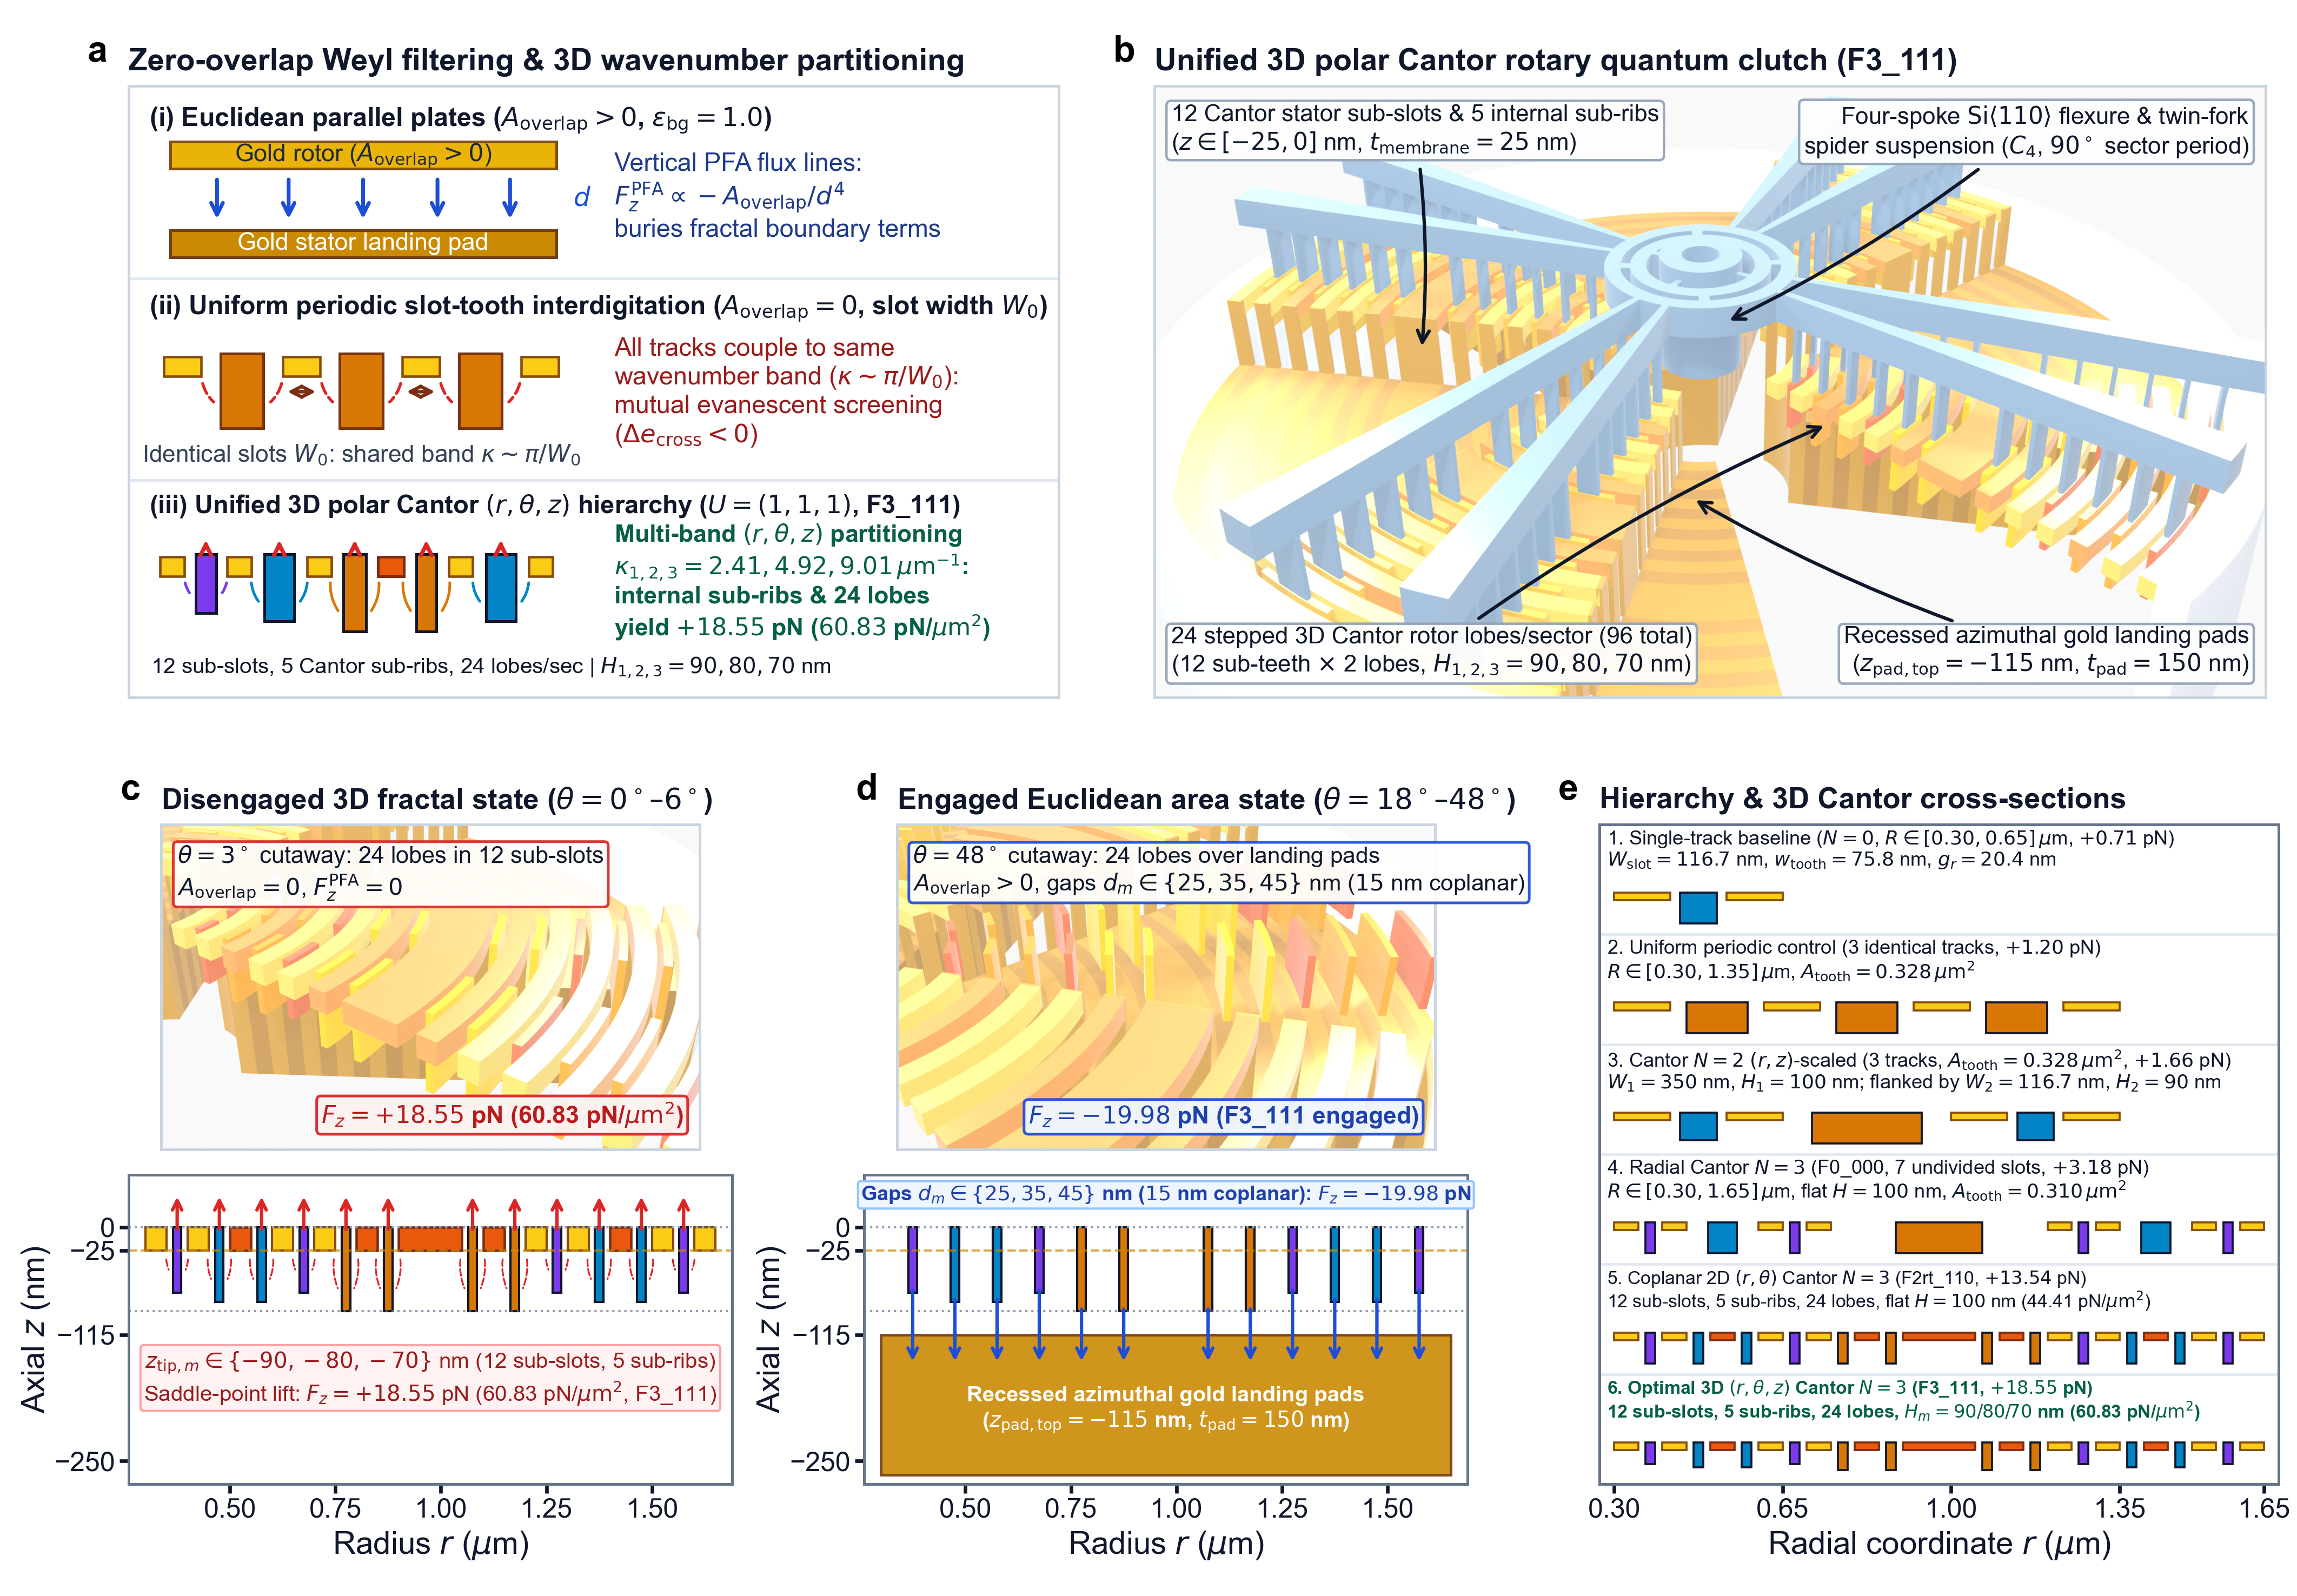
\includegraphics[width=0.95\textwidth]{figures/fig_rotational_z_eff_clutch_blender.png}
\caption{\textbf{Zero-overlap PFA cancellation and 3D rotational clutch architecture in vacuum ($\varepsilon_{\rm bg}=1.0$).} \textbf{a}, Two-dimensional cross-sectional schematic comparing Euclidean parallel plates ($A_{\rm overlap} > 0$, dominated by attractive proximity-force scaling $F_z^{\rm PFA} \propto -A_{\rm overlap}/d^4$), uniform periodic slot-tooth interdigitation ($A_{\rm overlap} = 0$, limited by single-scale evanescent screening at $\kappa \sim \pi/W_0$), and prefractal Cantor interdigitation ($W_k = W_1 b^{-(k-1)}$, stepped depths $H_k$, partitioning transverse fringing fields across separated wavenumber bands). \textbf{b}, Three-dimensional cutaway render of the four-fold symmetric ($C_4$, $90^\circ$ sector period) concentric gold rotor and stator in the disengaged open-slot state ($\theta = 3^\circ$). Downward-protruding concentric rotor teeth ($z \in [-100, 0]\text{ nm}$, $H_1 = \CantorNtwoHybridrzHGenoneNm{}\text{ nm}$, $H_2 = \CantorNtwoHybridrzHGentwoNm{}\text{ nm}$) interdigitate radially inside thin slotted Cantor stator aperture rings ($25\text{ nm}$ membrane thickness, $z \in [-25, 0]\text{ nm}$) suspended above recessed azimuthal landing pads ($150\text{ nm}$ thickness, top surface at $z = -115\text{ nm}$) and supported by a four-spoke $\text{Si}\langle 110\rangle$ flexure suspension. \textbf{c},\textbf{d}, Cutaway renders and axial-radial $(r,z)$ cross-sections in (\textbf{c}) the disengaged open-slot state ($\theta = 0^\circ\text{--}6^\circ$, $A_{\rm overlap} = 0$, $F_z^{\rm PFA} = 0$, showing upward saddle-point repulsive force $F_z = +\roundtwo{\FractalNthreeCantorseventrackBemThetathreeFZPn}\text{ pN}$ at $z_{\rm tip} = -100\text{ nm}$ for $N=3$ on the \texttt{Standard} BEM mesh) and (\textbf{d}) the engaged landing-pad state ($\theta = 18^\circ\text{--}48^\circ$, $A_{\rm overlap} > 0$ across the $d = 15\text{ nm}$ vertical gap, showing normal attraction $F_z = \roundtwo{\FractalNthreeCantorseventrackBemThetafoureightFZPn}\text{ pN}$ for $N=3$). \textbf{e}, Radial cross-sectional profiles comparing the single-track baseline ($N=0$), first-generation slot ($N=1$), uniform periodic and monotonic controls, stepped $(r,z)$ $N=2$ Cantor ring, and seven-track $N=3$ Cantor ring across $r \in [0.30, 1.65]\ \mu\text{m}$.}
\label{fig:rotational_clutch_architecture}
\end{figure*}

% Subheading 2: <= 40 characters including spaces (38 chars)
\section*{Multiscale Cantor force amplification}
\label{sec:repulsion_physics}

\begin{figure*}[t]
\centering
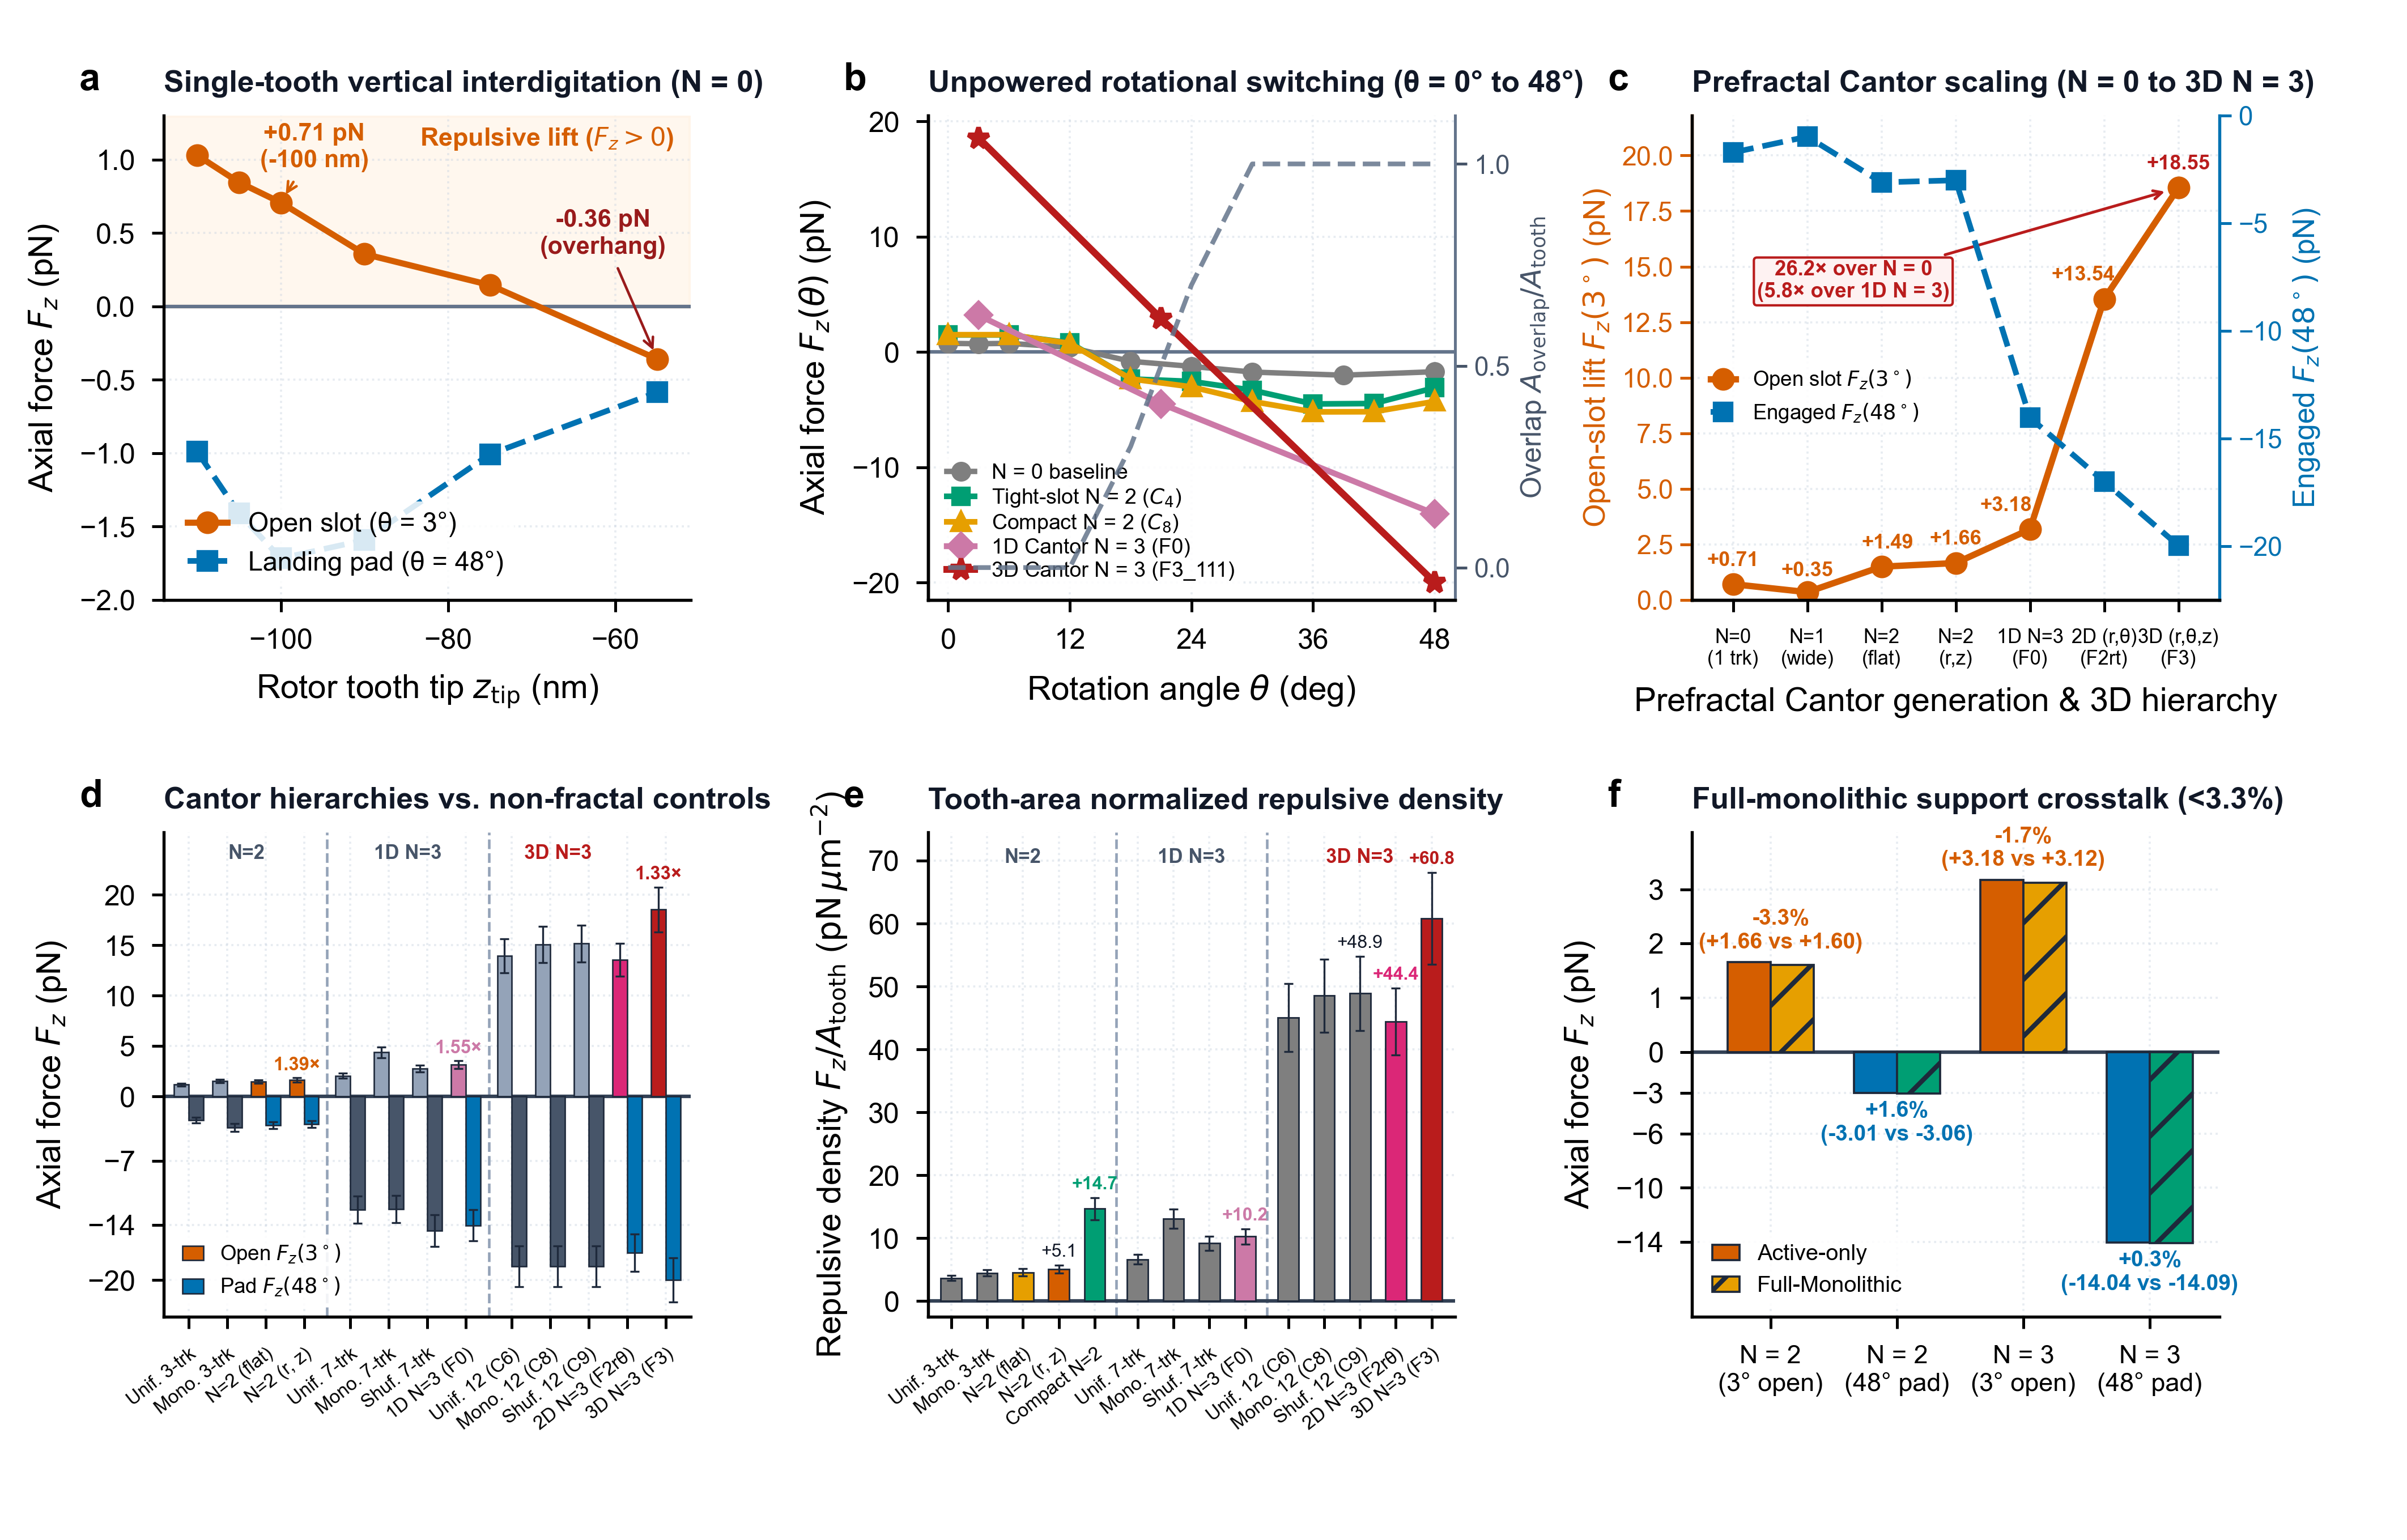
\includegraphics[width=0.95\textwidth]{figures/fig_nature_6step_narrative.png}
\caption{\textbf{Multiscale Cantor force amplification and rotational switching across the six-step benchmark in vacuum ($\varepsilon_{\rm bg}=1.0$).} \textbf{a}, Single-tooth vertical interdigitation ($N=0$) across tooth tip elevation $z_{\rm tip} \in [-115, -55]\text{ nm}$, showing open-slot repulsive force ($+\roundtwo{\SingletoothTrackzeroBemThetathreeFZPn}\text{ pN}$ at $z_{\rm tip} = -100\text{ nm}$) and sign reversal to attraction ($\roundtwo{\SingletoothTrackzeroOverhangBemThetathreeFZPn}\text{ pN}$) under symmetric overhang ($z_{\rm tip} = -55\text{ nm}$). \textbf{b}, Zero-bias rotational switching ($\theta = 0^\circ$ to $48^\circ$) of axial Casimir force $F_z(\theta)$ (left axis) and normalized landing-pad overlap fraction $A_{\rm overlap}/A_{\rm tooth}$ (right axis) across the $N=0$ baseline, tight-slot $N=2$, compact $N=2$, and seven-track $N=3$ Cantor clutches. \textbf{c}, Progression across prefractal generations $N = 0 \to 3$ on the matched \texttt{Standard} BEM mesh, reaching $+\roundtwo{\FractalNthreeCantorseventrackBemThetathreeFZPn}\text{ pN}$ open-slot repulsive force ($\FractalNthreeVsNzeroBemStdRatio{}\times$ over $N=0$) and $\roundtwo{\FractalNthreeCantorseventrackBemThetafoureightFZPn}\text{ pN}$ engaged attraction at $N=3$. \textbf{d}, Comparison of $N=2$ (3-track) and $N=3$ (7-track) Cantor hierarchies against matched non-fractal control families (single wide tooth, 3-track and 7-track uniform periodic gratings, size-matched monotonic arrays, and randomly permuted 7-track control). \textbf{e}, Active-tooth-area normalized repulsive force density $F_z/A_{\rm tooth}$ across all evaluated $N=2$ and $N=3$ hierarchies and controls. \textbf{f}, Active-only versus full-monolithic NEMS structural assemblies incorporating spider spokes, hub collars, and substrate trenches ($<3.3\%$ support crosstalk).}
\label{fig:quantum_clutch_architecture_and_narrative}
\end{figure*}

\begin{figure*}[t]
\centering
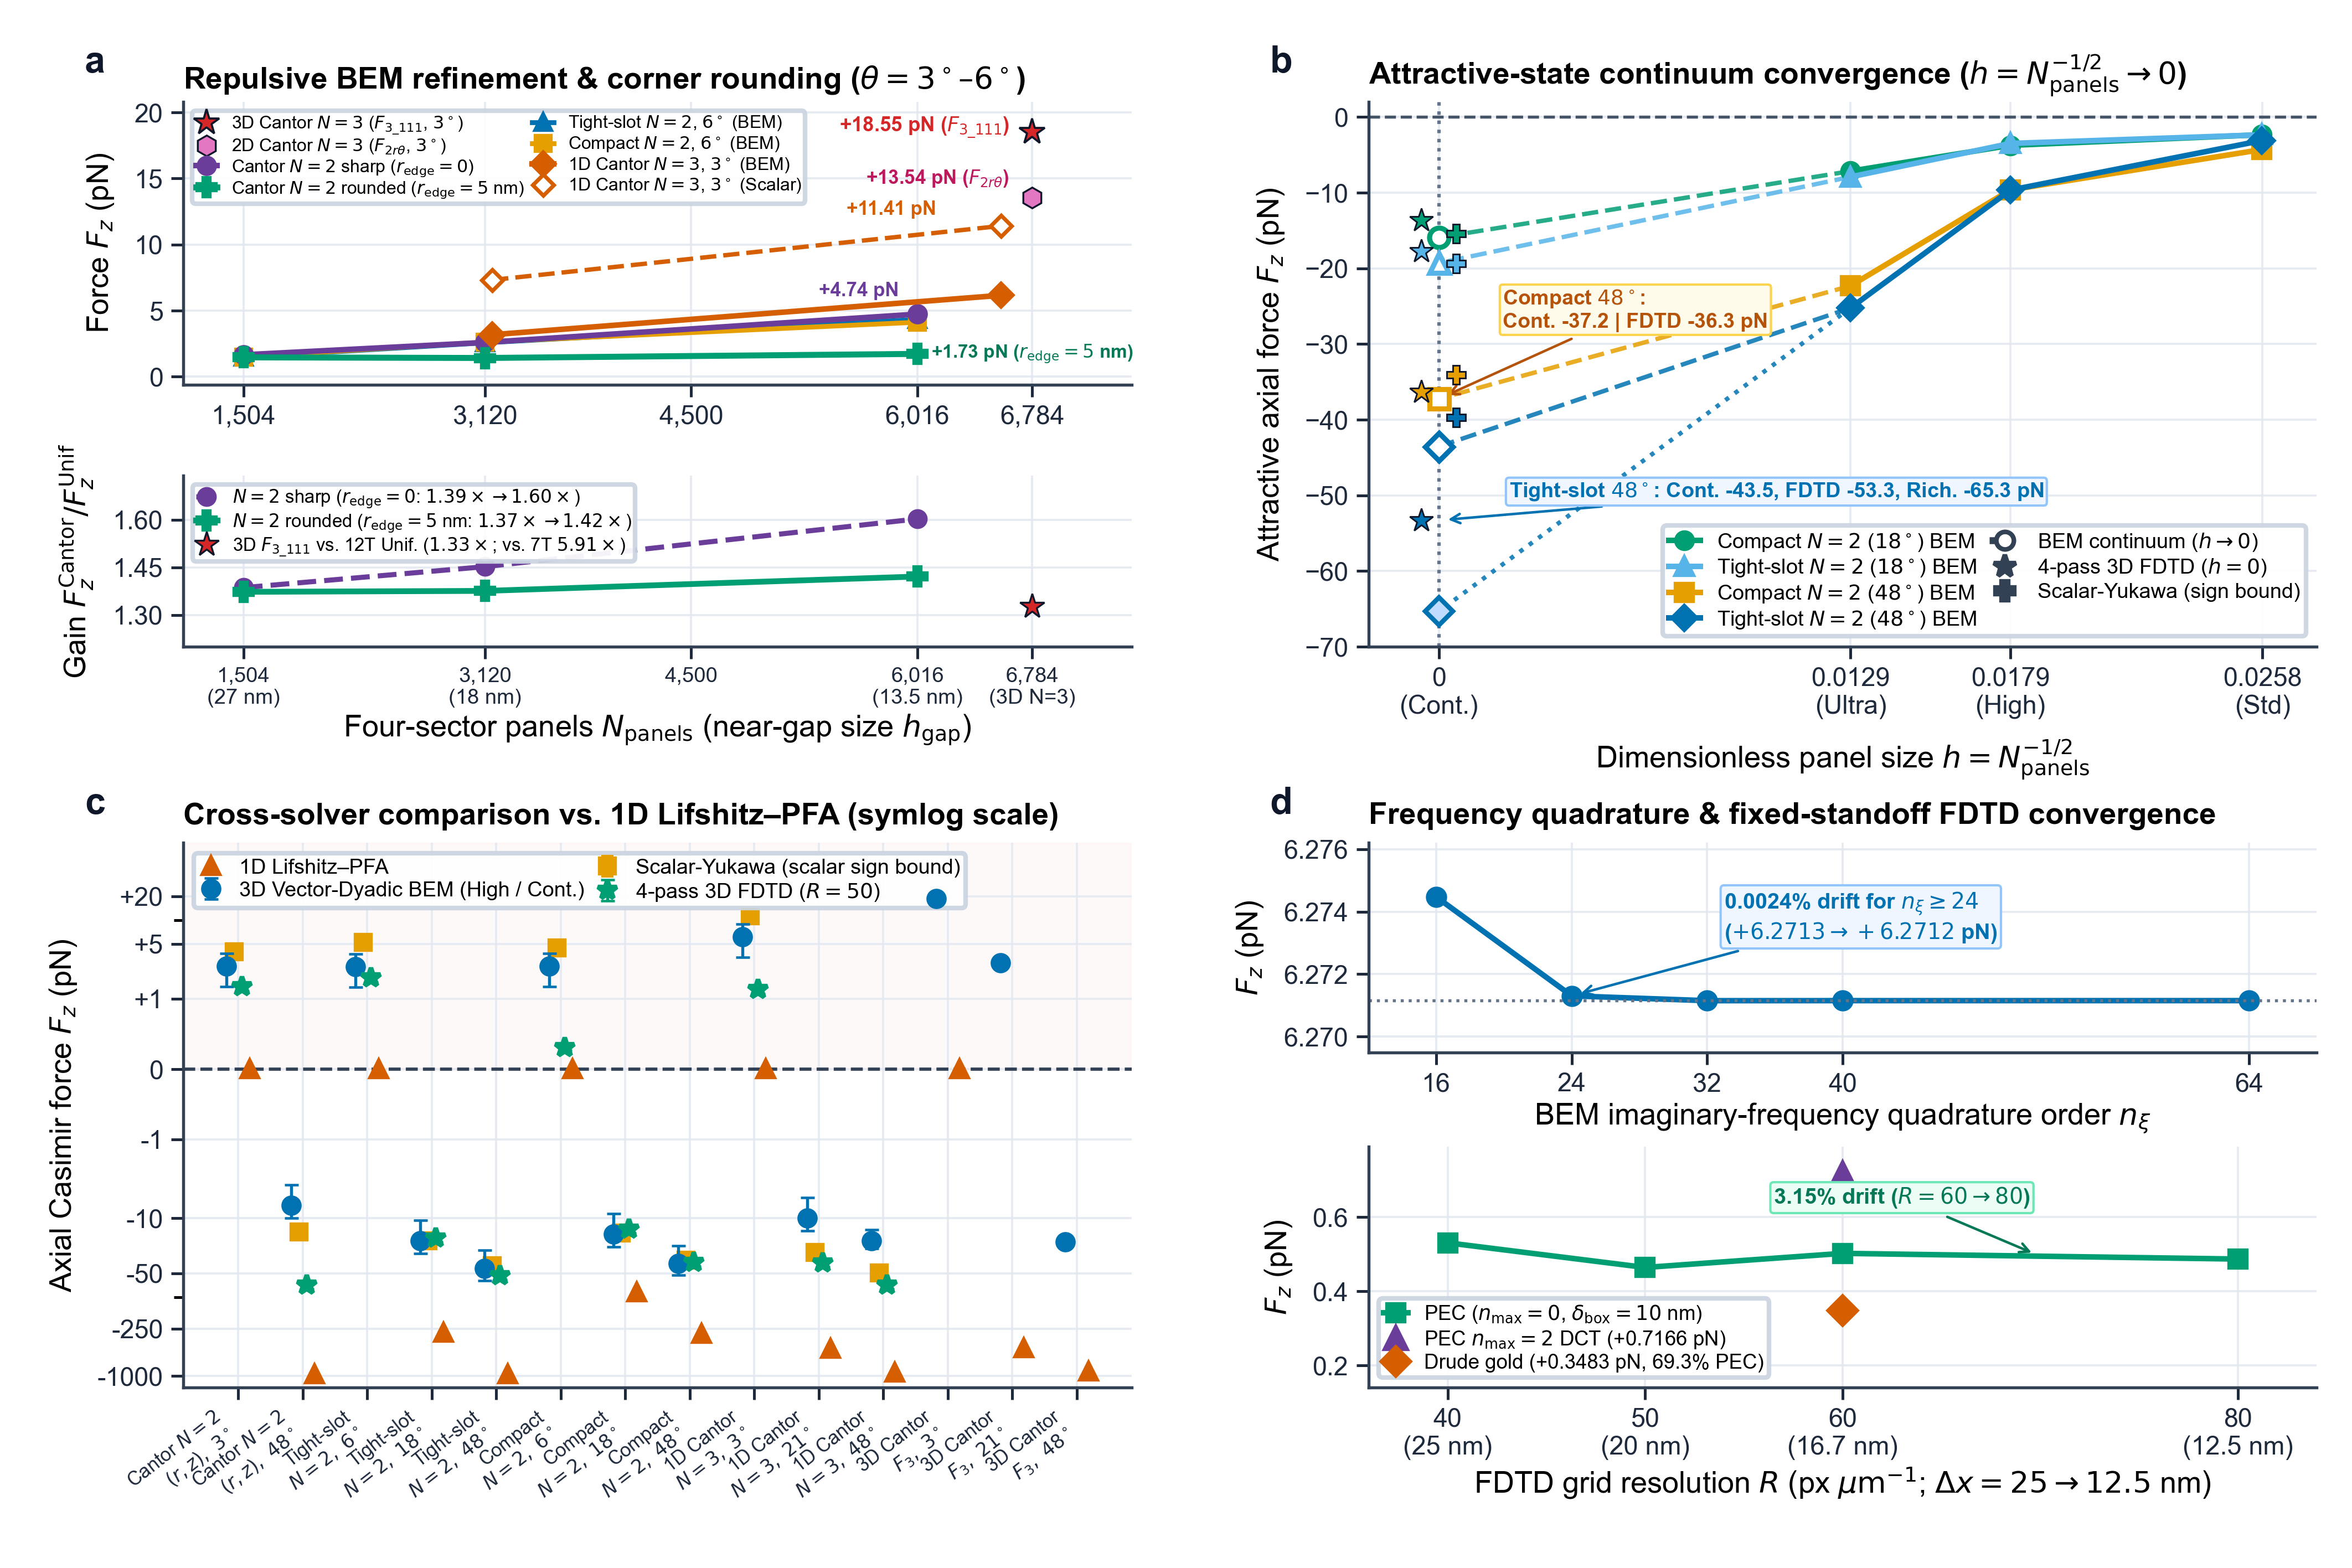
\includegraphics[width=0.95\textwidth]{figures/fig_rotational_clutch_3solver_verification.png}
\caption{\textbf{Discretization sensitivity, corner-rounding regularization, and cross-solver benchmarks in vacuum ($\varepsilon_{\rm bg}=1.0$).} \textbf{a}, Repulsive-state ($\theta = 3^\circ\text{--}6^\circ$) surface-mesh refinement across \texttt{Standard} ($\RotCfourTightslotNtwoStandardThetaZerozerosixpzeroPanelCount{}$ panels), \texttt{High} ($\RotCfourTightslotNtwoHighThetaZerozerosixpzeroPanelCount{}$ panels), and \texttt{Ultra-High} ($\RotCfourTightslotNtwoUltraHighThetaZerozerosixpzeroPanelCount{}$ panels) discretizations for $N=2$ ($\RotConezeroFractalNthreeStandardThetaZerozerothreepzeroPanelCount{}$ and $\RotConezeroFractalNthreeHighThetaZerozerothreepzeroPanelCount{}$ panels for $N=3$) comparing sharp-edge ($r_{\rm edge} = 0$) and lithographically rounded ($r_{\rm edge} = 5\text{ nm}$) 3D Vector-Dyadic BEM and diagnostic 3D Scalar-Yukawa BEM (top), alongside the Cantor-to-uniform repulsive gain ratio $F_z^{\rm Cantor}/F_z^{\rm unif}$ across mesh tiers (bottom). \textbf{b}, Attractive-state ($\theta = 18^\circ\text{--}48^\circ$) boundary-element continuum extrapolations ($h = N_{\rm panels}^{-1/2} \to 0$) compared against 4-pass inclusion--exclusion 3D FDTD MEEP benchmarks and Scalar-Yukawa High-mesh bounds. \textbf{c}, Cross-solver sign and magnitude comparison (on a symmetric logarithmic scale) across 3D Vector-Dyadic BEM, 3D Scalar-Yukawa BEM, 4-pass 3D FDTD ($R=50$), and 1D Lifshitz--PFA across disengaged repulsive, transition, and engaged attractive rotor angles. \textbf{d}, Imaginary-frequency Gauss--Legendre quadrature convergence across $n_\xi \in \{16, 24, 32, 40, 64\}$ ($\roundfour{\BemConvNxiDriftPct}\%$ drift for $n_\xi \ge 24$, top) and fixed-standoff ($\delta_{\rm box} = \MeepFixedboxMarginNm{}\text{ nm}$) 4-pass FDTD resolution scaling across $R \in \{40, 50, 60, 80\}$ ($\roundtwo{\MeepFixedboxRsixzeroToReightzeroDriftPct}\%$ drift between $R=60$ and $R=80$, bottom).}
\label{fig:quantum_clutch_3solver_verification}
\end{figure*}

We evaluate the 3D electromagnetic Casimir forces in vacuum using a custom $C_4$-symmetric 3D Vector-Dyadic boundary-element method (BEM) with dispersive Drude gold across matched surface discretizations, and compare the force sign, angular switching, and discretization sensitivity against 4-pass 3D finite-difference time-domain (FDTD) simulations and a diagnostic 3D Scalar-Yukawa BEM model\cite{rodriguez2009pra,oskooi2010,rodriguez2011,reid2013pra} (Figs.~\ref{fig:quantum_clutch_architecture_and_narrative} and \ref{fig:quantum_clutch_3solver_verification}, Extended Data Tables~\ref{tab:fractal_geometry_control} and \ref{tab:quantum_clutch}, and Methods). Because unrounded $90^\circ$ metallic corners exhibit singular edge-current crowding ($\rho \sim r_{\rm edge}^{-1/3}$) that causes raw BEM forces on sharp edges to grow with panel density, all comparative geometry benchmarks in Fig.~\ref{fig:quantum_clutch_architecture_and_narrative} and Extended Data Table~\ref{tab:fractal_geometry_control} are evaluated at matched \texttt{Standard} panel density; we then show in Fig.~\ref{fig:quantum_clutch_3solver_verification}a and Extended Data Table~\ref{tab:quantum_clutch} that introducing a physical $r_{\rm edge} = 5\text{ nm}$ lithographic corner radius regularizes the mesh-refinement slope ($+1.463 \to +1.416 \to +1.725\text{ pN}$ on the hybrid $N=2$ Cantor ring versus $+1.066 \to +1.029 \to +1.215\text{ pN}$ on the uniform three-track grating) while preserving a stable Cantor-over-uniform amplification ratio of $1.37\times\text{--}1.42\times$ across all mesh tiers.

On the single-track baseline ($N=0$), deep interdigitation of the rotor tooth inside the open stator slot at $\theta=3^\circ$ ($z_{\rm tip} = -100\text{ nm}$, extending $75\text{ nm}$ below the stator ring bottom) generates an upward repulsive axial force of $+\roundtwo{\SingletoothTrackzeroBemThetathreeFZPn}\text{ pN}$, which switches to parallel-plate attraction of $\roundtwo{\SingletoothTrackzeroBemThetafoureightFZPn}\text{ pN}$ when rotated over the landing pad at $\theta=48^\circ$ (Fig.~\ref{fig:quantum_clutch_architecture_and_narrative}a,b). Retracting the tooth upward to $z_{\rm tip} = -55\text{ nm}$ so that its top face overhangs the stator upper plane by $+45\text{ nm}$ reverses the vertical asymmetry across the slot mid-plane and flips the $\theta=3^\circ$ open-slot force from repulsion to attraction ($\roundtwo{\SingletoothTrackzeroOverhangBemThetathreeFZPn}\text{ pN}$), confirming that axial repulsion originates from saddle-point sidewall fringing\cite{levin2010}.

Single-scale interdigitation, however, fails to scale across a wide annular cavity (Fig.~\ref{fig:quantum_clutch_architecture_and_narrative}c--e and Extended Data Table~\ref{tab:fractal_geometry_control}). Widening a single tooth across the radial span moves the stator slot sidewalls far from the tooth centre, collapsing the transverse fringing gradient and eliminating open-slot repulsion ($F_z = \roundtwo{\CtrlSinglewideBemThetathreeFZPn}\text{ pN}$ at $\theta=3^\circ$). Similarly, the single wide first-generation Cantor slot ($N=1$) yields only $+\roundtwo{\FractalNoneFundringBemThetathreeFZPn}\text{ pN}$ at $\theta=3^\circ$. When the $R \in [0.30, 1.35]\ \mu\text{m}$ annulus is subdivided into a three-track uniform periodic grating of equal active tooth area ($A_{\rm tooth} = \roundthree{\FractalCtrlUniformperiodicActiveToothAreaUmtwo}\ \mu\text{m}^2$, edge perimeter $P_{\rm edge} = \roundtwo{\FractalCtrlUniformperiodicEdgePerimeterUm}\ \mu\text{m}$), all slots share a single width and couple to the same evanescent wavenumber band; mutual screening between adjacent tracks limits $\theta=3^\circ$ repulsion to $+\roundtwo{\CtrlUniformperiodicBemThetathreeFZPn}\text{ pN}$ ($\roundtwo{\NatureCtrlUniformperiodicFRepPnPerToothAreaUmtwo}\text{ pN}\,\mu\text{m}^{-2}$, or $\roundthree{\FractalCtrlUniformperiodicFRepPnPerUm}\text{ pN}\,\mu\text{m}^{-1}$ per unit edge perimeter). By contrast, flanking the central primary slot with two narrower second-generation child tracks at matched tooth area and edge perimeter ($A_{\rm tooth} = \roundthree{\FractalCantorFlatzActiveToothAreaUmtwo}\ \mu\text{m}^2$, $P_{\rm edge} = \roundtwo{\FractalCantorFlatzEdgePerimeterUm}\ \mu\text{m}$) in the uniform-depth $N=2$ Cantor ring elevates $\theta=3^\circ$ repulsive force to $+\roundtwo{\CantorNtwoFlatzBemThetathreeFZPn}\text{ pN}$ ($\roundtwo{\NatureCantorNtwoFlatzFRepPnPerToothAreaUmtwo}\text{ pN}\,\mu\text{m}^{-2}$, $\roundthree{\FractalCantorFlatzFRepPnPerUm}\text{ pN}\,\mu\text{m}^{-1}$)---a $\CantorNtwoFlatzVsUniformBemStdRatio{}\times$ enhancement over the uniform periodic grating at identical area and perimeter.

Comparing the $N=2$ and $N=3$ Cantor hierarchies against the non-fractal control families disentangles multiscale width polydispersity from spatial track ordering and cylindrical radius (Fig.~\ref{fig:quantum_clutch_architecture_and_narrative}d,e and Extended Data Table~\ref{tab:fractal_geometry_control}). In the three-track ($N=2$) family, ordering the three Cantor track widths monotonically from inner to outer radius shifts the widest $350\text{ nm}$ slot to the outer radius, increasing active tooth area by $+5.7\%$ ($A_{\rm tooth} = \roundthree{\FractalCtrlSizematchedMonotonicActiveToothAreaUmtwo}\ \mu\text{m}^2$) via cylindrical arc length ($R\Delta\theta$) and yielding $+\roundtwo{\CtrlSizematchedMonotonicBemThetathreeFZPn}\text{ pN}$ at $\theta=3^\circ$. Normalized by active tooth area, however, the uniform-depth $N=2$ Cantor ring ($\roundtwo{\NatureCantorNtwoFlatzFRepPnPerToothAreaUmtwo}\text{ pN}\,\mu\text{m}^{-2}$) exceeds the monotonic control ($\roundtwo{\NatureCtrlSizematchedMonotonicFRepPnPerToothAreaUmtwo}\text{ pN}\,\mu\text{m}^{-2}$). Scaling the vertical tooth depths strictly as $H_k = H_1 b^{-(k-1)}$ ($H_1 = 100\text{ nm}, H_2 = 33.3\text{ nm}$ in \texttt{Cantor\_N2\_TrueRZ}) yields $+1.55\text{ pN}$ ($4.73\text{ pN}\,\mu\text{m}^{-2}$, $1.30\times$ over the uniform grating), while empirically optimizing the child-track depth to $H_2 = \CantorNtwoHybridrzHGentwoNm{}\text{ nm}$ in the stepped $(r,z)$ hybrid ring (\texttt{Cantor\_N2\_HybridRZ}, $A_{\rm tooth} = \roundthree{\FractalCantorRzScalematchedActiveToothAreaUmtwo}\ \mu\text{m}^2$) retains deeper sidewall overlap and elevates $\theta=3^\circ$ repulsion to $+\roundtwo{\CantorNtwoHybridrzBemStdFZPn}\text{ pN}$ ($\roundtwo{\NatureCantorNtwoHybridrzFRepPnPerToothAreaUmtwo}\text{ pN}\,\mu\text{m}^{-2}$), surpassing both the three-track monotonic control ($+13.2\%$ in areal density) and the uniform periodic grating ($\CantorNtwoHybridrzVsUniformBemStdRatio{}\times$). Compressing this three-track hierarchy into $R \in [0.20, 0.90]\ \mu\text{m}$ (\texttt{Rot\_C8\_Compact\_N2}, $A_{\rm tooth} = \roundthree{\RotCeightCompactNtwoStandardThetaZerofoureightpzeroPolarOverlapUmtwo}\ \mu\text{m}^2$) achieves $+\roundtwo{\NatureRotCeightCompactNtwoFRepPn}\text{ pN}$ and the highest areal density ($\roundtwo{\NatureRotCeightCompactNtwoFRepPnPerToothAreaUmtwo}\text{ pN}\,\mu\text{m}^{-2}$).

In the wider seven-track ($N=3$) family spanning $R \in [\FractalNthreeCantorseventrackRInUm{}, \FractalNthreeCantorseventrackROutUm{}]\ \mu\text{m}$ ($28$ teeth, $g_{r,3} = \FractalNthreeCantorseventrackGRGenthreeNm{}\text{ nm}$), the seven-track Cantor ring reaches $+\roundtwo{\FractalNthreeCantorseventrackBemThetathreeFZPn}\text{ pN}$ ($\roundtwo{\NatureFractalNthreeCantorseventrackFRepPnPerToothAreaUmtwo}\text{ pN}\,\mu\text{m}^{-2}$ at $\theta=3^\circ$ and $\roundtwo{\FractalNthreeCantorseventrackBemThetafoureightFZPn}\text{ pN}$ at $\theta=48^\circ$). Relative to matched seven-track controls across the identical annulus, the Cantor hierarchy exceeds the equal-width seven-track uniform periodic grating ($+\roundtwo{\NthreeCurvCylUniformFzPn}\text{ pN}$, $6.62\text{ pN}\,\mu\text{m}^{-2}$) by $1.55\times$ and a randomly permuted seven-track ordering ($+\roundtwo{\NthreeCurvCylShuffledFzPn}\text{ pN}$, $9.16\text{ pN}\,\mu\text{m}^{-2}$) by $1.15\times$ (and exceeds the three-track uniform grating by $\FractalNthreeVsUniformBemStdRatio{}\times$ and the smaller-footprint $N=0$ baseline by $\FractalNthreeVsNzeroBemStdRatio{}\times$; Fig.~\ref{fig:quantum_clutch_architecture_and_narrative}c--e). Notably, in this wide $5.5:1$ cylindrical annulus ($R_{\max}/R_{\min} = 1.65/0.30$), ordering the seven multiscale Cantor track widths monotonically from inner to outer radius (\texttt{Ctrl\_Monotonic7Track}, $A_{\rm tooth} = 0.336\ \mu\text{m}^2$) yields $+\roundtwo{\NthreeCurvCylMonotonicFzPn}\text{ pN}$ ($13.07\text{ pN}\,\mu\text{m}^{-2}$, $+\roundone{\NthreeCurvCylMonoVsCantorPct}\%$ above Cantor; Fig.~\ref{fig:quantum_clutch_architecture_and_narrative}d,e and Extended Data Table~\ref{tab:fractal_geometry_control}). A per-track 3D BEM force decomposition ($F_z = \sum_{k=1}^7 F_{z,k}$) and a curvature-decoupling benchmark across a quasi-planar annulus $R \in [10.0, 11.35]\ \mu\text{m}$ ($R_{\max}/R_{\min} = 1.135 \approx 1$ at matched azimuthal arc length) reveal that this $+\roundone{\NthreeCurvCylMonoVsCantorPct}\%$ difference is a cylindrical-curvature effect rather than an intrinsic advantage of monotonic ordering (Methods). Specifically, over $85\%$ of the open-slot repulsion originates from the four narrowest $50\text{ nm}$ slots ($g_{r,3}=15\text{ nm}$), whereas the widest $450\text{ nm}$ slot ($g_{r,1}=135\text{ nm}$) contributes nearly zero axial force ($-0.010$ to $+0.009\text{ pN}$); in the $5.5:1$ cylindrical annulus at fixed angular tooth width $\Delta\theta_{\rm tooth}=12^\circ$, increasing azimuthal chord length $R_k\Delta\theta$ reduces a $50\text{ nm}$ track's repulsive force $2.71$-fold from the innermost radius ($+\roundtwo{\NthreeCurvCylFivezeronmInnerFzPn}\text{ pN}$ at $R_0 = 0.375\ \mu\text{m}$) to the outermost radius ($+\roundtwo{\NthreeCurvCylFivezeronmOuterFzPn}\text{ pN}$ at $R_6 = 1.575\ \mu\text{m}$). Packing all four $50\text{ nm}$ slots at the innermost radii ($\bar{R}_{50} = 0.525\ \mu\text{m}$ in \texttt{Ctrl\_Monotonic7Track}) therefore harvests $+3.86\text{ pN}$ from the $50\text{ nm}$ tracks alone, compared with $+2.72\text{ pN}$ for the radially symmetric Cantor sequence ($\bar{R}_{50} = 0.975\ \mu\text{m}$) and $+\roundtwo{\NthreeCurvCylRevMonotonicFzPn}\text{ pN}$ total for reverse-monotonic outer-packing ($\bar{R}_{50} = 1.425\ \mu\text{m}$). Evaluating $N_{\rm perm} = \roundzero{\NthreePermNEvaluated}$ distinct non-Cantor multiset permutations of $\{50, 50, 50, 50, 150, 150, 450\}\text{ nm}$ in 3D Vector-Dyadic BEM (out of $\frac{7!}{4!\,2!\,1!} = \roundzero{\NthreePermNUniqueMultiset}$ unique multiset permutations) shows that $30/31$ directly evaluated permutations ($96.8\%$, spanning $[+\roundtwo{\NthreePermFzMinPn}, +\roundtwo{\NthreePermFzMaxPn}]\text{ pN}$, mean $+\roundtwo{\NthreePermFzMeanPn}\text{ pN}$, median $+\roundtwo{\NthreePermFzMedianPn}\text{ pN}$) surpass the equal-width uniform control, while the symmetric Cantor sequence sits at the $\roundzero{\NthreePermCantorPctFzEval}\text{th}$ percentile in raw cylindrical force and at the exact median ($\roundzero{\NthreePermCantorPctFcircEval}\text{th}$ percentile, $\sum_k F_{z,k}/(2\pi R_k) = +\roundthree{\NthreeCurvCylCantorFcircPnPerUm}\text{ pN}\,\mu\text{m}^{-1}$) in circumference-normalized force per unit track length. When cylindrical curvature is removed in the large-radius quasi-planar annulus $R \in [10.0, 11.35]\ \mu\text{m}$, the monotonic-over-Cantor gap collapses $\roundone{\NthreeCurvGapReductionFactor}$-fold to just $+\roundtwo{\NthreeCurvQparcMonoVsCantorPct}\%$ ($+\roundtwo{\NthreeCurvQparcMonotonicFzPn}\text{ pN}$ versus $+\roundtwo{\NthreeCurvQparcCantorFzPn}\text{ pN}$, with $+\roundtwo{\NthreeCurvQparcShuffledFzPn}\text{ pN}$ for the shuffled permutation and $+\roundtwo{\NthreeCurvQparcUniformFzPn}\text{ pN}$ for the uniform control), confirming that multiscale slot-width polydispersity ($1.50\times\text{--}1.57\times$ over uniform) is the primary physical mechanism overcoming periodic screening while radial track ordering couples only weakly ($<3\%$) in the absence of cylindrical curvature.

Full-monolithic 3D BEM assemblies incorporating the radial spider spokes, hub collars, and lower substrate trench confirm that passive structural supports perturb the active Casimir force by less than $3.3\%$ on the matched \texttt{Standard} mesh (Fig.~\ref{fig:quantum_clutch_architecture_and_narrative}f and Extended Data Table~\ref{tab:fractal_geometry_control}). Across all three 3D numerical formulations (Fig.~\ref{fig:quantum_clutch_3solver_verification}a--d, Extended Data Table~\ref{tab:quantum_clutch}, and Methods), both BEM kernels and 4-pass 3D FDTD confirm positive repulsive forces in the open-slot regime ($\theta = 0^\circ\text{--}6^\circ$) and sign reversal to strong attraction in the engaged landing-pad regime ($\theta = 18^\circ\text{--}48^\circ$), with continuum-extrapolated Vector-Dyadic BEM intercepts ($-37.23$ to $-65.33\text{ pN}$) bracketing the 4-pass FDTD benchmarks ($-36.30$ to $-53.30\text{ pN}$) at $\theta=48^\circ$, whereas 1D Lifshitz--PFA predicts identically zero force ($\RotCfourTightslotNtwoHighThetaZerozerosixpzeroLifshitzPfaFZPn{}\text{ pN}$) across open slots and overestimates $\theta=48^\circ$ attraction by more than an order of magnitude ($\roundone{\RotCeightCompactNtwoHighThetaZerofoureightpzeroLifshitzPfaFZPn}$ to $\roundone{\RotCfourTightslotNtwoHighThetaZerofoureightpzeroLifshitzPfaFZPn}\text{ pN}$).

% Subheading 3: <= 40 characters including spaces (37 chars)
\section*{Wavenumber and stroke log-periodicity}
\label{sec:log_periodicity_clutch}

\begin{figure*}[t]
\centering
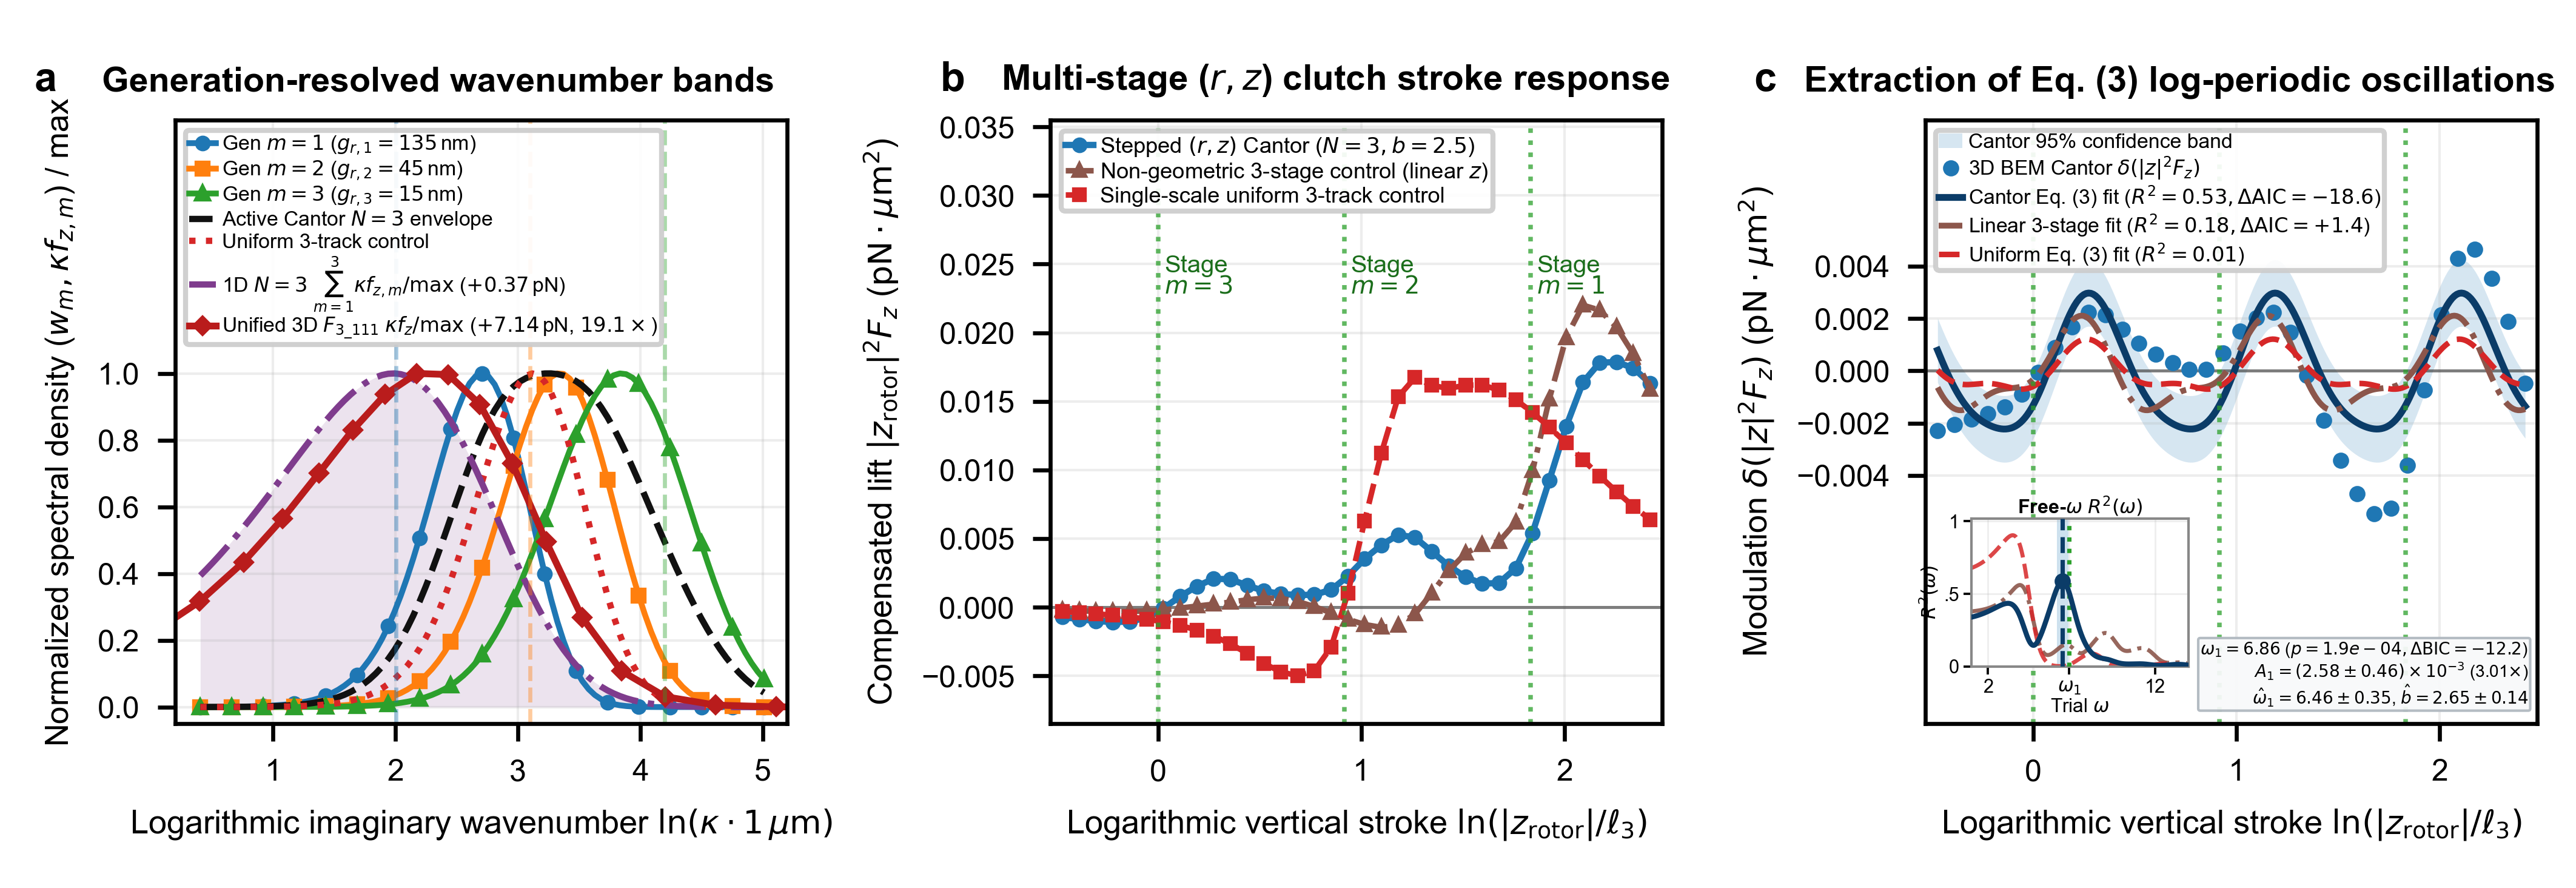
\includegraphics[width=0.98\textwidth]{figures/fig_clutch_log_periodicity.png}
\caption{\textbf{Spectral wavenumber partitioning and multi-stage vertical stroke response in the 3D Cantor clutch in vacuum ($\varepsilon_{\rm bg}=1.0$).} \textbf{a}, Normalized 3D Vector-Dyadic BEM diagnostic radial-wall coupling norm $w_m(\kappa)/\max$ and exact signed Casimir force integrand decomposition $\sum_{m=1}^{3}\kappa f_{z,m}(\kappa)/\max$ (peak $+0.37\text{ pN}$, trace decomposition residual $<10^{-16}\text{ pN}\cdot\mu\text{m}$) across logarithmic imaginary wavenumber $\ln(\kappa \cdot 1\ \mu\text{m})$ for the coplanar third-generation seven-track Cantor ring ($N=3$, $b=3$, radial clearances $g_{r,1}=135\text{ nm}$, $g_{r,2}=45\text{ nm}$, $g_{r,3}=15\text{ nm}$; spectral peaks at $\ln\kappa = \roundtwo{\LogperLnKPeakLone}, \roundtwo{\LogperLnKPeakLtwo}, \text{and } \roundtwo{\LogperLnKPeakLthree}$) compared against the three-track uniform periodic control. Dashed vertical lines mark the inverse radial clearance scales $\kappa = 1/g_{r,m}$. \textbf{b}, Scale-compensated repulsive force $|z_{\rm rotor}|^2 F_z(z_{\rm rotor})$ swept across $36$ logarithmically spaced vertical stroke depths $|z_{\rm rotor}| \in [25, 450]\text{ nm}$ ($\ln(|z_{\rm rotor}|/\ell_3) \in [-0.47, 2.42]$) in a three-generation $(r,z)$-stepped Cantor clutch ($b=\LogperSteppedRzBScale{}$, geometrically spaced stator stage elevations $|z_{{\rm stage},m}| \in \{250, 100, 40\}\text{ nm}$) versus a non-geometric three-stage control with linearly spaced elevations ($|z_{\rm stage}| \in \{250, 145, 40\}\text{ nm}$) and a single-scale three-track uniform control ($|z_{\rm stage}| = 100\text{ nm}$). Dotted vertical lines indicate the designed logarithmic stage intervals $\Delta\ln|z| = \ln b = \roundthree{\LogperSteppedRzLnB}$. \textbf{c}, Detrended modulation $\delta(|z|^2 F_z)$ and $95\%$ regression confidence band from a simultaneous joint quadratic-plus-harmonic least-squares fit to Eq.~\eqref{eq:fourier_running} at the geometric scaling frequency $\omega_1 = 2\pi/\ln b = \roundtwo{\LogperSteppedRzOmegaone}$ ($R^2 = \roundtwo{\LogperSteppedRzRtwo}$, $F = \roundtwo{\LogperSteppedRzFstatCantor}$, $p = 1.9 \times 10^{-4}$, $\Delta\mathrm{AIC} = \roundone{\LogperSteppedRzDeltaAicCantor}$, $\Delta\mathrm{BIC} = \roundone{\LogperSteppedRzDeltaBicCantor}$ for the stepped Cantor clutch, versus $R^2 = \roundtwo{\LogperSteppedRzRtwoLinear}$, $\Delta\mathrm{AIC} = +\roundone{\LogperSteppedRzDeltaAicLinear}$ for the linear three-stage control and $R^2 = \roundtwo{\LogperSteppedRzRtwoUniform}$ for the single-scale uniform control). Inset: unconstrained free-frequency Lomb--Scargle variance-explained spectrum $R^2(\omega)$ swept across $\omega \in [1.0, 14.0]$, recovering $\hat{\omega}_1 = \roundtwo{\LogperFreeOmegaoneCantor} \pm \roundtwo{\LogperFreeOmegaoneCininefiveHalfCantor}$ and scale factor $\hat{b} = \exp(2\pi/\hat{\omega}_1) = \roundtwo{\LogperFreeBHatCantor} \pm \roundtwo{\LogperFreeBHatCininefiveHalfCantor}$ ($95\%\text{ CI}$, peak $R^2(\hat{\omega}_1) = \roundtwo{\LogperFreeRtwoPeakCantor}$).}
\label{fig:clutch_log_periodicity}
\end{figure*}

To examine how the wavenumber partitioning and log-periodic modulation of Eq.~\eqref{eq:fourier_running} manifest in 3D interdigitated rings, we analyze both the imaginary-wavenumber coupling spectrum of a coplanar clutch and the vertical stroke response of a vertically stepped clutch (Fig.~\ref{fig:clutch_log_periodicity} and Methods). In an exact-scaling coplanar $N=3$ Cantor ring ($b=3$, radial clearances $g_{r,m} = g_{r,1} b^{-(m-1)} \in \{135, 45, 15\}\text{ nm}$), all seven concentric tracks engage at a single vertical plane ($z_{\rm tip} = -100\text{ nm}$), superposing all wavenumber contributions at a single stroke depth. Decomposing the diagnostic 3D Vector-Dyadic BEM radial-sidewall coupling norm $w_m(\kappa)$ alongside the exact signed force integrand $\sum_{m=1}^3 \kappa f_{z,m}(\kappa)$ across $\ln\kappa$ illustrates how the three radial clearance generations separate into distinct spectral sub-bands peaking at $\kappa_{{\rm peak},1} = \roundtwo{\LogperKPeakLoneUmInv}\ \mu\text{m}^{-1}$ ($\ln\kappa = \roundtwo{\LogperLnKPeakLone}$), $\kappa_{{\rm peak},2} = \roundtwo{\LogperKPeakLtwoUmInv}\ \mu\text{m}^{-1}$ ($\ln\kappa = \roundtwo{\LogperLnKPeakLtwo}$), and $\kappa_{{\rm peak},3} = \roundtwo{\LogperKPeakLthreeUmInv}\ \mu\text{m}^{-1}$ ($\ln\kappa = \roundtwo{\LogperLnKPeakLthree}$), whereas the three-track uniform periodic control exhibits a single wavenumber band (Fig.~\ref{fig:clutch_log_periodicity}a and Methods). Because finite vertical ring thickness ($H = 100\text{ nm} \sim g_{r,1}$) and gold plasma skin-depth penetration ($\delta_{\rm skin} \approx 22\text{ nm} > g_{r,3}=15\text{ nm}$) regularize the near-field Yukawa decay, the empirical inter-generation peak ratios ($\kappa_{{\rm peak},2}/\kappa_{{\rm peak},1} = \roundtwo{\LogperKPeakRatioTwoone}$ and $\kappa_{{\rm peak},3}/\kappa_{{\rm peak},2} = \roundtwo{\LogperKPeakRatioThreetwo}$) are compressed relative to the idealized knife-edge clearance ratio $b=3$.

This spectral separation highlights a design trade-off between co-focused peak force at a single gap and multi-stage force modulation across a vertical stroke. When all tracks share a common vertical plane ($z_m = z_0$), their repulsive contributions add at one elevation. Conversely, staggering the stator slot centres and track cross-sections geometrically in both radius and vertical elevation as $|z_{{\rm stage},m}| = |z_{{\rm stage},1}| b^{-(m-1)}$ and $\ell_m = \ell_1 b^{-(m-1)}$ ($b=\LogperSteppedRzBScale{}$, $|z_{{\rm stage},m}| \in \{250, 100, 40\}\text{ nm}$; Methods) unfolds the three stages into a sequential, geometrically staged force profile along the vertical rotor coordinate $z_{\rm rotor}$ (Fig.~\ref{fig:clutch_log_periodicity}b,c).

Sweeping the rotor vertically across $36$ logarithmically spaced depths $|z_{\rm rotor}| \in [25, 450]\text{ nm}$ ($\ln(|z_{\rm rotor}|/\ell_3) \in [-0.47, 2.42]$) in 3D Vector-Dyadic BEM shows that as the rotor passes each staggered elevation stage $z_{{\rm stage},m}$, the scale-compensated repulsive force $|z_{\rm rotor}|^2 F_z(z_{\rm rotor})$ exhibits three local maxima spaced by the designed logarithmic stage interval $\Delta\ln|z| \approx \ln b = \roundthree{\LogperSteppedRzLnB}$ (Fig.~\ref{fig:clutch_log_periodicity}b). To quantify how closely this multi-stage stroke response follows the log-periodic functional form of Eq.~\eqref{eq:fourier_running} relative to non-geometric staging, we fit $|z|^2 F_z$ via a joint quadratic-plus-harmonic ordinary least-squares regression at the geometric scaling frequency $\omega_1 = 2\pi/\ln b = \roundtwo{\LogperSteppedRzOmegaone}$ and via an unconstrained free-frequency nonlinear / Lomb--Scargle sweep across $\omega \in [1.0, 14.0]$ (Fig.~\ref{fig:clutch_log_periodicity}c, inset, and Methods). At $\omega_1 = \roundtwo{\LogperSteppedRzOmegaone}$, the geometrically stepped Cantor clutch yields a fundamental harmonic amplitude of $A_1 = (2.58 \pm 0.46) \times 10^{-3}\text{ pN}\cdot\mu\text{m}^2$ ($R^2 = \roundtwo{\LogperSteppedRzRtwo}$, regression $F = \roundtwo{\LogperSteppedRzFstatCantor}$, $p = 1.9 \times 10^{-4}$, $\Delta\mathrm{AIC} = \roundone{\LogperSteppedRzDeltaAicCantor}$, $\Delta\mathrm{BIC} = \roundone{\LogperSteppedRzDeltaBicCantor}$ relative to the quadratic baseline), exceeding the single-stage uniform control ($A_1 = \roundfour{\LogperSteppedRzAmponeUniform}\text{ pN}\cdot\mu\text{m}^2$, $R^2 = \roundtwo{\LogperSteppedRzRtwoUniform}$) by $\roundtwo{\LogperSteppedRzAmponeRatio}\times$ in amplitude, whereas a non-geometric three-stage control with linearly spaced stator elevations ($|z_{\rm stage}| \in \{250, 145, 40\}\text{ nm}$) produces a non-log-periodic profile that is penalized at $\omega_1 = 2\pi/\ln b$ ($R^2 = \roundtwo{\LogperSteppedRzRtwoLinear}$, $\Delta\mathrm{AIC} = +\roundone{\LogperSteppedRzDeltaAicLinear}$; Fig.~\ref{fig:clutch_log_periodicity}b,c). Sweeping the trial scaling frequency freely across $\omega \in [1.0, 14.0]$ without fixing $\omega_1$ in advance recovers a sharp unconstrained spectral peak at $\hat{\omega}_1 = \roundtwo{\LogperFreeOmegaoneCantor} \pm \roundtwo{\LogperFreeOmegaoneCininefiveHalfCantor}$ ($95\%\text{ CI } [\roundtwo{\LogperFreeOmegaoneCininefiveLowCantor}, \roundtwo{\LogperFreeOmegaoneCininefiveHighCantor}]$, peak $R^2(\hat{\omega}_1) = \roundtwo{\LogperFreeRtwoPeakCantor}$), corresponding to an empirical scale factor $\hat{b} = \exp(2\pi/\hat{\omega}_1) = \roundtwo{\LogperFreeBHatCantor} \pm \roundtwo{\LogperFreeBHatCininefiveHalfCantor}$ ($95\%\text{ CI } [\roundtwo{\LogperFreeBHatCininefiveLowCantor}, \roundtwo{\LogperFreeBHatCininefiveHighCantor}]$; two-harmonic refinement $\hat{\omega}_{1,\rm 2h} = \roundtwo{\LogperFreeOmegaoneTwohCantor} \pm \roundtwo{\LogperFreeOmegaoneTwohCininefiveHalfCantor}$, $\hat{b}_{\rm 2h} = \roundtwo{\LogperFreeBHatTwohCantor} \pm \roundtwo{\LogperFreeBHatTwohCininefiveHalfCantor}$), whereas both controls collapse near $\omega_1$ ($R^2_1(\omega_1) = \roundtwo{\LogperFreeRtwoAtOmegaoneLinear}$ and $\roundtwo{\LogperFreeRtwoAtOmegaoneUniform}$, peaking instead at low-frequency turnover modes $\hat{\omega}_{\rm lin} = \roundtwo{\LogperFreeOmegaoneLinear}$ and $\hat{\omega}_{\rm unif} = \roundtwo{\LogperFreeOmegaoneUniform}$; Fig.~\ref{fig:clutch_log_periodicity}c, inset). While geometrically staggering the vertical stages trades single-depth peak force ($+\roundtwo{\LogperSteppedRzMaxFzCantorPn}\text{ pN}$ at $|z_{\rm rotor}| = 53\text{ nm}$ and $+\roundtwo{\LogperSteppedRzStagetwoFzCantorPn}\text{ pN}$ at $118\text{ nm}$, versus $+\roundtwo{\CantorNtwoHybridrzBemStdFZPn}\text{--}\roundtwo{\FractalNthreeCantorseventrackBemThetathreeFZPn}\text{ pN}$ in the coplanar rings), it maintains continuous open-slot repulsion ($F_z > 0$) across an eight-fold vertical stroke range ($|z_{\rm rotor}| \in [45, 360]\text{ nm}$), including sub-$100\text{ nm}$ depths where the single-stage uniform control flips to attraction ($F_z = \roundtwo{\LogperSteppedRzMinFzUniformPn}\text{ pN}$ at $|z_{\rm rotor}| = 73\text{ nm}$).

% Subheading 4: <= 40 characters including spaces (37 chars)
\section*{Room-temperature mechanical stability}
\label{sec:experimental}

\begin{figure*}[t]
\centering
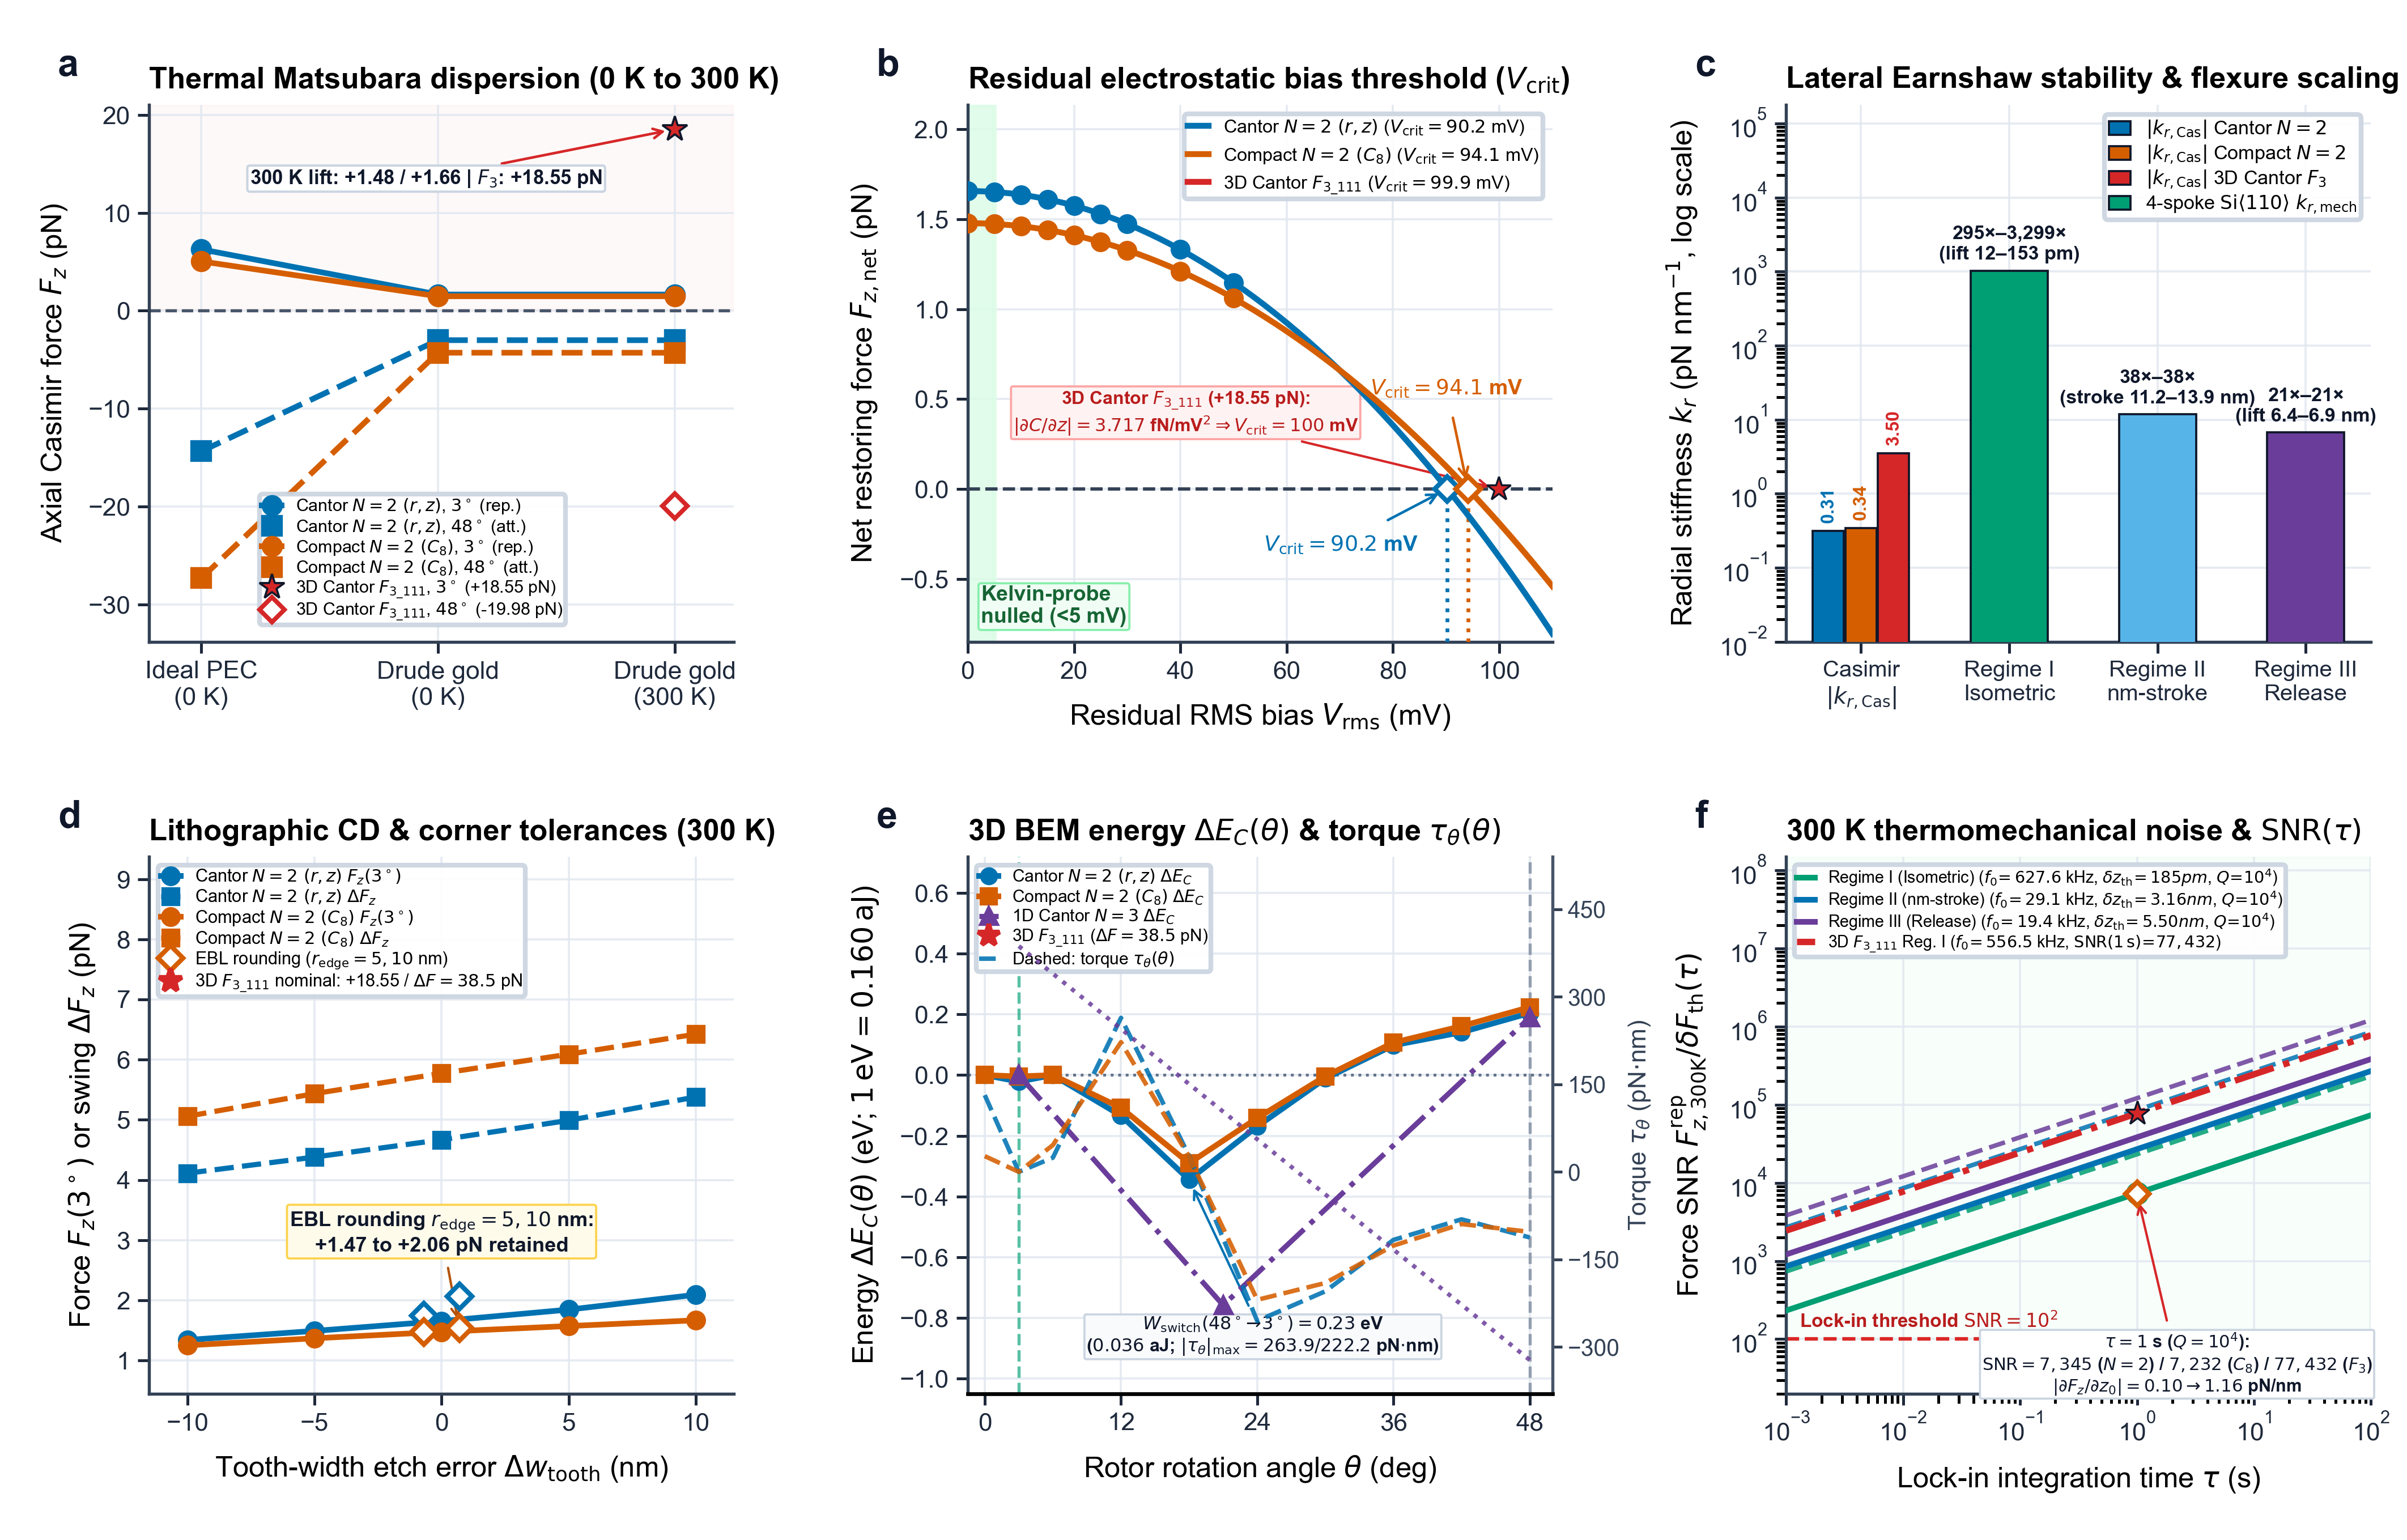
\includegraphics[width=0.95\textwidth]{figures/fig_nature_feasibility_stability.png}
\caption{\textbf{Room-temperature ($T=\NatureRotCeightCompactNtwoCdToleranceTemperatureK{}\text{ K}$) thermal dispersion, electrostatic bias thresholds, flexure scaling, fabrication tolerances, rotational energy/torque, and thermomechanical lock-in SNR in vacuum ($\varepsilon_{\rm bg}=1.0$).} \textbf{a}, Thermal Matsubara dispersion across ideal PEC ($0\text{ K}$), Drude gold ($0\text{ K}$), and room-temperature Drude gold ($300\text{ K}$) for the stepped $(r,z)$ $N=2$ Cantor ring and compact $N=2$ variant on the \texttt{Standard} BEM mesh. \textbf{b}, Net repulsive restoring force $F_{z,\rm net}$ across residual root-mean-square electrostatic bias voltages $V_{\rm rms} \in [0, 100]\text{ mV}$, showing the critical uniform-bias thresholds ($V_{\rm crit} = \roundone{\NatureCantorNtwoHybridrzPatchPotentialVCritMv}\text{ mV}$ and $\roundone{\NatureRotCeightCompactNtwoPatchPotentialVCritMv}\text{ mV}$) and the $<5\text{ mV}$ Kelvin-probe nulled mean-potential regime. \textbf{c}, Destabilizing radial Earnshaw Casimir stiffness $|k_{r,\rm Casimir}|$ compared on a logarithmic scale against the stabilizing four-spoke single-crystal $\text{Si}\langle 110\rangle$ radial flexure stiffness $k_{r,\rm mech}$ ($E_Y = \scinum{\NatureRotCeightCompactNtwoLateralStabilityEYPa}\text{ Pa}$) across isometric transducer (Regime~I), nanometre-stroke (Regime~II), and contact-release clutch (Regime~III) suspensions. \textbf{d}, Room-temperature open-slot repulsive force $F_z(3^\circ)$ and rotational switching swing $\Delta F_z$ across critical-dimension tooth-width etch biases $\Delta w_{\rm tooth} \in [-10, +10]\text{ nm}$ and EBL corner rounding $r_{\rm edge} = 5\text{--}10\text{ nm}$. \textbf{e}, 3D Vector-Dyadic BEM rotational Casimir interaction energy landscape $\Delta E_C(\theta) = E_C(\theta) - E_C(0^\circ)$ (left axis) and axial-switching Casimir torque $\tau_\theta(\theta) = -\partial E_C(\theta)/\partial\theta$ (right axis) across $\theta \in [0^\circ, 48^\circ]$, highlighting the $\theta=18^\circ\text{--}21^\circ$ sidewall-crossing potential well, state-to-state switching work $W_{\rm switch}(48^\circ\!\to\!3^\circ) = 0.23\text{ eV}$, and peak torque $|\tau_\theta|_{\max} = 285\text{--}332\text{ pN}\cdot\text{nm}$. \textbf{f}, Room-temperature ($300\text{ K}$) thermomechanical lock-in force signal-to-noise ratio $\mathrm{SNR}(\tau) = F_{z,300\rm K}^{\rm rep}/\delta F_{\rm th}(\tau)$ versus integration time $\tau \in [10^{-3}, 10^2]\text{ s}$ across Regimes~I--III for ultra-high-vacuum quality factors $Q = 10^4$ (solid) and $Q = 10^5$ (dashed), showing $\mathrm{SNR}(1\text{ s}) = 1{,}155\text{--}1{,}307$ in Regime~I ($f_0 = 2{,}001\text{ kHz}$, $\delta z_{\rm th} = 0.18\text{ nm}$) and $\mathrm{SNR} > 10^2$ across all regimes.}
\label{fig:nature_feasibility_stability}
\end{figure*}

In a nanoelectromechanical system (NEMS) operating at room temperature ($T = \NatureRotCeightCompactNtwoCdToleranceTemperatureK{}\text{ K}$), geometry-induced repulsive Casimir forces must contend with thermal radiation fluctuations, residual electrostatic bias and spatial patch potentials, lateral Earnshaw instability, rotational switching barriers, thermomechanical Brownian motion, and lithographic imperfections. We therefore evaluate finite-temperature Matsubara summation, mutual-capacitance bias thresholds, $\text{Si}\langle 110\rangle$ flexure stiffness scaling, critical-dimension (CD) etch tolerances, 3D rotational energy and torque landscapes, and room-temperature lock-in signal-to-noise ratios across the rotary clutch architectures on the baseline \texttt{Standard} BEM mesh (Fig.~\ref{fig:nature_feasibility_stability}a--f, Extended Data Table~\ref{tab:nems_feasibility}, and Methods).

Matsubara summation at $T = \NatureRotCeightCompactNtwoCdToleranceTemperatureK{}\text{ K}$ shows that room-temperature Drude gold retains a disengaged ($\theta=3^\circ$) repulsive axial force of $+\roundtwo{\NatureCantorNtwoHybridrzPatchPotentialFCasimirGoldThreezerozerokPn}\text{ pN}$ in the stepped $(r,z)$ $N=2$ Cantor ring and $+\roundtwo{\NatureRotCeightCompactNtwoPatchPotentialFCasimirGoldThreezerozerokPn}\text{ pN}$ in the compact $N=2$ variant, while rotating to $\theta=48^\circ$ over the landing pads yields $\roundtwo{\NatureCantorNtwoHybridrzStepfiveForceZPn}\text{ pN}$ and $\roundtwo{\NatureRotCeightCompactNtwoSteptwooneForceZPn}\text{ pN}$ of parallel-plate attraction on the \texttt{Standard} mesh (Fig.~\ref{fig:nature_feasibility_stability}a). While holding the rotor at either $\theta = 3^\circ$ or $\theta = 48^\circ$ requires zero electrical bias, mechanically rotating the rotor between states via an external rotary comb drive traverses a non-monotonic 3D BEM Casimir energy landscape $\Delta E_C(\theta) = E_C(\theta) - E_C(0^\circ)$ featuring an attractive potential well at $\theta = 18^\circ\text{--}21^\circ$ where the rotor tooth edges cross the stator slot sidewalls (Fig.~\ref{fig:nature_feasibility_stability}e). The net state-to-state mechanical switching work is $W_{\rm switch} = |E_C(3^\circ) - E_C(48^\circ)| = 0.23\text{ eV}$ ($0.036\text{ aJ} \approx 8.7\,k_B T_{300}$) for \texttt{Cantor\_N2\_HybridRZ} ($0.26\text{ eV}$ for \texttt{Rot\_C8\_Compact\_N2}), with peak axial-switching Casimir torques $|\tau_\theta|_{\max} = |-\partial E_C/\partial\theta|_{\max} = 285\text{ pN}\cdot\text{nm}$ and $332\text{ pN}\cdot\text{nm}$ at $\theta = 12^\circ$---readily supplied by standard electrostatic rotary comb actuators (Methods). From the 3D BEM mutual-capacitance gradients $|\partial C_{\rm el}/\partial z|$, the critical uniform RMS voltage at which electrostatic attraction $F_{z,\rm el} = -\frac{1}{2}|\partial C_{\rm el}/\partial z|V_{\rm rms}^2$ cancels room-temperature Casimir repulsion is $V_{\rm crit} = \roundone{\NatureCantorNtwoHybridrzPatchPotentialVCritMv}\text{ mV}$ for the stepped $(r,z)$ $N=2$ ring and $\roundone{\NatureRotCeightCompactNtwoPatchPotentialVCritMv}\text{ mV}$ for the compact variant (Fig.~\ref{fig:nature_feasibility_stability}b). This provides an $18\times$ margin above Kelvin-probe-compensated mean contact potential differences ($<5\text{ mV}$), although spatially varying work-function patches on polycrystalline gold (when grain size approaches the $15\text{--}60\text{ nm}$ clearances) cannot be nulled by a single global bias and must be minimized through small-grain deposition or single-crystal/epitaxial gold templates (Methods).

To suppress lateral Earnshaw snap-in across the $15\text{--}60\text{ nm}$ radial slot clearances while allowing axial motion, suspending the stator or rotor frame on a $\NatureRotCeightCompactNtwoLateralStabilitySpokeCount{}$-spoke single-crystal $\text{Si}\langle 110\rangle$ clamped-guided flexure ($E_Y = \scinum{\NatureRotCeightCompactNtwoLateralStabilityEYPa}\text{ Pa}$, decoupled from the coarse rotational drive) exploits the quadratic aspect-ratio ratio $k_{r,\rm mech}/k_{z,\rm mech} = (w_{\rm spoke}/t_{\rm spoke})^2$ between radial and axial translational stiffness (Fig.~\ref{fig:nature_feasibility_stability}c, Extended Data Table~\ref{tab:nems_feasibility}, and Methods). In the stiff isometric regime (Regime~I: $L_{\rm spoke} = \NatureRotCeightCompactNtwoLateralStabilityLSpokeUm{}\ \mu\text{m}$, $k_{z,\rm mech} = \roundone{\NatureRotCeightCompactNtwoLateralStabilityKZMechPnPerNm}\text{ pN}\,\text{nm}^{-1}$, $k_{r,\rm mech} = \roundone{\NatureRotCeightCompactNtwoLateralStabilityKRMechPnPerNm}\text{ pN}\,\text{nm}^{-1}$), the suspension exceeds the destabilizing radial Casimir stiffness ($|k_{r,\rm Casimir}| = \roundthree{\NatureCantorNtwoHybridrzLateralStabilityKRCasimirPnPerNm}\text{ pN}\,\text{nm}^{-1}$ for \texttt{Cantor\_N2\_HybridRZ} and $0.313\text{--}\roundthree{\NatureRotCeightCompactNtwoLateralStabilityOriginEvenEnergyEstimatePnPerNm}\text{ pN}\,\text{nm}^{-1}$ for \texttt{Rot\_C8\_Compact\_N2}) by safety factors of $3{,}010\times\text{--}\roundzero{\NatureCantorNtwoHybridrzLateralStabilityLateralStabilitySafetyFactor}\times$ and prevents vertical pull-in at $\theta=48^\circ$ ($\roundone{\NatureRotCeightCompactNtwoLateralStabilityVerticalPullInSafetyFactor}\times\text{--}\roundone{\NatureCantorNtwoHybridrzLateralStabilityVerticalPullInSafetyFactor}\times$ safety margin against the \texttt{Standard}-mesh engaged force, $\roundtwo{\NatureRotCeightCompactNtwoDiscretizationPullInBoundsSharpUltraSfPullInRegone}\times\text{--}\roundtwo{\NatureCantorNtwoHybridrzDiscretizationPullInBoundsSharpUltraSfPullInRegone}\times$ under the \texttt{Ultra-High} BEM engaged force where $k_{z,\rm crit}^{\rm pull\text{-}in} = \roundtwo{\NatureCantorNtwoHybridrzDiscretizationPullInBoundsSharpUltraKzCritPullInPnPerNm}\text{--}\roundtwo{\NatureRotCeightCompactNtwoDiscretizationPullInBoundsSharpUltraKzCritPullInPnPerNm}\text{ pN}\,\text{nm}^{-1}$, and $\roundtwo{\NatureCantorNtwoHybridrzDiscretizationPullInBoundsContinuumSfPullInRegone}\times$ even against the $\roundtwo{\NatureCantorNtwoHybridrzDiscretizationPullInBoundsContinuumFAttPn}\text{ pN}$ continuum-extrapolated engaged force where $k_{z,\rm crit}^{\rm pull\text{-}in} = \roundtwo{\NatureCantorNtwoHybridrzDiscretizationPullInBoundsContinuumKzCritPullInPnPerNm}\text{ pN}\,\text{nm}^{-1}$, while $r_{\rm edge}=5\text{ nm}$ corner-rounded \texttt{Ultra-High} BEM yields $+\roundtwo{\NatureCantorNtwoHybridrzDiscretizationPullInBoundsRfiveUltraFRepPn}\text{ pN}$ disengaged repulsion and $V_{\rm crit} = \roundone{\NatureCantorNtwoHybridrzDiscretizationPullInBoundsRfiveUltraVCritMv}\text{--}\roundone{\NatureRotCeightCompactNtwoDiscretizationPullInBoundsRfiveUltraVCritMv}\text{ mV}$; Extended Data Table~\ref{tab:nems_feasibility}), operating at a fundamental axial resonance frequency $f_0 = 2{,}001\text{ kHz}$ with static deflection of $\roundtwo{\NatureCantorNtwoHybridrzLateralStabilityEquilibriumAxialRepulsiveLiftPm}\text{--}\roundtwo{\NatureRotCeightCompactNtwoLateralStabilityEquilibriumAxialRepulsiveLiftPm}\text{ pm}$ and RMS thermal displacement $\delta z_{\rm th} = \sqrt{k_B T / k_{z,\rm mech}} = 0.18\text{ nm}$ at $300\text{ K}$. Compliant suspensions (Regime~II: $k_{z,\rm mech} = \roundthree{\NatureRotCeightCompactNtwoLateralStabilityNmActuatorKZMechPnPerNm}\text{ pN}\,\text{nm}^{-1}$, radial safety factor $\roundzero{\NatureCantorNtwoHybridrzLateralStabilityNmActuatorLateralSafetyFactor}\times\text{--}\roundzero{\NatureRotCeightCompactNtwoLateralStabilityNmActuatorLateralSafetyFactor}\times$, $\delta z_{\rm th} = 3.16\text{ nm}$; and Regime~III: $k_{z,\rm mech} = \roundthree{\NatureRotCeightCompactNtwoLateralStabilityCompactClutchKZMechPnPerNm}\text{ pN}\,\text{nm}^{-1}$, radial safety factor $\roundzero{\NatureCantorNtwoHybridrzLateralStabilityCompactClutchLateralSafetyFactor}\times\text{--}\roundzero{\NatureRotCeightCompactNtwoLateralStabilityCompactClutchLateralSafetyFactor}\times$) yield static open-slot repulsive lifts of $\roundtwo{\NatureCantorNtwoHybridrzLateralStabilityNmActuatorBasinEqLiftNm}\text{--}\roundtwo{\NatureCantorNtwoHybridrzLateralStabilityCompactClutchBasinEqLiftNm}\text{ nm}$ and peak-to-peak switching strokes of $\roundtwo{\NatureCantorNtwoHybridrzLateralStabilityNmActuatorPeakToPeakStrokeNm}\text{--}\roundtwo{\NatureRotCeightCompactNtwoLateralStabilityNmActuatorPeakToPeakStrokeNm}\text{ nm}$ when engaging onto a dielectric stop-bumper. Because thermomechanical force noise spectral density scales as $S_F^{1/2} = \sqrt{4 k_B T k_{z,\rm mech}/(\omega_0 Q)} \propto (k_{z,\rm mech} m_{\rm eff})^{1/4}$, lock-in force detection at $T = 300\text{ K}$ ($Q = 10^4\text{--}10^5$) yields an intrinsic thermomechanical $\mathrm{SNR}(\tau=1\text{ s}) = 1{,}155\text{--}1{,}307$ in Regime~I and $>4.7\times 10^3$ in Regimes~II--III, surpassing $\mathrm{SNR} > 10^2$ within millisecond integration times (Fig.~\ref{fig:nature_feasibility_stability}f and Methods). Finally, 3D BEM tolerance sweeps confirm that room-temperature open-slot repulsion and switching swing vary smoothly by less than $18\%$ across $r_{\rm edge} = 5\text{--}10\text{ nm}$ lithographic corner rounding and $\Delta w_{\rm tooth} \in [-10, +10]\text{ nm}$ critical-dimension etch biases (Fig.~\ref{fig:nature_feasibility_stability}d and Extended Data Table~\ref{tab:nems_feasibility}).

In summary, our full-wave calculations demonstrate that combining 3D slot-tooth interdigitation with multiscale Cantor slot hierarchies eliminates parallel-plate PFA attraction in the open-slot state and enhances geometry-induced vacuum Casimir repulsion by $\CantorNtwoFlatzVsUniformBemStdRatio{}\times\text{--}1.55\times$ over matched same-generation uniform periodic gratings ($\FractalNthreeVsUniformBemStdRatio{}\times$ across generations) at matched mesh resolution. By partitioning evanescent fringing fields across separated wavenumber bands and switching to parallel-plate attraction over recessed landing pads at zero electrical bias, multiscale interdigitated rings provide a testable nanomechanical architecture for controlling the sign and magnitude of Casimir forces in vacuum, with prospective extensions to optomechanical and cavity quantum electrodynamic sensing once full Green-tensor scattering is incorporated (Fig.~\ref{fig:nature_feasibility_stability}e,f).

\section*{Methods}
\label{sec:methods}

\subsection*{1D transfer-matrix recursion and motivating log-periodic scaling ansatz}
To motivate the scale-dependent Casimir coefficient $C(d_s, \ln(d/\ell_*))$ in Eqs.~\eqref{eq:trace_running}--\eqref{eq:fourier_running}\cite{gordon2026prd}, we consider the idealized 1D reduced Euclidean Green's function $g(z, z'; \kappa)$ at imaginary wavenumber $\kappa = \sqrt{\zeta^2 + \mathbf{k}_\perp^2}$ across an $N$-th generation pre-Cantor stack $\mathcal{C}_N$ of semitransparent delta-function barriers $V(z) = \lambda_0 \sum_{i \in \mathcal{C}_N} \delta(z - z_i)$ on $[0, d]$:
\begin{equation}
\left[ -\frac{\partial^2}{\partial z^2} + \kappa^2 + V(z) \right] g(z, z'; \kappa) = \delta(z - z').
\end{equation}
In the homogeneous vacuum intervals between barriers, $g(z, z'; \kappa) = A_j e^{-\kappa z} + B_j e^{\kappa z}$, where wave amplitudes across barrier $z_i$ are linked by the single-plate transfer matrix $\mathbf{M}_i(\kappa)$:
\begin{equation}
\mathbf{M}_i(\kappa) = \begin{pmatrix} 1 - \frac{\lambda_0}{2\kappa} & -\frac{\lambda_0}{2\kappa} e^{2\kappa z_i} \\ \frac{\lambda_0}{2\kappa} e^{-2\kappa z_i} & 1 + \frac{\lambda_0}{2\kappa} \end{pmatrix}, \qquad \mathbf{M}_{\rm global}(\kappa) = \prod_{i \in \mathcal{C}_N} \mathbf{M}_i(\kappa).
\end{equation}
For any finite coupling $\lambda_0 < \infty$, high-frequency modes ($\kappa \gg \lambda_0$) tunnel across barriers with transmission probability $|t(\kappa)|^2 = 4\kappa^2 / (4\kappa^{2} + \lambda_0^2) > 0$, establishing global thermal equilibrium across all sub-cavities at temperature $T$ prior to taking the strong-coupling limit\cite{gordon2026prd}. Partitioning the $N$-th generation Cantor stack (scale ratio $b=3$) into its left and right $(N-1)$-th generation sub-stacks yields the functional interaction energy recursion $\Delta e_{\mathcal{C}_N}(d) = 2\Delta e_{\mathcal{C}_{N-1}}(d/b) + \Delta e_{\rm cross}(d; \ell_*)$ in Eq.~\eqref{eq:recursion_main}. In $(3+1)$ dimensions, the interaction energy per unit area carries scaling dimension $[\text{length}]^{-3}$; assuming that in the asymptotic prefractal scaling window $\ell_* \ll d \ll L$ the renormalized cross-talk $\Delta e_{\rm cross}$ approaches a discrete scale-invariant fixed point under spatial dilation $d \to d/b$ ($\Delta e_{\rm hom}(d/b) = b^3 \Delta e_{\rm hom}(d)$ with multiplicative periodicity in $\ln(d/\ell_*)$ of period $\ln b$), expanding the general solution in complex scaling frequencies $\omega_k = 2\pi k / \ln b$ ($k \in \mathbb{Z}$) yields Eq.~\eqref{eq:fourier_running}:
\begin{equation}
e(d) = \frac{\hbar c}{d^3} \sum_{k=-\infty}^{\infty} C_k \, e^{i \frac{2\pi k}{\ln b} \ln(d/\ell_*)} = \frac{\hbar c}{d^3} C\!\left(d_s, \ln\frac{d}{\ell_*}\right).
\end{equation}
At finite temperature $T$, compactifying imaginary time with period $\beta = \hbar/(k_B T)$ replaces the continuous $\zeta$-integral with the Matsubara sum over $\zeta_n = 2\pi n k_B T/\hbar$, generalizing $C$ to the bivariate function $C_T(d_s, \ln(d/\ell_*), d/\lambda_T)$ with thermal wavelength $\lambda_T = \hbar c / (2\pi k_B T)$\cite{gordon2026prd}. We emphasize that in 3D interdigitated rings, Eqs.~\eqref{eq:trace_running}--\eqref{eq:fourier_running} serve as a motivating heuristic framework; all 3D force, torque, and spectral predictions in this work are computed directly from the 3D BEM and FDTD electromagnetic solvers below without assuming a value for $d_s$ or $C_k$.

\subsection*{Three-dimensional clutch architecture and constellation coordinates}
All evaluated 3D cavity constellations operate in vacuum ($\varepsilon_{\rm bg}=1.0$) with exact four-fold cyclic rotational symmetry ($C_4$, $90^\circ$ sector period; internal configuration labels such as \texttt{Rot\_C4\_TightSlot\_N2}, \texttt{Rot\_C8\_Compact\_N2}, and \texttt{Rot\_C10\_Fractal\_N3} denote catalog indices 4, 8, and 10 within our $C_4$-symmetric design sweep rather than 8- or 10-fold rotational symmetry; Extended Data Fig.~\ref{fig:all_constellations_blender} and Extended Data Table~\ref{tab:fractal_geometry_control}). Vertically, downward-protruding concentric rotor teeth ($z_{\rm tooth} \in [-100, 0]\text{ nm}$, height $H_{\rm teeth} = 100\text{ nm}$) interdigitate radially between thin upper stator aperture rings ($z_{\rm stator} \in [-25, 0]\text{ nm}$, membrane thickness $t_{\rm membrane} = 25\text{ nm}$) suspended above recessed azimuthal stator landing pads ($z_{\rm pad,top} = -115\text{ nm}$, thickness $t_{\rm pad} = 150\text{ nm}$), defining a $d = 15\text{ nm}$ vertical vacuum gap in the engaged state ($\theta = 18^\circ\text{--}48^\circ$). In full-monolithic models, the active rings are connected to four radial spider spokes, inner and outer hub collars ($z \in [0.35, 0.47]\ \mu\text{m}$), and a lower substrate isolation trench ($z \in [-0.65, -0.55]\ \mu\text{m}$).

For the single-track baselines, the $N=0$ configuration (\texttt{SingleTooth\_Track0}, outer annulus $R \in [\SingletoothTrackzeroRInUm{}, \SingletoothTrackzeroROutUm{}]\ \mu\text{m}$) places a single concentric rotor tooth ($R_{\rm tooth} \in [0.4371, 0.5129]\ \mu\text{m}$, width $w_{\rm tooth} = \SingletoothTrackzeroWToothNm{}\text{ nm}$, ratio $w/W = 0.65$, evaluated at both deep interdigitation $z_{\rm tip} = -100\text{ nm}$ and symmetric overhang $z_{\rm tip} = -55\text{ nm}$) centred inside a single stator slot ($R_{\rm slot} \in [\SingletoothTrackzeroSlotRInUm{}, \SingletoothTrackzeroSlotROutUm{}]\ \mu\text{m}$, width $W_{\rm slot} = \SingletoothTrackzeroWSlotNm{}\text{ nm}$, radial clearance $g_r = \SingletoothTrackzeroGRNm{}\text{ nm}$). In the first-generation single-slot Cantor ring ($N=1$, \texttt{Fractal\_N1\_FundRing}), middle-third subdivision across $R \in [\FractalNoneFundringRInUm{}, \FractalNoneFundringROutUm{}]\ \mu\text{m}$ defines $R_{\rm slot} \in [\FractalNoneFundringSlotRInUm{}, \FractalNoneFundringSlotROutUm{}]\ \mu\text{m}$ ($W_{\rm slot} = \FractalNoneFundringWSlotNm{}\text{ nm}$), $R_{\rm tooth} \in [0.6815, 0.9685]\ \mu\text{m}$ ($w_{\rm tooth} = \FractalNoneFundringWToothNm{}\text{ nm}$, $w_1/W_1 = 0.82$), and $g_r = \FractalNoneFundringGRNm{}\text{ nm}$.

In the second-generation three-track Cantor hierarchies ($N=2$, \texttt{Cantor\_N2\_FlatZ}, \texttt{Cantor\_N2\_TrueRZ}, and \texttt{Cantor\_N2\_HybridRZ} in $R \in [0.30, 1.35]\ \mu\text{m}$, with total active rotor tooth planform area $A_{\rm tooth} = 4\Delta\theta_{\rm tooth}\sum_k R_{c,k} w_k = \roundthree{\FractalCantorFlatzActiveToothAreaUmtwo}\ \mu\text{m}^2$ and tooth edge perimeter $P_{\rm edge} = \roundtwo{\FractalCantorFlatzEdgePerimeterUm}\ \mu\text{m}$), a primary generation-1 central track ($W_1 = 350.0\text{ nm}$, $w_1 = 227.5\text{ nm}$, $g_{r,1} = 61.25\text{ nm}$) is flanked by two narrower generation-2 child tracks ($W_2 = 116.7\text{ nm}$, $w_2 = 75.8\text{ nm}$, $g_{r,2} = 20.4\text{ nm}$). \texttt{Cantor\_N2\_FlatZ} uses uniform vertical tooth depth ($z_{\rm tip} = -100\text{ nm}$, $H_{\rm teeth} = 100\text{ nm}$), \texttt{Cantor\_N2\_TrueRZ} scales vertical insertion depth strictly by $b=3$ as $H_k = H_1 b^{-(k-1)}$ ($H_1 = 100\text{ nm}, H_2 = 33.3\text{ nm}$), and \texttt{Cantor\_N2\_HybridRZ} uses empirically stepped vertical depths $z_{\rm tip,1} = \CantorNtwoHybridrzZTipGenoneNm{}\text{ nm}$ ($H_1 = \CantorNtwoHybridrzHGenoneNm{}\text{ nm}$) on generation 1 and $z_{\rm tip,2} = \CantorNtwoHybridrzZTipGentwoNm{}\text{ nm}$ ($H_2 = \CantorNtwoHybridrzHGentwoNm{}\text{ nm}$) on generation 2. The compact NEMS variant \texttt{Rot\_C8\_Compact\_N2} compresses the $N=2$ hierarchy into $R \in [0.20, 0.90]\ \mu\text{m}$ ($w_1/W_1 = 0.45$, $W_1 = 233.3\text{ nm}$, $W_2 = 77.8\text{ nm}$, $A_{\rm tooth} = \roundthree{\RotCeightCompactNtwoStandardThetaZerofoureightpzeroPolarOverlapUmtwo}\ \mu\text{m}^2$), \texttt{Rot\_C4\_TightSlot\_N2} spans $R \in [0.30, 1.35]\ \mu\text{m}$ ($w_1/W_1 = 0.65$, $A_{\rm tooth} = \roundthree{\RotCfourTightslotNtwoHighThetaZerofoureightpzeroPolarOverlapUmtwo}\ \mu\text{m}^2$), and the third-generation seven-track Cantor ring ($N=3$, \texttt{Fractal\_N3\_Cantor7Track} / \texttt{Rot\_C10\_Fractal\_N3}) spans $R \in [\FractalNthreeCantorseventrackRInUm{}, \FractalNthreeCantorseventrackROutUm{}]\ \mu\text{m}$ ($w_1/W_1 = 0.40$, $\Delta\theta_{\rm tooth} = 12^\circ$, $A_{\rm tooth} = \roundthree{\RotConezeroFractalNthreeStandardThetaZerofoureightpzeroPolarOverlapUmtwo}\ \mu\text{m}^2$) with $2^3 - 1 = 7$ concentric tracks ($28$ teeth across four sectors; slot widths $50, 150, 50, 450, 50, 150, 50\text{ nm}$, tooth widths $20, 60, 20, 180, 20, 60, 20\text{ nm}$, and generation-3 radial clearance $g_{r,3} = \FractalNthreeCantorseventrackGRGenthreeNm{}\text{ nm}$).

Among the non-fractal controls, in the three-track $N=2$ family spanning $R \in [0.30, 1.35]\ \mu\text{m}$, \texttt{Ctrl\_SingleWide} ($A_{\rm tooth} = \roundthree{\FractalCtrlSinglewideActiveToothAreaUmtwo}\ \mu\text{m}^2$, edge perimeter $\roundtwo{\FractalCtrlSinglewideEdgePerimeterUm}\ \mu\text{m}$) and the three-track periodic grating \texttt{Ctrl\_UniformPeriodic} ($A_{\rm tooth} = \roundthree{\FractalCtrlUniformperiodicActiveToothAreaUmtwo}\ \mu\text{m}^2$, edge perimeter $\roundtwo{\FractalCtrlUniformperiodicEdgePerimeterUm}\ \mu\text{m}$) match the active tooth area of the $N=2$ Cantor rings, whereas \texttt{Ctrl\_SizeMatched\_Monotonic} rearranges the three $N=2$ track widths in monotonic radial order, placing the widest $350\text{ nm}$ slot at the outermost radius ($R \in [0.883, 1.233]\ \mu\text{m}$, $A_{\rm tooth} = \roundthree{\FractalCtrlSizematchedMonotonicActiveToothAreaUmtwo}\ \mu\text{m}^2$, edge perimeter $\roundtwo{\FractalCtrlSizematchedMonotonicEdgePerimeterUm}\ \mu\text{m}$). Similarly, in the seven-track $N=3$ control family spanning $R \in [0.30, 1.65]\ \mu\text{m}$ ($28$ teeth, $\Delta\theta_{\rm tooth} = 12^\circ$, $3{,}168$ \texttt{Standard} BEM panels), \texttt{Ctrl\_Uniform7Track} subdivides the annulus into seven identical periodic tracks of equal slot and tooth width ($A_{\rm tooth} = 0.310\ \mu\text{m}^2$, $P_{\rm edge} = 14.48\ \mu\text{m}$), \texttt{Ctrl\_Monotonic7Track} orders the seven $N=3$ track widths monotonically from inner to outer radius ($A_{\rm tooth} = 0.336\ \mu\text{m}^2$, $P_{\rm edge} = 11.98\ \mu\text{m}$), and \texttt{Ctrl\_RandomPermuted7Track} (\texttt{Shuf.\ 7-trk}) permutes the seven $N=3$ track widths in a non-Cantor radial sequence ($A_{\rm tooth} = 0.303\ \mu\text{m}^2$, $P_{\rm edge} = 13.78\ \mu\text{m}$; Extended Data Table~\ref{tab:fractal_geometry_control}). To decouple cylindrical curvature ($R_{\max}/R_{\min} = 5.5$) from intrinsic track ordering, we additionally evaluate the seven-track family in a large-radius quasi-planar annulus $R \in [10.0, 11.35]\ \mu\text{m}$ ($R_{\max}/R_{\min} = 1.135$, with azimuthal tooth and aperture angles scaled by $R_{\rm mid,cyl}/R_{\rm mid,qp} = 0.975/10.675$ to $\Delta\theta_{\rm tooth} = 1.096^\circ$ and $\Delta\theta_{\rm aperture} = 3.288^\circ$ at matched physical arc length), decompose the exact BEM trace into per-track axial force contributions $F_{z,k}$ and circumference-normalized densities $F_{z,k}/(2\pi R_k)$, and evaluate a stratified sample of $N_{\rm perm} = \roundzero{\NthreePermNEvaluated}$ distinct non-Cantor multiset permutations (plus a single-track radial-polynomial surrogate across all $\frac{7!}{4!\,2!\,1!} = \roundzero{\NthreePermNUniqueMultiset}$ unique permutations of $\{50, 50, 50, 50, 150, 150, 450\}\text{ nm}$, surrogate MAE $0.033\text{ pN}$, $R^2 = 0.992$ on the $50\text{ nm}$ track curve).

\subsection*{3D boundary-element method and $C_4$ cyclic Bloch reduction}
In three dimensions, the Casimir interaction energy $E_C$ and axial force $F_z$ between the disjoint rotor and stator bodies in vacuum ($\varepsilon_{\rm bg}=1.0$) are evaluated via the boundary-integral scattering log-determinant along the imaginary wavenumber axis $\kappa = \xi/c$\cite{reid2013pra}:
\begin{equation}
E_C = \frac{\hbar c}{2\pi} \int_0^\infty d\kappa \, \ln\det\bigl(\mathbf{I} - \mathbf{M}(\kappa)\bigr),
\qquad
F_z = \frac{\hbar c}{2\pi} \int_0^\infty d\kappa \, \mathrm{Tr}\!\left[\bigl(\mathbf{I} - \mathbf{M}(\kappa)\bigr)^{-1} \frac{\partial \mathbf{M}(\kappa)}{\partial z_{\rm rotor}}\right],
\label{eq:methods_bem}
\end{equation}
where $\mathbf{M}(\kappa) = -\mathbf{D}_{\rm diag}^{-1}(\kappa)\mathbf{V}_{\rm off}(\kappa)$ is the normalized block off-diagonal rotor--stator coupling operator constructed from the block-diagonal self-interaction matrix $\mathbf{D}_{\rm diag} = \mathrm{diag}(\mathbf{\Gamma}_{\rm rot,rot}, \mathbf{\Gamma}_{\rm stat,stat})$ and off-diagonal mutual-interaction block $\mathbf{V}_{\rm off}$. Writing $\ln\det(\mathbf{\Gamma}\mathbf{\Gamma}_\infty^{-1}) = \ln\det(\mathbf{I} - \mathbf{M}(\kappa))$ subtracts the isolated self-energies of the rigid rotor and stator identically at every wavenumber $\kappa$, so that $\partial\mathbf{M}/\partial z_{\rm rotor}$ differentiates only the rotor--stator translation blocks. Surface panels are discretized with piecewise-constant collocation unknowns weighted by the dispersive Drude dielectric function of gold ($\omega_p = 9.03\text{ eV}$, $\gamma = 0.053\text{ eV}$)\cite{rakic1998}. In the diagnostic 3D Scalar-Yukawa formulation, panel interactions are governed by the scalar Green's function $G_0(\mathbf{r},\mathbf{r}';\kappa) = \exp(-\kappa |\mathbf{r}-\mathbf{r}'|)/(4\pi |\mathbf{r}-\mathbf{r}'|)$ (one scalar degree of freedom per panel), whereas the 3D Vector-Dyadic formulation couples two orthogonal tangential surface-current components per panel via the dyadic electromagnetic Green's tensor $\mathbf{G}(\mathbf{r},\mathbf{r}';\kappa) = (\mathbf{I} - \kappa^{-2}\nabla\nabla')G_0(\mathbf{r},\mathbf{r}';\kappa)$. Coincident and near-field panel integrals are regularized at the sub-panel quadrature length scale $\sigma_{\rm panel} = \sqrt{(A_t+A_s)/(32\pi)}$ (with exact analytical rectangular self-term integration verified in ablation tests below), where $A_t$ and $A_s$ denote target and source panel areas.

Exploiting the four-fold cyclic symmetry ($C_4$) of the concentric ring sectors block-diagonalizes the dense $N_{\rm total} \times N_{\rm total}$ scattering matrix into four decoupled Bloch irreducible representations ($\ell_{\rm B} \in \{0, 1, 2, 3\}$) via the cyclic projection $\mathbf{M}^{(\ell_{\rm B})}(\kappa) = \sum_{q=0}^{3} e^{i\pi \ell_{\rm B} q/2}\mathbf{M}_{0,q}(\kappa)$, where $\mathbf{M}_{0,q}$ couples the fundamental sector to the $q$-th rotated sector and each decoupled block is factorized via dense pivoted LU decomposition (\texttt{scipy.linalg.lu\_factor}). This exact symmetry reduction decreases memory footprint by $16\times$ and accelerates LU factorization by $64\times$. We discretize the surfaces across three hierarchical mesh tiers: \texttt{Standard} ($656$ panels for $N=0,1$; $\RotCfourTightslotNtwoStandardThetaZerozerosixpzeroPanelCount{}$ panels for $N=2$ and 3-track controls; $\RotConezeroFractalNthreeStandardThetaZerozerothreepzeroPanelCount{}$ panels for $N=3$ and 7-track controls), \texttt{High} ($\RotCfourTightslotNtwoHighThetaZerozerosixpzeroPanelCount{}$ panels for $N=2$; $\RotConezeroFractalNthreeHighThetaZerozerothreepzeroPanelCount{}$ panels for $N=3$), and \texttt{Ultra-High} ($\RotCfourTightslotNtwoUltraHighThetaZerozerosixpzeroPanelCount{}$ panels for $N=2$). At $T = \NatureRotCeightCompactNtwoCdToleranceTemperatureK{}\text{ K}$, the continuous $\kappa$-integral is replaced by Matsubara summation over $\kappa_n = 2\pi n k_B T / (\hbar c)$ with prime weight $1/2$ at the static $n=0$ transverse-magnetic mode (evaluated at static regularization wavenumber $\kappa_0 = 10^{-6}\ \mu\text{m}^{-1}$, while the static $n=0$ transverse-electric reflection vanishes in accordance with the Bohr--van Leeuwen theorem).

\subsection*{4-pass inclusion--exclusion 3D FDTD methodology}
To provide an independent time-domain electromagnetic benchmark in vacuum ($\varepsilon_{\rm bg}=1.0$), we integrate the Wick-rotated Maxwell stress tensor $\mathbf{T}$ over closed per-tooth vacuum bounding boxes $S_i$ surrounding each rotor tooth inside its radial stator slot\cite{rodriguez2009pra,oskooi2010,rodriguez2011}:
\begin{equation}
\begin{aligned}
F_z &= \frac{\hbar}{\pi} \int_0^\infty d\xi \, \sum_{i} \oint_{S_i} d\mathbf{A} \cdot \langle \mathbf{T}(i\xi, \mathbf{x}) \rangle_z, \\
T_{zz} &= \frac{1}{2} \left[ \varepsilon_0 (E_z^2 - E_x^2 - E_y^2) + \mu_0 (H_z^2 - H_x^2 - H_y^2) \right].
\end{aligned}
\label{eq:methods_fdtd}
\end{equation}
To eliminate both the rotor's self-force and the uncoupled background scattering of the stator slot walls across the bounding-box faces, each discrete-cosine-transform (DCT) boundary moment is computed using a 4-pass inclusion--exclusion subtraction at identical Yee-grid alignment with subpixel permittivity averaging disabled (\texttt{eps\_averaging = False}) and Courant factor $0.3$:
\begin{equation}
F_z^{\rm net} = \bigl(F_z^{\rm both} - F_z^{\rm rotor}\bigr) - \bigl(F_z^{\rm stator} - F_z^{\rm vac}\bigr).
\label{eq:methods_four_pass}
\end{equation}
With $n_{\rm max}=1$ DCT moments across the $6$ bounding-box faces of each rotor tooth ($\FdtdMomentsPerToothPerPass{}$ moments per tooth per pass across $\FdtdInclusionExclusionPasses{}$ passes), the $N=0$ single-track geometry ($4$ teeth across the $4$ sectors) evaluates $\NaturemeeptaskzerozerooneMomentsPerConfig{}$ moments per pass ($\NaturemeeptaskzerozerooneTotalMoments{}$ total 4-pass moments), the $N=2$ and 3-track control geometries ($12$ teeth) evaluate $\NaturemeeptaskzerozerofourMomentsPerConfig{}$ moments per pass ($\NaturemeeptaskzerozerofourTotalMoments{}$ total 4-pass moments), and the $N=3$ 7-track Cantor geometry ($28$ teeth) evaluates $\RotConezeroFractalNthreeMomentsPerConfig{}$ moments per pass ($\RotConezeroFractalNthreeTotalMoments{}$ total 4-pass moments). All 4-pass FDTD MEEP simulations were executed across sharded MPI worker groups on the BigRed 200 supercomputer using the 6-pole Raki\'c Lorentz--Drude susceptibility model for gold\cite{rakic1998} in vacuum ($\varepsilon_{\rm bg}=1.0$) and converted to SI piconewtons via $\hbar c / a^2 = 0.0316152677\text{ pN}\cdot\mu\text{m}^2$ at $a = 1\ \mu\text{m}$.

\subsection*{Discretization convergence and continuum extrapolation protocols}
Complete multi-tier BEM and 4-pass FDTD force benchmarks across all evaluated geometries and rotor angles are compiled in Extended Data Tables~\ref{tab:fractal_geometry_control} and \ref{tab:quantum_clutch}. To characterize numerical uncertainty in the perimeter-dominated repulsive regime ($\theta=3^\circ$ on \texttt{Cantor\_N2\_HybridRZ}), we independently audited frequency quadrature, directional surface-panel refinement, corner-rounding regularization, and FDTD stress-box standoff scaling:
\begin{enumerate}
    \item \emph{Imaginary-frequency quadrature}: Varying the Gauss--Legendre quadrature order across $n_\xi \in \{16, 24, 32, 40, 64\}$ on the fixed \texttt{Standard} mesh ($1{,}504$ panels, PEC) yields $+\roundfour{\BemConvStdNxionesixPecFzPn}\text{ pN}$ ($n_\xi=16$), $+\roundfour{\BemConvStdNxitwofourPecFzPn}\text{ pN}$ ($n_\xi=24$), $+\roundfour{\BemConvStdNxithreetwoPecFzPn}\text{ pN}$ ($n_\xi=32$), and $+\roundfour{\BemConvStdNxisixfourPecFzPn}\text{ pN}$ ($n_\xi=64$), confirming a relative quadrature drift of $\roundfour{\BemConvNxiDriftPct}\%$ above $n_\xi = 24$ (Fig.~\ref{fig:quantum_clutch_3solver_verification}d).
    \item \emph{Surface-panel refinement and corner-rounding regularization}: On ideal sharp $90^\circ$ edges ($r_{\rm edge} = 0$), refining the BEM mesh across \texttt{Standard}, \texttt{High}, and \texttt{Ultra-High} tiers increases open-slot repulsive force ($+1.66 \to +2.59 \to +4.74\text{ pN}$ on \texttt{Cantor\_N2\_HybridRZ}; $+1.20 \to +1.78 \to +2.96\text{ pN}$ on \texttt{Ctrl\_UniformPeriodic}) as smaller panels resolve the singular $\rho \sim r_{\rm edge}^{-1/3}$ charge and current crowding along the $25\text{ nm}$ stator aperture rims (Fig.~\ref{fig:quantum_clutch_3solver_verification}a and Extended Data Table~\ref{tab:quantum_clutch}). Introducing a physical $r_{\rm edge} = 5\text{ nm}$ EBL corner radius regularizes this edge singularity and stabilizes the mesh-refinement sequence ($+1.463 \to +1.416 \to +1.725\text{ pN}$ on \texttt{Cantor\_N2\_HybridRZ} versus $+1.066 \to +1.029 \to +1.215\text{ pN}$ on \texttt{Ctrl\_UniformPeriodic}), preserving a Cantor-over-uniform amplification ratio of $1.373\times, 1.376\times, \text{and } 1.420\times$ across the three mesh tiers (Fig.~\ref{fig:quantum_clutch_3solver_verification}a, bottom). Directional panel-refinement ablations from the $(n_r, n_{\phi,\rm tooth}, n_{\phi,\rm bridge}, n_z) = (2,2,2,2)$ baseline ($1{,}152$ panels, $+\roundtwo{\BemConvDirBaseFzPn}\text{ pN}$) isolate the sharp-edge scaling to azimuthal panel aspect-ratio softening ($+\roundtwo{\BemConvDirAzimuthalFzPn}\text{ pN}$, $+\BemConvDirAzimuthalPct{}\%$ for $(2,3,2,2)$ and $+\roundtwo{\BemConvDirHighFzPn}\text{ pN}$ for $(3,3,2,3)$, compared with $+\roundtwo{\BemConvDirRadialFzPn}\text{ pN}$, $+\BemConvDirRadialPct{}\%$ for radial-only $(3,2,2,2)$, $+\roundtwo{\BemConvDirVerticalFzPn}\text{ pN}$, $-\BemConvDirVerticalPct{}\%$ for vertical-only $(2,2,2,3)$, and $+\roundtwo{\BemConvDirRectSelfFzPn}\text{ pN}$, $+\BemConvDirRectSelfPct{}\%$ under exact rectangular self-term correction) together with dispersive gold skin-depth regularization ($+\roundtwo{\CantorNtwoHybridrzBemStdFZPn}\text{ pN}$ for Drude gold versus $+\roundtwo{\BemConvStdNxitwofourPecFzPn}\text{ pN}$ for PEC).
    \item \emph{FDTD grid-coupled versus fixed-standoff resolution scaling}: In Cartesian FDTD with subpixel averaging disabled (\texttt{eps\_averaging = False}), the $R=50$ ($\Delta x = 20\text{ nm}$) production runs in Extended Data Table~\ref{tab:quantum_clutch} use a grid-coupled Maxwell stress-box standoff $\delta_{\rm box} \propto 1/R$; refining $R \in \{40, 50, 60\}$ ($\Delta x = 25, 20, 16.7\text{ nm}$) under $\delta_{\rm box} \propto 1/R$ shifts discrete Yee-grid staircase facets relative to the stress box ($+\roundtwo{\CantorNtwoHybridrzMeepRfourzeroFZPn} \to +\roundtwo{\CantorNtwoHybridrzMeepRfivezeroFZPn} \to +\roundtwo{\CantorNtwoHybridrzMeepRsixzeroFZPn}\text{ pN}$; Richardson asymptote $+\roundtwo{\CantorNtwoHybridrzMeepRichardsonFZPn}\text{ pN}$, $R^2 = \roundthree{\NatureMeepRichardsonRtwoFourpass}$). Locking the physical stress-box margin to a fixed $\delta_{\rm box} = \MeepFixedboxMarginNm{}\text{ nm}$ across $R \in \{40, 50, 60, 80\}$ ($\Delta x = 25, 20, 16.7, 12.5\text{ nm}$) eliminates this $1/R$ standoff drift and yields stationary 4-pass FDTD repulsive lift of $+\roundthree{\MeepFixedboxRfourzeroFzPn}\text{ pN}$ ($R=40$), $+\roundthree{\MeepFixedboxRfivezeroFzPn}\text{ pN}$ ($R=50$), $+\roundthree{\MeepFixedboxRsixzeroFzPn}\text{ pN}$ ($R=60$), and $+\roundthree{\MeepFixedboxReightzeroFzPn}\text{ pN}$ ($R=80$)---a $\roundtwo{\MeepFixedboxRsixzeroToReightzeroDriftPct}\%$ variation between $R=60$ and $R=80$ (Fig.~\ref{fig:quantum_clutch_3solver_verification}d, bottom). Expanding the boundary DCT basis from $n_{\rm max}=1$ to $n_{\rm max}=2$ ($\MeepNmaxtwoMomentsPerPass{}/\MeepNmaxtwoTotalMoments{}$ per-pass/total moments) increases the $R=60$ fixed-box force by $+\MeepFixedboxRsixzeroNmaxtwoGainPct{}\%$ to $+\roundthree{\MeepFixedboxRsixzeroNmaxtwoFzPn}\text{ pN}$ ($+\roundthree{\MeepFixedboxRfivezeroNmaxtwoFzPn}\text{ pN}$ at $R=50$), while 6-pole Drude--Lorentz gold at $R=60$ retains $+\roundthree{\MeepFixedboxRsixzeroGoldFzPn}\text{ pN}$ ($\MeepFixedboxRsixzeroGoldPecSharePct{}\%$ of PEC due to $\delta_{\rm skin} \approx 22\text{ nm}$ skin-depth smoothing). Because the $d=15\text{ nm}$ engaged vertical gap and $g_{r,3}=15\text{ nm}$ minimum radial clearance span roughly one Yee voxel at $R=50\text{--}80$, FDTD serves here as an independent sign and order-of-magnitude cross-check rather than a sub-nanometre continuum reference.
\end{enumerate}

In the engaged attractive state ($\theta=18^\circ\text{--}48^\circ$, $d=15\text{ nm}$ vertical gap), refining the BEM mesh reduces $\sigma_{\rm panel}$ below $d=15\text{ nm}$, driving monotonic continuum convergence in effective panel size $h = N_{\rm panels}^{-1/2} \to 0$ (Fig.~\ref{fig:quantum_clutch_3solver_verification}b,c and Extended Data Table~\ref{tab:quantum_clutch}). Extrapolating the \texttt{Standard}, \texttt{High}, and \texttt{Ultra-High} Vector-Dyadic BEM forces to $h \to 0$ yields continuum intercepts of $\roundtwo{\RotCeightCompactNtwoBemThetaoneeightRichardsonFZPn}\text{ pN}$ ($\theta=18^\circ$ Richardson) and $\roundtwo{\RotCeightCompactNtwoBemThetafoureightContinuumFZPn}\text{ pN}$ ($\theta=48^\circ$ linear) for \texttt{Rot\_C8\_Compact\_N2}, and $\roundtwo{\RotCfourTightslotNtwoBemThetaoneeightRichardsonFZPn}\text{ pN}$ ($\theta=18^\circ$ Richardson) and $\roundtwo{\RotCfourTightslotNtwoBemThetafoureightContinuumFZPn}\text{ pN}$ / $\roundtwo{\RotCfourTightslotNtwoBemThetafoureightRichardsonFZPn}\text{ pN}$ ($\theta=48^\circ$ linear/Richardson) for \texttt{Rot\_C4\_TightSlot\_N2}, consistent with both 4-pass FDTD ($\roundtwo{\RotCeightCompactNtwoMeepThetafoureightFZPn}$ and $\roundtwo{\RotCfourTightslotNtwoMeepThetafoureightFZPn}\text{ pN}$) and \texttt{High}-mesh Scalar-Yukawa BEM bounds, whereas 1D Lifshitz--PFA overestimates $\theta=48^\circ$ attraction by more than an order of magnitude ($\roundone{\RotCeightCompactNtwoHighThetaZerofoureightpzeroLifshitzPfaFZPn}\text{ pN}$, $\roundone{\RotCfourTightslotNtwoHighThetaZerofoureightpzeroLifshitzPfaFZPn}\text{ pN}$, and $\roundone{\RotConezeroFractalNthreeHighThetaZerofoureightpzeroLifshitzPfaFZPn}\text{ pN}$; Extended Data Table~\ref{tab:quantum_clutch}).

\subsection*{Wavenumber sub-band decomposition and stepped $(r,z)$ log-periodic stroke protocol}
To connect the discrete scaling spectrum $\omega_k = 2\pi k / \ln b$ of Eq.~\eqref{eq:fourier_running} to the 3D boundary-integral scattering formalism of Eq.~\eqref{eq:methods_bem}, we evaluate both a diagnostic radial-wall coupling norm $w_m(\kappa)$ and the exact signed axial force integrand $f_{z,m}(\kappa)$ across prefractal generations $m \in \{1, \dots, N\}$ in vacuum ($\varepsilon_{\rm bg}=1.0$). To test exact geometric clearance scaling without minimum-feature lithographic clamping, we analyze an exact-scaling coplanar $N=3$ Cantor ring ($b=3$, spanning $R \in [0.20, 1.55]\ \mu\text{m}$ with unconstrained minimum tooth width $w_{\rm min} = 5\text{ nm}$ so that radial slot-to-tooth clearances scale strictly as $g_{r,m} = g_{r,1} b^{-(m-1)} \in \{135, 45, 15\}\text{ nm}$ across $\Delta\theta_{\rm tooth} = 8^\circ$ teeth centred inside $\Delta\theta_{\rm slot} = 24^\circ$ stator apertures at $\theta = 12^\circ$). Let $\mathcal{P}_{\rm rot}^{(m)}$ and $\mathcal{P}_{\rm stat}^{(m)}$ denote the sets of radial-sidewall surface panels (\texttt{rotor\_radial\_wall} and \texttt{stator\_radial\_wall}) belonging to generation $m$. Isolating the generation-$m$ radial-sidewall block of the $C_4$-projected rotor--stator single-layer dyadic Green's tensor across $\kappa \in [1.5, 150]\ \mu\text{m}^{-1}$ ($21$ logarithmically spaced points) defines the non-negative diagnostic coupling norm $w_m(\kappa)$ alongside the exact signed generation-$m$ trace integrand $f_{z,m}(\kappa) = \frac{\hbar c}{2\pi}\mathrm{Tr}_{\mathcal{P}^{(m)}}\!\bigl[(\mathbf{I}-\mathbf{M}(\kappa))^{-1}\partial_{z_{\rm rotor}}\mathbf{M}(\kappa)\bigr]$:
\begin{equation}
w_m(\kappa) = \frac{1}{2}\kappa^6 \left( |r_{\rm TM}(\kappa)|^2 + |r_{\rm TE}(\kappa)|^2 \right) \sum_{i \in \mathcal{P}_{\rm rot}^{(m)}} \sum_{j \in \mathcal{P}_{\rm stat}^{(m)}} \left| \bigl[\mathbf{G}_{\rm RS}^{(0)}(\kappa)\bigr]_{ij} \right|^2,
\label{eq:methods_spectral_subband}
\end{equation}
where $r_{\rm TM}(\kappa)$ and $r_{\rm TE}(\kappa)$ are the dispersive Drude gold Fresnel reflection weights evaluated at characteristic wavenumber $k_{\rm eff} = 1/\max(g_{\rm min}, 20\text{ nm})$. Because each generation-$m$ radial cavity filters evanescent modes via the Yukawa kernel $\exp(-\kappa |\mathbf{r}-\mathbf{r}'|) \sim \exp(-\kappa g_{r,m})$, $w_m(\kappa)$ peaks at $\kappa_{{\rm peak},m} \propto 1/g_{r,m} = b^{m-1}/g_{r,1}$, while the sum of the signed trace integrand $\sum_{m=1}^{3} \kappa f_{z,m}(\kappa)$ reproduces the total BEM axial force within machine precision ($<10^{-16}\text{ pN}\cdot\mu\text{m}$; Fig.~\ref{fig:clutch_log_periodicity}a). Panels in $\mathcal{P}_{\rm rot}^{(m)}$ and $\mathcal{P}_{\rm stat}^{(m)}$ are classified by matching the exact cylindrical vertex radii ($\min/\max \sqrt{x_v^2 + y_v^2}$ across all four vertices within $10^{-5}\ \mu\text{m}$ tolerance) rather than panel centroids, eliminating chord-sag radial shifts $r\cos(\Delta\phi/2)$ on finite-angle annular bridge panels ($R_{\max} = 1.55\ \mu\text{m}$); unassigned non-tooth panels are indexed to level $0$ and excluded from generation-specific sums.

To unfold these wavenumber sub-bands into a multi-stage force response along the vertical actuator coordinate $z_{\rm rotor}$, we construct the three-generation $(r,z)$-stepped Cantor clutch (\texttt{Cantor\_N3\_SteppedRZ}, scale factor $b = \LogperSteppedRzBScale{}$, radial centres $R_c \in \{0.45, 0.85, 1.25\}\ \mu\text{m}$ ordered in Cantor flanking sequence $m \in \{3, 1, 2\}$). Both the radial cross-sectional dimensions and the vertical stator slot centres $z_{{\rm stage},m}$ are scaled geometrically by $b^{-(m-1)}$:
\begin{equation}
\begin{aligned}
\ell_m &= \ell_1 b^{-(m-1)}, \qquad
W_{{\rm slot},m} = 2.4\,\ell_m, \qquad
w_{{\rm tooth},m} = 1.1\,\ell_m, \\
H_{{\rm ring},m} &= 0.55\,\ell_m, \qquad
z_{{\rm stage},m} = z_{{\rm stage},1} b^{-(m-1)},
\end{aligned}
\label{eq:methods_stepped_rz}
\end{equation}
with $\ell_1 = 160\text{ nm}$ ($\ell_m \in \{160.0, 64.0, 25.6\}\text{ nm}$) and $z_{{\rm stage},1} = -250\text{ nm}$ ($z_{{\rm stage},m} \in \{-250, -100, -40\}\text{ nm}$). We compare this geometrically stepped structure against both a non-geometric three-stage control with linearly spaced stator elevations ($z_{{\rm stage},m} \in \{-250, -145, -40\}\text{ nm}$) and a single-scale uniform control that assigns the middle-generation scale ($\ell_2 = 64.0\text{ nm}$, $z_{{\rm stage},2} = -100\text{ nm}$) identically to all three concentric tracks. Sweeping the vertical rotor displacement across $36$ logarithmically spaced depths $|z_{\rm rotor}| \in [25, 450]\text{ nm}$ ($\ln(|z_{\rm rotor}|/\ell_3) \in [-0.47, 2.42]$, $\theta = 3^\circ$, $\Delta\theta_{\rm tooth} = 15^\circ$, $\Delta\theta_{\rm slot} = 30^\circ$, $n_\xi = 12$ Gauss--Legendre quadrature nodes in 3D Vector-Dyadic BEM), we compensate the baseline inverse-square edge-fringing decay by forming $Y(x) = |z_{\rm rotor}|^2 F_z(z_{\rm rotor})$ as a function of logarithmic stroke $x = \ln(|z_{\rm rotor}| / |z_{{\rm stage},3}|)$. We fit $Y(x)$ simultaneously via a $7$-column ordinary least-squares design matrix combining a smooth quadratic baseline $Y_{\rm smooth}(x)$ and the two-harmonic log-periodic expansion of Eq.~\eqref{eq:fourier_running} at the fixed geometric stage frequency $\omega_1 = 2\pi / \ln b = \roundtwo{\LogperSteppedRzOmegaone}$:
\begin{equation}
Y_{\rm fit}(x) = \underbrace{c_0 + c_1 x + c_2 x^2}_{Y_{\rm smooth}(x)} + \underbrace{\sum_{k=1}^{2} \left[ a_k \cos(k \omega_1 x) + b_k \sin(k \omega_1 x) \right]}_{\delta Y_{\rm harm}(x)}, \qquad A_k = \sqrt{a_k^2 + b_k^2},
\label{eq:methods_logper_fit}
\end{equation}
from which the detrended modulation is evaluated as $\delta Y(x) = Y(x) - Y_{\rm smooth}(x)$ with harmonic coefficient of determination $R^2 = 1 - \sum_i [\delta Y(x_i) - \delta Y_{\rm harm}(x_i)]^2 / \sum_i [\delta Y(x_i) - \overline{\delta Y}]^2$ ($R^2 = \roundtwo{\LogperSteppedRzRtwo}$, regression $F = \roundtwo{\LogperSteppedRzFstatCantor}$, $p = 1.9 \times 10^{-4}$, $\Delta\mathrm{AIC} = \roundone{\LogperSteppedRzDeltaAicCantor}$, $\Delta\mathrm{BIC} = \roundone{\LogperSteppedRzDeltaBicCantor}$ for the geometrically stepped Cantor clutch versus $R^2 = \roundtwo{\LogperSteppedRzRtwoLinear}, \Delta\mathrm{AIC} = +\roundone{\LogperSteppedRzDeltaAicLinear}$ for the linearly stepped control and $R^2_{\rm ctrl} = \roundtwo{\LogperSteppedRzRtwoUniform}$ for the single-stage uniform control; because the BEM data are deterministic, $F$, $p$, $\Delta\mathrm{AIC}$, and $\Delta\mathrm{BIC}$ quantify parametric model-fit quality against the competing geometric controls rather than random experimental noise). To verify that the scaling period is recovered without fixing $\omega_1$ a priori, we also sweep the trial frequency freely across $\omega \in [1.0, 14.0]$ ($1{,}301$-point grid plus continuous nonlinear least-squares refinement) using the unconstrained 1-harmonic joint Lomb--Scargle model $Y(x) = c_0 + c_1 x + c_2 x^2 + a_1 \cos(\omega x) + b_1 \sin(\omega x)$ (which avoids $2\omega$ subharmonic aliasing across the $\Delta x = 2.89$ stroke window) alongside a 2-harmonic nonlinear least-squares refinement on $\delta Y(x)$, extracting the unconstrained peak $\hat{\omega}_1 = \roundtwo{\LogperFreeOmegaoneCantor} \pm \roundtwo{\LogperFreeOmegaoneCininefiveHalfCantor}$ ($95\%\text{ CI } [\roundtwo{\LogperFreeOmegaoneCininefiveLowCantor}, \roundtwo{\LogperFreeOmegaoneCininefiveHighCantor}]$, $R^2_1(\hat{\omega}_1) = \roundtwo{\LogperFreeRtwoPeakCantor}$) and recovered scale factor $\hat{b} = \exp(2\pi/\hat{\omega}_1) = \roundtwo{\LogperFreeBHatCantor} \pm \roundtwo{\LogperFreeBHatCininefiveHalfCantor}$ ($95\%\text{ CI } [\roundtwo{\LogperFreeBHatCininefiveLowCantor}, \roundtwo{\LogperFreeBHatCininefiveHighCantor}]$; 2-harmonic refinement $\hat{\omega}_{1,\rm 2h} = \roundtwo{\LogperFreeOmegaoneTwohCantor} \pm \roundtwo{\LogperFreeOmegaoneTwohCininefiveHalfCantor}$, $\hat{b}_{\rm 2h} = \roundtwo{\LogperFreeBHatTwohCantor} \pm \roundtwo{\LogperFreeBHatTwohCininefiveHalfCantor}$; Fig.~\ref{fig:clutch_log_periodicity}c, inset).

\subsection*{Residual electrostatic bias threshold, flexure scaling and proposed SOI fabrication}
To quantify residual electrostatic bias thresholds at $T = \NatureRotCeightCompactNtwoCdToleranceTemperatureK{}\text{ K}$ (Fig.~\ref{fig:nature_feasibility_stability}a--d and Extended Data Table~\ref{tab:nems_feasibility}), we extract the rotor--stator mutual-capacitance gradient $|\partial C_{\rm el}/\partial z|$ from the $\kappa \to 0$ Laplace limit of the 3D BEM solver, obtaining $|\partial C_{\rm el}/\partial z| = \roundfour{\NatureRotCeightCompactNtwoPatchPotentialAbsDcDzPnPerMvtwo}\text{ pN}\,\text{mV}^{-2}$ ($\scinum{\NatureRotCeightCompactNtwoPatchPotentialDcDzFPerM}\text{ F}\,\text{m}^{-1}$) for \texttt{Rot\_C8\_Compact\_N2} and $\roundfour{\NatureCantorNtwoHybridrzPatchPotentialAbsDcDzPnPerMvtwo}\text{ pN}\,\text{mV}^{-2}$ ($\scinum{\NatureCantorNtwoHybridrzPatchPotentialDcDzFPerM}\text{ F}\,\text{m}^{-1}$) for \texttt{Cantor\_N2\_HybridRZ}. Balancing uniform parasitic electrostatic attraction $F_{z,\rm el} = -\frac{1}{2}|\partial C_{\rm el}/\partial z|V_{\rm rms}^2$ against room-temperature gold Casimir repulsion $F_{z,300\rm K}^{\rm rep}$ on the \texttt{Standard} mesh defines the critical uniform RMS voltage $V_{\rm crit} = \sqrt{2 F_{z,300\rm K}^{\rm rep}/|\partial C_{\rm el}/\partial z|}$ ($\roundone{\NatureRotCeightCompactNtwoPatchPotentialVCritMv}\text{ mV}$ and $\roundone{\NatureCantorNtwoHybridrzPatchPotentialVCritMv}\text{ mV}$, respectively). While active Kelvin-probe compensation routinely nulls the spatially averaged contact potential difference below $5\text{ mV}$, polycrystalline gold films also exhibit local grain-to-grain work-function patch variations ($\Delta V_{\rm patch} \sim 10\text{--}30\text{ mV}$ over grain size $\ell_{\rm grain}$); when $\ell_{\rm grain} \ll g_r$, patch fields decay exponentially across the gap, whereas unattenuated patches with $\ell_{\rm grain} \gtrsim g_r$ remain well below the $90.2\text{--}94.1\text{ mV}$ threshold.

Because an $N_s = \NatureRotCeightCompactNtwoLateralStabilitySpokeCount{}$-spoke single-crystal $\text{Si}\langle 110\rangle$ clamped-guided suspension ($E_Y = \scinum{\NatureRotCeightCompactNtwoLateralStabilityEYPa}\text{ Pa}$) obeys the Euler--Bernoulli scaling laws $k_{z,\rm mech} = N_s E_Y w_{\rm spoke} t_{\rm spoke}^3 / L_{\rm spoke}^3$ and $k_{r,\rm mech} / k_{z,\rm mech} = (w_{\rm spoke} / t_{\rm spoke})^2$, the axial translational suspension can be tailored across three operational regimes bounded by the engaged-state ($\theta=48^\circ$, $d_0=15\text{ nm}$, power-law exponent $\eta=3.5$) nonlinear vertical pull-in stiffness $k_{z,\rm crit}^{\rm pull\text{-}in} = \frac{(\eta+1)^{\eta+1}}{\eta^\eta}\frac{|F_{z,0}^{\rm att}|}{d_0} = \roundtwo{\NatureRotCeightCompactNtwoLateralStabilityKZCritPullInPnPerNm}\text{ pN}\,\text{nm}^{-1}$ for \texttt{Rot\_C8\_Compact\_N2} ($\roundtwo{\NatureCantorNtwoHybridrzLateralStabilityKZCritPullInPnPerNm}\text{ pN}\,\text{nm}^{-1}$ for \texttt{Cantor\_N2\_HybridRZ} on the \texttt{Standard} mesh; Fig.~\ref{fig:nature_feasibility_stability}c,d and Extended Data Table~\ref{tab:nems_feasibility}): (i) an isometric gap-locked frequency-transducer regime ($k_{z,\rm mech} = \roundone{\NatureRotCeightCompactNtwoLateralStabilityKZMechPnPerNm}\text{ pN}\,\text{nm}^{-1} \gg k_{z,\rm crit}^{\rm pull\text{-}in}$, $k_{r,\rm mech} = \roundone{\NatureRotCeightCompactNtwoLateralStabilityKRMechPnPerNm}\text{ pN}\,\text{nm}^{-1}$), which overcomes the destabilizing radial Casimir stiffness magnitude ($|k_{r,\rm Casimir}| = \roundthree{\NatureCantorNtwoHybridrzLateralStabilityKRCasimirPnPerNm}\text{ pN}\,\text{nm}^{-1}$ for \texttt{Cantor\_N2\_HybridRZ}; $0.313\text{ pN}\,\text{nm}^{-1}$ finite-difference and $\roundthree{\NatureRotCeightCompactNtwoLateralStabilityOriginEvenEnergyEstimatePnPerNm}\text{ pN}\,\text{nm}^{-1}$ origin-fit for \texttt{Rot\_C8\_Compact\_N2}) with lateral safety factors of $3{,}010\times\text{--}\roundzero{\NatureCantorNtwoHybridrzLateralStabilityLateralStabilitySafetyFactor}\times$ and vertical pull-in safety factors of $\roundone{\NatureRotCeightCompactNtwoLateralStabilityVerticalPullInSafetyFactor}\times\text{--}\roundone{\NatureCantorNtwoHybridrzLateralStabilityVerticalPullInSafetyFactor}\times$ on the \texttt{Standard} mesh, $\roundtwo{\NatureRotCeightCompactNtwoDiscretizationPullInBoundsSharpUltraSfPullInRegone}\times\text{--}\roundtwo{\NatureCantorNtwoHybridrzDiscretizationPullInBoundsSharpUltraSfPullInRegone}\times$ under \texttt{Ultra-High} BEM ($k_{z,\rm crit}^{\rm pull\text{-}in} = \roundtwo{\NatureCantorNtwoHybridrzDiscretizationPullInBoundsSharpUltraKzCritPullInPnPerNm}\text{--}\roundtwo{\NatureRotCeightCompactNtwoDiscretizationPullInBoundsSharpUltraKzCritPullInPnPerNm}\text{ pN}\,\text{nm}^{-1}$), and $\roundtwo{\NatureCantorNtwoHybridrzDiscretizationPullInBoundsContinuumSfPullInRegone}\times$ even if $|F_{z,0}^{\rm att}|$ reaches the $\roundtwo{\NatureCantorNtwoHybridrzDiscretizationPullInBoundsContinuumFAttPn}\text{ pN}$ continuum intercept ($k_{z,\rm crit}^{\rm pull\text{-}in} = \roundtwo{\NatureCantorNtwoHybridrzDiscretizationPullInBoundsContinuumKzCritPullInPnPerNm}\text{ pN}\,\text{nm}^{-1} < \roundone{\NatureRotCeightCompactNtwoLateralStabilityKZMechPnPerNm}\text{ pN}\,\text{nm}^{-1}$); (ii) an intermediate compliant nanometre-stroke regime ($k_{z,\rm mech} = \roundthree{\NatureRotCeightCompactNtwoLateralStabilityNmActuatorKZMechPnPerNm}\text{ pN}\,\text{nm}^{-1}$, $k_{r,\rm mech} = \roundtwo{\NatureRotCeightCompactNtwoLateralStabilityNmActuatorKRMechPnPerNm}\text{ pN}\,\text{nm}^{-1}$, vertical pull-in safety factors $\roundtwo{\NatureRotCeightCompactNtwoLateralStabilityNmActuatorVerticalPullInSafetyFactor}\times\text{--}\roundtwo{\NatureCantorNtwoHybridrzLateralStabilityNmActuatorVerticalPullInSafetyFactor}\times$ on \texttt{Standard}, $\roundthree{\NatureRotCeightCompactNtwoDiscretizationPullInBoundsSharpUltraSfPullInRegtwo}\times\text{--}\roundthree{\NatureCantorNtwoHybridrzDiscretizationPullInBoundsSharpUltraSfPullInRegtwo}\times$ on \texttt{Ultra-High}, and $\roundthree{\NatureCantorNtwoHybridrzDiscretizationPullInBoundsContinuumSfPullInRegtwo}\times$ at the continuum bound, with $+\roundtwo{\NatureCantorNtwoHybridrzDiscretizationPullInBoundsRfiveUltraLiftRegtwoNm}\text{ nm}$ basin lift under $r_{\rm edge}=5\text{ nm}$ \texttt{Ultra-High} BEM); and (iii) a high-stroke contact-release clutch regime ($k_{z,\rm mech} < k_{z,\rm crit}^{\rm pull\text{-}in}$, vertical pull-in safety factors $\roundthree{\NatureRotCeightCompactNtwoDiscretizationPullInBoundsStdSfPullInRegthree}\times\text{--}\roundthree{\NatureCantorNtwoHybridrzDiscretizationPullInBoundsStdSfPullInRegthree}\times$ on \texttt{Standard}, $\roundfour{\NatureRotCeightCompactNtwoDiscretizationPullInBoundsSharpUltraSfPullInRegthree}\times\text{--}\roundthree{\NatureCantorNtwoHybridrzDiscretizationPullInBoundsSharpUltraSfPullInRegthree}\times$ on \texttt{Ultra-High}, and $\roundfour{\NatureCantorNtwoHybridrzDiscretizationPullInBoundsContinuumSfPullInRegthree}\times$ at the continuum bound, with $+\roundtwo{\NatureCantorNtwoHybridrzDiscretizationPullInBoundsRfiveUltraLiftRegthreeNm}\text{ nm}$ unlatching lift under $r_{\rm edge}=5\text{ nm}$ \texttt{Ultra-High} BEM) using either $10\times$ longer spokes ($L_{\rm spoke} = \NatureRotCeightCompactNtwoLateralStabilitySoftClutchLSpokeUm{}\ \mu\text{m}$) or a compact $50\text{ nm}$ SOI flexure ($L_{\rm spoke} = \NatureRotCeightCompactNtwoLateralStabilityCompactClutchLSpokeUm{}\ \mu\text{m}$, $t_{\rm spoke} = \NatureRotCeightCompactNtwoLateralStabilityCompactClutchTSpokeUm{}\ \mu\text{m}$) with self-consistent basin equilibrium lift $\Delta z_{\rm eq} = F_{z,0}^{\rm rep}/(k_{z,\rm mech} + F_{z,0}^{\rm rep}/\Delta z_{\rm basin})$. In a rotary implementation, the $\text{Si}\langle 110\rangle$ translational flexures suspend the vertically compliant frame while the $48^\circ$ in-plane rotation is driven by a decoupled outer rotary comb actuator or central torsional hub.

A proposed fabrication sequence compatible with standard SOI and damascene gold processing comprises four stages: (1) Starting from an SOI wafer with a single-crystal $\text{Si}\langle 110\rangle$ device layer ($E_Y = \scinum{\NatureRotCeightCompactNtwoLateralStabilityEYPa}\text{ Pa}$), the recessed isolation trench ($z \in [-650, -550]\text{ nm}$) and azimuthal landing pads ($z_{\rm pad,top} = -115\text{ nm}$, thickness $150\text{ nm}$) are patterned via $100\text{ keV}$ electron-beam lithography (EBL) in hydrogen silsesquioxane (HSQ) or PMMA resist, followed by Ti/Au seed deposition and damascene gold electroplating. (2) A sacrificial $\text{SiO}_2$ spacer is deposited by atomic-layer deposition (ALD) and planarized by chemical-mechanical polishing (CMP) to define the $15\text{ nm}$ vertical standoff between the landing pads ($z = -115\text{ nm}$) and rotor tooth tips ($z = -100\text{ nm}$), after which the $25\text{ nm}$-thick slotted Cantor stator aperture rings ($z \in [-25, 0]\text{ nm}$) are patterned via overlay EBL aligned to sub-$5\text{ nm}$ interferometric fiducial marks. (3) Dual-exposure or grayscale EBL defines the stepped concentric rotor teeth ($\CantorNtwoHybridrzHGenoneNm{}\text{ nm}$ generation-1 and $\CantorNtwoHybridrzHGentwoNm{}\text{ nm}$ generation-2 teeth in \texttt{Cantor\_N2\_HybridRZ}), anchored to the four radial spider spokes ($z \in [350, 470]\text{ nm}$) and the $\NatureRotCeightCompactNtwoLateralStabilitySpokeCount{}$-spoke single-crystal $\text{Si}\langle 110\rangle$ flexure suspension. (4) The sacrificial oxide is removed using anhydrous vapor-phase hydrofluoric acid (vapor-HF) to prevent capillary stiction, followed by ultra-high-vacuum annealing and Kelvin-probe nulling of residual bias voltages below $V_{\rm crit}$.

\subsection*{Rotational energy barrier, Casimir torque and 300 K thermomechanical lock-in SNR}
To evaluate the angular energy barrier and axial-switching Casimir torque across $\theta \in [0^\circ, 48^\circ]$ at $T = 300\text{ K}$ (Fig.~\ref{fig:nature_feasibility_stability}e), we compute the 3D Vector-Dyadic BEM Matsubara interaction energy $E_C(\theta)$ across a $10$-point angular grid $\theta \in \{0^\circ, 3^\circ, 6^\circ, 12^\circ, 18^\circ, 24^\circ, 30^\circ, 36^\circ, 42^\circ, 48^\circ\}$ for \texttt{Cantor\_N2\_HybridRZ}, \texttt{Rot\_C8\_Compact\_N2}, and \texttt{Fractal\_N3\_Cantor7Track}. Referencing the interaction energy to the open-slot centre $\Delta E_C(\theta) = E_C(\theta) - E_C(0^\circ)$, the axial-switching Casimir torque is obtained via second-order finite differences with respect to radian rotation angle:
\begin{equation}
\tau_\theta(\theta) = -\frac{\partial E_C(\theta)}{\partial \theta}, \qquad
W_{\rm switch}(48^\circ \to 3^\circ) = \bigl|E_C(3^\circ) - E_C(48^\circ)\bigr|.
\label{eq:methods_rotational_torque}
\end{equation}
As the rotor teeth cross the stator slot sidewalls around $\theta = 18^\circ\text{--}21^\circ$, $\Delta E_C(\theta)$ reaches an attractive minimum of $-0.345\text{ eV}$ (\texttt{Cantor\_N2\_HybridRZ}), $-0.290\text{ eV}$ (\texttt{Rot\_C8\_Compact\_N2}), and $-0.758\text{ eV}$ (\texttt{Fractal\_N3\_Cantor7Track}), producing peak torque magnitudes $|\tau_\theta|_{\max} = 285\text{ pN}\cdot\text{nm}$ and $332\text{ pN}\cdot\text{nm}$ at $\theta = 12^\circ$ and a net state-to-state switching work $W_{\rm switch} = 0.23\text{ eV}$ ($0.036\text{ aJ} \approx 8.7\,k_B T_{300}$) for \texttt{Cantor\_N2\_HybridRZ} ($0.26\text{ eV}$ for \texttt{Rot\_C8\_Compact\_N2}).

For room-temperature ($T = 300\text{ K}$) thermomechanical noise and lock-in signal-to-noise ratio (SNR) analysis (Fig.~\ref{fig:nature_feasibility_stability}f), the effective axial modal mass $m_{\rm eff} = m_{\rm rotor,Au} + \frac{3}{8}m_{\rm spokes,Si}$ combines the 3D gold rotor mass ($\rho_{\rm Au} = 19{,}300\text{ kg}\,\text{m}^{-3}$, $m_{\rm rotor,Au} = 4.65\text{ pg}$ for \texttt{Cantor\_N2\_HybridRZ} and $4.90\text{ pg}$ for \texttt{Rot\_C8\_Compact\_N2}) with the Rayleigh clamped-guided modal mass factor ($\frac{3}{8}$) of the four $\text{Si}\langle 110\rangle$ suspension spokes ($\rho_{\rm Si} = 2{,}329\text{ kg}\,\text{m}^{-3}$). For each suspension regime with axial stiffness $k_{z,\rm mech}$, the fundamental axial resonance frequency $f_0$, RMS thermal displacement $\delta z_{\rm th}$, Langevin thermomechanical force noise spectral density $S_F^{1/2}$, and intrinsic lock-in signal-to-noise ratio $\mathrm{SNR}(\tau)$ over integration time $\tau$ are given by:
\begin{equation}
\begin{aligned}
f_0 &= \frac{\omega_0}{2\pi} = \frac{1}{2\pi}\sqrt{\frac{k_{z,\rm mech}}{m_{\rm eff}}}, \qquad
\delta z_{\rm th} = \sqrt{\frac{k_B T}{k_{z,\rm mech}}}, \\
S_F^{1/2} &= \sqrt{\frac{4 k_B T k_{z,\rm mech}}{\omega_0 Q}}, \qquad
\mathrm{SNR}(\tau) = \frac{F_{z,300\rm K}^{\rm rep}}{S_F^{1/2} / \sqrt{\tau}}.
\end{aligned}
\label{eq:methods_thermomechanical_snr}
\end{equation}
In Regime~I ($k_{z,\rm mech} = \roundone{\NatureRotCeightCompactNtwoLateralStabilityKZMechPnPerNm}\text{ pN}\,\text{nm}^{-1}$), $m_{\rm eff} = 7.77\text{ pg}$, $f_0 = 2{,}001\text{ kHz}$, and $\delta z_{\rm th} = 0.18\text{ nm}$ ($3.16\text{ nm}$ at $f_0 = 923.6\text{ kHz}$ in Regime~II; $5.50\text{ nm}$ at $f_0 = 613.5\text{ kHz}$ in Regime~III). At ultra-high-vacuum quality factors $Q \in \{10^4, 10^5\}$, $S_F^{1/2}(Q=10^4) = 1.28\text{ fN}\,\text{Hz}^{-1/2}$ in Regime~I ($0.35\text{ fN}\,\text{Hz}^{-1/2}$ in Regime~II and $0.25\text{ fN}\,\text{Hz}^{-1/2}$ in Regime~III), yielding $\mathrm{SNR}(\tau=1\text{ s}) = 1{,}307$ for \texttt{Cantor\_N2\_HybridRZ} ($1{,}155$ for \texttt{Rot\_C8\_Compact\_N2}; $4{,}133$ at $Q=10^5$) in Regime~I and $4{,}791\text{--}6{,}803$ in Regimes~II--III, while the repulsive vertical standoff gradient $|\partial F_z/\partial z_0| \approx F_{z,300\rm K}^{\rm rep}/\Delta z_{\rm basin} = 0.104\text{ pN}\,\text{nm}^{-1}$ produces resonant frequency shifts $\Delta f_0 = -\frac{f_0}{2 k_{z,\rm mech}}\frac{\partial F_z}{\partial z_0}$ of $+8.6\text{ Hz}$ (Regime~I), $+116\text{ Hz}$ (Regime~II), and $+234\text{ Hz}$ (Regime~III).

\section*{Ethics declaration}
No human participants, human data, or vertebrate animals were involved in this study.

\section*{Data availability}
All three-solver simulation datasets (3D Vector-Dyadic BEM, 3D Scalar-Yukawa BEM, and 4-pass 3D FDTD MEEP), convergence tables, log-periodic stroke sweeps, and NEMS stability benchmarks generated during this study are included in this published article, its Extended Data, and the public project repository.

\section*{Code availability}
The custom Python/SciPy 3D $C_4$-symmetric boundary-element solvers, 4-pass inclusion--exclusion MEEP simulation scripts, and post-processing routines used to generate all figures and tables are openly available in the project repository.

\section*{Acknowledgments}
The author acknowledges the use of the BigRed 200 supercomputing facilities at Indiana University Bloomington.

\section*{Author contributions}
G.G. conceived the theoretical framework, designed the rotary quantum clutch architecture, developed and executed the 3D BEM and 4-pass 3D FDTD MEEP simulations, analyzed the NEMS stability budgets, and wrote the manuscript.

\section*{Competing interests}
The author declares no competing interests.

% \bibliographystyle{naturemag}
\bibliography{references}

\clearpage
\renewcommand{\thefigure}{\arabic{figure}}
\renewcommand{\theHfigure}{ext.\arabic{figure}}
\renewcommand{\figurename}{Extended Data Fig.}
\setcounter{figure}{0}
\renewcommand{\thetable}{\arabic{table}}
\renewcommand{\theHtable}{ext.\arabic{table}}
\renewcommand{\tablename}{Extended Data Table}
\setcounter{table}{0}

\begin{figure*}[!tp]
\centering
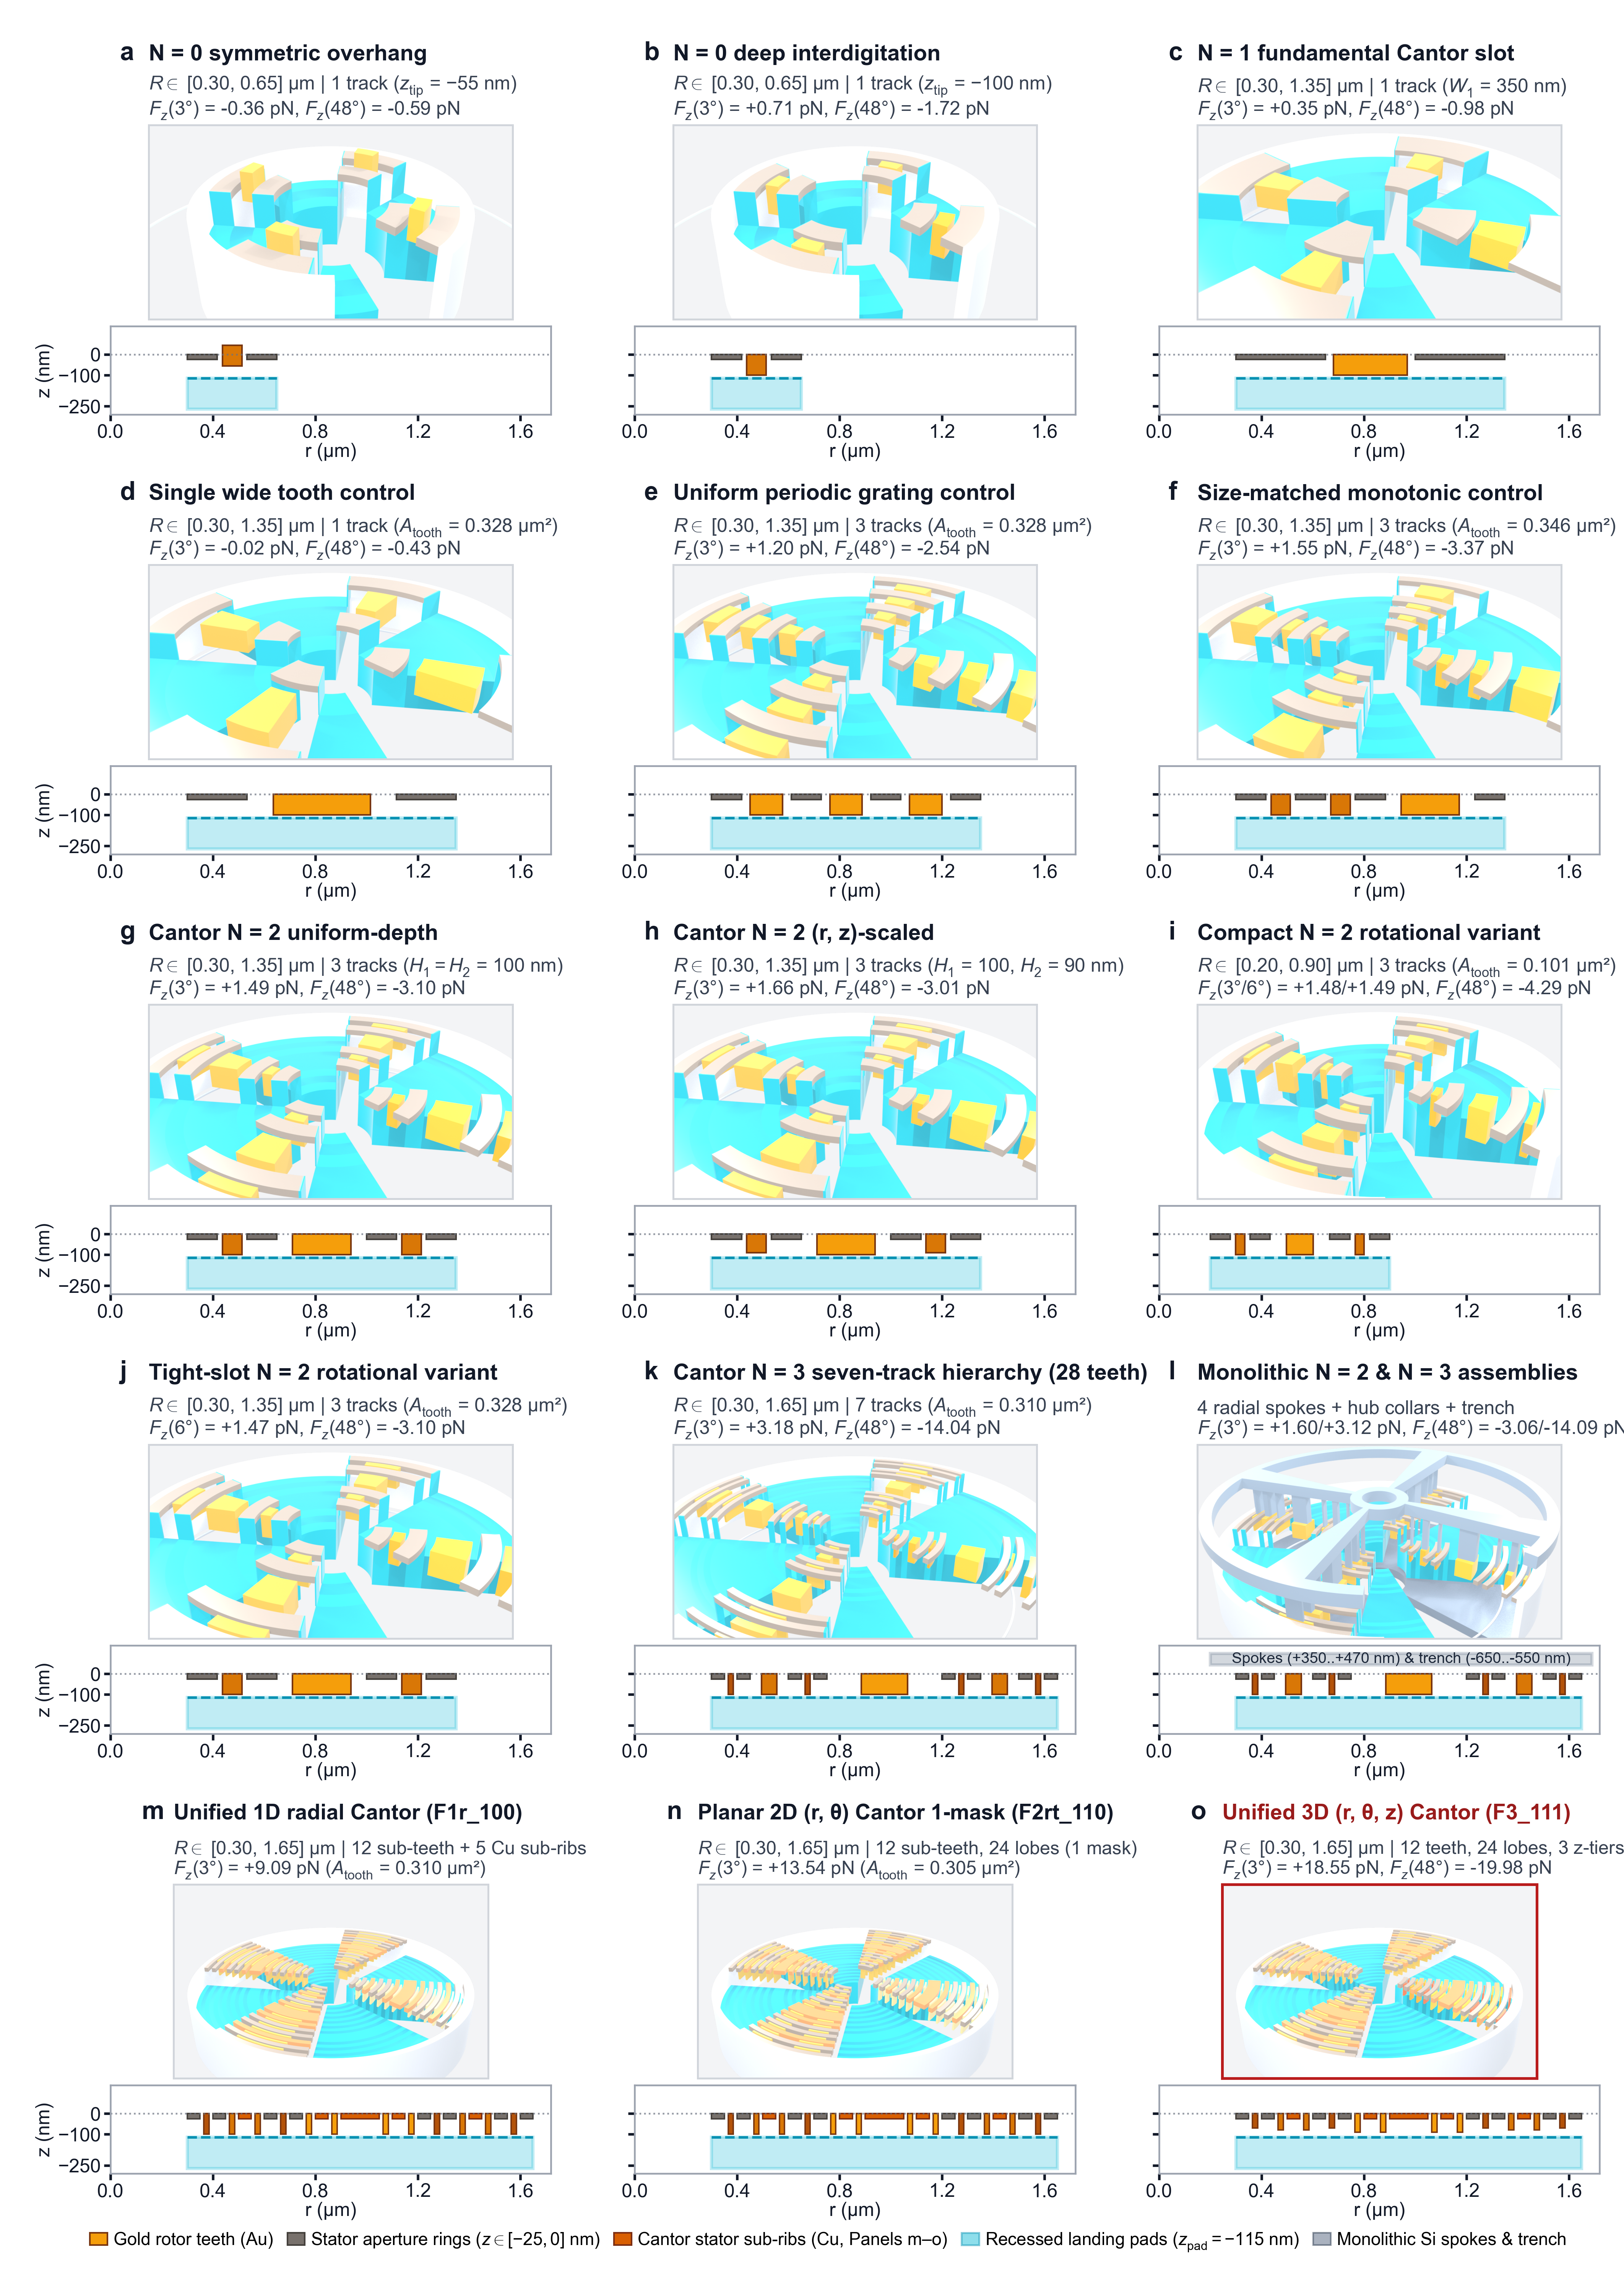
\includegraphics[width=0.95\textwidth]{figures/fig_all_constellations_blender.png}
\caption{\textbf{Three-dimensional geometric atlas across all 12 evaluated cavity constellations in vacuum ($\varepsilon_{\rm bg}=1.0$).} Individual 3D cutaway portraits and radial cross-section $(r, z)$ geometry bars across all 12 constellations: \textbf{a}, $N=0$ symmetric overhang (\texttt{SingleTooth\_Track0}, $z_{\rm tip} = -55\text{ nm}$); \textbf{b}, $N=0$ deep interdigitation (\texttt{SingleTooth\_Track0}, $z_{\rm tip} = -100\text{ nm}$); \textbf{c}, $N=1$ fundamental Cantor slot (\texttt{Fractal\_N1\_FundRing}); \textbf{d}, single wide tooth control (\texttt{Ctrl\_SingleWide}); \textbf{e}, uniform periodic grating control (\texttt{Ctrl\_UniformPeriodic}); \textbf{f}, size-matched monotonic array control (\texttt{Ctrl\_SizeMatched\_Monotonic}); \textbf{g}, uniform-depth $N=2$ Cantor ring (\texttt{Cantor\_N2\_FlatZ}, $H_1 = H_2 = 100\text{ nm}$); \textbf{h}, $(r,z)$-scaled $N=2$ Cantor ring (\texttt{Cantor\_N2\_HybridRZ}, $H_1 = 100\text{ nm}$, $H_2 = 90\text{ nm}$); \textbf{i}, compact $N=2$ rotational variant (\texttt{Rot\_C8\_Compact\_N2}); \textbf{j}, tight-slot $N=2$ rotational variant (\texttt{Rot\_C4\_TightSlot\_N2}); \textbf{k}, third-generation seven-track Cantor ring ($N=3$, \texttt{Fractal\_N3\_Cantor7Track}, $28$ teeth); and \textbf{l}, full-monolithic $N=2$ and $N=3$ structural assemblies incorporating four radial spider spokes, hub collars, and lower substrate isolation trenches.}
\label{fig:all_constellations_blender}
\end{figure*}

\clearpage
% tables/table_fractal_geometry_control.tex — Extended Data Table 1
\begin{table*}[!htbp]
\centering
\footnotesize
\renewcommand{\arraystretch}{0.92}
\caption{\textbf{Three-dimensional fractal geometry control across all evaluated cavity constellations and matched $N=2$ and $N=3$ control families in true vacuum ($\varepsilon_{\rm bg}=1.0$).} Radial span $R \in [R_{\rm min}, R_{\rm max}]$, concentric track/sub-slot count, active rotor tooth planform area $A_{\rm tooth}$, edge perimeter $P_{\rm edge}$, disengaged open-slot axial force $F_z(\theta_{\rm off})$, open-slot area force density $F_z(\theta_{\rm off})/A_{\rm tooth}$, open-slot perimeter force density $F_z(\theta_{\rm off})/P_{\rm edge}$, and engaged landing-pad axial force $F_z(48^\circ)$ evaluated on the matched \texttt{Standard} 3D Vector-Dyadic BEM mesh ($656$ panels for $N=0,1$; $\RotCfourTightslotNtwoStandardThetaZerozerosixpzeroPanelCount{}$ panels for $N=2$ and 3-track controls; $\RotConezeroFractalNthreeStandardThetaZerozerothreepzeroPanelCount{}$ panels for 7-track $N=3$ controls; $6{,}784$ panels across four $90^\circ$ sectors for 12-sub-tooth 3D recursive $N=3$ architectures).}
\label{tab:fractal_geometry_control}
\resizebox{\textwidth}{!}{%
\begin{tabular}{llccccrrrrr}
\toprule
Constellation & $N$ / role & $R$ ($\mu$m) & Tracks / Sub-slots & $A_{\rm tooth}$ ($\mu$m$^2$) & $P_{\rm edge}$ ($\mu$m) & $\theta_{\rm off}$ (deg) & $F_z(\theta_{\rm off})$ (pN) & $F_z/A_{\rm tooth}$ (pN\,$\mu$m$^{-2}$) & $F_z/P_{\rm edge}$ (pN\,$\mu$m$^{-1}$) & $F_z(48^\circ)$ (pN) \\
\midrule
\texttt{SingleTooth-Track0} (overhang) & 0 ($z_{\rm tip}=-55\text{ nm}$) & $[\SingletoothTrackzeroRInUm{}, \SingletoothTrackzeroROutUm{}]$ & 1 / 1 & --- & --- & 3 & \SingletoothTrackzeroOverhangBemThetathreeFZPn{} & --- & --- & \SteponeSingleToothZtipZerozeroonetwoFZPn{} \\
\texttt{SingleTooth-Track0} & 0 ($z_{\rm tip}=-100\text{ nm}$) & $[\SingletoothTrackzeroRInUm{}, \SingletoothTrackzeroROutUm{}]$ & 1 / 1 & --- & --- & 3 & \SingletoothTrackzeroBemThetathreeFZPn{} & --- & --- & \SingletoothTrackzeroBemThetafoureightFZPn{} \\
\texttt{Fractal-N1-FundRing} & 1 (fundamental) & $[\FractalNoneFundringRInUm{}, \FractalNoneFundringROutUm{}]$ & 1 / 1 & --- & --- & 3 & \FractalNoneFundringBemThetathreeFZPn{} & --- & --- & \FractalNoneFundringBemThetafoureightFZPn{} \\
\texttt{Ctrl-SingleWide} & 2 (ctrl, 1 trk) & $[0.30, 1.35]$ & 1 / 1 & \NatureCtrlSinglewideFullToothPlanformAreaUmtwo{} & \NatureCtrlSinglewideFullToothPlanformPerimeterUm{} & 3 & \NatureCtrlSinglewideFRepPn{} & \NatureCtrlSinglewideFRepPnPerToothAreaUmtwo{} & \NatureCtrlSinglewideFRepPnPerToothPerimeterUm{} & \NatureCtrlSinglewideFAttPn{} \\
\texttt{Ctrl-UniformPeriodic} & 2 (ctrl, 3 trk) & $[0.30, 1.35]$ & 3 / 3 & \NatureCtrlUniformperiodicFullToothPlanformAreaUmtwo{} & \NatureCtrlUniformperiodicFullToothPlanformPerimeterUm{} & 3 & \NatureCtrlUniformperiodicFRepPn{} & \NatureCtrlUniformperiodicFRepPnPerToothAreaUmtwo{} & \NatureCtrlUniformperiodicFRepPnPerToothPerimeterUm{} & \NatureCtrlUniformperiodicFAttPn{} \\
\texttt{Ctrl-SizeMatched-Monotonic} & 2 (ctrl, 3 trk) & $[0.30, 1.35]$ & 3 / 3 & \NatureCtrlSizematchedMonotonicFullToothPlanformAreaUmtwo{} & \NatureCtrlSizematchedMonotonicFullToothPlanformPerimeterUm{} & 3 & \NatureCtrlSizematchedMonotonicFRepPn{} & \NatureCtrlSizematchedMonotonicFRepPnPerToothAreaUmtwo{} & \NatureCtrlSizematchedMonotonicFRepPnPerToothPerimeterUm{} & \NatureCtrlSizematchedMonotonicFAttPn{} \\
\texttt{Cantor-N2-TrueRZ} & 2 ($H_2=H_1/3$) & $[0.30, 1.35]$ & 3 / 3 & \NatureCantorNtwoTruerzFullToothPlanformAreaUmtwo{} & \NatureCantorNtwoTruerzFullToothPlanformPerimeterUm{} & 3 & \NatureCantorNtwoTruerzFRepPn{} & \NatureCantorNtwoTruerzFRepPnPerToothAreaUmtwo{} & \NatureCantorNtwoTruerzFRepPnPerToothPerimeterUm{} & \NatureCantorNtwoTruerzFAttPn{} \\
\texttt{Cantor-N2-FlatZ} & 2 (flat-$z$) & $[0.30, 1.35]$ & 3 / 3 & \NatureCantorNtwoFlatzFullToothPlanformAreaUmtwo{} & \NatureCantorNtwoFlatzFullToothPlanformPerimeterUm{} & 3 & \NatureCantorNtwoFlatzFRepPn{} & \NatureCantorNtwoFlatzFRepPnPerToothAreaUmtwo{} & \NatureCantorNtwoFlatzFRepPnPerToothPerimeterUm{} & \NatureCantorNtwoFlatzFAttPn{} \\
\texttt{Cantor-N2-HybridRZ} & 2 ($(r,z)$-scaled) & $[0.30, 1.35]$ & 3 / 3 & \NatureCantorNtwoHybridrzFullToothPlanformAreaUmtwo{} & \NatureCantorNtwoHybridrzFullToothPlanformPerimeterUm{} & 3 & \NatureCantorNtwoHybridrzFRepPn{} & \NatureCantorNtwoHybridrzFRepPnPerToothAreaUmtwo{} & \NatureCantorNtwoHybridrzFRepPnPerToothPerimeterUm{} & \NatureCantorNtwoHybridrzFAttPn{} \\
\texttt{Compact-N2} & 2 (compact) & $[0.20, 0.90]$ & 3 / 3 & \NatureRotCeightCompactNtwoFullToothPlanformAreaUmtwo{} & \NatureRotCeightCompactNtwoFullToothPlanformPerimeterUm{} & 3 / 6 & \NatureRotCeightCompactNtwoFRepPn{} / \RotCeightCompactNtwoStandardThetaZerozerosixpzeroVectorDyadicFZPn{} & \NatureRotCeightCompactNtwoFRepPnPerToothAreaUmtwo{} & \NatureRotCeightCompactNtwoFRepPnPerToothPerimeterUm{} & \NatureRotCeightCompactNtwoFAttPn{} \\
\texttt{TightSlot-N2} & 2 (tight-slot) & $[0.30, 1.35]$ & 3 / 3 & \RotCfourTightslotNtwoHighThetaZerofoureightpzeroPolarOverlapUmtwo{} & --- & 6 & \RotCfourTightslotNtwoStandardThetaZerozerosixpzeroVectorDyadicFZPn{} & --- & --- & \RotCfourTightslotNtwoThetaFoureightStepEightFNetPn{} \\
\texttt{Ctrl-N3-Uniform7Track} & 3 (ctrl, 7 trk) & $[\FractalNthreeCantorseventrackRInUm{}, \FractalNthreeCantorseventrackROutUm{}]$ & 7 / 7 & \NatureCtrlNthreeUniformseventrackFullToothPlanformAreaUmtwo{} & \NatureCtrlNthreeUniformseventrackFullToothPlanformPerimeterUm{} & 3 & \NatureCtrlNthreeUniformseventrackFRepPn{} & \NatureCtrlNthreeUniformseventrackFRepPnPerToothAreaUmtwo{} & \NatureCtrlNthreeUniformseventrackFRepPnPerToothPerimeterUm{} & \NatureCtrlNthreeUniformseventrackFAttPn{} \\
\texttt{Ctrl-N3-Monotonic7Track} & 3 (ctrl, 7 trk) & $[\FractalNthreeCantorseventrackRInUm{}, \FractalNthreeCantorseventrackROutUm{}]$ & 7 / 7 & \NatureCtrlNthreeMonotonicseventrackFullToothPlanformAreaUmtwo{} & \NatureCtrlNthreeMonotonicseventrackFullToothPlanformPerimeterUm{} & 3 & \NatureCtrlNthreeMonotonicseventrackFRepPn{} & \NatureCtrlNthreeMonotonicseventrackFRepPnPerToothAreaUmtwo{} & \NatureCtrlNthreeMonotonicseventrackFRepPnPerToothPerimeterUm{} & \NatureCtrlNthreeMonotonicseventrackFAttPn{} \\
\texttt{Ctrl-N3-Shuffled7Track} & 3 (ctrl, 7 trk) & $[\FractalNthreeCantorseventrackRInUm{}, \FractalNthreeCantorseventrackROutUm{}]$ & 7 / 7 & \NatureCtrlNthreeShuffledseventrackFullToothPlanformAreaUmtwo{} & \NatureCtrlNthreeShuffledseventrackFullToothPlanformPerimeterUm{} & 3 & \NatureCtrlNthreeShuffledseventrackFRepPn{} & \NatureCtrlNthreeShuffledseventrackFRepPnPerToothAreaUmtwo{} & \NatureCtrlNthreeShuffledseventrackFRepPnPerToothPerimeterUm{} & \NatureCtrlNthreeShuffledseventrackFAttPn{} \\
\texttt{Cantor-N3-7Track} (\texttt{F0-000}) & 3 ($u=(0,0,0)$) & $[\FractalNthreeCantorseventrackRInUm{}, \FractalNthreeCantorseventrackROutUm{}]$ & 7 / 7 & \NatureFractalNthreeCantorseventrackFullToothPlanformAreaUmtwo{} & \NatureFractalNthreeCantorseventrackFullToothPlanformPerimeterUm{} & 3 & \NatureFractalNthreeCantorseventrackFRepPn{} & \NatureFractalNthreeCantorseventrackFRepPnPerToothAreaUmtwo{} & \NatureFractalNthreeCantorseventrackFRepPnPerToothPerimeterUm{} & \NatureFractalNthreeCantorseventrackFAttPn{} \\
\texttt{F1r-100} (\texttt{Cantor-100-RadialOnly}) & 3 ($u=(1,0,0)$) & $[\FractalNthreeCantorseventrackRInUm{}, \FractalNthreeCantorseventrackROutUm{}]$ & 7 / 12 & \roundfour{\NthreeUnithreedFonezerozeroRAreaUmtwo} & --- & 3 & $+\roundfour{\NthreeUnithreedFonezerozeroRFzPn}$ & $+\roundtwo{\NthreeUnithreedFonezerozeroRFa}$ & --- & --- \\
\texttt{F2rt-110} (\texttt{Cantor-110-Planar1Mask}) & 3 ($u=(1,1,0)$) & $[\FractalNthreeCantorseventrackRInUm{}, \FractalNthreeCantorseventrackROutUm{}]$ & 7 / 12 & \roundfour{\NthreeUnithreedFoneonezeroRthetaPlanarAreaUmtwo} & --- & 3 & $+\roundfour{\NthreeUnithreedFoneonezeroRthetaPlanarFzPn}$ & $+\roundtwo{\NthreeUnithreedFoneonezeroRthetaPlanarFa}$ & --- & --- \\
\textbf{\texttt{F3-111}} (\textbf{\texttt{Cantor-111-Unified3D}}) & $\mathbf{3\ (u=(1,1,1))}$ & $[\FractalNthreeCantorseventrackRInUm{}, \FractalNthreeCantorseventrackROutUm{}]$ & $\mathbf{7 / 12}$ & \textbf{\roundfour{\NthreeUnithreedFoneoneoneUnifiedAreaUmtwo}} & --- & $\mathbf{3}$ & $\mathbf{+\roundfour{\NthreeUnithreedFoneoneoneUnifiedFzPn}}$ & $\mathbf{+\roundtwo{\NthreeUnithreedFoneoneoneUnifiedFa}}$ & --- & $\mathbf{\roundfour{\NthreeUnithreedFoneoneoneUnifiedThetafoureightFzPn}}$ \\
\texttt{Monolithic-N2} & 2 (monolithic) & $[0.30, 1.35]$ & 3 / 3 & \NatureCantorNtwoHybridrzFullToothPlanformAreaUmtwo{} & \NatureCantorNtwoHybridrzFullToothPlanformPerimeterUm{} & 3 & \CantorNtwoHybridrzBemMonolithicThetathreeFZPn{} & --- & --- & \CantorNtwoHybridrzBemMonolithicThetafoureightFZPn{} \\
\texttt{Monolithic-N3} & 3 (monolithic) & $[\FractalNthreeCantorseventrackRInUm{}, \FractalNthreeCantorseventrackROutUm{}]$ & 7 / 7 & \NatureFractalNthreeCantorseventrackFullToothPlanformAreaUmtwo{} & \NatureFractalNthreeCantorseventrackFullToothPlanformPerimeterUm{} & 3 & \FractalNthreeCantorseventrackBemMonolithicThetathreeFZPn{} & --- & --- & \FractalNthreeCantorseventrackBemMonolithicThetafoureightFZPn{} \\
\botrule
\end{tabular}%
}
\end{table*}

% tables/table_quantum_clutch.tex — Extended Data Table 3
\begin{table*}[!htbp]
\centering
\footnotesize
\renewcommand{\arraystretch}{0.88}
\caption{\textbf{Multi-resolution BEM convergence, corner-rounding regularization ($r_{\rm edge}=5\text{ nm}$), and qualitative 4-pass FDTD sign checks of rotational switching in vacuum ($\varepsilon_{\rm bg}=1.0$).} Axial Casimir forces $F_z$ (in pN) across Standard ($\RotCfourTightslotNtwoStandardThetaZerozerosixpzeroPanelCount{}$ panels for $N=2$; $\RotConezeroFractalNthreeStandardThetaZerozerothreepzeroPanelCount{}$ for 7-track $N=3$; $6{,}784$ panels across 4 sectors for 12-sub-tooth 3D recursive $N=3$), High ($\RotCfourTightslotNtwoHighThetaZerozerosixpzeroPanelCount{}$ panels for $N=2$; $\RotConezeroFractalNthreeHighThetaZerozerothreepzeroPanelCount{}$ for $N=3$), and Ultra-High ($\RotCfourTightslotNtwoUltraHighThetaZerozerosixpzeroPanelCount{}$ panels for $N=2$) surface discretizations in 3D Vector-Dyadic BEM, alongside independent qualitative sign checks from diagnostic 3D Scalar-Yukawa BEM (High) and 4-pass inclusion--exclusion 3D FDTD MEEP ($R=50$, $\Delta x = 20\text{ nm}$). Each 4-pass FDTD evaluation integrates $\FdtdMomentsPerToothPerPass{}$ DCT moments per tooth per pass across $\FdtdInclusionExclusionPasses{}$ passes ($\NaturemeeptaskzerozerofourMomentsPerConfig{}/\NaturemeeptaskzerozerofourTotalMoments{}$ per-pass/total moments for $N=2$ and $\RotConezeroFractalNthreeMomentsPerConfig{}/\RotConezeroFractalNthreeTotalMoments{}$ for $N=3$).}
\label{tab:quantum_clutch}
\resizebox{\textwidth}{!}{%
\begin{tabular}{lcrrrrr}
\toprule
Switch constellation & $\theta$ (deg) & 3D BEM Std (pN) & 3D BEM High (pN) & 3D BEM Ultra-High (pN) & Diagnostic Scalar High (pN) & Qualitative 4-Pass FDTD $R=50$ (pN)$^{\dagger}$ \\
\midrule
\texttt{Cantor-N2-HybridRZ} & 3 & $+\CantorNtwoHybridrzBemStdFZPn{}$ & $+\CantorNtwoHybridrzBemHighFZPn{}$ & $+\CantorNtwoHybridrzBemUltraFZPn{}$ & $+\CantorNtwoHybridrzBemScalarStdThetathreeFZPn{}^{\ast}$ & $+\CantorNtwoHybridrzMeepRfivezeroFZPn{}$ \\
\texttt{Cantor-N2-HybridRZ} ($r_{\rm edge}=5\text{ nm}$) & 3 & $+\CantorNtwoHybridrzBemRfiveNmStdFZPn{}$ & $+\CantorNtwoHybridrzBemRfiveNmHighFZPn{}$ & $+\CantorNtwoHybridrzBemRfiveNmUltraFZPn{}$ & --- & --- \\
\texttt{Cantor-N2-HybridRZ} & 48 & \CantorNtwoHybridrzBemThetafoureightFZPn{} & \CantorNtwoHybridrzBemHighThetafoureightFZPn{} & \CantorNtwoHybridrzBemUltraThetafoureightFZPn{} & $\CantorNtwoHybridrzBemScalarStdThetafoureightFZPn{}^{\ast}$ & \CantorNtwoHybridrzMeepThetafoureightFZPn{} \\
\texttt{Cantor-N2-FlatZ} & 3 & $+\CantorNtwoFlatzBemThetathreeFZPn{}$ & --- & --- & --- & $+\CantorNtwoFlatzMeepThetathreeFZPn{}$ \\
\texttt{Cantor-N2-FlatZ} & 48 & \CantorNtwoFlatzBemThetafoureightFZPn{} & --- & --- & --- & \CantorNtwoFlatzMeepThetafoureightFZPn{} \\
\texttt{Ctrl-UniformPeriodic} & 3 & $+\CtrlUniformperiodicBemThetathreeFZPn{}$ & $+\CtrlUniformperiodicBemHighThetathreeFZPn{}$ & $+\CtrlUniformperiodicBemUltraThetathreeFZPn{}$ & --- & $+\CtrlUniformperiodicMeepThetathreeFZPn{}$ \\
\texttt{Ctrl-UniformPeriodic} ($r_{\rm edge}=5\text{ nm}$) & 3 & $+\CtrlUniformperiodicBemRfiveNmStdFZPn{}$ & $+\CtrlUniformperiodicBemRfiveNmHighFZPn{}$ & $+\CtrlUniformperiodicBemRfiveNmUltraFZPn{}$ & --- & --- \\
\texttt{Ctrl-UniformPeriodic} & 48 & \CtrlUniformperiodicBemThetafoureightFZPn{} & --- & --- & --- & \CtrlUniformperiodicMeepThetafoureightFZPn{} \\
\texttt{Compact-N2} & 0 & $+\RotCeightCompactNtwoThetaZeroStepNineFNetPn{}$ & --- & --- & --- & $+\RotCeightCompactNtwoMeepThetazeroFZPn{}$ \\
\texttt{Compact-N2} & 6 & $+\RotCeightCompactNtwoStandardThetaZerozerosixpzeroVectorDyadicFZPn{}$ & $+\RotCeightCompactNtwoHighThetaZerozerosixpzeroVectorDyadicFZPn{}$ & $+\RotCeightCompactNtwoUltraHighThetaZerozerosixpzeroVectorDyadicFZPn{}$ & $+\RotCeightCompactNtwoHighThetaZerozerosixpzeroScalarYukawaFZPn{}$ & $+\RotCeightCompactNtwoMeepThetasixFZPn{}$ \\
\texttt{Compact-N2} & 18 & \RotCeightCompactNtwoStandardThetaZerooneeightpzeroVectorDyadicFZPn{} & \RotCeightCompactNtwoHighThetaZerooneeightpzeroVectorDyadicFZPn{} & \RotCeightCompactNtwoUltraHighThetaZerooneeightpzeroVectorDyadicFZPn{} & \RotCeightCompactNtwoHighThetaZerooneeightpzeroScalarYukawaFZPn{} & \RotCeightCompactNtwoMeepThetaoneeightFZPn{} \\
\texttt{Compact-N2} & 48 & \RotCeightCompactNtwoStandardThetaZerofoureightpzeroVectorDyadicFZPn{} & \RotCeightCompactNtwoHighThetaZerofoureightpzeroVectorDyadicFZPn{} & \RotCeightCompactNtwoUltraHighThetaZerofoureightpzeroVectorDyadicFZPn{} & \RotCeightCompactNtwoHighThetaZerofoureightpzeroScalarYukawaFZPn{} & \RotCeightCompactNtwoMeepThetafoureightFZPn{} \\
\texttt{TightSlot-N2} & 0 & $+\RotCfourTightslotNtwoThetaZeroStepZeroFNetPn{}$ & --- & --- & --- & $+\RotCfourTightslotNtwoMeepThetazeroFZPn{}$ \\
\texttt{TightSlot-N2} & 6 & $+\RotCfourTightslotNtwoStandardThetaZerozerosixpzeroVectorDyadicFZPn{}$ & $+\RotCfourTightslotNtwoHighThetaZerozerosixpzeroVectorDyadicFZPn{}$ & $+\RotCfourTightslotNtwoUltraHighThetaZerozerosixpzeroVectorDyadicFZPn{}$ & $+\RotCfourTightslotNtwoHighThetaZerozerosixpzeroScalarYukawaFZPn{}$ & $+\RotCfourTightslotNtwoMeepThetasixFZPn{}$ \\
\texttt{TightSlot-N2} & 12 & $+\RotCfourTightslotNtwoThetaOnetwoStepTwoFNetPn{}$ & --- & --- & --- & $+\RotCfourTightslotNtwoMeepThetaonetwoFZPn{}$ \\
\texttt{TightSlot-N2} & 18 & \RotCfourTightslotNtwoThetaOneeightStepThreeFNetPn{} & \RotCfourTightslotNtwoHighThetaZerooneeightpzeroVectorDyadicFZPn{} & \RotCfourTightslotNtwoUltraHighThetaZerooneeightpzeroVectorDyadicFZPn{} & \RotCfourTightslotNtwoHighThetaZerooneeightpzeroScalarYukawaFZPn{} & \RotCfourTightslotNtwoMeepThetaoneeightFZPn{} \\
\texttt{TightSlot-N2} & 48 & \RotCfourTightslotNtwoThetaFoureightStepEightFNetPn{} & \RotCfourTightslotNtwoHighThetaZerofoureightpzeroVectorDyadicFZPn{} & \RotCfourTightslotNtwoUltraHighThetaZerofoureightpzeroVectorDyadicFZPn{} & \RotCfourTightslotNtwoHighThetaZerofoureightpzeroScalarYukawaFZPn{} & \RotCfourTightslotNtwoMeepThetafoureightFZPn{} \\
\texttt{Cantor-N3-7Track} (\texttt{F0-000}) & 3 & $+\RotConezeroFractalNthreeStandardThetaZerozerothreepzeroVectorDyadicFZPn{}$ & $+\RotConezeroFractalNthreeHighThetaZerozerothreepzeroVectorDyadicFZPn{}$ & --- & $+\RotConezeroFractalNthreeHighThetaZerozerothreepzeroScalarYukawaFZPn{}$ & $+\RotConezeroFractalNthreeMeepThetathreeFZPn{}$ \\
\texttt{Cantor-N3-7Track} (\texttt{F0-000}) & 21 & \RotConezeroFractalNthreeStandardThetaZerotwoonepzeroVectorDyadicFZPn{} & \RotConezeroFractalNthreeHighThetaZerotwoonepzeroVectorDyadicFZPn{} & --- & \RotConezeroFractalNthreeHighThetaZerotwoonepzeroScalarYukawaFZPn{} & \RotConezeroFractalNthreeMeepThetatwooneFZPn{} \\
\texttt{Cantor-N3-7Track} (\texttt{F0-000}) & 48 & \RotConezeroFractalNthreeStandardThetaZerofoureightpzeroVectorDyadicFZPn{} & \RotConezeroFractalNthreeHighThetaZerofoureightpzeroVectorDyadicFZPn{} & --- & \RotConezeroFractalNthreeHighThetaZerofoureightpzeroScalarYukawaFZPn{} & \RotConezeroFractalNthreeMeepThetafoureightFZPn{} \\
\midrule
\texttt{F2rt-110} (\texttt{Cantor-110-Planar1Mask}) & 3 & $+\roundfour{\NthreeUnithreedFoneonezeroRthetaPlanarFzPn}$ & --- & --- & --- & --- \\
\textbf{\texttt{F3-111}} (\textbf{\texttt{Cantor-111-Unified3D}}) & $\mathbf{3}$ & $\mathbf{+\roundfour{\NthreeUnithreedFoneoneoneUnifiedFzPn}}$ & --- & --- & --- & --- \\
\textbf{\texttt{F3-111}} ($\mathbf{r_{\rm edge}=5\text{ nm}}$) & $\mathbf{3}$ & $\mathbf{+\roundfour{\NthreeUnithreedFoneoneoneRfivenmFzPn}}$ & --- & --- & --- & --- \\
\texttt{C6-Uni12} ($r_{\rm edge}=5\text{ nm}$) & 3 & $+\roundfour{\NthreeUnithreedCtrlUnionetwoRfivenmFzPn}$ & --- & --- & --- & --- \\
\texttt{C8-Mono12} ($r_{\rm edge}=5\text{ nm}$) & 3 & $+\roundfour{\NthreeUnithreedCtrlMonoonetwoRfivenmFzPn}$ & --- & --- & --- & --- \\
\texttt{C9-Shuf12} ($r_{\rm edge}=5\text{ nm}$) & 3 & $+\roundfour{\NthreeUnithreedCtrlShufonetwoRfivenmFzPn}$ & --- & --- & --- & --- \\
\textbf{\texttt{F3-111}} (\textbf{\texttt{Cantor-111-Unified3D}}) & $\mathbf{21}$ & $\mathbf{+\roundfour{\NthreeUnithreedFoneoneoneUnifiedThetatwooneFzPn}}$ & --- & --- & --- & --- \\
\textbf{\texttt{F3-111}} (\textbf{\texttt{Cantor-111-Unified3D}}) & $\mathbf{48}$ & $\mathbf{\roundfour{\NthreeUnithreedFoneoneoneUnifiedThetafoureightFzPn}}$ & --- & --- & --- & --- \\
\botrule
\end{tabular}%
}
\smallskip
\scriptsize{$^{\ast}$Evaluated on the \texttt{Standard} 3D Scalar-Yukawa BEM mesh for \texttt{Cantor-N2-HybridRZ}. $^{\dagger}$At $R=50$ ($\Delta x = 20\text{ nm}$) with subpixel permittivity averaging disabled (\texttt{eps\_averaging = False}) and $n_{\rm max}=1$ DCT moments per face, the $15\text{ nm}$ clearances span $\sim 1$ Yee voxel and expanding to $n_{\rm max}=2$ shifts the open-slot force by $+\MeepFixedboxRsixzeroNmaxtwoGainPct{}\%$; accordingly, the 4-pass FDTD column serves strictly as an independent qualitative sign check rather than a quantitative validation. For the 12-sub-tooth 3D recursive $N=3$ family (\texttt{F3-111}, \texttt{F2rt-110}, and controls \texttt{C6-Uni12} through \texttt{C10-OutPhase12}), each $90^\circ$ sector is discretized with $768$ rotor panels and $928$ stator panels ($1{,}696$ panels per sector; $6{,}784$ across four sectors) and $24$ identical $90^\circ$ azimuthal lobes per sector.}
\end{table*}

% tables/table_nems_feasibility.tex — Extended Data Table 4
\begin{table*}[!htbp]
\centering
\footnotesize
\renewcommand{\arraystretch}{0.84}
\setlength{\tabcolsep}{4pt}
\caption{\textbf{Room-temperature ($T = \NatureRotCeightCompactNtwoCdToleranceTemperatureK{}\text{ K}$) NEMS mechanical feasibility, discretization-bounded pull-in thresholds, multi-regime $\text{Si}\langle 110\rangle$ flexure stroke scaling, and lithographic tolerances in vacuum ($\varepsilon_{\rm bg}=1.0$).} Comparison of thermal Matsubara dispersion, capacitance-gradient patch-voltage thresholds $V_{\rm crit}$, four-spoke single-crystal $\text{Si}\langle 110\rangle$ suspension designs ($E_Y = \scinum{\NatureRotCeightCompactNtwoLateralStabilityEYPa}\text{ Pa}$) across three operational stroke regimes bounded across (a) Standard sharp-edge BEM ($N_{\rm panels}=\RotCfourTightslotNtwoStandardThetaZerozerosixpzeroPanelCount{}$ for $N=2$; $6{,}784$ for \texttt{F3-111}), (b) $r_{\rm edge}=5\text{ nm}$ rounded-edge BEM ($N_{\rm panels}=\RotCfourTightslotNtwoUltraHighThetaZerozerosixpzeroPanelCount{}$ Ultra-High for $N=2$; Standard per-sub-tooth density for \texttt{F3-111}), and (c) continuum-extrapolated ($N_{\rm panels}\to\infty$) forces, plus EBL corner rounding ($r_{\rm edge}$) and critical-dimension tooth-width biases ($\Delta w_{\rm tooth}$) for \texttt{Cantor-N2-HybridRZ}, \texttt{Compact-N2}, and best-performing \texttt{F3-111}.}
\label{tab:nems_feasibility}
\resizebox{\textwidth}{!}{%
\begin{tabular}{llrrr}
\toprule
Benchmark category & Parameter / operating condition & \texttt{Cantor-N2-HybridRZ} & \texttt{Compact-N2} & \textbf{\texttt{F3-111} (\texttt{Cantor-111})} \\
\midrule
\multirow{3}{*}{Thermal dispersion ($\theta_{\rm off}$ / $48^\circ$)} 
 & Ideal PEC ($T = 0\text{ K}$) $F_z$ (pN) & $+\NatureCantorNtwoHybridrzStepzeroForceZPn{}$ / $\NatureCantorNtwoHybridrzSteponeForceZPn{}$ & $+\NatureRotCeightCompactNtwoSteponesixForceZPn{}$ / $\NatureRotCeightCompactNtwoSteponesevenForceZPn{}$ & --- \\
 & Drude gold ($T = 0\text{ K}$) $F_z$ (pN) & $+\NatureCantorNtwoHybridrzSteptwoForceZPn{}$ / $\NatureCantorNtwoHybridrzStepthreeForceZPn{}$ & $+\NatureRotCeightCompactNtwoSteponeeightForceZPn{}$ / $\NatureRotCeightCompactNtwoSteponenineForceZPn{}$ & $+\roundtwo{\NthreeUnithreedFoneoneoneUnifiedFzPn}$ / $\roundtwo{\NthreeUnithreedFoneoneoneUnifiedThetafoureightFzPn}$ \\
 & Room-temperature Drude gold ($T = \NatureRotCeightCompactNtwoCdToleranceTemperatureK{}\text{ K}$) $F_z$ (pN) & $+\NatureCantorNtwoHybridrzStepfourForceZPn{}$ / $\NatureCantorNtwoHybridrzStepfiveForceZPn{}$ & $+\NatureRotCeightCompactNtwoSteptwozeroForceZPn{}$ / $\NatureRotCeightCompactNtwoSteptwooneForceZPn{}$ & $+\roundtwo{\NatureFthreeOneoneoneFRepThreezerozerokPn}$ / $\roundtwo{\NatureFthreeOneoneoneFEngagedThreezerozerokPn}$ \\
\midrule
\multirow{2}{*}{Electrostatic patch budget} 
 & Mutual-capacitance gradient $|\partial C_{\rm el}/\partial z|$ (pN\,mV$^{-2}$) & \NatureCantorNtwoHybridrzPatchPotentialAbsDcDzPnPerMvtwo{} & \NatureRotCeightCompactNtwoPatchPotentialAbsDcDzPnPerMvtwo{} & $\roundfour{\NatureFthreeOneoneoneAbsDcDzPnPerMvtwo}$ \\
 & Critical RMS voltage $V_{\rm crit}$: (a) Std / (b) $r_{\rm edge}=5\text{ nm}$ / (c) Cont.\ (mV) & \NatureCantorNtwoHybridrzPatchPotentialVCritMv{} / \NatureCantorNtwoHybridrzDiscretizationPullInBoundsRfiveUltraVCritMv{} / \NatureCantorNtwoHybridrzDiscretizationPullInBoundsContinuumVCritMv{} & \NatureRotCeightCompactNtwoPatchPotentialVCritMv{} / \NatureRotCeightCompactNtwoDiscretizationPullInBoundsRfiveUltraVCritMv{} / \NatureRotCeightCompactNtwoDiscretizationPullInBoundsContinuumVCritMv{} & $\roundone{\NatureFthreeOneoneoneVCritMv}$ / $\roundone{\NatureFthreeOneoneoneVCritRfivenmMv}$ / --- \\
\midrule
\multirow{7}{*}{Regime I: Isometric transducer} 
 & Spoke geometry $L_{\rm spoke} \times w_{\rm spoke} \times t_{\rm spoke}$ ($\mu$m$^3$) & $\NatureRotCeightCompactNtwoLateralStabilityLSpokeUm{} \times \NatureRotCeightCompactNtwoLateralStabilityWSpokeUm{} \times \NatureRotCeightCompactNtwoLateralStabilityTSpokeUm{}$ & $\NatureRotCeightCompactNtwoLateralStabilityLSpokeUm{} \times \NatureRotCeightCompactNtwoLateralStabilityWSpokeUm{} \times \NatureRotCeightCompactNtwoLateralStabilityTSpokeUm{}$ & $\NatureRotCeightCompactNtwoLateralStabilityLSpokeUm{} \times \NatureRotCeightCompactNtwoLateralStabilityWSpokeUm{} \times \NatureRotCeightCompactNtwoLateralStabilityTSpokeUm{}$ \\
 & Stiffness $k_{z,\rm mech}$ / $k_{r,\rm mech}$ (pN\,nm$^{-1}$) & \NatureRotCeightCompactNtwoLateralStabilityKZMechPnPerNm{} / \NatureRotCeightCompactNtwoLateralStabilityKRMechPnPerNm{} & \NatureRotCeightCompactNtwoLateralStabilityKZMechPnPerNm{} / \NatureRotCeightCompactNtwoLateralStabilityKRMechPnPerNm{} & \NatureRotCeightCompactNtwoLateralStabilityKZMechPnPerNm{} / \NatureRotCeightCompactNtwoLateralStabilityKRMechPnPerNm{} \\
 & Modal mass $m_{\rm eff}$ (pg) / $f_0$ beam / $f_{0,\rm FEM}$ (kHz) & $\roundtwo{\NatureCantorNtwoHybridrzMEffRegonePg}$ / $\roundone{\NatureCantorNtwoHybridrzResFreqKhz}$ / $\roundone{\NatureCantorNtwoHybridrzFemFreqRegoneKhz}$ & $\roundtwo{\NatureRotCeightCompactNtwoMEffRegonePg}$ / $\roundone{\NatureRotCeightCompactNtwoResFreqKhz}$ / $\roundone{\NatureRotCeightCompactNtwoFemFreqRegoneKhz}$ & $\roundtwo{\NatureFthreeOneoneoneMEffRegonePg}$ / $\roundone{\NatureFthreeOneoneoneFZeroRegoneKhz}$ / $\roundone{\NatureFthreeOneoneoneFemFreqRegoneKhz}$ \\
 & 300 K $\delta z_{\rm th}$ (pm) / $S_F^{1/2}$ ($Q=10^4$, fN\,Hz$^{-1/2}$) / $\mathrm{SNR}(1\text{ s})$ / $\tau_{\rm SNR=100}$ ($\mu$s) & $\roundone{\NatureCantorNtwoHybridrzThermalDzRegimeOnePm}$ / $\roundthree{\NatureCantorNtwoHybridrzSfSqrtRegoneQoneefourFn}$ / $\roundzero{\NatureCantorNtwoHybridrzSnrOneSec}$ / $\roundone{\NatureCantorNtwoHybridrzTauSnronezerozeroRegoneQoneefourUs}$ & $\roundone{\NatureRotCeightCompactNtwoThermalDzRegimeOnePm}$ / $\roundthree{\NatureRotCeightCompactNtwoSfSqrtRegoneQoneefourFn}$ / $\roundzero{\NatureRotCeightCompactNtwoSnrOneSec}$ / $\roundone{\NatureRotCeightCompactNtwoTauSnronezerozeroRegoneQoneefourUs}$ & $\roundone{\NatureCantorNtwoHybridrzThermalDzRegimeOnePm}$ / $\roundthree{\NatureFthreeOneoneoneSFSqrtFnPerRthzQoneefour}$ / $\roundzero{\NatureFthreeOneoneoneSnrOneSecQoneefour}$ / $\roundtwo{\NatureFthreeOneoneoneTauSnronezerozeroRegoneQoneefourUs}$ \\
 & Lateral safety factor / (a) Std vertical pull-in $\text{SF}_z$ & $\NatureCantorNtwoHybridrzLateralStabilityLateralStabilitySafetyFactor{}\times$ / $\NatureCantorNtwoHybridrzLateralStabilityVerticalPullInSafetyFactor{}\times$ & $\NatureRotCeightCompactNtwoLateralStabilityLateralStabilitySafetyFactor{}\times$ / $\NatureRotCeightCompactNtwoLateralStabilityVerticalPullInSafetyFactor{}\times$ & $\roundzero{\NatureFthreeOneoneoneRegoneLateralStabilitySafetyFactor}\times$ / $\roundtwo{\NatureFthreeOneoneoneRegoneVerticalPullInSafetyFactor}\times$ \\
 & Bounded vertical pull-in $\text{SF}_z$: (b) High/Ultra BEM / (c) Continuum & $\NatureCantorNtwoHybridrzDiscretizationPullInBoundsSharpUltraSfPullInRegone{}\times$ / $\NatureCantorNtwoHybridrzDiscretizationPullInBoundsContinuumSfPullInRegone{}\times$ & $\NatureRotCeightCompactNtwoDiscretizationPullInBoundsSharpUltraSfPullInRegone{}\times$ / $\NatureCantorNtwoHybridrzDiscretizationPullInBoundsContinuumSfPullInRegone{}\times$ & --- / --- \\
 & Equilibrium axial deflection $\Delta z(\theta_{\rm off})$ / $\Delta z(48^\circ)$ (nm) & $+\NatureCantorNtwoHybridrzLateralStabilityEquilibriumAxialRepulsiveLiftNm{}$ / $\NatureCantorNtwoHybridrzLateralStabilityEngagedLinearAxialDeflectionNm{}$ & $+\NatureRotCeightCompactNtwoLateralStabilityEquilibriumAxialRepulsiveLiftNm{}$ / $\NatureRotCeightCompactNtwoLateralStabilityEngagedLinearAxialDeflectionNm{}$ & $+\roundfour{\NatureFthreeOneoneoneRegoneEquilibriumAxialRepulsiveLiftNm}$ / $\roundfour{\NatureFthreeOneoneoneRegoneEngagedLinearAxialDeflectionNm}$ \\
\midrule
\multirow{7}{*}{Regime II: Nanometre-stroke} 
 & Spoke geometry $L_{\rm spoke} \times w_{\rm spoke} \times t_{\rm spoke}$ ($\mu$m$^3$) & $\NatureRotCeightCompactNtwoLateralStabilityNmActuatorLSpokeUm{} \times \NatureRotCeightCompactNtwoLateralStabilityNmActuatorWSpokeUm{} \times \NatureRotCeightCompactNtwoLateralStabilityNmActuatorTSpokeUm{}$ & $\NatureRotCeightCompactNtwoLateralStabilityNmActuatorLSpokeUm{} \times \NatureRotCeightCompactNtwoLateralStabilityNmActuatorWSpokeUm{} \times \NatureRotCeightCompactNtwoLateralStabilityNmActuatorTSpokeUm{}$ & $\NatureRotCeightCompactNtwoLateralStabilityNmActuatorLSpokeUm{} \times \NatureRotCeightCompactNtwoLateralStabilityNmActuatorWSpokeUm{} \times \NatureRotCeightCompactNtwoLateralStabilityNmActuatorTSpokeUm{}$ \\
 & Stiffness $k_{z,\rm mech}$ / $k_{r,\rm mech}$ (pN\,nm$^{-1}$) & \NatureRotCeightCompactNtwoLateralStabilityNmActuatorKZMechPnPerNm{} / \NatureRotCeightCompactNtwoLateralStabilityNmActuatorKRMechPnPerNm{} & \NatureRotCeightCompactNtwoLateralStabilityNmActuatorKZMechPnPerNm{} / \NatureRotCeightCompactNtwoLateralStabilityNmActuatorKRMechPnPerNm{} & \NatureRotCeightCompactNtwoLateralStabilityNmActuatorKZMechPnPerNm{} / \NatureRotCeightCompactNtwoLateralStabilityNmActuatorKRMechPnPerNm{} \\
 & Modal mass $m_{\rm eff}$ (pg) / $f_0$ beam / $f_{0,\rm FEM}$ (kHz) & $\roundtwo{\NatureCantorNtwoHybridrzMEffRegtwoPg}$ / $\roundone{\NatureCantorNtwoHybridrzResFreqRegimeTwoKhz}$ / $\roundone{\NatureCantorNtwoHybridrzFemFreqRegtwoKhz}$ & $\roundtwo{\NatureRotCeightCompactNtwoMEffRegtwoPg}$ / $\roundone{\NatureRotCeightCompactNtwoResFreqRegimeTwoKhz}$ / $\roundone{\NatureRotCeightCompactNtwoFemFreqRegtwoKhz}$ & $\roundtwo{\NatureFthreeOneoneoneMEffRegtwoPg}$ / $\roundone{\NatureFthreeOneoneoneFZeroRegtwoKhz}$ / $\roundone{\NatureFthreeOneoneoneFemFreqRegtwoKhz}$ \\
 & 300 K $\delta z_{\rm th}$ (nm) / $S_F^{1/2}$ ($Q=10^4$, fN\,Hz$^{-1/2}$) / $\mathrm{SNR}(1\text{ s})$ / $\tau_{\rm SNR=100}$ ($\mu$s) & $\roundtwo{\NatureCantorNtwoHybridrzThermalDzRegimeTwoNm}$ / $\roundthree{\NatureCantorNtwoHybridrzSfSqrtRegtwoQoneefourFn}$ / $\roundzero{\NatureCantorNtwoHybridrzSnrOneSecRegtwo}$ / $\roundone{\NatureCantorNtwoHybridrzTauSnronezerozeroRegtwoQoneefourUs}$ & $\roundtwo{\NatureRotCeightCompactNtwoThermalDzRegimeTwoNm}$ / $\roundthree{\NatureRotCeightCompactNtwoSfSqrtRegtwoQoneefourFn}$ / $\roundzero{\NatureRotCeightCompactNtwoSnrOneSecRegtwo}$ / $\roundone{\NatureRotCeightCompactNtwoTauSnronezerozeroRegtwoQoneefourUs}$ & $\roundtwo{\NatureCantorNtwoHybridrzThermalDzRegimeTwoNm}$ / --- / $\roundzero{\NatureFthreeOneoneoneSnrOneSecRegtwoQoneefour}$ / $\roundtwo{\NatureFthreeOneoneoneTauSnronezerozeroRegtwoQoneefourUs}$ \\
 & Lateral safety factor / (a) Std vertical pull-in $\text{SF}_z$ & $\NatureCantorNtwoHybridrzLateralStabilityNmActuatorLateralSafetyFactor{}\times$ / $\NatureCantorNtwoHybridrzLateralStabilityNmActuatorVerticalPullInSafetyFactor{}\times$ & $\NatureRotCeightCompactNtwoLateralStabilityNmActuatorLateralSafetyFactor{}\times$ / $\NatureRotCeightCompactNtwoLateralStabilityNmActuatorVerticalPullInSafetyFactor{}\times$ & $\roundtwo{\NatureFthreeOneoneoneRegtwoLateralStabilitySafetyFactor}\times$ / $\roundthree{\NatureFthreeOneoneoneRegtwoVerticalPullInSafetyFactor}\times$ \\
 & Bounded vertical pull-in $\text{SF}_z$: (b) High/Ultra BEM / (c) Continuum & $\NatureCantorNtwoHybridrzDiscretizationPullInBoundsSharpUltraSfPullInRegtwo{}\times$ / $\NatureCantorNtwoHybridrzDiscretizationPullInBoundsContinuumSfPullInRegtwo{}\times$ & $\NatureRotCeightCompactNtwoDiscretizationPullInBoundsSharpUltraSfPullInRegtwo{}\times$ / $\NatureCantorNtwoHybridrzDiscretizationPullInBoundsContinuumSfPullInRegtwo{}\times$ & --- / --- \\
 & Self-consistent repulsive lift (a) Std / (b) $r_{\rm edge}=5\text{ nm}$ / stroke (nm) & $+\NatureCantorNtwoHybridrzLateralStabilityNmActuatorBasinEqLiftNm{}$ / $+\NatureCantorNtwoHybridrzDiscretizationPullInBoundsRfiveUltraLiftRegtwoNm{}$ / $\NatureCantorNtwoHybridrzLateralStabilityNmActuatorPeakToPeakStrokeNm{}$ & $+\NatureRotCeightCompactNtwoLateralStabilityNmActuatorBasinEqLiftNm{}$ / $+\NatureRotCeightCompactNtwoDiscretizationPullInBoundsRfiveUltraLiftRegtwoNm{}$ / $\NatureRotCeightCompactNtwoLateralStabilityNmActuatorPeakToPeakStrokeNm{}$ & $+\roundtwo{\NatureFthreeOneoneoneRegtwoSelfConsistentBasinRepulsiveLiftNm}$ / $+\roundtwo{\NatureFthreeOneoneoneRegtwoRfivenmBasinLiftNm}$ / $\roundtwo{\NatureFthreeOneoneoneRegtwoPeakToPeakLinearStrokeNm}$ \\
\midrule
\multirow{6}{*}{Regime III: Contact-release actuator} 
 & Compact $50\text{ nm}$ SOI spoke $L_{\rm spoke} \times w_{\rm spoke} \times t_{\rm spoke}$ ($\mu$m$^3$) & $\NatureRotCeightCompactNtwoLateralStabilityCompactClutchLSpokeUm{} \times \NatureRotCeightCompactNtwoLateralStabilityCompactClutchWSpokeUm{} \times \NatureRotCeightCompactNtwoLateralStabilityCompactClutchTSpokeUm{}$ & $\NatureRotCeightCompactNtwoLateralStabilityCompactClutchLSpokeUm{} \times \NatureRotCeightCompactNtwoLateralStabilityCompactClutchWSpokeUm{} \times \NatureRotCeightCompactNtwoLateralStabilityCompactClutchTSpokeUm{}$ & $\NatureRotCeightCompactNtwoLateralStabilityCompactClutchLSpokeUm{} \times \NatureRotCeightCompactNtwoLateralStabilityCompactClutchWSpokeUm{} \times \NatureRotCeightCompactNtwoLateralStabilityCompactClutchTSpokeUm{}$ \\
 & Stiffness $k_{z,\rm mech}$ / $k_{r,\rm mech}$ (pN\,nm$^{-1}$) & \NatureRotCeightCompactNtwoLateralStabilityCompactClutchKZMechPnPerNm{} / \NatureRotCeightCompactNtwoLateralStabilityCompactClutchKRMechPnPerNm{} & \NatureRotCeightCompactNtwoLateralStabilityCompactClutchKZMechPnPerNm{} / \NatureRotCeightCompactNtwoLateralStabilityCompactClutchKRMechPnPerNm{} & \NatureRotCeightCompactNtwoLateralStabilityCompactClutchKZMechPnPerNm{} / \NatureRotCeightCompactNtwoLateralStabilityCompactClutchKRMechPnPerNm{} \\
 & Modal mass $m_{\rm eff}$ (pg) / $f_0$ beam / $f_{0,\rm FEM}$ (kHz) & $\roundtwo{\NatureCantorNtwoHybridrzMEffRegthreePg}$ / $\roundone{\NatureCantorNtwoHybridrzResFreqRegimeThreeKhz}$ / $\roundone{\NatureCantorNtwoHybridrzFemFreqRegthreeKhz}$ & $\roundtwo{\NatureRotCeightCompactNtwoMEffRegthreePg}$ / $\roundone{\NatureRotCeightCompactNtwoResFreqRegimeThreeKhz}$ / $\roundone{\NatureRotCeightCompactNtwoFemFreqRegthreeKhz}$ & $\roundtwo{\NatureFthreeOneoneoneMEffRegthreePg}$ / $\roundone{\NatureFthreeOneoneoneFZeroRegthreeKhz}$ / $\roundone{\NatureFthreeOneoneoneFemFreqRegthreeKhz}$ \\
 & 300 K $\delta z_{\rm th}$ (nm) / $S_F^{1/2}$ ($Q=10^4$, fN\,Hz$^{-1/2}$) / $\mathrm{SNR}(1\text{ s})$ / $\tau_{\rm SNR=100}$ ($\mu$s) & $\roundtwo{\NatureCantorNtwoHybridrzThermalDzRegimeThreeNm}$ / $\roundthree{\NatureCantorNtwoHybridrzSfSqrtRegthreeQoneefourFn}$ / $\roundzero{\NatureCantorNtwoHybridrzSnrOneSecRegthree}$ / $\roundone{\NatureCantorNtwoHybridrzTauSnronezerozeroRegthreeQoneefourUs}$ & $\roundtwo{\NatureRotCeightCompactNtwoThermalDzRegimeThreeNm}$ / $\roundthree{\NatureRotCeightCompactNtwoSfSqrtRegthreeQoneefourFn}$ / $\roundzero{\NatureRotCeightCompactNtwoSnrOneSecRegthree}$ / $\roundone{\NatureRotCeightCompactNtwoTauSnronezerozeroRegthreeQoneefourUs}$ & $\roundtwo{\NatureCantorNtwoHybridrzThermalDzRegimeThreeNm}$ / --- / $\roundzero{\NatureFthreeOneoneoneSnrOneSecRegthreeQoneefour}$ / $\roundtwo{\NatureFthreeOneoneoneTauSnronezerozeroRegthreeQoneefourUs}$ \\
 & Lateral safety factor / unlatching lift (a) Std / (b) $r_{\rm edge}=5\text{ nm}$ (nm) & $\NatureCantorNtwoHybridrzLateralStabilityCompactClutchLateralSafetyFactor{}\times$ / $+\NatureCantorNtwoHybridrzLateralStabilityCompactClutchBasinEqLiftNm{}$ / $+\NatureCantorNtwoHybridrzDiscretizationPullInBoundsRfiveUltraLiftRegthreeNm{}$ & $\NatureRotCeightCompactNtwoLateralStabilityCompactClutchLateralSafetyFactor{}\times$ / $+\NatureRotCeightCompactNtwoLateralStabilityCompactClutchBasinEqLiftNm{}$ / $+\NatureRotCeightCompactNtwoDiscretizationPullInBoundsRfiveUltraLiftRegthreeNm{}$ & $\roundtwo{\NatureFthreeOneoneoneRegthreeLateralStabilitySafetyFactor}\times$ / $+\roundtwo{\NatureFthreeOneoneoneRegthreeSelfConsistentBasinRepulsiveLiftNm}$ / $+\roundtwo{\NatureFthreeOneoneoneRegthreeRfivenmBasinLiftNm}$ \\
 & Bounded vertical pull-in $\text{SF}_z$: (a) Std / (b) High/Ultra BEM / (c) Cont. & $\NatureCantorNtwoHybridrzDiscretizationPullInBoundsStdSfPullInRegthree{}\times$ / $\NatureCantorNtwoHybridrzDiscretizationPullInBoundsSharpUltraSfPullInRegthree{}\times$ / $\NatureCantorNtwoHybridrzDiscretizationPullInBoundsContinuumSfPullInRegthree{}\times$ & $\NatureRotCeightCompactNtwoDiscretizationPullInBoundsStdSfPullInRegthree{}\times$ / $\NatureRotCeightCompactNtwoDiscretizationPullInBoundsSharpUltraSfPullInRegthree{}\times$ / $\NatureCantorNtwoHybridrzDiscretizationPullInBoundsContinuumSfPullInRegthree{}\times$ & $\roundfour{\NatureFthreeOneoneoneRegthreeVerticalPullInSafetyFactor}\times$ / --- / --- \\
\midrule
\multirow{3}{*}{Pull-in threshold $k_{z,\rm crit}^{\rm pull\text{-}in}$ ($d_0=15\text{ nm}$)}
 & (a) Standard sharp-edge BEM $F_z(48^\circ)$ (pN) / $k_{z,\rm crit}^{\rm pull\text{-}in}$ (pN\,nm$^{-1}$) & $\NatureCantorNtwoHybridrzStepfiveForceZPn{}$ / \NatureCantorNtwoHybridrzLateralStabilityKZCritPullInPnPerNm{} & $\NatureRotCeightCompactNtwoSteptwooneForceZPn{}$ / \NatureRotCeightCompactNtwoLateralStabilityKZCritPullInPnPerNm{} & $\roundtwo{\NatureFthreeOneoneoneFEngagedThreezerozerokPn}$ / $\roundtwo{\NatureFthreeOneoneoneRegoneKZCritPullInPnPerNm}$ \\
 & (b) Rounded/Refined BEM $F_z(3^\circ, r_{\rm edge}=5\text{ nm})$ / $F_z(48^\circ)$ / $k_{z,\rm crit}^{\rm pull\text{-}in}$ & $+\NatureCantorNtwoHybridrzDiscretizationPullInBoundsRfiveUltraFRepPn{}$ / $\NatureCantorNtwoHybridrzDiscretizationPullInBoundsSharpUltraFAttPn{}$ / \NatureCantorNtwoHybridrzDiscretizationPullInBoundsSharpUltraKzCritPullInPnPerNm{} & $+\NatureRotCeightCompactNtwoDiscretizationPullInBoundsRfiveUltraFRepPn{}$ / $\NatureRotCeightCompactNtwoDiscretizationPullInBoundsSharpUltraFAttPn{}$ / \NatureRotCeightCompactNtwoDiscretizationPullInBoundsSharpUltraKzCritPullInPnPerNm{} & $+\roundtwo{\NthreeUnithreedFoneoneoneRfivenmFzPn}$ / --- / --- \\
 & (c) Continuum BEM $F_z(3^\circ, r_{\rm edge}=5\text{ nm})$ / $F_z(48^\circ)$ / $k_{z,\rm crit}^{\rm pull\text{-}in}$ & $+\NatureCantorNtwoHybridrzDiscretizationPullInBoundsContinuumFRepPn{}$ / $\NatureCantorNtwoHybridrzDiscretizationPullInBoundsContinuumFAttPn{}$ / \NatureCantorNtwoHybridrzDiscretizationPullInBoundsContinuumKzCritPullInPnPerNm{} & $+\NatureRotCeightCompactNtwoDiscretizationPullInBoundsContinuumFRepPn{}$ / $\NatureRotCeightCompactNtwoDiscretizationPullInBoundsContinuumFAttPn{}$ / \NatureRotCeightCompactNtwoDiscretizationPullInBoundsContinuumKzCritPullInPnPerNm{} & --- / --- / --- \\
\midrule
\multirow{3}{*}{Lithographic tolerances ($300\text{ K}$)} 
 & Corner rounding $r_{\rm edge} = 5\text{ nm}$ / $10\text{ nm}$ $F_z(\theta_{\rm off})$ (pN) & $+\NatureCantorNtwoHybridrzStepsixForceZPn{}$ / $+\NatureCantorNtwoHybridrzStepsevenForceZPn{}$ & $+\NatureRotCeightCompactNtwoSteptwotwoForceZPn{}$ / $+\NatureRotCeightCompactNtwoSteptwothreeForceZPn{}$ & $+\roundtwo{\NthreeUnithreedFoneoneoneRfivenmFzPn}$ / --- \\
 & Tooth CD bias $\Delta w_{\rm tooth} = -10\text{ nm}$ / $+10\text{ nm}$ $F_z(\theta_{\rm off})$ (pN) & $+\NatureCantorNtwoHybridrzStepeightForceZPn{}$ / $+\NatureCantorNtwoHybridrzSteponefourForceZPn{}$ & $+\NatureRotCeightCompactNtwoSteptwofourForceZPn{}$ / $+\NatureRotCeightCompactNtwoStepthreezeroForceZPn{}$ & --- / --- \\
 & Tooth CD bias $\Delta w_{\rm tooth} = -10\text{ nm}$ / $+10\text{ nm}$ $F_z(48^\circ)$ (pN) & $\NatureCantorNtwoHybridrzStepnineForceZPn{}$ / $\NatureCantorNtwoHybridrzSteponefiveForceZPn{}$ & $\NatureRotCeightCompactNtwoSteptwofiveForceZPn{}$ / $\NatureRotCeightCompactNtwoStepthreeoneForceZPn{}$ & --- / --- \\
\botrule
\end{tabular}%
}
\end{table*}


\end{document}